\documentclass[twocolumn,showpacs,pre,preprintnumbers,floatfix]{revtex4-1}
\usepackage{graphicx}
\usepackage[english]{babel}
\usepackage{amssymb}
\usepackage{amsbsy}
\usepackage{amsmath}
\usepackage{color}
\usepackage{natbib}
\usepackage{tikz,pgfplots}
\usetikzlibrary{spy}

\newcommand{\todo}[1]{ \fbox{{\bf TODO:} \color{red} #1}}
\newcommand{\ff}{{\mathbf{f}}}
\newcommand{\nn}{{\mathbf{n}}}
\newcommand{\rr}{{\mathbf{r}}}
\newcommand{\ssigma}{{\boldsymbol{\sigma}}}
\newcommand{\uu}{{\mathbf{u}}}
\newcommand{\xx}{{\mathbf{x}}}
\newcommand{\yy}{{\mathbf{y}}}
\newcommand{\grad}{{\triangledown}}
\newcommand{\bigO}{{\mathcal{O}}}
\renewcommand{\SS}{{\mathcal{S}}}
\newcommand{\DD}{{\mathcal{D}}}

\newif\ifTikz
%\Tikztrue
\Tikzfalse
% use these to not build the tikz images.  They take a while for the
% compiler to build.  If not using tikz, then it will use
% includegraphics with the pdf copy of the tikz.  These files will need
% updated as the tikz pictures are updated.  See how to use
% tikzexternalize below

%\usepgfplotslibrary{external}
%\tikzexternalize
% for turning tikz into pdf uncomment and run pdflatex -shell-escape
% 2dcomparison.tex


\begin{document}

\title{A comparative study of numerical and experimental viscous flow
in porous media}

\author{Pietro de Anna}
\email[E-mail: ]{pietrodeanna@gmail.com}
\affiliation{Massachusetts Institute of Technology}
\author{Bryan Quaife}
\email[E-mail: ]{quaife@ices.utexas.edu}
\affiliation{University of Texas}
\author{George Biros}
\affiliation{University of Texas}
\author{Ruben Juanes}
\affiliation{Massachusetts Institute of Technology}

\begin{abstract}
abstract
\end{abstract}

\maketitle

%%%%%%%%%%%%%%%%%%%%%%%%%%%%%%%%%%%%%%%%%%%%%%%%%%%%%%%%%%%%%%%%%%%%%%%%
{\em Introduction.}---We study things about porous flow.  Need to
discuss
\begin{itemize}
  \item Stokes assumption (small Reynold's number)
  \item 2D assumption
  \item Working with primitive variable instead of a homogenization such
  as Darcy's Law.
  \item Lagrangian coherent structures.
\end{itemize}
\begin{figure}[htps]
\ifTikz
\centering
  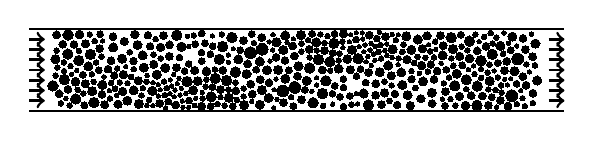
\begin{tikzpicture}[
scale=2.0,
]

\foreach \y in {0.65,1.3,1.95,2.6,3.25,3.9,4.55}
  \draw[color=black,line width=1.0pt,solid,->]
      (0mm,\y mm) -- (1mm, \y mm);
% inlet arrow

\foreach \y in {0.65,1.3,1.95,2.6,3.25,3.9,4.55}
  \draw[color=black,line width=1.0pt,solid,->]
      (33mm,\y mm) -- (34mm, \y mm);
% outlet arrow

% outer walls
\draw[line width=1pt] (0mm,0mm) -- (34mm,0mm);
\draw[line width=1pt] (0mm,5.2mm) -- (34mm,5.2mm);
\filldraw[line width=0pt] (31.902159mm,4.880683mm) circle (0.139755mm);
\filldraw[line width=0pt] (10.132162mm,4.093149mm) circle (0.138503mm);
\filldraw[line width=0pt] (30.969474mm,4.127407mm) circle (0.139086mm);
\filldraw[line width=0pt] (30.444063mm,4.291359mm) circle (0.138665mm);
\filldraw[line width=0pt] (30.148560mm,4.952732mm) circle (0.139398mm);
\filldraw[line width=0pt] (21.259932mm,3.757617mm) circle (0.138874mm);
\filldraw[line width=0pt] (4.676123mm,4.447397mm) circle (0.138741mm);
\filldraw[line width=0pt] (8.949880mm,1.101227mm) circle (0.137175mm);
\filldraw[line width=0pt] (22.592900mm,3.845908mm) circle (0.137855mm);
\filldraw[line width=0pt] (8.674888mm,0.201377mm) circle (0.139054mm);
\filldraw[line width=0pt] (14.143777mm,0.611821mm) circle (0.139339mm);
\filldraw[line width=0pt] (31.224078mm,1.289528mm) circle (0.138869mm);
\filldraw[line width=0pt] (15.487198mm,4.844206mm) circle (0.139782mm);
\filldraw[line width=0pt] (31.771043mm,2.480915mm) circle (0.139632mm);
\filldraw[line width=0pt] (9.407770mm,1.736749mm) circle (0.138835mm);
\filldraw[line width=0pt] (9.770237mm,0.236518mm) circle (0.138513mm);
\filldraw[line width=0pt] (15.291087mm,3.166535mm) circle (0.139854mm);
\filldraw[line width=0pt] (9.963742mm,1.109633mm) circle (0.139531mm);
\filldraw[line width=0pt] (20.792104mm,1.103777mm) circle (0.138848mm);
\filldraw[line width=0pt] (24.789923mm,2.381274mm) circle (0.139043mm);
\filldraw[line width=0pt] (22.249380mm,4.994797mm) circle (0.139155mm);
\filldraw[line width=0pt] (27.901102mm,2.626849mm) circle (0.139921mm);
\filldraw[line width=0pt] (16.384172mm,4.348901mm) circle (0.138589mm);
\filldraw[line width=0pt] (19.927414mm,4.014550mm) circle (0.139057mm);
\filldraw[line width=0pt] (6.133579mm,2.816454mm) circle (0.139181mm);
\filldraw[line width=0pt] (7.864709mm,0.334403mm) circle (0.139534mm);
\filldraw[line width=0pt] (15.746136mm,0.743515mm) circle (0.139109mm);
\filldraw[line width=0pt] (7.872138mm,1.797924mm) circle (0.138905mm);
\filldraw[line width=0pt] (15.540087mm,0.202128mm) circle (0.139979mm);
\filldraw[line width=0pt] (10.503964mm,0.348933mm) circle (0.139480mm);
\filldraw[line width=0pt] (9.665134mm,1.437424mm) circle (0.138971mm);
\filldraw[line width=0pt] (8.964672mm,1.975267mm) circle (0.138265mm);
\filldraw[line width=0pt] (10.063356mm,4.741980mm) circle (0.139579mm);
\filldraw[line width=0pt] (23.428188mm,2.945236mm) circle (0.139033mm);
\filldraw[line width=0pt] (21.650636mm,3.870711mm) circle (0.138217mm);
\filldraw[line width=0pt] (30.376882mm,1.649633mm) circle (0.138764mm);
\filldraw[line width=0pt] (9.729186mm,0.625280mm) circle (0.137022mm);
\filldraw[line width=0pt] (23.061298mm,4.861263mm) circle (0.138821mm);
\filldraw[line width=0pt] (20.863424mm,0.454159mm) circle (0.140199mm);
\filldraw[line width=0pt] (20.958077mm,4.087251mm) circle (0.137443mm);
\filldraw[line width=0pt] (9.055093mm,1.585056mm) circle (0.138885mm);
\filldraw[line width=0pt] (11.641671mm,4.764299mm) circle (0.139807mm);
\filldraw[line width=0pt] (22.717519mm,3.520873mm) circle (0.139085mm);
\filldraw[line width=0pt] (8.332031mm,1.349266mm) circle (0.138229mm);
\filldraw[line width=0pt] (18.267159mm,1.643874mm) circle (0.139483mm);
\filldraw[line width=0pt] (20.420929mm,4.845512mm) circle (0.138853mm);
\filldraw[line width=0pt] (19.282100mm,0.429216mm) circle (0.139476mm);
\filldraw[line width=0pt] (21.189264mm,4.569077mm) circle (0.137595mm);
\filldraw[line width=0pt] (28.225031mm,2.864593mm) circle (0.139409mm);
\filldraw[line width=0pt] (12.660696mm,3.086504mm) circle (0.139114mm);
\filldraw[line width=0pt] (3.027663mm,2.565862mm) circle (0.139737mm);
\filldraw[line width=0pt] (15.245500mm,4.387543mm) circle (0.139551mm);
\filldraw[line width=0pt] (21.868004mm,3.608024mm) circle (0.138429mm);
\filldraw[line width=0pt] (12.967269mm,3.946799mm) circle (0.139354mm);
\filldraw[line width=0pt] (30.201523mm,2.010995mm) circle (0.138334mm);
\filldraw[line width=0pt] (25.824675mm,3.900396mm) circle (0.139460mm);
\filldraw[line width=0pt] (9.274736mm,1.321411mm) circle (0.138983mm);
\filldraw[line width=0pt] (21.957960mm,3.218185mm) circle (0.138919mm);
\filldraw[line width=0pt] (21.975109mm,4.092289mm) circle (0.138324mm);
\filldraw[line width=0pt] (12.655784mm,3.551719mm) circle (0.137841mm);
\filldraw[line width=0pt] (10.995816mm,1.179620mm) circle (0.139468mm);
\filldraw[line width=0pt] (26.167414mm,3.030902mm) circle (0.139579mm);
\filldraw[line width=0pt] (23.054766mm,3.394457mm) circle (0.139667mm);
\filldraw[line width=0pt] (10.581130mm,0.800518mm) circle (0.139182mm);
\filldraw[line width=0pt] (21.341521mm,4.190331mm) circle (0.138807mm);
\filldraw[line width=0pt] (30.583859mm,2.050804mm) circle (0.138201mm);
\filldraw[line width=0pt] (26.247310mm,0.751561mm) circle (0.139028mm);
\filldraw[line width=0pt] (2.698244mm,2.327257mm) circle (0.138968mm);
\filldraw[line width=0pt] (29.688680mm,0.242872mm) circle (0.139191mm);
\filldraw[line width=0pt] (20.781365mm,4.968799mm) circle (0.137309mm);
\filldraw[line width=0pt] (16.782393mm,4.582307mm) circle (0.138570mm);
\filldraw[line width=0pt] (28.580833mm,4.403333mm) circle (0.138888mm);
\filldraw[line width=0pt] (21.515240mm,3.456316mm) circle (0.137601mm);
\filldraw[line width=0pt] (4.757410mm,2.168123mm) circle (0.140106mm);
\filldraw[line width=0pt] (9.214564mm,0.901229mm) circle (0.139110mm);
\filldraw[line width=0pt] (7.496260mm,2.251082mm) circle (0.139057mm);
\filldraw[line width=0pt] (18.261335mm,2.110241mm) circle (0.139110mm);
\filldraw[line width=0pt] (20.341497mm,4.393136mm) circle (0.138507mm);
\filldraw[line width=0pt] (7.481159mm,0.351066mm) circle (0.138118mm);
\filldraw[line width=0pt] (9.520040mm,2.074033mm) circle (0.139255mm);
\filldraw[line width=0pt] (23.439970mm,4.841358mm) circle (0.137661mm);
\filldraw[line width=0pt] (5.101877mm,1.294747mm) circle (0.139523mm);
\filldraw[line width=0pt] (21.735784mm,2.883067mm) circle (0.139225mm);
\filldraw[line width=0pt] (22.716201mm,4.253426mm) circle (0.138348mm);
\filldraw[line width=0pt] (29.534671mm,2.545359mm) circle (0.138982mm);
\filldraw[line width=0pt] (21.400171mm,3.123176mm) circle (0.138900mm);
\filldraw[line width=0pt] (15.559736mm,1.344829mm) circle (0.138163mm);
\filldraw[line width=0pt] (9.186667mm,2.311044mm) circle (0.139755mm);
\filldraw[line width=0pt] (9.585112mm,1.004652mm) circle (0.137857mm);
\filldraw[line width=0pt] (21.154137mm,4.960067mm) circle (0.138783mm);
\filldraw[line width=0pt] (15.681852mm,2.019302mm) circle (0.139392mm);
\filldraw[line width=0pt] (21.710525mm,4.296754mm) circle (0.139008mm);
\filldraw[line width=0pt] (15.470186mm,3.872658mm) circle (0.139940mm);
\filldraw[line width=0pt] (5.557064mm,0.984788mm) circle (0.138570mm);
\filldraw[line width=0pt] (2.340986mm,0.794282mm) circle (0.138672mm);
\filldraw[line width=0pt] (10.137902mm,0.228416mm) circle (0.138015mm);
\filldraw[line width=0pt] (17.956522mm,1.247480mm) circle (0.138220mm);
\filldraw[line width=0pt] (8.205326mm,0.943781mm) circle (0.139195mm);
\filldraw[line width=0pt] (8.206317mm,1.673469mm) circle (0.138562mm);
\filldraw[line width=0pt] (22.889491mm,0.637058mm) circle (0.175587mm);
\filldraw[line width=0pt] (23.018951mm,1.621364mm) circle (0.174911mm);
\filldraw[line width=0pt] (24.669577mm,3.432819mm) circle (0.174082mm);
\filldraw[line width=0pt] (4.254197mm,3.068418mm) circle (0.175321mm);
\filldraw[line width=0pt] (23.783605mm,4.209925mm) circle (0.175543mm);
\filldraw[line width=0pt] (29.316573mm,4.947144mm) circle (0.175421mm);
\filldraw[line width=0pt] (10.460252mm,4.801014mm) circle (0.175148mm);
\filldraw[line width=0pt] (26.667557mm,2.126338mm) circle (0.174294mm);
\filldraw[line width=0pt] (18.766931mm,4.317711mm) circle (0.173527mm);
\filldraw[line width=0pt] (22.307918mm,4.189890mm) circle (0.174642mm);
\filldraw[line width=0pt] (19.666447mm,3.210020mm) circle (0.174702mm);
\filldraw[line width=0pt] (20.465058mm,0.393284mm) circle (0.175076mm);
\filldraw[line width=0pt] (27.761746mm,1.379426mm) circle (0.176149mm);
\filldraw[line width=0pt] (13.631287mm,1.423917mm) circle (0.174417mm);
\filldraw[line width=0pt] (13.617280mm,0.921188mm) circle (0.173592mm);
\filldraw[line width=0pt] (3.989987mm,2.328826mm) circle (0.174538mm);
\filldraw[line width=0pt] (31.336718mm,0.809517mm) circle (0.174677mm);
\filldraw[line width=0pt] (2.221851mm,2.538811mm) circle (0.173186mm);
\filldraw[line width=0pt] (5.598661mm,2.704560mm) circle (0.175394mm);
\filldraw[line width=0pt] (28.712823mm,2.104499mm) circle (0.174247mm);
\filldraw[line width=0pt] (29.667097mm,4.660586mm) circle (0.175887mm);
\filldraw[line width=0pt] (12.158850mm,0.878742mm) circle (0.174327mm);
\filldraw[line width=0pt] (29.238444mm,2.945010mm) circle (0.175240mm);
\filldraw[line width=0pt] (6.254025mm,1.763206mm) circle (0.175109mm);
\filldraw[line width=0pt] (26.935087mm,2.869958mm) circle (0.176220mm);
\filldraw[line width=0pt] (14.280337mm,4.315607mm) circle (0.175268mm);
\filldraw[line width=0pt] (3.859922mm,4.856019mm) circle (0.174911mm);
\filldraw[line width=0pt] (4.167217mm,4.438767mm) circle (0.174911mm);
\filldraw[line width=0pt] (29.768694mm,2.135064mm) circle (0.174997mm);
\filldraw[line width=0pt] (12.246212mm,4.865084mm) circle (0.175500mm);
\filldraw[line width=0pt] (28.699509mm,2.654005mm) circle (0.173187mm);
\filldraw[line width=0pt] (29.442422mm,4.282195mm) circle (0.173920mm);
\filldraw[line width=0pt] (7.139541mm,0.985667mm) circle (0.174881mm);
\filldraw[line width=0pt] (30.978341mm,0.429468mm) circle (0.174816mm);
\filldraw[line width=0pt] (26.816909mm,3.344743mm) circle (0.175674mm);
\filldraw[line width=0pt] (28.288581mm,2.344131mm) circle (0.174908mm);
\filldraw[line width=0pt] (17.727532mm,4.490595mm) circle (0.174553mm);
\filldraw[line width=0pt] (28.338436mm,4.852768mm) circle (0.174017mm);
\filldraw[line width=0pt] (25.368926mm,4.210926mm) circle (0.139087mm);
\filldraw[line width=0pt] (29.124408mm,2.435447mm) circle (0.174604mm);
\filldraw[line width=0pt] (17.306441mm,4.269562mm) circle (0.174273mm);
\filldraw[line width=0pt] (17.294135mm,3.773496mm) circle (0.174779mm);
\filldraw[line width=0pt] (2.583863mm,0.342728mm) circle (0.175112mm);
\filldraw[line width=0pt] (31.482526mm,0.305858mm) circle (0.174744mm);
\filldraw[line width=0pt] (19.120074mm,2.561459mm) circle (0.173902mm);
\filldraw[line width=0pt] (17.814921mm,3.395546mm) circle (0.175662mm);
\filldraw[line width=0pt] (2.635886mm,2.849353mm) circle (0.175431mm);
\filldraw[line width=0pt] (5.761396mm,1.813773mm) circle (0.173855mm);
\filldraw[line width=0pt] (1.758605mm,3.823196mm) circle (0.175100mm);
\filldraw[line width=0pt] (18.956710mm,4.754144mm) circle (0.174849mm);
\filldraw[line width=0pt] (23.293093mm,4.492919mm) circle (0.175808mm);
\filldraw[line width=0pt] (25.163686mm,3.377039mm) circle (0.174465mm);
\filldraw[line width=0pt] (11.208832mm,1.550597mm) circle (0.173996mm);
\filldraw[line width=0pt] (1.799736mm,2.760888mm) circle (0.175265mm);
\filldraw[line width=0pt] (26.333912mm,1.757959mm) circle (0.175562mm);
\filldraw[line width=0pt] (2.022174mm,0.485836mm) circle (0.175011mm);
\filldraw[line width=0pt] (1.687421mm,2.249053mm) circle (0.175240mm);
\filldraw[line width=0pt] (30.100719mm,3.633031mm) circle (0.175650mm);
\filldraw[line width=0pt] (29.972827mm,1.628562mm) circle (0.174794mm);
\filldraw[line width=0pt] (3.157987mm,3.814339mm) circle (0.174742mm);
\filldraw[line width=0pt] (27.835200mm,3.851379mm) circle (0.175358mm);
\filldraw[line width=0pt] (22.351742mm,3.323650mm) circle (0.172390mm);
\filldraw[line width=0pt] (26.759592mm,0.758441mm) circle (0.174609mm);
\filldraw[line width=0pt] (23.699647mm,3.749544mm) circle (0.175656mm);
\filldraw[line width=0pt] (13.109305mm,1.800490mm) circle (0.176010mm);
\filldraw[line width=0pt] (28.899223mm,4.706869mm) circle (0.173675mm);
\filldraw[line width=0pt] (23.465632mm,3.341794mm) circle (0.174759mm);
\filldraw[line width=0pt] (13.197949mm,0.708236mm) circle (0.175170mm);
\filldraw[line width=0pt] (29.612820mm,1.331179mm) circle (0.175106mm);
\filldraw[line width=0pt] (25.713998mm,3.409409mm) circle (0.175029mm);
\filldraw[line width=0pt] (6.392401mm,3.729278mm) circle (0.182493mm);
\filldraw[line width=0pt] (5.210615mm,1.787221mm) circle (0.174404mm);
\filldraw[line width=0pt] (5.139389mm,0.796689mm) circle (0.175307mm);
\filldraw[line width=0pt] (24.530531mm,1.463376mm) circle (0.182103mm);
\filldraw[line width=0pt] (6.647252mm,2.660703mm) circle (0.174795mm);
\filldraw[line width=0pt] (7.905157mm,3.571419mm) circle (0.174554mm);
\filldraw[line width=0pt] (24.276618mm,2.533909mm) circle (0.174887mm);
\filldraw[line width=0pt] (18.275326mm,3.841862mm) circle (0.173331mm);
\filldraw[line width=0pt] (24.448319mm,3.042224mm) circle (0.183092mm);
\filldraw[line width=0pt] (31.993264mm,0.496317mm) circle (0.182068mm);
\filldraw[line width=0pt] (3.450614mm,1.110648mm) circle (0.175502mm);
\filldraw[line width=0pt] (31.584697mm,2.961299mm) circle (0.174944mm);
\filldraw[line width=0pt] (27.061443mm,0.340269mm) circle (0.176070mm);
\filldraw[line width=0pt] (22.182286mm,3.746330mm) circle (0.175533mm);
\filldraw[line width=0pt] (4.106395mm,1.850536mm) circle (0.175240mm);
\filldraw[line width=0pt] (32.123961mm,2.896973mm) circle (0.182033mm);
\filldraw[line width=0pt] (12.421098mm,0.333525mm) circle (0.174669mm);
\filldraw[line width=0pt] (18.501632mm,4.863275mm) circle (0.174116mm);
\filldraw[line width=0pt] (16.645866mm,0.879041mm) circle (0.176304mm);
\filldraw[line width=0pt] (5.458788mm,1.402116mm) circle (0.182840mm);
\filldraw[line width=0pt] (11.258305mm,1.989449mm) circle (0.174337mm);
\filldraw[line width=0pt] (6.477299mm,2.157066mm) circle (0.183358mm);
\filldraw[line width=0pt] (12.649395mm,1.353810mm) circle (0.175026mm);
\filldraw[line width=0pt] (8.613054mm,1.004890mm) circle (0.175778mm);
\filldraw[line width=0pt] (18.673852mm,0.327310mm) circle (0.176480mm);
\filldraw[line width=0pt] (30.009169mm,1.160477mm) circle (0.173969mm);
\filldraw[line width=0pt] (7.630014mm,0.701137mm) circle (0.175323mm);
\filldraw[line width=0pt] (29.161950mm,1.371632mm) circle (0.173996mm);
\filldraw[line width=0pt] (8.035363mm,4.561948mm) circle (0.176237mm);
\filldraw[line width=0pt] (25.466409mm,3.794563mm) circle (0.181481mm);
\filldraw[line width=0pt] (11.800508mm,2.635709mm) circle (0.174806mm);
\filldraw[line width=0pt] (11.964952mm,0.443212mm) circle (0.175853mm);
\filldraw[line width=0pt] (7.224775mm,1.447369mm) circle (0.176442mm);
\filldraw[line width=0pt] (25.784834mm,4.400780mm) circle (0.175985mm);
\filldraw[line width=0pt] (25.327849mm,2.495087mm) circle (0.175663mm);
\filldraw[line width=0pt] (7.458653mm,1.849351mm) circle (0.175047mm);
\filldraw[line width=0pt] (11.024815mm,0.791497mm) circle (0.173501mm);
\filldraw[line width=0pt] (27.473379mm,4.086252mm) circle (0.175169mm);
\filldraw[line width=0pt] (3.092924mm,1.344155mm) circle (0.176095mm);
\filldraw[line width=0pt] (19.896484mm,4.405340mm) circle (0.173691mm);
\filldraw[line width=0pt] (2.213668mm,3.089311mm) circle (0.174785mm);
\filldraw[line width=0pt] (22.560492mm,1.860729mm) circle (0.182268mm);
\filldraw[line width=0pt] (19.711003mm,3.644348mm) circle (0.174131mm);
\filldraw[line width=0pt] (19.961547mm,2.031603mm) circle (0.214231mm);
\filldraw[line width=0pt] (8.362102mm,3.337220mm) circle (0.183979mm);
\filldraw[line width=0pt] (8.738781mm,1.447642mm) circle (0.175741mm);
\filldraw[line width=0pt] (8.570044mm,1.870747mm) circle (0.173582mm);
\filldraw[line width=0pt] (21.048364mm,2.655497mm) circle (0.215597mm);
\filldraw[line width=0pt] (11.651572mm,1.515461mm) circle (0.217859mm);
\filldraw[line width=0pt] (19.973444mm,1.488821mm) circle (0.214819mm);
\filldraw[line width=0pt] (4.589712mm,3.442332mm) circle (0.176714mm);
\filldraw[line width=0pt] (19.398615mm,4.898068mm) circle (0.218095mm);
\filldraw[line width=0pt] (11.170973mm,4.297055mm) circle (0.213169mm);
\filldraw[line width=0pt] (26.497872mm,2.616318mm) circle (0.214002mm);
\filldraw[line width=0pt] (27.414554mm,4.840253mm) circle (0.216563mm);
\filldraw[line width=0pt] (30.581854mm,3.857443mm) circle (0.217006mm);
\filldraw[line width=0pt] (27.508392mm,2.893516mm) circle (0.217371mm);
\filldraw[line width=0pt] (20.371213mm,0.952242mm) circle (0.214771mm);
\filldraw[line width=0pt] (12.942633mm,0.297053mm) circle (0.216938mm);
\filldraw[line width=0pt] (14.425632mm,2.622341mm) circle (0.218642mm);
\filldraw[line width=0pt] (16.497239mm,2.574849mm) circle (0.218593mm);
\filldraw[line width=0pt] (10.961885mm,4.923457mm) circle (0.216125mm);
\filldraw[line width=0pt] (19.264803mm,1.091921mm) circle (0.214337mm);
\filldraw[line width=0pt] (10.158045mm,0.662207mm) circle (0.214146mm);
\filldraw[line width=0pt] (10.951115mm,3.707225mm) circle (0.214433mm);
\filldraw[line width=0pt] (11.515919mm,3.598018mm) circle (0.213838mm);
\filldraw[line width=0pt] (4.512105mm,4.868637mm) circle (0.215597mm);
\filldraw[line width=0pt] (3.511021mm,0.353735mm) circle (0.217768mm);
\filldraw[line width=0pt] (10.552164mm,4.242337mm) circle (0.214840mm);
\filldraw[line width=0pt] (29.758107mm,3.050058mm) circle (0.217485mm);
\filldraw[line width=0pt] (3.416355mm,2.300814mm) circle (0.217462mm);
\filldraw[line width=0pt] (17.515155mm,1.342599mm) circle (0.217972mm);
\filldraw[line width=0pt] (19.405118mm,1.598251mm) circle (0.213835mm);
\filldraw[line width=0pt] (30.955471mm,1.724310mm) circle (0.217981mm);
\filldraw[line width=0pt] (10.962214mm,3.163724mm) circle (0.215381mm);
\filldraw[line width=0pt] (19.751576mm,0.898198mm) circle (0.212912mm);
\filldraw[line width=0pt] (10.133518mm,2.991283mm) circle (0.212927mm);
\filldraw[line width=0pt] (20.791613mm,2.205220mm) circle (0.213204mm);
\filldraw[line width=0pt] (9.877854mm,2.542461mm) circle (0.213577mm);
\filldraw[line width=0pt] (26.412947mm,0.329289mm) circle (0.214186mm);
\filldraw[line width=0pt] (21.373565mm,1.798386mm) circle (0.214017mm);
\filldraw[line width=0pt] (11.657232mm,4.105820mm) circle (0.212476mm);
\filldraw[line width=0pt] (4.425596mm,2.581928mm) circle (0.213470mm);
\filldraw[line width=0pt] (29.386590mm,0.878674mm) circle (0.217522mm);
\filldraw[line width=0pt] (9.548803mm,3.395039mm) circle (0.214759mm);
\filldraw[line width=0pt] (19.962446mm,0.272399mm) circle (0.214251mm);
\filldraw[line width=0pt] (8.842779mm,0.594422mm) circle (0.215726mm);
\filldraw[line width=0pt] (22.080896mm,4.599083mm) circle (0.216104mm);
\filldraw[line width=0pt] (11.528839mm,0.299972mm) circle (0.218532mm);
\filldraw[line width=0pt] (13.407378mm,3.852066mm) circle (0.216709mm);
\filldraw[line width=0pt] (31.979358mm,3.442380mm) circle (0.246966mm);
\filldraw[line width=0pt] (16.787215mm,0.310727mm) circle (0.219276mm);
\filldraw[line width=0pt] (20.766088mm,4.534097mm) circle (0.213321mm);
\filldraw[line width=0pt] (29.926432mm,0.675381mm) circle (0.246902mm);
\filldraw[line width=0pt] (30.413971mm,0.316716mm) circle (0.246811mm);
\filldraw[line width=0pt] (17.982835mm,4.898130mm) circle (0.216144mm);
\filldraw[line width=0pt] (5.330605mm,4.721111mm) circle (0.246989mm);
\filldraw[line width=0pt] (14.138609mm,4.881951mm) circle (0.217231mm);
\filldraw[line width=0pt] (26.119223mm,4.794916mm) circle (0.246684mm);
\filldraw[line width=0pt] (28.782958mm,0.954496mm) circle (0.246457mm);
\filldraw[line width=0pt] (2.850270mm,4.220288mm) circle (0.247355mm);
\filldraw[line width=0pt] (31.356957mm,2.184128mm) circle (0.246757mm);
\filldraw[line width=0pt] (1.755281mm,4.833714mm) circle (0.246717mm);
\filldraw[line width=0pt] (13.880037mm,2.988786mm) circle (0.246768mm);
\filldraw[line width=0pt] (14.678531mm,1.990034mm) circle (0.247083mm);
\filldraw[line width=0pt] (23.378238mm,0.385170mm) circle (0.234931mm);
\filldraw[line width=0pt] (5.014255mm,2.658447mm) circle (0.246110mm);
\filldraw[line width=0pt] (24.292345mm,2.024951mm) circle (0.234784mm);
\filldraw[line width=0pt] (23.232451mm,1.085502mm) circle (0.234988mm);
\filldraw[line width=0pt] (15.238218mm,1.790124mm) circle (0.247384mm);
\filldraw[line width=0pt] (25.510362mm,2.945147mm) circle (0.234910mm);
\filldraw[line width=0pt] (19.274463mm,3.681464mm) circle (0.217412mm);
\filldraw[line width=0pt] (22.388903mm,0.401819mm) circle (0.246625mm);
\filldraw[line width=0pt] (17.799368mm,3.916697mm) circle (0.247408mm);
\filldraw[line width=0pt] (28.454802mm,3.820798mm) circle (0.246563mm);
\filldraw[line width=0pt] (16.747954mm,4.127669mm) circle (0.246810mm);
\filldraw[line width=0pt] (7.544650mm,4.810411mm) circle (0.234781mm);
\filldraw[line width=0pt] (26.438053mm,1.229725mm) circle (0.247019mm);
\filldraw[line width=0pt] (31.363568mm,4.602637mm) circle (0.246832mm);
\filldraw[line width=0pt] (30.333856mm,3.149317mm) circle (0.247936mm);
\filldraw[line width=0pt] (25.594005mm,0.473317mm) circle (0.247330mm);
\filldraw[line width=0pt] (8.922352mm,4.196783mm) circle (0.247330mm);
\filldraw[line width=0pt] (14.778004mm,4.667525mm) circle (0.247045mm);
\filldraw[line width=0pt] (4.485629mm,3.964793mm) circle (0.247400mm);
\filldraw[line width=0pt] (16.245979mm,3.205085mm) circle (0.246870mm);
\filldraw[line width=0pt] (25.910213mm,2.535864mm) circle (0.247051mm);
\filldraw[line width=0pt] (6.042267mm,4.416632mm) circle (0.259461mm);
\filldraw[line width=0pt] (9.316687mm,0.380225mm) circle (0.246524mm);
\filldraw[line width=0pt] (5.208660mm,3.188712mm) circle (0.248072mm);
\filldraw[line width=0pt] (18.620745mm,2.606416mm) circle (0.246998mm);
\filldraw[line width=0pt] (5.412980mm,2.248860mm) circle (0.233972mm);
\filldraw[line width=0pt] (29.167968mm,0.359570mm) circle (0.247211mm);
\filldraw[line width=0pt] (21.603878mm,4.811253mm) circle (0.247636mm);
\filldraw[line width=0pt] (8.535077mm,4.794019mm) circle (0.247332mm);
\filldraw[line width=0pt] (8.906492mm,3.467749mm) circle (0.247034mm);
\filldraw[line width=0pt] (16.849883mm,3.496118mm) circle (0.246448mm);
\filldraw[line width=0pt] (31.996306mm,1.129844mm) circle (0.247125mm);
\filldraw[line width=0pt] (25.716075mm,2.004908mm) circle (0.247123mm);
\filldraw[line width=0pt] (4.628403mm,1.054834mm) circle (0.246401mm);
\filldraw[line width=0pt] (3.587249mm,4.261905mm) circle (0.259221mm);
\filldraw[line width=0pt] (28.073239mm,0.977061mm) circle (0.246873mm);
\filldraw[line width=0pt] (17.046463mm,2.209544mm) circle (0.246873mm);
\filldraw[line width=0pt] (7.688161mm,4.109231mm) circle (0.235072mm);
\filldraw[line width=0pt] (24.883945mm,0.778378mm) circle (0.259786mm);
\filldraw[line width=0pt] (22.632004mm,4.714140mm) circle (0.246891mm);
\filldraw[line width=0pt] (27.334294mm,0.933972mm) circle (0.259797mm);
\filldraw[line width=0pt] (30.185274mm,2.562040mm) circle (0.247791mm);
\filldraw[line width=0pt] (18.765930mm,3.828768mm) circle (0.247546mm);
\filldraw[line width=0pt] (6.626389mm,3.169561mm) circle (0.235431mm);
\filldraw[line width=0pt] (8.295639mm,0.481049mm) circle (0.247632mm);
\filldraw[line width=0pt] (2.468101mm,1.377149mm) circle (0.246803mm);
\filldraw[line width=0pt] (13.124906mm,1.281216mm) circle (0.246543mm);
\filldraw[line width=0pt] (7.924591mm,2.961275mm) circle (0.259222mm);
\filldraw[line width=0pt] (22.004487mm,1.000612mm) circle (0.247709mm);
\filldraw[line width=0pt] (31.510330mm,3.902079mm) circle (0.247443mm);
\filldraw[line width=0pt] (9.357122mm,2.747806mm) circle (0.247348mm);
\filldraw[line width=0pt] (2.142291mm,4.238869mm) circle (0.246433mm);
\filldraw[line width=0pt] (1.911025mm,1.089591mm) circle (0.247449mm);
\filldraw[line width=0pt] (15.685116mm,3.406057mm) circle (0.247617mm);
\filldraw[line width=0pt] (14.174729mm,1.067502mm) circle (0.246460mm);
\filldraw[line width=0pt] (6.716867mm,4.856612mm) circle (0.266196mm);
\filldraw[line width=0pt] (12.158461mm,1.366622mm) circle (0.246830mm);
\filldraw[line width=0pt] (19.966646mm,4.897554mm) circle (0.260389mm);
\filldraw[line width=0pt] (29.014059mm,4.106865mm) circle (0.247027mm);
\filldraw[line width=0pt] (14.073728mm,1.703404mm) circle (0.248930mm);
\filldraw[line width=0pt] (6.927002mm,1.921610mm) circle (0.260327mm);
\filldraw[line width=0pt] (13.617877mm,4.483907mm) circle (0.246717mm);
\filldraw[line width=0pt] (23.000560mm,2.234343mm) circle (0.260333mm);
\filldraw[line width=0pt] (25.270989mm,4.768221mm) circle (0.260414mm);
\filldraw[line width=0pt] (24.207682mm,0.338252mm) circle (0.266188mm);
\filldraw[line width=0pt] (5.652679mm,0.427657mm) circle (0.259552mm);
\filldraw[line width=0pt] (12.302011mm,2.586686mm) circle (0.247073mm);
\filldraw[line width=0pt] (27.352330mm,3.467596mm) circle (0.260438mm);
\filldraw[line width=0pt] (5.951667mm,1.238074mm) circle (0.266840mm);
\filldraw[line width=0pt] (3.570883mm,1.728318mm) circle (0.260248mm);
\filldraw[line width=0pt] (20.403439mm,2.619050mm) circle (0.260660mm);
\filldraw[line width=0pt] (31.555874mm,1.637019mm) circle (0.247329mm);
\filldraw[line width=0pt] (24.976013mm,3.956404mm) circle (0.266681mm);
\filldraw[line width=0pt] (10.956286mm,0.296757mm) circle (0.260332mm);
\filldraw[line width=0pt] (22.571286mm,1.149903mm) circle (0.266181mm);
\filldraw[line width=0pt] (23.999240mm,3.274000mm) circle (0.260128mm);
\filldraw[line width=0pt] (8.352453mm,4.046981mm) circle (0.265668mm);
\filldraw[line width=0pt] (21.564880mm,2.447521mm) circle (0.249152mm);
\filldraw[line width=0pt] (24.037528mm,1.007271mm) circle (0.285796mm);
\filldraw[line width=0pt] (14.650236mm,3.141452mm) circle (0.289018mm);
\filldraw[line width=0pt] (17.303424mm,0.711623mm) circle (0.247856mm);
\filldraw[line width=0pt] (4.804021mm,0.401093mm) circle (0.248961mm);
\filldraw[line width=0pt] (26.297828mm,4.143328mm) circle (0.248654mm);
\filldraw[line width=0pt] (10.519229mm,2.574028mm) circle (0.260364mm);
\filldraw[line width=0pt] (10.718068mm,1.900168mm) circle (0.278923mm);
\filldraw[line width=0pt] (22.018465mm,1.730159mm) circle (0.247170mm);
\filldraw[line width=0pt] (2.948445mm,1.860154mm) circle (0.279278mm);
\filldraw[line width=0pt] (24.927755mm,2.885253mm) circle (0.265980mm);
\filldraw[line width=0pt] (16.148622mm,0.528168mm) circle (0.247149mm);
\filldraw[line width=0pt] (30.694065mm,4.719179mm) circle (0.287640mm);
\filldraw[line width=0pt] (5.992685mm,2.308650mm) circle (0.266257mm);
\filldraw[line width=0pt] (6.886977mm,4.190822mm) circle (0.285872mm);
\filldraw[line width=0pt] (15.815287mm,2.610195mm) circle (0.287863mm);
\filldraw[line width=0pt] (15.109778mm,2.585805mm) circle (0.287703mm);
\filldraw[line width=0pt] (6.644128mm,1.313357mm) circle (0.285879mm);
\filldraw[line width=0pt] (11.262098mm,2.512880mm) circle (0.279099mm);
\filldraw[line width=0pt] (30.823246mm,2.528012mm) circle (0.288220mm);
\filldraw[line width=0pt] (17.634108mm,1.914813mm) circle (0.287666mm);
\filldraw[line width=0pt] (7.215603mm,3.535801mm) circle (0.285337mm);
\filldraw[line width=0pt] (32.264181mm,1.936298mm) circle (0.288835mm);
\filldraw[line width=0pt] (16.277951mm,2.051619mm) circle (0.288059mm);
\filldraw[line width=0pt] (20.207204mm,3.297794mm) circle (0.279684mm);
\filldraw[line width=0pt] (16.144202mm,3.870733mm) circle (0.288787mm);
\filldraw[line width=0pt] (13.812802mm,2.346938mm) circle (0.287863mm);
\filldraw[line width=0pt] (5.346621mm,4.035213mm) circle (0.289110mm);
\filldraw[line width=0pt] (21.244020mm,1.113139mm) circle (0.291096mm);
\filldraw[line width=0pt] (15.212352mm,0.829550mm) circle (0.287856mm);
\filldraw[line width=0pt] (29.930266mm,4.132884mm) circle (0.289975mm);
\filldraw[line width=0pt] (25.018296mm,1.876399mm) circle (0.288720mm);
\filldraw[line width=0pt] (8.651224mm,2.735777mm) circle (0.288496mm);
\filldraw[line width=0pt] (23.637639mm,2.443873mm) circle (0.285130mm);
\filldraw[line width=0pt] (14.783037mm,1.325871mm) circle (0.288183mm);
\filldraw[line width=0pt] (17.109957mm,2.847011mm) circle (0.287945mm);
\filldraw[line width=0pt] (6.970174mm,0.450130mm) circle (0.290425mm);
\filldraw[line width=0pt] (27.720608mm,0.345050mm) circle (0.279325mm);
\filldraw[line width=0pt] (14.656618mm,0.397870mm) circle (0.285269mm);
\filldraw[line width=0pt] (20.509286mm,3.883179mm) circle (0.290195mm);
\filldraw[line width=0pt] (5.908782mm,3.319853mm) circle (0.288671mm);
\filldraw[line width=0pt] (4.009092mm,1.255762mm) circle (0.290035mm);
\filldraw[line width=0pt] (19.659370mm,2.682576mm) circle (0.280405mm);
\filldraw[line width=0pt] (7.287332mm,2.755798mm) circle (0.286333mm);
\filldraw[line width=0pt] (26.913452mm,3.939239mm) circle (0.289258mm);
\filldraw[line width=0pt] (23.952617mm,4.747323mm) circle (0.289828mm);
\filldraw[line width=0pt] (23.092122mm,3.922701mm) circle (0.290399mm);
\filldraw[line width=0pt] (13.291079mm,3.279358mm) circle (0.289388mm);
\filldraw[line width=0pt] (7.831719mm,1.275177mm) circle (0.294774mm);
\filldraw[line width=0pt] (25.578431mm,1.158469mm) circle (0.290137mm);
\filldraw[line width=0pt] (24.279369mm,3.886159mm) circle (0.285807mm);
\filldraw[line width=0pt] (23.707936mm,1.656794mm) circle (0.285075mm);
\filldraw[line width=0pt] (32.156106mm,4.279946mm) circle (0.288596mm);
\filldraw[line width=0pt] (4.658632mm,1.659609mm) circle (0.289217mm);
\filldraw[line width=0pt] (27.974273mm,3.333543mm) circle (0.279208mm);
\filldraw[line width=0pt] (15.709568mm,4.361499mm) circle (0.293098mm);
\filldraw[line width=0pt] (8.115328mm,2.308957mm) circle (0.289376mm);
\filldraw[line width=0pt] (27.153079mm,2.366007mm) circle (0.289835mm);
\filldraw[line width=0pt] (6.244382mm,0.655568mm) circle (0.288198mm);
\filldraw[line width=0pt] (9.680667mm,4.084281mm) circle (0.292300mm);
\filldraw[line width=0pt] (22.269102mm,2.463210mm) circle (0.288990mm);
\filldraw[line width=0pt] (3.204252mm,4.850607mm) circle (0.279762mm);
\filldraw[line width=0pt] (22.808094mm,2.884079mm) circle (0.288912mm);
\filldraw[line width=0pt] (13.660080mm,0.378388mm) circle (0.290706mm);
\filldraw[line width=0pt] (10.415059mm,1.310876mm) circle (0.289033mm);
\filldraw[line width=0pt] (1.672317mm,3.292116mm) circle (0.290106mm);
\filldraw[line width=0pt] (24.681244mm,4.539631mm) circle (0.289049mm);
\filldraw[line width=0pt] (17.266569mm,4.814822mm) circle (0.290240mm);
\filldraw[line width=0pt] (26.264748mm,3.528486mm) circle (0.288998mm);
\filldraw[line width=0pt] (29.249521mm,1.901027mm) circle (0.290225mm);
\filldraw[line width=0pt] (3.767654mm,2.832642mm) circle (0.289974mm);
\filldraw[line width=0pt] (18.235734mm,4.358213mm) circle (0.291912mm);
\filldraw[line width=0pt] (3.158452mm,3.209124mm) circle (0.325521mm);
\filldraw[line width=0pt] (16.265575mm,4.795510mm) circle (0.287472mm);
\filldraw[line width=0pt] (12.690258mm,0.838873mm) circle (0.290913mm);
\filldraw[line width=0pt] (2.962542mm,0.761694mm) circle (0.327425mm);
\filldraw[line width=0pt] (21.546072mm,0.383547mm) circle (0.330533mm);
\filldraw[line width=0pt] (20.894580mm,3.323272mm) circle (0.332241mm);
\filldraw[line width=0pt] (2.461316mm,3.617426mm) circle (0.326281mm);
\filldraw[line width=0pt] (28.441650mm,0.361602mm) circle (0.330588mm);
\filldraw[line width=0pt] (27.031346mm,1.600566mm) circle (0.331571mm);
\filldraw[line width=0pt] (11.823175mm,2.072724mm) circle (0.326882mm);
\filldraw[line width=0pt] (13.100491mm,2.465139mm) circle (0.331293mm);
\filldraw[line width=0pt] (28.461687mm,1.577583mm) circle (0.325415mm);
\filldraw[line width=0pt] (3.894523mm,3.595722mm) circle (0.331263mm);
\filldraw[line width=0pt] (27.965447mm,4.434735mm) circle (0.327513mm);
\filldraw[line width=0pt] (12.079982mm,3.279811mm) circle (0.330977mm);
\filldraw[line width=0pt] (10.030765mm,1.870511mm) circle (0.332313mm);
\filldraw[line width=0pt] (11.565929mm,0.900394mm) circle (0.325158mm);
\filldraw[line width=0pt] (12.545474mm,1.935869mm) circle (0.332436mm);
\filldraw[line width=0pt] (19.104899mm,3.128058mm) circle (0.327429mm);
\filldraw[line width=0pt] (2.479701mm,4.830947mm) circle (0.331956mm);
\filldraw[line width=0pt] (18.037258mm,0.522011mm) circle (0.331472mm);
\filldraw[line width=0pt] (29.412730mm,3.600798mm) circle (0.331074mm);
\filldraw[line width=0pt] (4.117483mm,0.536062mm) circle (0.331269mm);
\filldraw[line width=0pt] (26.806863mm,4.660372mm) circle (0.331423mm);
\filldraw[line width=0pt] (17.818928mm,2.727494mm) circle (0.331153mm);
\filldraw[line width=0pt] (12.291910mm,4.089987mm) circle (0.331529mm);
\filldraw[line width=0pt] (27.766425mm,1.987276mm) circle (0.325038mm);
\filldraw[line width=0pt] (18.631137mm,1.106164mm) circle (0.331228mm);
\filldraw[line width=0pt] (2.235046mm,1.997505mm) circle (0.333560mm);
\filldraw[line width=0pt] (9.376923mm,4.810977mm) circle (0.331069mm);
\filldraw[line width=0pt] (1.511951mm,1.596302mm) circle (0.330901mm);
\filldraw[line width=0pt] (12.883138mm,4.671071mm) circle (0.331254mm);
\filldraw[line width=0pt] (18.843142mm,1.916167mm) circle (0.331180mm);
\filldraw[line width=0pt] (28.692751mm,3.194530mm) circle (0.333741mm);
\filldraw[line width=0pt] (18.379338mm,3.259475mm) circle (0.332865mm);
\filldraw[line width=0pt] (19.360491mm,4.296554mm) circle (0.325356mm);
\filldraw[line width=0pt] (14.058245mm,3.700290mm) circle (0.372957mm);
\filldraw[line width=0pt] (16.868633mm,1.493581mm) circle (0.372898mm);
\filldraw[line width=0pt] (16.113202mm,1.273165mm) circle (0.373588mm);
\filldraw[line width=0pt] (30.648525mm,0.970660mm) circle (0.373598mm);
\filldraw[line width=0pt] (14.807191mm,3.920906mm) circle (0.373858mm);
\filldraw[line width=0pt] (31.026645mm,3.304579mm) circle (0.373711mm);

\end{tikzpicture}

  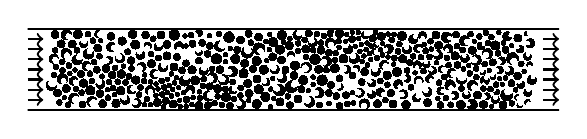
\begin{tikzpicture}[
scale=0.8,
%spy using outlines={rectangle,lens={scale=4}, size=0.4in, connect spies}
]

\begin{axis}[
  scale only axis,
  axis equal image,
  xmin = 0,
  xmax = 34,
  ymin = -0.2,
  ymax = 5.4,
  hide axis,
  ]

\addplot [color=black,solid,line width=1] table{
-1 0
35 0
};
\addplot [color=black,solid,line width=1] table{
-1 5.2 
35 5.2
};
% outer walls

\foreach \y in {0.65,1.3,1.95,2.6,3.25,3.9,4.55}
  \addplot[color=black,line width = 1.0pt,solid,->]
      plot coordinates{(0,\y)(1,\y)};
% inlet arrow

\foreach \y in {0.65,1.3,1.95,2.6,3.25,3.9,4.55}
  \addplot[color=black,line width = 1.0pt,solid,->]
      plot coordinates{(33,\y)(34,\y)};
% outlet arrow

\addplot [color=black,solid,fill=black,line width=0] table{ 
1.0271e+01 4.0931e+00
1.0268e+01 4.1202e+00
1.0260e+01 4.1462e+00
1.0247e+01 4.1701e+00
1.0230e+01 4.1911e+00
1.0209e+01 4.2083e+00
1.0185e+01 4.2211e+00
1.0159e+01 4.2290e+00
1.0132e+01 4.2317e+00
1.0105e+01 4.2290e+00
1.0079e+01 4.2211e+00
1.0055e+01 4.2083e+00
1.0034e+01 4.1911e+00
1.0017e+01 4.1701e+00
1.0004e+01 4.1462e+00
9.9963e+00 4.1202e+00
9.9937e+00 4.0931e+00
9.9963e+00 4.0661e+00
1.0004e+01 4.0401e+00
1.0017e+01 4.0162e+00
1.0034e+01 3.9952e+00
1.0055e+01 3.9780e+00
1.0079e+01 3.9652e+00
1.0105e+01 3.9573e+00
1.0132e+01 3.9546e+00
1.0159e+01 3.9573e+00
1.0185e+01 3.9652e+00
1.0209e+01 3.9780e+00
1.0230e+01 3.9952e+00
1.0247e+01 4.0162e+00
1.0260e+01 4.0401e+00
1.0268e+01 4.0661e+00
}; 
\addplot [color=black,solid,fill=black,line width=0] table{ 
3.1109e+01 4.1274e+00
3.1106e+01 4.1545e+00
3.1098e+01 4.1806e+00
3.1085e+01 4.2047e+00
3.1068e+01 4.2258e+00
3.1047e+01 4.2431e+00
3.1023e+01 4.2559e+00
3.0997e+01 4.2638e+00
3.0969e+01 4.2665e+00
3.0942e+01 4.2638e+00
3.0916e+01 4.2559e+00
3.0892e+01 4.2431e+00
3.0871e+01 4.2258e+00
3.0854e+01 4.2047e+00
3.0841e+01 4.1806e+00
3.0833e+01 4.1545e+00
3.0830e+01 4.1274e+00
3.0833e+01 4.1003e+00
3.0841e+01 4.0742e+00
3.0854e+01 4.0501e+00
3.0871e+01 4.0291e+00
3.0892e+01 4.0118e+00
3.0916e+01 3.9989e+00
3.0942e+01 3.9910e+00
3.0969e+01 3.9883e+00
3.0997e+01 3.9910e+00
3.1023e+01 3.9989e+00
3.1047e+01 4.0118e+00
3.1068e+01 4.0291e+00
3.1085e+01 4.0501e+00
3.1098e+01 4.0742e+00
3.1106e+01 4.1003e+00
}; 
\addplot [color=black,solid,fill=black,line width=0] table{ 
3.0583e+01 4.2914e+00
3.0580e+01 4.3184e+00
3.0572e+01 4.3444e+00
3.0559e+01 4.3684e+00
3.0542e+01 4.3894e+00
3.0521e+01 4.4067e+00
3.0497e+01 4.4195e+00
3.0471e+01 4.4274e+00
3.0444e+01 4.4300e+00
3.0417e+01 4.4274e+00
3.0391e+01 4.4195e+00
3.0367e+01 4.4067e+00
3.0346e+01 4.3894e+00
3.0329e+01 4.3684e+00
3.0316e+01 4.3444e+00
3.0308e+01 4.3184e+00
3.0305e+01 4.2914e+00
3.0308e+01 4.2643e+00
3.0316e+01 4.2383e+00
3.0329e+01 4.2143e+00
3.0346e+01 4.1933e+00
3.0367e+01 4.1761e+00
3.0391e+01 4.1632e+00
3.0417e+01 4.1554e+00
3.0444e+01 4.1527e+00
3.0471e+01 4.1554e+00
3.0497e+01 4.1632e+00
3.0521e+01 4.1761e+00
3.0542e+01 4.1933e+00
3.0559e+01 4.2143e+00
3.0572e+01 4.2383e+00
3.0580e+01 4.2643e+00
}; 
\addplot [color=black,solid,fill=black,line width=0] table{ 
3.0288e+01 4.9527e+00
3.0285e+01 4.9799e+00
3.0277e+01 5.0061e+00
3.0264e+01 5.0302e+00
3.0247e+01 5.0513e+00
3.0226e+01 5.0686e+00
3.0202e+01 5.0815e+00
3.0176e+01 5.0895e+00
3.0149e+01 5.0921e+00
3.0121e+01 5.0895e+00
3.0095e+01 5.0815e+00
3.0071e+01 5.0686e+00
3.0050e+01 5.0513e+00
3.0033e+01 5.0302e+00
3.0020e+01 5.0061e+00
3.0012e+01 4.9799e+00
3.0009e+01 4.9527e+00
3.0012e+01 4.9255e+00
3.0020e+01 4.8994e+00
3.0033e+01 4.8753e+00
3.0050e+01 4.8542e+00
3.0071e+01 4.8368e+00
3.0095e+01 4.8239e+00
3.0121e+01 4.8160e+00
3.0149e+01 4.8133e+00
3.0176e+01 4.8160e+00
3.0202e+01 4.8239e+00
3.0226e+01 4.8368e+00
3.0247e+01 4.8542e+00
3.0264e+01 4.8753e+00
3.0277e+01 4.8994e+00
3.0285e+01 4.9255e+00
}; 
\addplot [color=black,solid,fill=black,line width=0] table{ 
2.1399e+01 3.7576e+00
2.1396e+01 3.7847e+00
2.1388e+01 3.8108e+00
2.1375e+01 3.8348e+00
2.1358e+01 3.8558e+00
2.1337e+01 3.8731e+00
2.1313e+01 3.8859e+00
2.1287e+01 3.8938e+00
2.1260e+01 3.8965e+00
2.1233e+01 3.8938e+00
2.1207e+01 3.8859e+00
2.1183e+01 3.8731e+00
2.1162e+01 3.8558e+00
2.1144e+01 3.8348e+00
2.1132e+01 3.8108e+00
2.1124e+01 3.7847e+00
2.1121e+01 3.7576e+00
2.1124e+01 3.7305e+00
2.1132e+01 3.7045e+00
2.1144e+01 3.6805e+00
2.1162e+01 3.6594e+00
2.1183e+01 3.6421e+00
2.1207e+01 3.6293e+00
2.1233e+01 3.6214e+00
2.1260e+01 3.6187e+00
2.1287e+01 3.6214e+00
2.1313e+01 3.6293e+00
2.1337e+01 3.6421e+00
2.1358e+01 3.6594e+00
2.1375e+01 3.6805e+00
2.1388e+01 3.7045e+00
2.1396e+01 3.7305e+00
}; 
\addplot [color=black,solid,fill=black,line width=0] table{ 
4.8149e+00 4.4474e+00
4.8122e+00 4.4745e+00
4.8043e+00 4.5005e+00
4.7915e+00 4.5245e+00
4.7742e+00 4.5455e+00
4.7532e+00 4.5628e+00
4.7292e+00 4.5756e+00
4.7032e+00 4.5835e+00
4.6761e+00 4.5861e+00
4.6491e+00 4.5835e+00
4.6230e+00 4.5756e+00
4.5990e+00 4.5628e+00
4.5780e+00 4.5455e+00
4.5608e+00 4.5245e+00
4.5479e+00 4.5005e+00
4.5400e+00 4.4745e+00
4.5374e+00 4.4474e+00
4.5400e+00 4.4203e+00
4.5479e+00 4.3943e+00
4.5608e+00 4.3703e+00
4.5780e+00 4.3493e+00
4.5990e+00 4.3320e+00
4.6230e+00 4.3192e+00
4.6491e+00 4.3113e+00
4.6761e+00 4.3087e+00
4.7032e+00 4.3113e+00
4.7292e+00 4.3192e+00
4.7532e+00 4.3320e+00
4.7742e+00 4.3493e+00
4.7915e+00 4.3703e+00
4.8043e+00 4.3943e+00
4.8122e+00 4.4203e+00
}; 
\addplot [color=black,solid,fill=black,line width=0] table{ 
9.0871e+00 1.1012e+00
9.0844e+00 1.1280e+00
9.0766e+00 1.1537e+00
9.0639e+00 1.1774e+00
9.0469e+00 1.1982e+00
9.0261e+00 1.2153e+00
9.0024e+00 1.2280e+00
8.9766e+00 1.2358e+00
8.9499e+00 1.2384e+00
8.9231e+00 1.2358e+00
8.8974e+00 1.2280e+00
8.8737e+00 1.2153e+00
8.8529e+00 1.1982e+00
8.8358e+00 1.1774e+00
8.8231e+00 1.1537e+00
8.8153e+00 1.1280e+00
8.8127e+00 1.1012e+00
8.8153e+00 1.0745e+00
8.8231e+00 1.0487e+00
8.8358e+00 1.0250e+00
8.8529e+00 1.0042e+00
8.8737e+00 9.8717e-01
8.8974e+00 9.7449e-01
8.9231e+00 9.6669e-01
8.9499e+00 9.6405e-01
8.9766e+00 9.6669e-01
9.0024e+00 9.7449e-01
9.0261e+00 9.8717e-01
9.0469e+00 1.0042e+00
9.0639e+00 1.0250e+00
9.0766e+00 1.0487e+00
9.0844e+00 1.0745e+00
}; 
\addplot [color=black,solid,fill=black,line width=0] table{ 
2.2731e+01 3.8459e+00
2.2728e+01 3.8728e+00
2.2720e+01 3.8987e+00
2.2708e+01 3.9225e+00
2.2690e+01 3.9434e+00
2.2669e+01 3.9605e+00
2.2646e+01 3.9733e+00
2.2620e+01 3.9811e+00
2.2593e+01 3.9838e+00
2.2566e+01 3.9811e+00
2.2540e+01 3.9733e+00
2.2516e+01 3.9605e+00
2.2495e+01 3.9434e+00
2.2478e+01 3.9225e+00
2.2466e+01 3.8987e+00
2.2458e+01 3.8728e+00
2.2455e+01 3.8459e+00
2.2458e+01 3.8190e+00
2.2466e+01 3.7932e+00
2.2478e+01 3.7693e+00
2.2495e+01 3.7484e+00
2.2516e+01 3.7313e+00
2.2540e+01 3.7185e+00
2.2566e+01 3.7107e+00
2.2593e+01 3.7081e+00
2.2620e+01 3.7107e+00
2.2646e+01 3.7185e+00
2.2669e+01 3.7313e+00
2.2690e+01 3.7484e+00
2.2708e+01 3.7693e+00
2.2720e+01 3.7932e+00
2.2728e+01 3.8190e+00
}; 
\addplot [color=black,solid,fill=black,line width=0] table{ 
8.8139e+00 2.0138e-01
8.8113e+00 2.2851e-01
8.8034e+00 2.5459e-01
8.7905e+00 2.7863e-01
8.7732e+00 2.9970e-01
8.7521e+00 3.1700e-01
8.7281e+00 3.2985e-01
8.7020e+00 3.3776e-01
8.6749e+00 3.4043e-01
8.6478e+00 3.3776e-01
8.6217e+00 3.2985e-01
8.5976e+00 3.1700e-01
8.5766e+00 2.9970e-01
8.5593e+00 2.7863e-01
8.5464e+00 2.5459e-01
8.5385e+00 2.2851e-01
8.5358e+00 2.0138e-01
8.5385e+00 1.7425e-01
8.5464e+00 1.4816e-01
8.5593e+00 1.2412e-01
8.5766e+00 1.0305e-01
8.5976e+00 8.5758e-02
8.6217e+00 7.2908e-02
8.6478e+00 6.4995e-02
8.6749e+00 6.2323e-02
8.7020e+00 6.4995e-02
8.7281e+00 7.2908e-02
8.7521e+00 8.5758e-02
8.7732e+00 1.0305e-01
8.7905e+00 1.2412e-01
8.8034e+00 1.4816e-01
8.8113e+00 1.7425e-01
}; 
\addplot [color=black,solid,fill=black,line width=0] table{ 
1.4283e+01 6.1182e-01
1.4280e+01 6.3900e-01
1.4273e+01 6.6514e-01
1.4260e+01 6.8923e-01
1.4242e+01 7.1035e-01
1.4221e+01 7.2768e-01
1.4197e+01 7.4055e-01
1.4171e+01 7.4848e-01
1.4144e+01 7.5116e-01
1.4117e+01 7.4848e-01
1.4090e+01 7.4055e-01
1.4066e+01 7.2768e-01
1.4045e+01 7.1035e-01
1.4028e+01 6.8923e-01
1.4015e+01 6.6514e-01
1.4007e+01 6.3900e-01
1.4004e+01 6.1182e-01
1.4007e+01 5.8464e-01
1.4015e+01 5.5850e-01
1.4028e+01 5.3441e-01
1.4045e+01 5.1329e-01
1.4066e+01 4.9597e-01
1.4090e+01 4.8309e-01
1.4117e+01 4.7516e-01
1.4144e+01 4.7248e-01
1.4171e+01 4.7516e-01
1.4197e+01 4.8309e-01
1.4221e+01 4.9597e-01
1.4242e+01 5.1329e-01
1.4260e+01 5.3441e-01
1.4273e+01 5.5850e-01
1.4280e+01 5.8464e-01
}; 
\addplot [color=black,solid,fill=black,line width=0] table{ 
3.1363e+01 1.2895e+00
3.1360e+01 1.3166e+00
3.1352e+01 1.3427e+00
3.1340e+01 1.3667e+00
3.1322e+01 1.3877e+00
3.1301e+01 1.4050e+00
3.1277e+01 1.4178e+00
3.1251e+01 1.4257e+00
3.1224e+01 1.4284e+00
3.1197e+01 1.4257e+00
3.1171e+01 1.4178e+00
3.1147e+01 1.4050e+00
3.1126e+01 1.3877e+00
3.1109e+01 1.3667e+00
3.1096e+01 1.3427e+00
3.1088e+01 1.3166e+00
3.1085e+01 1.2895e+00
3.1088e+01 1.2624e+00
3.1096e+01 1.2364e+00
3.1109e+01 1.2124e+00
3.1126e+01 1.1913e+00
3.1147e+01 1.1741e+00
3.1171e+01 1.1612e+00
3.1197e+01 1.1533e+00
3.1224e+01 1.1507e+00
3.1251e+01 1.1533e+00
3.1277e+01 1.1612e+00
3.1301e+01 1.1741e+00
3.1322e+01 1.1913e+00
3.1340e+01 1.2124e+00
3.1352e+01 1.2364e+00
3.1360e+01 1.2624e+00
}; 
\addplot [color=black,solid,fill=black,line width=0] table{ 
1.5627e+01 4.8442e+00
1.5624e+01 4.8715e+00
1.5616e+01 4.8977e+00
1.5603e+01 4.9219e+00
1.5586e+01 4.9430e+00
1.5565e+01 4.9604e+00
1.5541e+01 4.9733e+00
1.5514e+01 4.9813e+00
1.5487e+01 4.9840e+00
1.5460e+01 4.9813e+00
1.5434e+01 4.9733e+00
1.5410e+01 4.9604e+00
1.5388e+01 4.9430e+00
1.5371e+01 4.9219e+00
1.5358e+01 4.8977e+00
1.5350e+01 4.8715e+00
1.5347e+01 4.8442e+00
1.5350e+01 4.8169e+00
1.5358e+01 4.7907e+00
1.5371e+01 4.7665e+00
1.5388e+01 4.7454e+00
1.5410e+01 4.7280e+00
1.5434e+01 4.7151e+00
1.5460e+01 4.7071e+00
1.5487e+01 4.7044e+00
1.5514e+01 4.7071e+00
1.5541e+01 4.7151e+00
1.5565e+01 4.7280e+00
1.5586e+01 4.7454e+00
1.5603e+01 4.7665e+00
1.5616e+01 4.7907e+00
1.5624e+01 4.8169e+00
}; 
\addplot [color=black,solid,fill=black,line width=0] table{ 
3.1911e+01 2.4809e+00
3.1908e+01 2.5082e+00
3.1900e+01 2.5344e+00
3.1887e+01 2.5585e+00
3.1870e+01 2.5797e+00
3.1849e+01 2.5970e+00
3.1824e+01 2.6099e+00
3.1798e+01 2.6179e+00
3.1771e+01 2.6205e+00
3.1744e+01 2.6179e+00
3.1718e+01 2.6099e+00
3.1693e+01 2.5970e+00
3.1672e+01 2.5797e+00
3.1655e+01 2.5585e+00
3.1642e+01 2.5344e+00
3.1634e+01 2.5082e+00
3.1631e+01 2.4809e+00
3.1634e+01 2.4537e+00
3.1642e+01 2.4275e+00
3.1655e+01 2.4033e+00
3.1672e+01 2.3822e+00
3.1693e+01 2.3648e+00
3.1718e+01 2.3519e+00
3.1744e+01 2.3440e+00
3.1771e+01 2.3413e+00
3.1798e+01 2.3440e+00
3.1824e+01 2.3519e+00
3.1849e+01 2.3648e+00
3.1870e+01 2.3822e+00
3.1887e+01 2.4033e+00
3.1900e+01 2.4275e+00
3.1908e+01 2.4537e+00
}; 
\addplot [color=black,solid,fill=black,line width=0] table{ 
9.5466e+00 1.7367e+00
9.5439e+00 1.7638e+00
9.5360e+00 1.7899e+00
9.5232e+00 1.8139e+00
9.5059e+00 1.8349e+00
9.4849e+00 1.8522e+00
9.4609e+00 1.8650e+00
9.4349e+00 1.8729e+00
9.4078e+00 1.8756e+00
9.3807e+00 1.8729e+00
9.3546e+00 1.8650e+00
9.3306e+00 1.8522e+00
9.3096e+00 1.8349e+00
9.2923e+00 1.8139e+00
9.2795e+00 1.7899e+00
9.2716e+00 1.7638e+00
9.2689e+00 1.7367e+00
9.2716e+00 1.7097e+00
9.2795e+00 1.6836e+00
9.2923e+00 1.6596e+00
9.3096e+00 1.6386e+00
9.3306e+00 1.6213e+00
9.3546e+00 1.6085e+00
9.3807e+00 1.6006e+00
9.4078e+00 1.5979e+00
9.4349e+00 1.6006e+00
9.4609e+00 1.6085e+00
9.4849e+00 1.6213e+00
9.5059e+00 1.6386e+00
9.5232e+00 1.6596e+00
9.5360e+00 1.6836e+00
9.5439e+00 1.7097e+00
}; 
\addplot [color=black,solid,fill=black,line width=0] table{ 
9.9087e+00 2.3652e-01
9.9061e+00 2.6354e-01
9.8982e+00 2.8952e-01
9.8854e+00 3.1347e-01
9.8682e+00 3.3446e-01
9.8472e+00 3.5169e-01
9.8232e+00 3.6449e-01
9.7973e+00 3.7237e-01
9.7702e+00 3.7503e-01
9.7432e+00 3.7237e-01
9.7172e+00 3.6449e-01
9.6933e+00 3.5169e-01
9.6723e+00 3.3446e-01
9.6551e+00 3.1347e-01
9.6423e+00 2.8952e-01
9.6344e+00 2.6354e-01
9.6317e+00 2.3652e-01
9.6344e+00 2.0950e-01
9.6423e+00 1.8351e-01
9.6551e+00 1.5956e-01
9.6723e+00 1.3857e-01
9.6933e+00 1.2135e-01
9.7172e+00 1.0855e-01
9.7432e+00 1.0067e-01
9.7702e+00 9.8005e-02
9.7973e+00 1.0067e-01
9.8232e+00 1.0855e-01
9.8472e+00 1.2135e-01
9.8682e+00 1.3857e-01
9.8854e+00 1.5956e-01
9.8982e+00 1.8351e-01
9.9061e+00 2.0950e-01
}; 
\addplot [color=black,solid,fill=black,line width=0] table{ 
1.5431e+01 3.1665e+00
1.5428e+01 3.1938e+00
1.5420e+01 3.2201e+00
1.5407e+01 3.2442e+00
1.5390e+01 3.2654e+00
1.5369e+01 3.2828e+00
1.5345e+01 3.2957e+00
1.5318e+01 3.3037e+00
1.5291e+01 3.3064e+00
1.5264e+01 3.3037e+00
1.5238e+01 3.2957e+00
1.5213e+01 3.2828e+00
1.5192e+01 3.2654e+00
1.5175e+01 3.2442e+00
1.5162e+01 3.2201e+00
1.5154e+01 3.1938e+00
1.5151e+01 3.1665e+00
1.5154e+01 3.1393e+00
1.5162e+01 3.1130e+00
1.5175e+01 3.0888e+00
1.5192e+01 3.0676e+00
1.5213e+01 3.0503e+00
1.5238e+01 3.0373e+00
1.5264e+01 3.0294e+00
1.5291e+01 3.0267e+00
1.5318e+01 3.0294e+00
1.5345e+01 3.0373e+00
1.5369e+01 3.0503e+00
1.5390e+01 3.0676e+00
1.5407e+01 3.0888e+00
1.5420e+01 3.1130e+00
1.5428e+01 3.1393e+00
}; 
\addplot [color=black,solid,fill=black,line width=0] table{ 
1.0103e+01 1.1096e+00
1.0101e+01 1.1369e+00
1.0093e+01 1.1630e+00
1.0080e+01 1.1872e+00
1.0062e+01 1.2083e+00
1.0041e+01 1.2256e+00
1.0017e+01 1.2385e+00
9.9910e+00 1.2465e+00
9.9637e+00 1.2492e+00
9.9365e+00 1.2465e+00
9.9103e+00 1.2385e+00
9.8862e+00 1.2256e+00
9.8651e+00 1.2083e+00
9.8477e+00 1.1872e+00
9.8348e+00 1.1630e+00
9.8269e+00 1.1369e+00
9.8242e+00 1.1096e+00
9.8269e+00 1.0824e+00
9.8348e+00 1.0562e+00
9.8477e+00 1.0321e+00
9.8651e+00 1.0110e+00
9.8862e+00 9.9362e-01
9.9103e+00 9.8072e-01
9.9365e+00 9.7278e-01
9.9637e+00 9.7010e-01
9.9910e+00 9.7278e-01
1.0017e+01 9.8072e-01
1.0041e+01 9.9362e-01
1.0062e+01 1.0110e+00
1.0080e+01 1.0321e+00
1.0093e+01 1.0562e+00
1.0101e+01 1.0824e+00
}; 
\addplot [color=black,solid,fill=black,line width=0] table{ 
2.0931e+01 1.1038e+00
2.0928e+01 1.1309e+00
2.0920e+01 1.1569e+00
2.0908e+01 1.1809e+00
2.0890e+01 1.2020e+00
2.0869e+01 1.2192e+00
2.0845e+01 1.2321e+00
2.0819e+01 1.2400e+00
2.0792e+01 1.2426e+00
2.0765e+01 1.2400e+00
2.0739e+01 1.2321e+00
2.0715e+01 1.2192e+00
2.0694e+01 1.2020e+00
2.0677e+01 1.1809e+00
2.0664e+01 1.1569e+00
2.0656e+01 1.1309e+00
2.0653e+01 1.1038e+00
2.0656e+01 1.0767e+00
2.0664e+01 1.0506e+00
2.0677e+01 1.0266e+00
2.0694e+01 1.0056e+00
2.0715e+01 9.8833e-01
2.0739e+01 9.7550e-01
2.0765e+01 9.6760e-01
2.0792e+01 9.6493e-01
2.0819e+01 9.6760e-01
2.0845e+01 9.7550e-01
2.0869e+01 9.8833e-01
2.0890e+01 1.0056e+00
2.0908e+01 1.0266e+00
2.0920e+01 1.0506e+00
2.0928e+01 1.0767e+00
}; 
\addplot [color=black,solid,fill=black,line width=0] table{ 
2.4929e+01 2.3813e+00
2.4926e+01 2.4084e+00
2.4918e+01 2.4345e+00
2.4906e+01 2.4585e+00
2.4888e+01 2.4796e+00
2.4867e+01 2.4969e+00
2.4843e+01 2.5097e+00
2.4817e+01 2.5176e+00
2.4790e+01 2.5203e+00
2.4763e+01 2.5176e+00
2.4737e+01 2.5097e+00
2.4713e+01 2.4969e+00
2.4692e+01 2.4796e+00
2.4674e+01 2.4585e+00
2.4661e+01 2.4345e+00
2.4654e+01 2.4084e+00
2.4651e+01 2.3813e+00
2.4654e+01 2.3541e+00
2.4661e+01 2.3281e+00
2.4674e+01 2.3040e+00
2.4692e+01 2.2830e+00
2.4713e+01 2.2657e+00
2.4737e+01 2.2528e+00
2.4763e+01 2.2449e+00
2.4790e+01 2.2422e+00
2.4817e+01 2.2449e+00
2.4843e+01 2.2528e+00
2.4867e+01 2.2657e+00
2.4888e+01 2.2830e+00
2.4906e+01 2.3040e+00
2.4918e+01 2.3281e+00
2.4926e+01 2.3541e+00
}; 
\addplot [color=black,solid,fill=black,line width=0] table{ 
2.2389e+01 4.9948e+00
2.2386e+01 5.0219e+00
2.2378e+01 5.0480e+00
2.2365e+01 5.0721e+00
2.2348e+01 5.0932e+00
2.2327e+01 5.1105e+00
2.2303e+01 5.1234e+00
2.2277e+01 5.1313e+00
2.2249e+01 5.1340e+00
2.2222e+01 5.1313e+00
2.2196e+01 5.1234e+00
2.2172e+01 5.1105e+00
2.2151e+01 5.0932e+00
2.2134e+01 5.0721e+00
2.2121e+01 5.0480e+00
2.2113e+01 5.0219e+00
2.2110e+01 4.9948e+00
2.2113e+01 4.9676e+00
2.2121e+01 4.9415e+00
2.2134e+01 4.9175e+00
2.2151e+01 4.8964e+00
2.2172e+01 4.8791e+00
2.2196e+01 4.8662e+00
2.2222e+01 4.8583e+00
2.2249e+01 4.8556e+00
2.2277e+01 4.8583e+00
2.2303e+01 4.8662e+00
2.2327e+01 4.8791e+00
2.2348e+01 4.8964e+00
2.2365e+01 4.9175e+00
2.2378e+01 4.9415e+00
2.2386e+01 4.9676e+00
}; 
\addplot [color=black,solid,fill=black,line width=0] table{ 
2.8041e+01 2.6268e+00
2.8038e+01 2.6541e+00
2.8030e+01 2.6804e+00
2.8017e+01 2.7046e+00
2.8000e+01 2.7258e+00
2.7979e+01 2.7432e+00
2.7955e+01 2.7561e+00
2.7928e+01 2.7641e+00
2.7901e+01 2.7668e+00
2.7874e+01 2.7641e+00
2.7848e+01 2.7561e+00
2.7823e+01 2.7432e+00
2.7802e+01 2.7258e+00
2.7785e+01 2.7046e+00
2.7772e+01 2.6804e+00
2.7764e+01 2.6541e+00
2.7761e+01 2.6268e+00
2.7764e+01 2.5996e+00
2.7772e+01 2.5733e+00
2.7785e+01 2.5491e+00
2.7802e+01 2.5279e+00
2.7823e+01 2.5105e+00
2.7848e+01 2.4976e+00
2.7874e+01 2.4896e+00
2.7901e+01 2.4869e+00
2.7928e+01 2.4896e+00
2.7955e+01 2.4976e+00
2.7979e+01 2.5105e+00
2.8000e+01 2.5279e+00
2.8017e+01 2.5491e+00
2.8030e+01 2.5733e+00
2.8038e+01 2.5996e+00
}; 
\addplot [color=black,solid,fill=black,line width=0] table{ 
1.6523e+01 4.3489e+00
1.6520e+01 4.3759e+00
1.6512e+01 4.4019e+00
1.6499e+01 4.4259e+00
1.6482e+01 4.4469e+00
1.6461e+01 4.4641e+00
1.6437e+01 4.4769e+00
1.6411e+01 4.4848e+00
1.6384e+01 4.4875e+00
1.6357e+01 4.4848e+00
1.6331e+01 4.4769e+00
1.6307e+01 4.4641e+00
1.6286e+01 4.4469e+00
1.6269e+01 4.4259e+00
1.6256e+01 4.4019e+00
1.6248e+01 4.3759e+00
1.6246e+01 4.3489e+00
1.6248e+01 4.3219e+00
1.6256e+01 4.2959e+00
1.6269e+01 4.2719e+00
1.6286e+01 4.2509e+00
1.6307e+01 4.2337e+00
1.6331e+01 4.2209e+00
1.6357e+01 4.2130e+00
1.6384e+01 4.2103e+00
1.6411e+01 4.2130e+00
1.6437e+01 4.2209e+00
1.6461e+01 4.2337e+00
1.6482e+01 4.2509e+00
1.6499e+01 4.2719e+00
1.6512e+01 4.2959e+00
1.6520e+01 4.3219e+00
}; 
\addplot [color=black,solid,fill=black,line width=0] table{ 
2.0066e+01 4.0145e+00
2.0064e+01 4.0417e+00
2.0056e+01 4.0678e+00
2.0043e+01 4.0918e+00
2.0026e+01 4.1129e+00
2.0005e+01 4.1302e+00
1.9981e+01 4.1430e+00
1.9955e+01 4.1509e+00
1.9927e+01 4.1536e+00
1.9900e+01 4.1509e+00
1.9874e+01 4.1430e+00
1.9850e+01 4.1302e+00
1.9829e+01 4.1129e+00
1.9812e+01 4.0918e+00
1.9799e+01 4.0678e+00
1.9791e+01 4.0417e+00
1.9788e+01 4.0145e+00
1.9791e+01 3.9874e+00
1.9799e+01 3.9613e+00
1.9812e+01 3.9373e+00
1.9829e+01 3.9162e+00
1.9850e+01 3.8989e+00
1.9874e+01 3.8861e+00
1.9900e+01 3.8782e+00
1.9927e+01 3.8755e+00
1.9955e+01 3.8782e+00
1.9981e+01 3.8861e+00
2.0005e+01 3.8989e+00
2.0026e+01 3.9162e+00
2.0043e+01 3.9373e+00
2.0056e+01 3.9613e+00
2.0064e+01 3.9874e+00
}; 
\addplot [color=black,solid,fill=black,line width=0] table{ 
6.2728e+00 2.8165e+00
6.2701e+00 2.8436e+00
6.2622e+00 2.8697e+00
6.2493e+00 2.8938e+00
6.2320e+00 2.9149e+00
6.2109e+00 2.9322e+00
6.1868e+00 2.9450e+00
6.1607e+00 2.9530e+00
6.1336e+00 2.9556e+00
6.1064e+00 2.9530e+00
6.0803e+00 2.9450e+00
6.0563e+00 2.9322e+00
6.0352e+00 2.9149e+00
6.0179e+00 2.8938e+00
6.0050e+00 2.8697e+00
5.9971e+00 2.8436e+00
5.9944e+00 2.8165e+00
5.9971e+00 2.7893e+00
6.0050e+00 2.7632e+00
6.0179e+00 2.7391e+00
6.0352e+00 2.7180e+00
6.0563e+00 2.7007e+00
6.0803e+00 2.6879e+00
6.1064e+00 2.6799e+00
6.1336e+00 2.6773e+00
6.1607e+00 2.6799e+00
6.1868e+00 2.6879e+00
6.2109e+00 2.7007e+00
6.2320e+00 2.7180e+00
6.2493e+00 2.7391e+00
6.2622e+00 2.7632e+00
6.2701e+00 2.7893e+00
}; 
\addplot [color=black,solid,fill=black,line width=0] table{ 
8.0042e+00 3.3440e-01
8.0016e+00 3.6162e-01
7.9936e+00 3.8780e-01
7.9807e+00 4.1192e-01
7.9634e+00 4.3307e-01
7.9422e+00 4.5042e-01
7.9181e+00 4.6332e-01
7.8919e+00 4.7126e-01
7.8647e+00 4.7394e-01
7.8375e+00 4.7126e-01
7.8113e+00 4.6332e-01
7.7872e+00 4.5042e-01
7.7660e+00 4.3307e-01
7.7487e+00 4.1192e-01
7.7358e+00 3.8780e-01
7.7279e+00 3.6162e-01
7.7252e+00 3.3440e-01
7.7279e+00 3.0718e-01
7.7358e+00 2.8101e-01
7.7487e+00 2.5688e-01
7.7660e+00 2.3574e-01
7.7872e+00 2.1838e-01
7.8113e+00 2.0549e-01
7.8375e+00 1.9755e-01
7.8647e+00 1.9487e-01
7.8919e+00 1.9755e-01
7.9181e+00 2.0549e-01
7.9422e+00 2.1838e-01
7.9634e+00 2.3574e-01
7.9807e+00 2.5688e-01
7.9936e+00 2.8101e-01
8.0016e+00 3.0718e-01
}; 
\addplot [color=black,solid,fill=black,line width=0] table{ 
1.5885e+01 7.4352e-01
1.5883e+01 7.7065e-01
1.5875e+01 7.9675e-01
1.5862e+01 8.2080e-01
1.5845e+01 8.4188e-01
1.5823e+01 8.5918e-01
1.5799e+01 8.7203e-01
1.5773e+01 8.7995e-01
1.5746e+01 8.8262e-01
1.5719e+01 8.7995e-01
1.5693e+01 8.7203e-01
1.5669e+01 8.5918e-01
1.5648e+01 8.4188e-01
1.5630e+01 8.2080e-01
1.5618e+01 7.9675e-01
1.5610e+01 7.7065e-01
1.5607e+01 7.4352e-01
1.5610e+01 7.1638e-01
1.5618e+01 6.9028e-01
1.5630e+01 6.6623e-01
1.5648e+01 6.4515e-01
1.5669e+01 6.2785e-01
1.5693e+01 6.1500e-01
1.5719e+01 6.0708e-01
1.5746e+01 6.0441e-01
1.5773e+01 6.0708e-01
1.5799e+01 6.1500e-01
1.5823e+01 6.2785e-01
1.5845e+01 6.4515e-01
1.5862e+01 6.6623e-01
1.5875e+01 6.9028e-01
1.5883e+01 7.1638e-01
}; 
\addplot [color=black,solid,fill=black,line width=0] table{ 
8.0110e+00 1.7979e+00
8.0084e+00 1.8250e+00
8.0005e+00 1.8511e+00
7.9876e+00 1.8751e+00
7.9704e+00 1.8961e+00
7.9493e+00 1.9134e+00
7.9253e+00 1.9263e+00
7.8992e+00 1.9342e+00
7.8721e+00 1.9368e+00
7.8450e+00 1.9342e+00
7.8190e+00 1.9263e+00
7.7950e+00 1.9134e+00
7.7739e+00 1.8961e+00
7.7566e+00 1.8751e+00
7.7438e+00 1.8511e+00
7.7359e+00 1.8250e+00
7.7332e+00 1.7979e+00
7.7359e+00 1.7708e+00
7.7438e+00 1.7448e+00
7.7566e+00 1.7208e+00
7.7739e+00 1.6997e+00
7.7950e+00 1.6824e+00
7.8190e+00 1.6696e+00
7.8450e+00 1.6617e+00
7.8721e+00 1.6590e+00
7.8992e+00 1.6617e+00
7.9253e+00 1.6696e+00
7.9493e+00 1.6824e+00
7.9704e+00 1.6997e+00
7.9876e+00 1.7208e+00
8.0005e+00 1.7448e+00
8.0084e+00 1.7708e+00
}; 
\addplot [color=black,solid,fill=black,line width=0] table{ 
1.5680e+01 2.0213e-01
1.5677e+01 2.2944e-01
1.5669e+01 2.5570e-01
1.5656e+01 2.7990e-01
1.5639e+01 3.0111e-01
1.5618e+01 3.1852e-01
1.5594e+01 3.3145e-01
1.5567e+01 3.3942e-01
1.5540e+01 3.4211e-01
1.5513e+01 3.3942e-01
1.5487e+01 3.3145e-01
1.5462e+01 3.1852e-01
1.5441e+01 3.0111e-01
1.5424e+01 2.7990e-01
1.5411e+01 2.5570e-01
1.5403e+01 2.2944e-01
1.5400e+01 2.0213e-01
1.5403e+01 1.7482e-01
1.5411e+01 1.4856e-01
1.5424e+01 1.2436e-01
1.5441e+01 1.0315e-01
1.5462e+01 8.5740e-02
1.5487e+01 7.2805e-02
1.5513e+01 6.4839e-02
1.5540e+01 6.2150e-02
1.5567e+01 6.4839e-02
1.5594e+01 7.2805e-02
1.5618e+01 8.5740e-02
1.5639e+01 1.0315e-01
1.5656e+01 1.2436e-01
1.5669e+01 1.4856e-01
1.5677e+01 1.7482e-01
}; 
\addplot [color=black,solid,fill=black,line width=0] table{ 
1.0643e+01 3.4893e-01
1.0641e+01 3.7614e-01
1.0633e+01 4.0231e-01
1.0620e+01 4.2642e-01
1.0603e+01 4.4756e-01
1.0581e+01 4.6491e-01
1.0557e+01 4.7780e-01
1.0531e+01 4.8573e-01
1.0504e+01 4.8841e-01
1.0477e+01 4.8573e-01
1.0451e+01 4.7780e-01
1.0426e+01 4.6491e-01
1.0405e+01 4.4756e-01
1.0388e+01 4.2642e-01
1.0375e+01 4.0231e-01
1.0367e+01 3.7614e-01
1.0364e+01 3.4893e-01
1.0367e+01 3.2172e-01
1.0375e+01 2.9556e-01
1.0388e+01 2.7144e-01
1.0405e+01 2.5031e-01
1.0426e+01 2.3296e-01
1.0451e+01 2.2007e-01
1.0477e+01 2.1213e-01
1.0504e+01 2.0945e-01
1.0531e+01 2.1213e-01
1.0557e+01 2.2007e-01
1.0581e+01 2.3296e-01
1.0603e+01 2.5031e-01
1.0620e+01 2.7144e-01
1.0633e+01 2.9556e-01
1.0641e+01 3.2172e-01
}; 
\addplot [color=black,solid,fill=black,line width=0] table{ 
9.8041e+00 1.4374e+00
9.8014e+00 1.4645e+00
9.7935e+00 1.4906e+00
9.7807e+00 1.5146e+00
9.7634e+00 1.5357e+00
9.7423e+00 1.5530e+00
9.7183e+00 1.5658e+00
9.6922e+00 1.5737e+00
9.6651e+00 1.5764e+00
9.6380e+00 1.5737e+00
9.6120e+00 1.5658e+00
9.5879e+00 1.5530e+00
9.5669e+00 1.5357e+00
9.5496e+00 1.5146e+00
9.5367e+00 1.4906e+00
9.5288e+00 1.4645e+00
9.5262e+00 1.4374e+00
9.5288e+00 1.4103e+00
9.5367e+00 1.3842e+00
9.5496e+00 1.3602e+00
9.5669e+00 1.3392e+00
9.5879e+00 1.3219e+00
9.6120e+00 1.3090e+00
9.6380e+00 1.3011e+00
9.6651e+00 1.2985e+00
9.6922e+00 1.3011e+00
9.7183e+00 1.3090e+00
9.7423e+00 1.3219e+00
9.7634e+00 1.3392e+00
9.7807e+00 1.3602e+00
9.7935e+00 1.3842e+00
9.8014e+00 1.4103e+00
}; 
\addplot [color=black,solid,fill=black,line width=0] table{ 
9.1029e+00 1.9753e+00
9.1003e+00 2.0022e+00
9.0924e+00 2.0282e+00
9.0796e+00 2.0521e+00
9.0624e+00 2.0730e+00
9.0415e+00 2.0902e+00
9.0176e+00 2.1030e+00
8.9916e+00 2.1109e+00
8.9647e+00 2.1135e+00
8.9377e+00 2.1109e+00
8.9118e+00 2.1030e+00
8.8879e+00 2.0902e+00
8.8669e+00 2.0730e+00
8.8497e+00 2.0521e+00
8.8369e+00 2.0282e+00
8.8291e+00 2.0022e+00
8.8264e+00 1.9753e+00
8.8291e+00 1.9483e+00
8.8369e+00 1.9224e+00
8.8497e+00 1.8985e+00
8.8669e+00 1.8775e+00
8.8879e+00 1.8603e+00
8.9118e+00 1.8475e+00
8.9377e+00 1.8397e+00
8.9647e+00 1.8370e+00
8.9916e+00 1.8397e+00
9.0176e+00 1.8475e+00
9.0415e+00 1.8603e+00
9.0624e+00 1.8775e+00
9.0796e+00 1.8985e+00
9.0924e+00 1.9224e+00
9.1003e+00 1.9483e+00
}; 
\addplot [color=black,solid,fill=black,line width=0] table{ 
1.0203e+01 4.7420e+00
1.0200e+01 4.7692e+00
1.0192e+01 4.7954e+00
1.0179e+01 4.8195e+00
1.0162e+01 4.8407e+00
1.0141e+01 4.8580e+00
1.0117e+01 4.8709e+00
1.0091e+01 4.8789e+00
1.0063e+01 4.8816e+00
1.0036e+01 4.8789e+00
1.0010e+01 4.8709e+00
9.9858e+00 4.8580e+00
9.9647e+00 4.8407e+00
9.9473e+00 4.8195e+00
9.9344e+00 4.7954e+00
9.9265e+00 4.7692e+00
9.9238e+00 4.7420e+00
9.9265e+00 4.7147e+00
9.9344e+00 4.6886e+00
9.9473e+00 4.6644e+00
9.9647e+00 4.6433e+00
9.9858e+00 4.6259e+00
1.0010e+01 4.6130e+00
1.0036e+01 4.6051e+00
1.0063e+01 4.6024e+00
1.0091e+01 4.6051e+00
1.0117e+01 4.6130e+00
1.0141e+01 4.6259e+00
1.0162e+01 4.6433e+00
1.0179e+01 4.6644e+00
1.0192e+01 4.6886e+00
1.0200e+01 4.7147e+00
}; 
\addplot [color=black,solid,fill=black,line width=0] table{ 
2.3567e+01 2.9452e+00
2.3565e+01 2.9724e+00
2.3557e+01 2.9984e+00
2.3544e+01 3.0225e+00
2.3526e+01 3.0435e+00
2.3505e+01 3.0608e+00
2.3481e+01 3.0737e+00
2.3455e+01 3.0816e+00
2.3428e+01 3.0843e+00
2.3401e+01 3.0816e+00
2.3375e+01 3.0737e+00
2.3351e+01 3.0608e+00
2.3330e+01 3.0435e+00
2.3313e+01 3.0225e+00
2.3300e+01 2.9984e+00
2.3292e+01 2.9724e+00
2.3289e+01 2.9452e+00
2.3292e+01 2.9181e+00
2.3300e+01 2.8920e+00
2.3313e+01 2.8680e+00
2.3330e+01 2.8469e+00
2.3351e+01 2.8296e+00
2.3375e+01 2.8168e+00
2.3401e+01 2.8089e+00
2.3428e+01 2.8062e+00
2.3455e+01 2.8089e+00
2.3481e+01 2.8168e+00
2.3505e+01 2.8296e+00
2.3526e+01 2.8469e+00
2.3544e+01 2.8680e+00
2.3557e+01 2.8920e+00
2.3565e+01 2.9181e+00
}; 
\addplot [color=black,solid,fill=black,line width=0] table{ 
2.1789e+01 3.8707e+00
2.1786e+01 3.8977e+00
2.1778e+01 3.9236e+00
2.1766e+01 3.9475e+00
2.1748e+01 3.9684e+00
2.1727e+01 3.9856e+00
2.1704e+01 3.9984e+00
2.1678e+01 4.0063e+00
2.1651e+01 4.0089e+00
2.1624e+01 4.0063e+00
2.1598e+01 3.9984e+00
2.1574e+01 3.9856e+00
2.1553e+01 3.9684e+00
2.1536e+01 3.9475e+00
2.1523e+01 3.9236e+00
2.1515e+01 3.8977e+00
2.1512e+01 3.8707e+00
2.1515e+01 3.8437e+00
2.1523e+01 3.8178e+00
2.1536e+01 3.7939e+00
2.1553e+01 3.7730e+00
2.1574e+01 3.7558e+00
2.1598e+01 3.7430e+00
2.1624e+01 3.7352e+00
2.1651e+01 3.7325e+00
2.1678e+01 3.7352e+00
2.1704e+01 3.7430e+00
2.1727e+01 3.7558e+00
2.1748e+01 3.7730e+00
2.1766e+01 3.7939e+00
2.1778e+01 3.8178e+00
2.1786e+01 3.8437e+00
}; 
\addplot [color=black,solid,fill=black,line width=0] table{ 
3.0516e+01 1.6496e+00
3.0513e+01 1.6767e+00
3.0505e+01 1.7027e+00
3.0492e+01 1.7267e+00
3.0475e+01 1.7478e+00
3.0454e+01 1.7650e+00
3.0430e+01 1.7778e+00
3.0404e+01 1.7857e+00
3.0377e+01 1.7884e+00
3.0350e+01 1.7857e+00
3.0324e+01 1.7778e+00
3.0300e+01 1.7650e+00
3.0279e+01 1.7478e+00
3.0262e+01 1.7267e+00
3.0249e+01 1.7027e+00
3.0241e+01 1.6767e+00
3.0238e+01 1.6496e+00
3.0241e+01 1.6226e+00
3.0249e+01 1.5965e+00
3.0262e+01 1.5725e+00
3.0279e+01 1.5515e+00
3.0300e+01 1.5343e+00
3.0324e+01 1.5214e+00
3.0350e+01 1.5135e+00
3.0377e+01 1.5109e+00
3.0404e+01 1.5135e+00
3.0430e+01 1.5214e+00
3.0454e+01 1.5343e+00
3.0475e+01 1.5515e+00
3.0492e+01 1.5725e+00
3.0505e+01 1.5965e+00
3.0513e+01 1.6226e+00
}; 
\addplot [color=black,solid,fill=black,line width=0] table{ 
9.8662e+00 6.2528e-01
9.8636e+00 6.5201e-01
9.8558e+00 6.7772e-01
9.8431e+00 7.0141e-01
9.8261e+00 7.2217e-01
9.8053e+00 7.3921e-01
9.7816e+00 7.5187e-01
9.7559e+00 7.5967e-01
9.7292e+00 7.6230e-01
9.7025e+00 7.5967e-01
9.6767e+00 7.5187e-01
9.6531e+00 7.3921e-01
9.6323e+00 7.2217e-01
9.6153e+00 7.0141e-01
9.6026e+00 6.7772e-01
9.5948e+00 6.5201e-01
9.5922e+00 6.2528e-01
9.5948e+00 5.9855e-01
9.6026e+00 5.7284e-01
9.6153e+00 5.4915e-01
9.6323e+00 5.2839e-01
9.6531e+00 5.1135e-01
9.6767e+00 4.9869e-01
9.7025e+00 4.9089e-01
9.7292e+00 4.8826e-01
9.7559e+00 4.9089e-01
9.7816e+00 4.9869e-01
9.8053e+00 5.1135e-01
9.8261e+00 5.2839e-01
9.8431e+00 5.4915e-01
9.8558e+00 5.7284e-01
9.8636e+00 5.9855e-01
}; 
\addplot [color=black,solid,fill=black,line width=0] table{ 
2.3200e+01 4.8613e+00
2.3197e+01 4.8883e+00
2.3190e+01 4.9144e+00
2.3177e+01 4.9384e+00
2.3159e+01 4.9594e+00
2.3138e+01 4.9767e+00
2.3114e+01 4.9895e+00
2.3088e+01 4.9974e+00
2.3061e+01 5.0001e+00
2.3034e+01 4.9974e+00
2.3008e+01 4.9895e+00
2.2984e+01 4.9767e+00
2.2963e+01 4.9594e+00
2.2946e+01 4.9384e+00
2.2933e+01 4.9144e+00
2.2925e+01 4.8883e+00
2.2922e+01 4.8613e+00
2.2925e+01 4.8342e+00
2.2933e+01 4.8081e+00
2.2946e+01 4.7841e+00
2.2963e+01 4.7631e+00
2.2984e+01 4.7458e+00
2.3008e+01 4.7330e+00
2.3034e+01 4.7251e+00
2.3061e+01 4.7224e+00
2.3088e+01 4.7251e+00
2.3114e+01 4.7330e+00
2.3138e+01 4.7458e+00
2.3159e+01 4.7631e+00
2.3177e+01 4.7841e+00
2.3190e+01 4.8081e+00
2.3197e+01 4.8342e+00
}; 
\addplot [color=black,solid,fill=black,line width=0] table{ 
2.1004e+01 4.5416e-01
2.1001e+01 4.8151e-01
2.0993e+01 5.0781e-01
2.0980e+01 5.3205e-01
2.0963e+01 5.5330e-01
2.0941e+01 5.7073e-01
2.0917e+01 5.8369e-01
2.0891e+01 5.9166e-01
2.0863e+01 5.9436e-01
2.0836e+01 5.9166e-01
2.0810e+01 5.8369e-01
2.0786e+01 5.7073e-01
2.0764e+01 5.5330e-01
2.0747e+01 5.3205e-01
2.0734e+01 5.0781e-01
2.0726e+01 4.8151e-01
2.0723e+01 4.5416e-01
2.0726e+01 4.2681e-01
2.0734e+01 4.0051e-01
2.0747e+01 3.7627e-01
2.0764e+01 3.5502e-01
2.0786e+01 3.3759e-01
2.0810e+01 3.2463e-01
2.0836e+01 3.1665e-01
2.0863e+01 3.1396e-01
2.0891e+01 3.1665e-01
2.0917e+01 3.2463e-01
2.0941e+01 3.3759e-01
2.0963e+01 3.5502e-01
2.0980e+01 3.7627e-01
2.0993e+01 4.0051e-01
2.1001e+01 4.2681e-01
}; 
\addplot [color=black,solid,fill=black,line width=0] table{ 
2.1096e+01 4.0873e+00
2.1093e+01 4.1141e+00
2.1085e+01 4.1398e+00
2.1072e+01 4.1636e+00
2.1055e+01 4.1844e+00
2.1034e+01 4.2015e+00
2.1011e+01 4.2142e+00
2.0985e+01 4.2221e+00
2.0958e+01 4.2247e+00
2.0931e+01 4.2221e+00
2.0905e+01 4.2142e+00
2.0882e+01 4.2015e+00
2.0861e+01 4.1844e+00
2.0844e+01 4.1636e+00
2.0831e+01 4.1398e+00
2.0823e+01 4.1141e+00
2.0821e+01 4.0873e+00
2.0823e+01 4.0604e+00
2.0831e+01 4.0347e+00
2.0844e+01 4.0109e+00
2.0861e+01 3.9901e+00
2.0882e+01 3.9730e+00
2.0905e+01 3.9603e+00
2.0931e+01 3.9524e+00
2.0958e+01 3.9498e+00
2.0985e+01 3.9524e+00
2.1011e+01 3.9603e+00
2.1034e+01 3.9730e+00
2.1055e+01 3.9901e+00
2.1072e+01 4.0109e+00
2.1085e+01 4.0347e+00
2.1093e+01 4.0604e+00
}; 
\addplot [color=black,solid,fill=black,line width=0] table{ 
9.1940e+00 1.5851e+00
9.1913e+00 1.6122e+00
9.1834e+00 1.6382e+00
9.1706e+00 1.6622e+00
9.1533e+00 1.6833e+00
9.1323e+00 1.7005e+00
9.1082e+00 1.7134e+00
9.0822e+00 1.7213e+00
9.0551e+00 1.7239e+00
9.0280e+00 1.7213e+00
9.0019e+00 1.7134e+00
8.9779e+00 1.7005e+00
8.9569e+00 1.6833e+00
8.9396e+00 1.6622e+00
8.9268e+00 1.6382e+00
8.9189e+00 1.6122e+00
8.9162e+00 1.5851e+00
8.9189e+00 1.5580e+00
8.9268e+00 1.5319e+00
8.9396e+00 1.5079e+00
8.9569e+00 1.4868e+00
8.9779e+00 1.4696e+00
9.0019e+00 1.4567e+00
9.0280e+00 1.4488e+00
9.0551e+00 1.4462e+00
9.0822e+00 1.4488e+00
9.1082e+00 1.4567e+00
9.1323e+00 1.4696e+00
9.1533e+00 1.4868e+00
9.1706e+00 1.5079e+00
9.1834e+00 1.5319e+00
9.1913e+00 1.5580e+00
}; 
\addplot [color=black,solid,fill=black,line width=0] table{ 
1.1781e+01 4.7643e+00
1.1779e+01 4.7916e+00
1.1771e+01 4.8178e+00
1.1758e+01 4.8420e+00
1.1741e+01 4.8632e+00
1.1719e+01 4.8805e+00
1.1695e+01 4.8935e+00
1.1669e+01 4.9014e+00
1.1642e+01 4.9041e+00
1.1614e+01 4.9014e+00
1.1588e+01 4.8935e+00
1.1564e+01 4.8805e+00
1.1543e+01 4.8632e+00
1.1525e+01 4.8420e+00
1.1513e+01 4.8178e+00
1.1505e+01 4.7916e+00
1.1502e+01 4.7643e+00
1.1505e+01 4.7370e+00
1.1513e+01 4.7108e+00
1.1525e+01 4.6866e+00
1.1543e+01 4.6654e+00
1.1564e+01 4.6481e+00
1.1588e+01 4.6351e+00
1.1614e+01 4.6272e+00
1.1642e+01 4.6245e+00
1.1669e+01 4.6272e+00
1.1695e+01 4.6351e+00
1.1719e+01 4.6481e+00
1.1741e+01 4.6654e+00
1.1758e+01 4.6866e+00
1.1771e+01 4.7108e+00
1.1779e+01 4.7370e+00
}; 
\addplot [color=black,solid,fill=black,line width=0] table{ 
2.2857e+01 3.5209e+00
2.2854e+01 3.5480e+00
2.2846e+01 3.5741e+00
2.2833e+01 3.5981e+00
2.2816e+01 3.6192e+00
2.2795e+01 3.6365e+00
2.2771e+01 3.6494e+00
2.2745e+01 3.6573e+00
2.2718e+01 3.6600e+00
2.2690e+01 3.6573e+00
2.2664e+01 3.6494e+00
2.2640e+01 3.6365e+00
2.2619e+01 3.6192e+00
2.2602e+01 3.5981e+00
2.2589e+01 3.5741e+00
2.2581e+01 3.5480e+00
2.2578e+01 3.5209e+00
2.2581e+01 3.4937e+00
2.2589e+01 3.4676e+00
2.2602e+01 3.4436e+00
2.2619e+01 3.4225e+00
2.2640e+01 3.4052e+00
2.2664e+01 3.3924e+00
2.2690e+01 3.3845e+00
2.2718e+01 3.3818e+00
2.2745e+01 3.3845e+00
2.2771e+01 3.3924e+00
2.2795e+01 3.4052e+00
2.2816e+01 3.4225e+00
2.2833e+01 3.4436e+00
2.2846e+01 3.4676e+00
2.2854e+01 3.4937e+00
}; 
\addplot [color=black,solid,fill=black,line width=0] table{ 
8.4703e+00 1.3493e+00
8.4676e+00 1.3762e+00
8.4597e+00 1.4022e+00
8.4470e+00 1.4261e+00
8.4298e+00 1.4470e+00
8.4088e+00 1.4642e+00
8.3849e+00 1.4770e+00
8.3590e+00 1.4848e+00
8.3320e+00 1.4875e+00
8.3051e+00 1.4848e+00
8.2791e+00 1.4770e+00
8.2552e+00 1.4642e+00
8.2343e+00 1.4470e+00
8.2171e+00 1.4261e+00
8.2043e+00 1.4022e+00
8.1965e+00 1.3762e+00
8.1938e+00 1.3493e+00
8.1965e+00 1.3223e+00
8.2043e+00 1.2964e+00
8.2171e+00 1.2725e+00
8.2343e+00 1.2515e+00
8.2552e+00 1.2343e+00
8.2791e+00 1.2216e+00
8.3051e+00 1.2137e+00
8.3320e+00 1.2110e+00
8.3590e+00 1.2137e+00
8.3849e+00 1.2216e+00
8.4088e+00 1.2343e+00
8.4298e+00 1.2515e+00
8.4470e+00 1.2725e+00
8.4597e+00 1.2964e+00
8.4676e+00 1.3223e+00
}; 
\addplot [color=black,solid,fill=black,line width=0] table{ 
1.8407e+01 1.6439e+00
1.8404e+01 1.6711e+00
1.8396e+01 1.6973e+00
1.8383e+01 1.7214e+00
1.8366e+01 1.7425e+00
1.8345e+01 1.7598e+00
1.8321e+01 1.7727e+00
1.8294e+01 1.7807e+00
1.8267e+01 1.7834e+00
1.8240e+01 1.7807e+00
1.8214e+01 1.7727e+00
1.8190e+01 1.7598e+00
1.8169e+01 1.7425e+00
1.8151e+01 1.7214e+00
1.8138e+01 1.6973e+00
1.8130e+01 1.6711e+00
1.8128e+01 1.6439e+00
1.8130e+01 1.6167e+00
1.8138e+01 1.5905e+00
1.8151e+01 1.5664e+00
1.8169e+01 1.5452e+00
1.8190e+01 1.5279e+00
1.8214e+01 1.5150e+00
1.8240e+01 1.5071e+00
1.8267e+01 1.5044e+00
1.8294e+01 1.5071e+00
1.8321e+01 1.5150e+00
1.8345e+01 1.5279e+00
1.8366e+01 1.5452e+00
1.8383e+01 1.5664e+00
1.8396e+01 1.5905e+00
1.8404e+01 1.6167e+00
}; 
\addplot [color=black,solid,fill=black,line width=0] table{ 
2.0560e+01 4.8455e+00
2.0557e+01 4.8726e+00
2.0549e+01 4.8986e+00
2.0536e+01 4.9227e+00
2.0519e+01 4.9437e+00
2.0498e+01 4.9610e+00
2.0474e+01 4.9738e+00
2.0448e+01 4.9817e+00
2.0421e+01 4.9844e+00
2.0394e+01 4.9817e+00
2.0368e+01 4.9738e+00
2.0344e+01 4.9610e+00
2.0323e+01 4.9437e+00
2.0305e+01 4.9227e+00
2.0293e+01 4.8986e+00
2.0285e+01 4.8726e+00
2.0282e+01 4.8455e+00
2.0285e+01 4.8184e+00
2.0293e+01 4.7924e+00
2.0305e+01 4.7684e+00
2.0323e+01 4.7473e+00
2.0344e+01 4.7301e+00
2.0368e+01 4.7172e+00
2.0394e+01 4.7093e+00
2.0421e+01 4.7067e+00
2.0448e+01 4.7093e+00
2.0474e+01 4.7172e+00
2.0498e+01 4.7301e+00
2.0519e+01 4.7473e+00
2.0536e+01 4.7684e+00
2.0549e+01 4.7924e+00
2.0557e+01 4.8184e+00
}; 
\addplot [color=black,solid,fill=black,line width=0] table{ 
1.9422e+01 4.2922e-01
1.9419e+01 4.5643e-01
1.9411e+01 4.8259e-01
1.9398e+01 5.0670e-01
1.9381e+01 5.2784e-01
1.9360e+01 5.4519e-01
1.9335e+01 5.5807e-01
1.9309e+01 5.6601e-01
1.9282e+01 5.6869e-01
1.9255e+01 5.6601e-01
1.9229e+01 5.5807e-01
1.9205e+01 5.4519e-01
1.9183e+01 5.2784e-01
1.9166e+01 5.0670e-01
1.9153e+01 4.8259e-01
1.9145e+01 4.5643e-01
1.9143e+01 4.2922e-01
1.9145e+01 4.0201e-01
1.9153e+01 3.7584e-01
1.9166e+01 3.5173e-01
1.9183e+01 3.3059e-01
1.9205e+01 3.1325e-01
1.9229e+01 3.0036e-01
1.9255e+01 2.9242e-01
1.9282e+01 2.8974e-01
1.9309e+01 2.9242e-01
1.9335e+01 3.0036e-01
1.9360e+01 3.1325e-01
1.9381e+01 3.3059e-01
1.9398e+01 3.5173e-01
1.9411e+01 3.7584e-01
1.9419e+01 4.0201e-01
}; 
\addplot [color=black,solid,fill=black,line width=0] table{ 
2.1327e+01 4.5691e+00
2.1324e+01 4.5959e+00
2.1316e+01 4.6217e+00
2.1304e+01 4.6455e+00
2.1287e+01 4.6664e+00
2.1266e+01 4.6835e+00
2.1242e+01 4.6962e+00
2.1216e+01 4.7040e+00
2.1189e+01 4.7067e+00
2.1162e+01 4.7040e+00
2.1137e+01 4.6962e+00
2.1113e+01 4.6835e+00
2.1092e+01 4.6664e+00
2.1075e+01 4.6455e+00
2.1062e+01 4.6217e+00
2.1054e+01 4.5959e+00
2.1052e+01 4.5691e+00
2.1054e+01 4.5422e+00
2.1062e+01 4.5164e+00
2.1075e+01 4.4926e+00
2.1092e+01 4.4718e+00
2.1113e+01 4.4547e+00
2.1137e+01 4.4420e+00
2.1162e+01 4.4341e+00
2.1189e+01 4.4315e+00
2.1216e+01 4.4341e+00
2.1242e+01 4.4420e+00
2.1266e+01 4.4547e+00
2.1287e+01 4.4718e+00
2.1304e+01 4.4926e+00
2.1316e+01 4.5164e+00
2.1324e+01 4.5422e+00
}; 
\addplot [color=black,solid,fill=black,line width=0] table{ 
2.8364e+01 2.8646e+00
2.8362e+01 2.8918e+00
2.8354e+01 2.9179e+00
2.8341e+01 2.9420e+00
2.8324e+01 2.9632e+00
2.8302e+01 2.9805e+00
2.8278e+01 2.9934e+00
2.8252e+01 3.0013e+00
2.8225e+01 3.0040e+00
2.8198e+01 3.0013e+00
2.8172e+01 2.9934e+00
2.8148e+01 2.9805e+00
2.8126e+01 2.9632e+00
2.8109e+01 2.9420e+00
2.8096e+01 2.9179e+00
2.8088e+01 2.8918e+00
2.8086e+01 2.8646e+00
2.8088e+01 2.8374e+00
2.8096e+01 2.8112e+00
2.8109e+01 2.7871e+00
2.8126e+01 2.7660e+00
2.8148e+01 2.7487e+00
2.8172e+01 2.7358e+00
2.8198e+01 2.7279e+00
2.8225e+01 2.7252e+00
2.8252e+01 2.7279e+00
2.8278e+01 2.7358e+00
2.8302e+01 2.7487e+00
2.8324e+01 2.7660e+00
2.8341e+01 2.7871e+00
2.8354e+01 2.8112e+00
2.8362e+01 2.8374e+00
}; 
\addplot [color=black,solid,fill=black,line width=0] table{ 
1.2800e+01 3.0865e+00
1.2797e+01 3.1136e+00
1.2789e+01 3.1397e+00
1.2776e+01 3.1638e+00
1.2759e+01 3.1849e+00
1.2738e+01 3.2022e+00
1.2714e+01 3.2150e+00
1.2688e+01 3.2229e+00
1.2661e+01 3.2256e+00
1.2634e+01 3.2229e+00
1.2607e+01 3.2150e+00
1.2583e+01 3.2022e+00
1.2562e+01 3.1849e+00
1.2545e+01 3.1638e+00
1.2532e+01 3.1397e+00
1.2524e+01 3.1136e+00
1.2522e+01 3.0865e+00
1.2524e+01 3.0594e+00
1.2532e+01 3.0333e+00
1.2545e+01 3.0092e+00
1.2562e+01 2.9881e+00
1.2583e+01 2.9708e+00
1.2607e+01 2.9580e+00
1.2634e+01 2.9501e+00
1.2661e+01 2.9474e+00
1.2688e+01 2.9501e+00
1.2714e+01 2.9580e+00
1.2738e+01 2.9708e+00
1.2759e+01 2.9881e+00
1.2776e+01 3.0092e+00
1.2789e+01 3.0333e+00
1.2797e+01 3.0594e+00
}; 
\addplot [color=black,solid,fill=black,line width=0] table{ 
3.1674e+00 2.5659e+00
3.1647e+00 2.5931e+00
3.1568e+00 2.6193e+00
3.1439e+00 2.6435e+00
3.1265e+00 2.6647e+00
3.1053e+00 2.6820e+00
3.0811e+00 2.6950e+00
3.0549e+00 2.7029e+00
3.0277e+00 2.7056e+00
3.0004e+00 2.7029e+00
2.9742e+00 2.6950e+00
2.9500e+00 2.6820e+00
2.9289e+00 2.6647e+00
2.9115e+00 2.6435e+00
2.8986e+00 2.6193e+00
2.8906e+00 2.5931e+00
2.8879e+00 2.5659e+00
2.8906e+00 2.5386e+00
2.8986e+00 2.5124e+00
2.9115e+00 2.4882e+00
2.9289e+00 2.4671e+00
2.9500e+00 2.4497e+00
2.9742e+00 2.4368e+00
3.0004e+00 2.4288e+00
3.0277e+00 2.4261e+00
3.0549e+00 2.4288e+00
3.0811e+00 2.4368e+00
3.1053e+00 2.4497e+00
3.1265e+00 2.4671e+00
3.1439e+00 2.4882e+00
3.1568e+00 2.5124e+00
3.1647e+00 2.5386e+00
}; 
\addplot [color=black,solid,fill=black,line width=0] table{ 
1.5385e+01 4.3875e+00
1.5382e+01 4.4148e+00
1.5374e+01 4.4409e+00
1.5362e+01 4.4651e+00
1.5344e+01 4.4862e+00
1.5323e+01 4.5036e+00
1.5299e+01 4.5165e+00
1.5273e+01 4.5244e+00
1.5245e+01 4.5271e+00
1.5218e+01 4.5244e+00
1.5192e+01 4.5165e+00
1.5168e+01 4.5036e+00
1.5147e+01 4.4862e+00
1.5129e+01 4.4651e+00
1.5117e+01 4.4409e+00
1.5109e+01 4.4148e+00
1.5106e+01 4.3875e+00
1.5109e+01 4.3603e+00
1.5117e+01 4.3341e+00
1.5129e+01 4.3100e+00
1.5147e+01 4.2889e+00
1.5168e+01 4.2715e+00
1.5192e+01 4.2586e+00
1.5218e+01 4.2507e+00
1.5245e+01 4.2480e+00
1.5273e+01 4.2507e+00
1.5299e+01 4.2586e+00
1.5323e+01 4.2715e+00
1.5344e+01 4.2889e+00
1.5362e+01 4.3100e+00
1.5374e+01 4.3341e+00
1.5382e+01 4.3603e+00
}; 
\addplot [color=black,solid,fill=black,line width=0] table{ 
2.2006e+01 3.6080e+00
2.2004e+01 3.6350e+00
2.1996e+01 3.6610e+00
2.1983e+01 3.6849e+00
2.1966e+01 3.7059e+00
2.1945e+01 3.7231e+00
2.1921e+01 3.7359e+00
2.1895e+01 3.7438e+00
2.1868e+01 3.7465e+00
2.1841e+01 3.7438e+00
2.1815e+01 3.7359e+00
2.1791e+01 3.7231e+00
2.1770e+01 3.7059e+00
2.1753e+01 3.6849e+00
2.1740e+01 3.6610e+00
2.1732e+01 3.6350e+00
2.1730e+01 3.6080e+00
2.1732e+01 3.5810e+00
2.1740e+01 3.5550e+00
2.1753e+01 3.5311e+00
2.1770e+01 3.5101e+00
2.1791e+01 3.4929e+00
2.1815e+01 3.4801e+00
2.1841e+01 3.4723e+00
2.1868e+01 3.4696e+00
2.1895e+01 3.4723e+00
2.1921e+01 3.4801e+00
2.1945e+01 3.4929e+00
2.1966e+01 3.5101e+00
2.1983e+01 3.5311e+00
2.1996e+01 3.5550e+00
2.2004e+01 3.5810e+00
}; 
\addplot [color=black,solid,fill=black,line width=0] table{ 
1.3107e+01 3.9468e+00
1.3104e+01 3.9740e+00
1.3096e+01 4.0001e+00
1.3083e+01 4.0242e+00
1.3066e+01 4.0453e+00
1.3045e+01 4.0627e+00
1.3021e+01 4.0755e+00
1.2994e+01 4.0835e+00
1.2967e+01 4.0862e+00
1.2940e+01 4.0835e+00
1.2914e+01 4.0755e+00
1.2890e+01 4.0627e+00
1.2869e+01 4.0453e+00
1.2851e+01 4.0242e+00
1.2839e+01 4.0001e+00
1.2831e+01 3.9740e+00
1.2828e+01 3.9468e+00
1.2831e+01 3.9196e+00
1.2839e+01 3.8935e+00
1.2851e+01 3.8694e+00
1.2869e+01 3.8483e+00
1.2890e+01 3.8309e+00
1.2914e+01 3.8181e+00
1.2940e+01 3.8101e+00
1.2967e+01 3.8074e+00
1.2994e+01 3.8101e+00
1.3021e+01 3.8181e+00
1.3045e+01 3.8309e+00
1.3066e+01 3.8483e+00
1.3083e+01 3.8694e+00
1.3096e+01 3.8935e+00
1.3104e+01 3.9196e+00
}; 
\addplot [color=black,solid,fill=black,line width=0] table{ 
3.0340e+01 2.0110e+00
3.0337e+01 2.0380e+00
3.0329e+01 2.0639e+00
3.0317e+01 2.0878e+00
3.0299e+01 2.1088e+00
3.0278e+01 2.1260e+00
3.0254e+01 2.1388e+00
3.0229e+01 2.1467e+00
3.0202e+01 2.1493e+00
3.0175e+01 2.1467e+00
3.0149e+01 2.1388e+00
3.0125e+01 2.1260e+00
3.0104e+01 2.1088e+00
3.0087e+01 2.0878e+00
3.0074e+01 2.0639e+00
3.0066e+01 2.0380e+00
3.0063e+01 2.0110e+00
3.0066e+01 1.9840e+00
3.0074e+01 1.9581e+00
3.0087e+01 1.9341e+00
3.0104e+01 1.9132e+00
3.0125e+01 1.8960e+00
3.0149e+01 1.8832e+00
3.0175e+01 1.8753e+00
3.0202e+01 1.8727e+00
3.0229e+01 1.8753e+00
3.0254e+01 1.8832e+00
3.0278e+01 1.8960e+00
3.0299e+01 1.9132e+00
3.0317e+01 1.9341e+00
3.0329e+01 1.9581e+00
3.0337e+01 1.9840e+00
}; 
\addplot [color=black,solid,fill=black,line width=0] table{ 
2.5964e+01 3.9004e+00
2.5961e+01 3.9276e+00
2.5954e+01 3.9538e+00
2.5941e+01 3.9779e+00
2.5923e+01 3.9990e+00
2.5902e+01 4.0164e+00
2.5878e+01 4.0292e+00
2.5852e+01 4.0372e+00
2.5825e+01 4.0399e+00
2.5797e+01 4.0372e+00
2.5771e+01 4.0292e+00
2.5747e+01 4.0164e+00
2.5726e+01 3.9990e+00
2.5709e+01 3.9779e+00
2.5696e+01 3.9538e+00
2.5688e+01 3.9276e+00
2.5685e+01 3.9004e+00
2.5688e+01 3.8732e+00
2.5696e+01 3.8470e+00
2.5709e+01 3.8229e+00
2.5726e+01 3.8018e+00
2.5747e+01 3.7844e+00
2.5771e+01 3.7716e+00
2.5797e+01 3.7636e+00
2.5825e+01 3.7609e+00
2.5852e+01 3.7636e+00
2.5878e+01 3.7716e+00
2.5902e+01 3.7844e+00
2.5923e+01 3.8018e+00
2.5941e+01 3.8229e+00
2.5954e+01 3.8470e+00
2.5961e+01 3.8732e+00
}; 
\addplot [color=black,solid,fill=black,line width=0] table{ 
9.4137e+00 1.3214e+00
9.4110e+00 1.3485e+00
9.4031e+00 1.3746e+00
9.3903e+00 1.3986e+00
9.3730e+00 1.4197e+00
9.3520e+00 1.4370e+00
9.3279e+00 1.4498e+00
9.3019e+00 1.4577e+00
9.2747e+00 1.4604e+00
9.2476e+00 1.4577e+00
9.2215e+00 1.4498e+00
9.1975e+00 1.4370e+00
9.1765e+00 1.4197e+00
9.1592e+00 1.3986e+00
9.1463e+00 1.3746e+00
9.1384e+00 1.3485e+00
9.1358e+00 1.3214e+00
9.1384e+00 1.2943e+00
9.1463e+00 1.2682e+00
9.1592e+00 1.2442e+00
9.1765e+00 1.2231e+00
9.1975e+00 1.2059e+00
9.2215e+00 1.1930e+00
9.2476e+00 1.1851e+00
9.2747e+00 1.1824e+00
9.3019e+00 1.1851e+00
9.3279e+00 1.1930e+00
9.3520e+00 1.2059e+00
9.3730e+00 1.2231e+00
9.3903e+00 1.2442e+00
9.4031e+00 1.2682e+00
9.4110e+00 1.2943e+00
}; 
\addplot [color=black,solid,fill=black,line width=0] table{ 
2.2097e+01 3.2182e+00
2.2094e+01 3.2453e+00
2.2086e+01 3.2713e+00
2.2073e+01 3.2954e+00
2.2056e+01 3.3164e+00
2.2035e+01 3.3337e+00
2.2011e+01 3.3465e+00
2.1985e+01 3.3544e+00
2.1958e+01 3.3571e+00
2.1931e+01 3.3544e+00
2.1905e+01 3.3465e+00
2.1881e+01 3.3337e+00
2.1860e+01 3.3164e+00
2.1842e+01 3.2954e+00
2.1830e+01 3.2713e+00
2.1822e+01 3.2453e+00
2.1819e+01 3.2182e+00
2.1822e+01 3.1911e+00
2.1830e+01 3.1650e+00
2.1842e+01 3.1410e+00
2.1860e+01 3.1200e+00
2.1881e+01 3.1027e+00
2.1905e+01 3.0898e+00
2.1931e+01 3.0819e+00
2.1958e+01 3.0793e+00
2.1985e+01 3.0819e+00
2.2011e+01 3.0898e+00
2.2035e+01 3.1027e+00
2.2056e+01 3.1200e+00
2.2073e+01 3.1410e+00
2.2086e+01 3.1650e+00
2.2094e+01 3.1911e+00
}; 
\addplot [color=black,solid,fill=black,line width=0] table{ 
2.2113e+01 4.0923e+00
2.2111e+01 4.1193e+00
2.2103e+01 4.1452e+00
2.2090e+01 4.1691e+00
2.2073e+01 4.1901e+00
2.2052e+01 4.2073e+00
2.2028e+01 4.2201e+00
2.2002e+01 4.2280e+00
2.1975e+01 4.2306e+00
2.1948e+01 4.2280e+00
2.1922e+01 4.2201e+00
2.1898e+01 4.2073e+00
2.1877e+01 4.1901e+00
2.1860e+01 4.1691e+00
2.1847e+01 4.1452e+00
2.1839e+01 4.1193e+00
2.1837e+01 4.0923e+00
2.1839e+01 4.0653e+00
2.1847e+01 4.0394e+00
2.1860e+01 4.0154e+00
2.1877e+01 3.9945e+00
2.1898e+01 3.9773e+00
2.1922e+01 3.9645e+00
2.1948e+01 3.9566e+00
2.1975e+01 3.9540e+00
2.2002e+01 3.9566e+00
2.2028e+01 3.9645e+00
2.2052e+01 3.9773e+00
2.2073e+01 3.9945e+00
2.2090e+01 4.0154e+00
2.2103e+01 4.0394e+00
2.2111e+01 4.0653e+00
}; 
\addplot [color=black,solid,fill=black,line width=0] table{ 
1.2794e+01 3.5517e+00
1.2791e+01 3.5786e+00
1.2783e+01 3.6045e+00
1.2770e+01 3.6283e+00
1.2753e+01 3.6492e+00
1.2732e+01 3.6663e+00
1.2709e+01 3.6791e+00
1.2683e+01 3.6869e+00
1.2656e+01 3.6896e+00
1.2629e+01 3.6869e+00
1.2603e+01 3.6791e+00
1.2579e+01 3.6663e+00
1.2558e+01 3.6492e+00
1.2541e+01 3.6283e+00
1.2528e+01 3.6045e+00
1.2521e+01 3.5786e+00
1.2518e+01 3.5517e+00
1.2521e+01 3.5248e+00
1.2528e+01 3.4990e+00
1.2541e+01 3.4751e+00
1.2558e+01 3.4543e+00
1.2579e+01 3.4371e+00
1.2603e+01 3.4244e+00
1.2629e+01 3.4165e+00
1.2656e+01 3.4139e+00
1.2683e+01 3.4165e+00
1.2709e+01 3.4244e+00
1.2732e+01 3.4371e+00
1.2753e+01 3.4543e+00
1.2770e+01 3.4751e+00
1.2783e+01 3.4990e+00
1.2791e+01 3.5248e+00
}; 
\addplot [color=black,solid,fill=black,line width=0] table{ 
1.1135e+01 1.1796e+00
1.1133e+01 1.2068e+00
1.1125e+01 1.2330e+00
1.1112e+01 1.2571e+00
1.1094e+01 1.2782e+00
1.1073e+01 1.2956e+00
1.1049e+01 1.3085e+00
1.1023e+01 1.3164e+00
1.0996e+01 1.3191e+00
1.0969e+01 1.3164e+00
1.0942e+01 1.3085e+00
1.0918e+01 1.2956e+00
1.0897e+01 1.2782e+00
1.0880e+01 1.2571e+00
1.0867e+01 1.2330e+00
1.0859e+01 1.2068e+00
1.0856e+01 1.1796e+00
1.0859e+01 1.1524e+00
1.0867e+01 1.1262e+00
1.0880e+01 1.1021e+00
1.0897e+01 1.0810e+00
1.0918e+01 1.0637e+00
1.0942e+01 1.0508e+00
1.0969e+01 1.0428e+00
1.0996e+01 1.0402e+00
1.1023e+01 1.0428e+00
1.1049e+01 1.0508e+00
1.1073e+01 1.0637e+00
1.1094e+01 1.0810e+00
1.1112e+01 1.1021e+00
1.1125e+01 1.1262e+00
1.1133e+01 1.1524e+00
}; 
\addplot [color=black,solid,fill=black,line width=0] table{ 
2.6307e+01 3.0309e+00
2.6304e+01 3.0581e+00
2.6296e+01 3.0843e+00
2.6283e+01 3.1084e+00
2.6266e+01 3.1296e+00
2.6245e+01 3.1470e+00
2.6221e+01 3.1599e+00
2.6195e+01 3.1678e+00
2.6167e+01 3.1705e+00
2.6140e+01 3.1678e+00
2.6114e+01 3.1599e+00
2.6090e+01 3.1470e+00
2.6069e+01 3.1296e+00
2.6051e+01 3.1084e+00
2.6038e+01 3.0843e+00
2.6031e+01 3.0581e+00
2.6028e+01 3.0309e+00
2.6031e+01 3.0037e+00
2.6038e+01 2.9775e+00
2.6051e+01 2.9534e+00
2.6069e+01 2.9322e+00
2.6090e+01 2.9148e+00
2.6114e+01 2.9019e+00
2.6140e+01 2.8940e+00
2.6167e+01 2.8913e+00
2.6195e+01 2.8940e+00
2.6221e+01 2.9019e+00
2.6245e+01 2.9148e+00
2.6266e+01 2.9322e+00
2.6283e+01 2.9534e+00
2.6296e+01 2.9775e+00
2.6304e+01 3.0037e+00
}; 
\addplot [color=black,solid,fill=black,line width=0] table{ 
2.3194e+01 3.3945e+00
2.3192e+01 3.4217e+00
2.3184e+01 3.4479e+00
2.3171e+01 3.4721e+00
2.3154e+01 3.4932e+00
2.3132e+01 3.5106e+00
2.3108e+01 3.5235e+00
2.3082e+01 3.5314e+00
2.3055e+01 3.5341e+00
2.3028e+01 3.5314e+00
2.3001e+01 3.5235e+00
2.2977e+01 3.5106e+00
2.2956e+01 3.4932e+00
2.2939e+01 3.4721e+00
2.2926e+01 3.4479e+00
2.2918e+01 3.4217e+00
2.2915e+01 3.3945e+00
2.2918e+01 3.3672e+00
2.2926e+01 3.3410e+00
2.2939e+01 3.3169e+00
2.2956e+01 3.2957e+00
2.2977e+01 3.2783e+00
2.3001e+01 3.2654e+00
2.3028e+01 3.2575e+00
2.3055e+01 3.2548e+00
2.3082e+01 3.2575e+00
2.3108e+01 3.2654e+00
2.3132e+01 3.2783e+00
2.3154e+01 3.2957e+00
2.3171e+01 3.3169e+00
2.3184e+01 3.3410e+00
2.3192e+01 3.3672e+00
}; 
\addplot [color=black,solid,fill=black,line width=0] table{ 
1.0720e+01 8.0052e-01
1.0718e+01 8.2767e-01
1.0710e+01 8.5378e-01
1.0697e+01 8.7784e-01
1.0680e+01 8.9893e-01
1.0658e+01 9.1624e-01
1.0634e+01 9.2911e-01
1.0608e+01 9.3703e-01
1.0581e+01 9.3970e-01
1.0554e+01 9.3703e-01
1.0528e+01 9.2911e-01
1.0504e+01 9.1624e-01
1.0483e+01 8.9893e-01
1.0465e+01 8.7784e-01
1.0453e+01 8.5378e-01
1.0445e+01 8.2767e-01
1.0442e+01 8.0052e-01
1.0445e+01 7.7337e-01
1.0453e+01 7.4726e-01
1.0465e+01 7.2319e-01
1.0483e+01 7.0210e-01
1.0504e+01 6.8479e-01
1.0528e+01 6.7193e-01
1.0554e+01 6.6401e-01
1.0581e+01 6.6134e-01
1.0608e+01 6.6401e-01
1.0634e+01 6.7193e-01
1.0658e+01 6.8479e-01
1.0680e+01 7.0210e-01
1.0697e+01 7.2319e-01
1.0710e+01 7.4726e-01
1.0718e+01 7.7337e-01
}; 
\addplot [color=black,solid,fill=black,line width=0] table{ 
2.1480e+01 4.1903e+00
2.1478e+01 4.2174e+00
2.1470e+01 4.2434e+00
2.1457e+01 4.2674e+00
2.1440e+01 4.2885e+00
2.1419e+01 4.3057e+00
2.1395e+01 4.3186e+00
2.1369e+01 4.3265e+00
2.1342e+01 4.3291e+00
2.1314e+01 4.3265e+00
2.1288e+01 4.3186e+00
2.1264e+01 4.3057e+00
2.1243e+01 4.2885e+00
2.1226e+01 4.2674e+00
2.1213e+01 4.2434e+00
2.1205e+01 4.2174e+00
2.1203e+01 4.1903e+00
2.1205e+01 4.1633e+00
2.1213e+01 4.1372e+00
2.1226e+01 4.1132e+00
2.1243e+01 4.0922e+00
2.1264e+01 4.0749e+00
2.1288e+01 4.0621e+00
2.1314e+01 4.0542e+00
2.1342e+01 4.0515e+00
2.1369e+01 4.0542e+00
2.1395e+01 4.0621e+00
2.1419e+01 4.0749e+00
2.1440e+01 4.0922e+00
2.1457e+01 4.1132e+00
2.1470e+01 4.1372e+00
2.1478e+01 4.1633e+00
}; 
\addplot [color=black,solid,fill=black,line width=0] table{ 
3.0722e+01 2.0508e+00
3.0719e+01 2.0778e+00
3.0712e+01 2.1037e+00
3.0699e+01 2.1276e+00
3.0682e+01 2.1485e+00
3.0661e+01 2.1657e+00
3.0637e+01 2.1785e+00
3.0611e+01 2.1864e+00
3.0584e+01 2.1890e+00
3.0557e+01 2.1864e+00
3.0531e+01 2.1785e+00
3.0507e+01 2.1657e+00
3.0486e+01 2.1485e+00
3.0469e+01 2.1276e+00
3.0456e+01 2.1037e+00
3.0448e+01 2.0778e+00
3.0446e+01 2.0508e+00
3.0448e+01 2.0238e+00
3.0456e+01 1.9979e+00
3.0469e+01 1.9740e+00
3.0486e+01 1.9531e+00
3.0507e+01 1.9359e+00
3.0531e+01 1.9231e+00
3.0557e+01 1.9153e+00
3.0584e+01 1.9126e+00
3.0611e+01 1.9153e+00
3.0637e+01 1.9231e+00
3.0661e+01 1.9359e+00
3.0682e+01 1.9531e+00
3.0699e+01 1.9740e+00
3.0712e+01 1.9979e+00
3.0719e+01 2.0238e+00
}; 
\addplot [color=black,solid,fill=black,line width=0] table{ 
2.6386e+01 7.5156e-01
2.6384e+01 7.7868e-01
2.6376e+01 8.0476e-01
2.6363e+01 8.2880e-01
2.6346e+01 8.4987e-01
2.6325e+01 8.6716e-01
2.6301e+01 8.8001e-01
2.6274e+01 8.8792e-01
2.6247e+01 8.9059e-01
2.6220e+01 8.8792e-01
2.6194e+01 8.8001e-01
2.6170e+01 8.6716e-01
2.6149e+01 8.4987e-01
2.6132e+01 8.2880e-01
2.6119e+01 8.0476e-01
2.6111e+01 7.7868e-01
2.6108e+01 7.5156e-01
2.6111e+01 7.2444e-01
2.6119e+01 6.9836e-01
2.6132e+01 6.7432e-01
2.6149e+01 6.5325e-01
2.6170e+01 6.3596e-01
2.6194e+01 6.2312e-01
2.6220e+01 6.1520e-01
2.6247e+01 6.1253e-01
2.6274e+01 6.1520e-01
2.6301e+01 6.2312e-01
2.6325e+01 6.3596e-01
2.6346e+01 6.5325e-01
2.6363e+01 6.7432e-01
2.6376e+01 6.9836e-01
2.6384e+01 7.2444e-01
}; 
\addplot [color=black,solid,fill=black,line width=0] table{ 
2.8372e+00 2.3273e+00
2.8345e+00 2.3544e+00
2.8266e+00 2.3804e+00
2.8138e+00 2.4045e+00
2.7965e+00 2.4255e+00
2.7755e+00 2.4428e+00
2.7514e+00 2.4556e+00
2.7254e+00 2.4636e+00
2.6982e+00 2.4662e+00
2.6711e+00 2.4636e+00
2.6451e+00 2.4556e+00
2.6210e+00 2.4428e+00
2.6000e+00 2.4255e+00
2.5827e+00 2.4045e+00
2.5699e+00 2.3804e+00
2.5619e+00 2.3544e+00
2.5593e+00 2.3273e+00
2.5619e+00 2.3001e+00
2.5699e+00 2.2741e+00
2.5827e+00 2.2501e+00
2.6000e+00 2.2290e+00
2.6210e+00 2.2117e+00
2.6451e+00 2.1989e+00
2.6711e+00 2.1910e+00
2.6982e+00 2.1883e+00
2.7254e+00 2.1910e+00
2.7514e+00 2.1989e+00
2.7755e+00 2.2117e+00
2.7965e+00 2.2290e+00
2.8138e+00 2.2501e+00
2.8266e+00 2.2741e+00
2.8345e+00 2.3001e+00
}; 
\addplot [color=black,solid,fill=black,line width=0] table{ 
2.9828e+01 2.4287e-01
2.9825e+01 2.7003e-01
2.9817e+01 2.9614e-01
2.9804e+01 3.2020e-01
2.9787e+01 3.4129e-01
2.9766e+01 3.5861e-01
2.9742e+01 3.7147e-01
2.9716e+01 3.7939e-01
2.9689e+01 3.8206e-01
2.9662e+01 3.7939e-01
2.9635e+01 3.7147e-01
2.9611e+01 3.5861e-01
2.9590e+01 3.4129e-01
2.9573e+01 3.2020e-01
2.9560e+01 2.9614e-01
2.9552e+01 2.7003e-01
2.9549e+01 2.4287e-01
2.9552e+01 2.1572e-01
2.9560e+01 1.8961e-01
2.9573e+01 1.6554e-01
2.9590e+01 1.4445e-01
2.9611e+01 1.2714e-01
2.9635e+01 1.1428e-01
2.9662e+01 1.0636e-01
2.9689e+01 1.0368e-01
2.9716e+01 1.0636e-01
2.9742e+01 1.1428e-01
2.9766e+01 1.2714e-01
2.9787e+01 1.4445e-01
2.9804e+01 1.6554e-01
2.9817e+01 1.8961e-01
2.9825e+01 2.1572e-01
}; 
\addplot [color=black,solid,fill=black,line width=0] table{ 
2.0919e+01 4.9688e+00
2.0916e+01 4.9956e+00
2.0908e+01 5.0213e+00
2.0896e+01 5.0451e+00
2.0878e+01 5.0659e+00
2.0858e+01 5.0830e+00
2.0834e+01 5.0957e+00
2.0808e+01 5.1035e+00
2.0781e+01 5.1061e+00
2.0755e+01 5.1035e+00
2.0729e+01 5.0957e+00
2.0705e+01 5.0830e+00
2.0684e+01 5.0659e+00
2.0667e+01 5.0451e+00
2.0655e+01 5.0213e+00
2.0647e+01 4.9956e+00
2.0644e+01 4.9688e+00
2.0647e+01 4.9420e+00
2.0655e+01 4.9163e+00
2.0667e+01 4.8925e+00
2.0684e+01 4.8717e+00
2.0705e+01 4.8546e+00
2.0729e+01 4.8419e+00
2.0755e+01 4.8341e+00
2.0781e+01 4.8315e+00
2.0808e+01 4.8341e+00
2.0834e+01 4.8419e+00
2.0858e+01 4.8546e+00
2.0878e+01 4.8717e+00
2.0896e+01 4.8925e+00
2.0908e+01 4.9163e+00
2.0916e+01 4.9420e+00
}; 
\addplot [color=black,solid,fill=black,line width=0] table{ 
1.6921e+01 4.5823e+00
1.6918e+01 4.6093e+00
1.6910e+01 4.6353e+00
1.6898e+01 4.6593e+00
1.6880e+01 4.6803e+00
1.6859e+01 4.6975e+00
1.6835e+01 4.7103e+00
1.6809e+01 4.7182e+00
1.6782e+01 4.7209e+00
1.6755e+01 4.7182e+00
1.6729e+01 4.7103e+00
1.6705e+01 4.6975e+00
1.6684e+01 4.6803e+00
1.6667e+01 4.6593e+00
1.6654e+01 4.6353e+00
1.6646e+01 4.6093e+00
1.6644e+01 4.5823e+00
1.6646e+01 4.5553e+00
1.6654e+01 4.5293e+00
1.6667e+01 4.5053e+00
1.6684e+01 4.4843e+00
1.6705e+01 4.4671e+00
1.6729e+01 4.4543e+00
1.6755e+01 4.4464e+00
1.6782e+01 4.4437e+00
1.6809e+01 4.4464e+00
1.6835e+01 4.4543e+00
1.6859e+01 4.4671e+00
1.6880e+01 4.4843e+00
1.6898e+01 4.5053e+00
1.6910e+01 4.5293e+00
1.6918e+01 4.5553e+00
}; 
\addplot [color=black,solid,fill=black,line width=0] table{ 
2.8720e+01 4.4033e+00
2.8717e+01 4.4304e+00
2.8709e+01 4.4565e+00
2.8696e+01 4.4805e+00
2.8679e+01 4.5015e+00
2.8658e+01 4.5188e+00
2.8634e+01 4.5316e+00
2.8608e+01 4.5396e+00
2.8581e+01 4.5422e+00
2.8554e+01 4.5396e+00
2.8528e+01 4.5316e+00
2.8504e+01 4.5188e+00
2.8483e+01 4.5015e+00
2.8465e+01 4.4805e+00
2.8453e+01 4.4565e+00
2.8445e+01 4.4304e+00
2.8442e+01 4.4033e+00
2.8445e+01 4.3762e+00
2.8453e+01 4.3502e+00
2.8465e+01 4.3262e+00
2.8483e+01 4.3051e+00
2.8504e+01 4.2879e+00
2.8528e+01 4.2750e+00
2.8554e+01 4.2671e+00
2.8581e+01 4.2644e+00
2.8608e+01 4.2671e+00
2.8634e+01 4.2750e+00
2.8658e+01 4.2879e+00
2.8679e+01 4.3051e+00
2.8696e+01 4.3262e+00
2.8709e+01 4.3502e+00
2.8717e+01 4.3762e+00
}; 
\addplot [color=black,solid,fill=black,line width=0] table{ 
2.1653e+01 3.4563e+00
2.1650e+01 3.4832e+00
2.1642e+01 3.5090e+00
2.1630e+01 3.5328e+00
2.1613e+01 3.5536e+00
2.1592e+01 3.5707e+00
2.1568e+01 3.5834e+00
2.1542e+01 3.5913e+00
2.1515e+01 3.5939e+00
2.1488e+01 3.5913e+00
2.1463e+01 3.5834e+00
2.1439e+01 3.5707e+00
2.1418e+01 3.5536e+00
2.1401e+01 3.5328e+00
2.1388e+01 3.5090e+00
2.1380e+01 3.4832e+00
2.1378e+01 3.4563e+00
2.1380e+01 3.4295e+00
2.1388e+01 3.4037e+00
2.1401e+01 3.3799e+00
2.1418e+01 3.3590e+00
2.1439e+01 3.3419e+00
2.1463e+01 3.3292e+00
2.1488e+01 3.3214e+00
2.1515e+01 3.3187e+00
2.1542e+01 3.3214e+00
2.1568e+01 3.3292e+00
2.1592e+01 3.3419e+00
2.1613e+01 3.3590e+00
2.1630e+01 3.3799e+00
2.1642e+01 3.4037e+00
2.1650e+01 3.4295e+00
}; 
\addplot [color=black,solid,fill=black,line width=0] table{ 
4.8975e+00 2.1681e+00
4.8948e+00 2.1955e+00
4.8869e+00 2.2217e+00
4.8739e+00 2.2460e+00
4.8565e+00 2.2672e+00
4.8352e+00 2.2846e+00
4.8110e+00 2.2976e+00
4.7847e+00 2.3055e+00
4.7574e+00 2.3082e+00
4.7301e+00 2.3055e+00
4.7038e+00 2.2976e+00
4.6796e+00 2.2846e+00
4.6583e+00 2.2672e+00
4.6409e+00 2.2460e+00
4.6280e+00 2.2217e+00
4.6200e+00 2.1955e+00
4.6173e+00 2.1681e+00
4.6200e+00 2.1408e+00
4.6280e+00 2.1145e+00
4.6409e+00 2.0903e+00
4.6583e+00 2.0691e+00
4.6796e+00 2.0516e+00
4.7038e+00 2.0387e+00
4.7301e+00 2.0307e+00
4.7574e+00 2.0280e+00
4.7847e+00 2.0307e+00
4.8110e+00 2.0387e+00
4.8352e+00 2.0516e+00
4.8565e+00 2.0691e+00
4.8739e+00 2.0903e+00
4.8869e+00 2.1145e+00
4.8948e+00 2.1408e+00
}; 
\addplot [color=black,solid,fill=black,line width=0] table{ 
9.3537e+00 9.0123e-01
9.3510e+00 9.2837e-01
9.3431e+00 9.5446e-01
9.3302e+00 9.7851e-01
9.3129e+00 9.9959e-01
9.2918e+00 1.0169e+00
9.2678e+00 1.0297e+00
9.2417e+00 1.0377e+00
9.2146e+00 1.0403e+00
9.1874e+00 1.0377e+00
9.1613e+00 1.0297e+00
9.1373e+00 1.0169e+00
9.1162e+00 9.9959e-01
9.0989e+00 9.7851e-01
9.0860e+00 9.5446e-01
9.0781e+00 9.2837e-01
9.0755e+00 9.0123e-01
9.0781e+00 8.7409e-01
9.0860e+00 8.4799e-01
9.0989e+00 8.2394e-01
9.1162e+00 8.0286e-01
9.1373e+00 7.8556e-01
9.1613e+00 7.7271e-01
9.1874e+00 7.6479e-01
9.2146e+00 7.6212e-01
9.2417e+00 7.6479e-01
9.2678e+00 7.7271e-01
9.2918e+00 7.8556e-01
9.3129e+00 8.0286e-01
9.3302e+00 8.2394e-01
9.3431e+00 8.4799e-01
9.3510e+00 8.7409e-01
}; 
\addplot [color=black,solid,fill=black,line width=0] table{ 
7.6353e+00 2.2511e+00
7.6326e+00 2.2782e+00
7.6247e+00 2.3043e+00
7.6119e+00 2.3283e+00
7.5946e+00 2.3494e+00
7.5735e+00 2.3667e+00
7.5495e+00 2.3796e+00
7.5234e+00 2.3875e+00
7.4963e+00 2.3901e+00
7.4691e+00 2.3875e+00
7.4430e+00 2.3796e+00
7.4190e+00 2.3667e+00
7.3979e+00 2.3494e+00
7.3806e+00 2.3283e+00
7.3678e+00 2.3043e+00
7.3599e+00 2.2782e+00
7.3572e+00 2.2511e+00
7.3599e+00 2.2240e+00
7.3678e+00 2.1979e+00
7.3806e+00 2.1738e+00
7.3979e+00 2.1528e+00
7.4190e+00 2.1355e+00
7.4430e+00 2.1226e+00
7.4691e+00 2.1147e+00
7.4963e+00 2.1120e+00
7.5234e+00 2.1147e+00
7.5495e+00 2.1226e+00
7.5735e+00 2.1355e+00
7.5946e+00 2.1528e+00
7.6119e+00 2.1738e+00
7.6247e+00 2.1979e+00
7.6326e+00 2.2240e+00
}; 
\addplot [color=black,solid,fill=black,line width=0] table{ 
1.8400e+01 2.1102e+00
1.8398e+01 2.1374e+00
1.8390e+01 2.1635e+00
1.8377e+01 2.1875e+00
1.8360e+01 2.2086e+00
1.8339e+01 2.2259e+00
1.8315e+01 2.2388e+00
1.8288e+01 2.2467e+00
1.8261e+01 2.2494e+00
1.8234e+01 2.2467e+00
1.8208e+01 2.2388e+00
1.8184e+01 2.2259e+00
1.8163e+01 2.2086e+00
1.8146e+01 2.1875e+00
1.8133e+01 2.1635e+00
1.8125e+01 2.1374e+00
1.8122e+01 2.1102e+00
1.8125e+01 2.0831e+00
1.8133e+01 2.0570e+00
1.8146e+01 2.0330e+00
1.8163e+01 2.0119e+00
1.8184e+01 1.9946e+00
1.8208e+01 1.9817e+00
1.8234e+01 1.9738e+00
1.8261e+01 1.9711e+00
1.8288e+01 1.9738e+00
1.8315e+01 1.9817e+00
1.8339e+01 1.9946e+00
1.8360e+01 2.0119e+00
1.8377e+01 2.0330e+00
1.8390e+01 2.0570e+00
1.8398e+01 2.0831e+00
}; 
\addplot [color=black,solid,fill=black,line width=0] table{ 
2.0480e+01 4.3931e+00
2.0477e+01 4.4202e+00
2.0469e+01 4.4461e+00
2.0457e+01 4.4701e+00
2.0439e+01 4.4911e+00
2.0418e+01 4.5083e+00
2.0395e+01 4.5211e+00
2.0369e+01 4.5290e+00
2.0341e+01 4.5316e+00
2.0314e+01 4.5290e+00
2.0288e+01 4.5211e+00
2.0265e+01 4.5083e+00
2.0244e+01 4.4911e+00
2.0226e+01 4.4701e+00
2.0214e+01 4.4461e+00
2.0206e+01 4.4202e+00
2.0203e+01 4.3931e+00
2.0206e+01 4.3661e+00
2.0214e+01 4.3401e+00
2.0226e+01 4.3162e+00
2.0244e+01 4.2952e+00
2.0265e+01 4.2780e+00
2.0288e+01 4.2652e+00
2.0314e+01 4.2573e+00
2.0341e+01 4.2546e+00
2.0369e+01 4.2573e+00
2.0395e+01 4.2652e+00
2.0418e+01 4.2780e+00
2.0439e+01 4.2952e+00
2.0457e+01 4.3162e+00
2.0469e+01 4.3401e+00
2.0477e+01 4.3661e+00
}; 
\addplot [color=black,solid,fill=black,line width=0] table{ 
7.6193e+00 3.5107e-01
7.6166e+00 3.7801e-01
7.6088e+00 4.0392e-01
7.5960e+00 4.2780e-01
7.5788e+00 4.4873e-01
7.5579e+00 4.6591e-01
7.5340e+00 4.7867e-01
7.5081e+00 4.8653e-01
7.4812e+00 4.8918e-01
7.4542e+00 4.8653e-01
7.4283e+00 4.7867e-01
7.4044e+00 4.6591e-01
7.3835e+00 4.4873e-01
7.3663e+00 4.2780e-01
7.3536e+00 4.0392e-01
7.3457e+00 3.7801e-01
7.3430e+00 3.5107e-01
7.3457e+00 3.2412e-01
7.3536e+00 2.9821e-01
7.3663e+00 2.7433e-01
7.3835e+00 2.5340e-01
7.4044e+00 2.3623e-01
7.4283e+00 2.2346e-01
7.4542e+00 2.1560e-01
7.4812e+00 2.1295e-01
7.5081e+00 2.1560e-01
7.5340e+00 2.2346e-01
7.5579e+00 2.3623e-01
7.5788e+00 2.5340e-01
7.5960e+00 2.7433e-01
7.6088e+00 2.9821e-01
7.6166e+00 3.2412e-01
}; 
\addplot [color=black,solid,fill=black,line width=0] table{ 
9.6593e+00 2.0740e+00
9.6566e+00 2.1012e+00
9.6487e+00 2.1273e+00
9.6358e+00 2.1514e+00
9.6185e+00 2.1725e+00
9.5974e+00 2.1898e+00
9.5733e+00 2.2027e+00
9.5472e+00 2.2106e+00
9.5200e+00 2.2133e+00
9.4929e+00 2.2106e+00
9.4667e+00 2.2027e+00
9.4427e+00 2.1898e+00
9.4216e+00 2.1725e+00
9.4043e+00 2.1514e+00
9.3914e+00 2.1273e+00
9.3835e+00 2.1012e+00
9.3808e+00 2.0740e+00
9.3835e+00 2.0469e+00
9.3914e+00 2.0207e+00
9.4043e+00 1.9967e+00
9.4216e+00 1.9756e+00
9.4427e+00 1.9582e+00
9.4667e+00 1.9454e+00
9.4929e+00 1.9375e+00
9.5200e+00 1.9348e+00
9.5472e+00 1.9375e+00
9.5733e+00 1.9454e+00
9.5974e+00 1.9582e+00
9.6185e+00 1.9756e+00
9.6358e+00 1.9967e+00
9.6487e+00 2.0207e+00
9.6566e+00 2.0469e+00
}; 
\addplot [color=black,solid,fill=black,line width=0] table{ 
2.3578e+01 4.8414e+00
2.3575e+01 4.8682e+00
2.3567e+01 4.8940e+00
2.3554e+01 4.9178e+00
2.3537e+01 4.9387e+00
2.3516e+01 4.9558e+00
2.3493e+01 4.9685e+00
2.3467e+01 4.9764e+00
2.3440e+01 4.9790e+00
2.3413e+01 4.9764e+00
2.3387e+01 4.9685e+00
2.3363e+01 4.9558e+00
2.3343e+01 4.9387e+00
2.3326e+01 4.9178e+00
2.3313e+01 4.8940e+00
2.3305e+01 4.8682e+00
2.3302e+01 4.8414e+00
2.3305e+01 4.8145e+00
2.3313e+01 4.7887e+00
2.3326e+01 4.7649e+00
2.3343e+01 4.7440e+00
2.3363e+01 4.7269e+00
2.3387e+01 4.7142e+00
2.3413e+01 4.7063e+00
2.3440e+01 4.7037e+00
2.3467e+01 4.7063e+00
2.3493e+01 4.7142e+00
2.3516e+01 4.7269e+00
2.3537e+01 4.7440e+00
2.3554e+01 4.7649e+00
2.3567e+01 4.7887e+00
2.3575e+01 4.8145e+00
}; 
\addplot [color=black,solid,fill=black,line width=0] table{ 
5.2414e+00 1.2947e+00
5.2387e+00 1.3220e+00
5.2308e+00 1.3481e+00
5.2179e+00 1.3723e+00
5.2005e+00 1.3934e+00
5.1794e+00 1.4108e+00
5.1553e+00 1.4236e+00
5.1291e+00 1.4316e+00
5.1019e+00 1.4343e+00
5.0747e+00 1.4316e+00
5.0485e+00 1.4236e+00
5.0244e+00 1.4108e+00
5.0032e+00 1.3934e+00
4.9859e+00 1.3723e+00
4.9730e+00 1.3481e+00
4.9650e+00 1.3220e+00
4.9624e+00 1.2947e+00
4.9650e+00 1.2675e+00
4.9730e+00 1.2414e+00
4.9859e+00 1.2172e+00
5.0032e+00 1.1961e+00
5.0244e+00 1.1787e+00
5.0485e+00 1.1658e+00
5.0747e+00 1.1579e+00
5.1019e+00 1.1552e+00
5.1291e+00 1.1579e+00
5.1553e+00 1.1658e+00
5.1794e+00 1.1787e+00
5.2005e+00 1.1961e+00
5.2179e+00 1.2172e+00
5.2308e+00 1.2414e+00
5.2387e+00 1.2675e+00
}; 
\addplot [color=black,solid,fill=black,line width=0] table{ 
2.1875e+01 2.8831e+00
2.1872e+01 2.9102e+00
2.1864e+01 2.9363e+00
2.1852e+01 2.9604e+00
2.1834e+01 2.9815e+00
2.1813e+01 2.9988e+00
2.1789e+01 3.0117e+00
2.1763e+01 3.0196e+00
2.1736e+01 3.0223e+00
2.1709e+01 3.0196e+00
2.1683e+01 3.0117e+00
2.1658e+01 2.9988e+00
2.1637e+01 2.9815e+00
2.1620e+01 2.9604e+00
2.1607e+01 2.9363e+00
2.1599e+01 2.9102e+00
2.1597e+01 2.8831e+00
2.1599e+01 2.8559e+00
2.1607e+01 2.8298e+00
2.1620e+01 2.8057e+00
2.1637e+01 2.7846e+00
2.1658e+01 2.7673e+00
2.1683e+01 2.7544e+00
2.1709e+01 2.7465e+00
2.1736e+01 2.7438e+00
2.1763e+01 2.7465e+00
2.1789e+01 2.7544e+00
2.1813e+01 2.7673e+00
2.1834e+01 2.7846e+00
2.1852e+01 2.8057e+00
2.1864e+01 2.8298e+00
2.1872e+01 2.8559e+00
}; 
\addplot [color=black,solid,fill=black,line width=0] table{ 
2.2855e+01 4.2534e+00
2.2852e+01 4.2804e+00
2.2844e+01 4.3064e+00
2.2831e+01 4.3303e+00
2.2814e+01 4.3513e+00
2.2793e+01 4.3685e+00
2.2769e+01 4.3812e+00
2.2743e+01 4.3891e+00
2.2716e+01 4.3918e+00
2.2689e+01 4.3891e+00
2.2663e+01 4.3812e+00
2.2639e+01 4.3685e+00
2.2618e+01 4.3513e+00
2.2601e+01 4.3303e+00
2.2588e+01 4.3064e+00
2.2581e+01 4.2804e+00
2.2578e+01 4.2534e+00
2.2581e+01 4.2264e+00
2.2588e+01 4.2005e+00
2.2601e+01 4.1766e+00
2.2618e+01 4.1556e+00
2.2639e+01 4.1384e+00
2.2663e+01 4.1256e+00
2.2689e+01 4.1177e+00
2.2716e+01 4.1151e+00
2.2743e+01 4.1177e+00
2.2769e+01 4.1256e+00
2.2793e+01 4.1384e+00
2.2814e+01 4.1556e+00
2.2831e+01 4.1766e+00
2.2844e+01 4.2005e+00
2.2852e+01 4.2264e+00
}; 
\addplot [color=black,solid,fill=black,line width=0] table{ 
2.9674e+01 2.5454e+00
2.9671e+01 2.5725e+00
2.9663e+01 2.5985e+00
2.9650e+01 2.6226e+00
2.9633e+01 2.6436e+00
2.9612e+01 2.6609e+00
2.9588e+01 2.6738e+00
2.9562e+01 2.6817e+00
2.9535e+01 2.6843e+00
2.9508e+01 2.6817e+00
2.9481e+01 2.6738e+00
2.9457e+01 2.6609e+00
2.9436e+01 2.6436e+00
2.9419e+01 2.6226e+00
2.9406e+01 2.5985e+00
2.9398e+01 2.5725e+00
2.9396e+01 2.5454e+00
2.9398e+01 2.5182e+00
2.9406e+01 2.4922e+00
2.9419e+01 2.4681e+00
2.9436e+01 2.4471e+00
2.9457e+01 2.4298e+00
2.9481e+01 2.4170e+00
2.9508e+01 2.4090e+00
2.9535e+01 2.4064e+00
2.9562e+01 2.4090e+00
2.9588e+01 2.4170e+00
2.9612e+01 2.4298e+00
2.9633e+01 2.4471e+00
2.9650e+01 2.4681e+00
2.9663e+01 2.4922e+00
2.9671e+01 2.5182e+00
}; 
\addplot [color=black,solid,fill=black,line width=0] table{ 
2.1539e+01 3.1232e+00
2.1536e+01 3.1503e+00
2.1528e+01 3.1763e+00
2.1516e+01 3.2003e+00
2.1498e+01 3.2214e+00
2.1477e+01 3.2387e+00
2.1453e+01 3.2515e+00
2.1427e+01 3.2594e+00
2.1400e+01 3.2621e+00
2.1373e+01 3.2594e+00
2.1347e+01 3.2515e+00
2.1323e+01 3.2387e+00
2.1302e+01 3.2214e+00
2.1285e+01 3.2003e+00
2.1272e+01 3.1763e+00
2.1264e+01 3.1503e+00
2.1261e+01 3.1232e+00
2.1264e+01 3.0961e+00
2.1272e+01 3.0700e+00
2.1285e+01 3.0460e+00
2.1302e+01 3.0250e+00
2.1323e+01 3.0077e+00
2.1347e+01 2.9948e+00
2.1373e+01 2.9869e+00
2.1400e+01 2.9843e+00
2.1427e+01 2.9869e+00
2.1453e+01 2.9948e+00
2.1477e+01 3.0077e+00
2.1498e+01 3.0250e+00
2.1516e+01 3.0460e+00
2.1528e+01 3.0700e+00
2.1536e+01 3.0961e+00
}; 
\addplot [color=black,solid,fill=black,line width=0] table{ 
1.5698e+01 1.3448e+00
1.5695e+01 1.3718e+00
1.5687e+01 1.3977e+00
1.5675e+01 1.4216e+00
1.5657e+01 1.4425e+00
1.5636e+01 1.4597e+00
1.5613e+01 1.4725e+00
1.5587e+01 1.4803e+00
1.5560e+01 1.4830e+00
1.5533e+01 1.4803e+00
1.5507e+01 1.4725e+00
1.5483e+01 1.4597e+00
1.5462e+01 1.4425e+00
1.5445e+01 1.4216e+00
1.5432e+01 1.3977e+00
1.5424e+01 1.3718e+00
1.5422e+01 1.3448e+00
1.5424e+01 1.3179e+00
1.5432e+01 1.2920e+00
1.5445e+01 1.2681e+00
1.5462e+01 1.2471e+00
1.5483e+01 1.2300e+00
1.5507e+01 1.2172e+00
1.5533e+01 1.2093e+00
1.5560e+01 1.2067e+00
1.5587e+01 1.2093e+00
1.5613e+01 1.2172e+00
1.5636e+01 1.2300e+00
1.5657e+01 1.2471e+00
1.5675e+01 1.2681e+00
1.5687e+01 1.2920e+00
1.5695e+01 1.3179e+00
}; 
\addplot [color=black,solid,fill=black,line width=0] table{ 
9.3264e+00 2.3110e+00
9.3237e+00 2.3383e+00
9.3158e+00 2.3645e+00
9.3029e+00 2.3887e+00
9.2855e+00 2.4099e+00
9.2643e+00 2.4272e+00
9.2401e+00 2.4402e+00
9.2139e+00 2.4481e+00
9.1867e+00 2.4508e+00
9.1594e+00 2.4481e+00
9.1332e+00 2.4402e+00
9.1090e+00 2.4272e+00
9.0878e+00 2.4099e+00
9.0705e+00 2.3887e+00
9.0576e+00 2.3645e+00
9.0496e+00 2.3383e+00
9.0469e+00 2.3110e+00
9.0496e+00 2.2838e+00
9.0576e+00 2.2576e+00
9.0705e+00 2.2334e+00
9.0878e+00 2.2122e+00
9.1090e+00 2.1948e+00
9.1332e+00 2.1819e+00
9.1594e+00 2.1740e+00
9.1867e+00 2.1713e+00
9.2139e+00 2.1740e+00
9.2401e+00 2.1819e+00
9.2643e+00 2.1948e+00
9.2855e+00 2.2122e+00
9.3029e+00 2.2334e+00
9.3158e+00 2.2576e+00
9.3237e+00 2.2838e+00
}; 
\addplot [color=black,solid,fill=black,line width=0] table{ 
9.7230e+00 1.0047e+00
9.7203e+00 1.0315e+00
9.7125e+00 1.0574e+00
9.6997e+00 1.0812e+00
9.6826e+00 1.1021e+00
9.6617e+00 1.1193e+00
9.6379e+00 1.1320e+00
9.6120e+00 1.1399e+00
9.5851e+00 1.1425e+00
9.5582e+00 1.1399e+00
9.5324e+00 1.1320e+00
9.5085e+00 1.1193e+00
9.4876e+00 1.1021e+00
9.4705e+00 1.0812e+00
9.4577e+00 1.0574e+00
9.4499e+00 1.0315e+00
9.4473e+00 1.0047e+00
9.4499e+00 9.7776e-01
9.4577e+00 9.5190e-01
9.4705e+00 9.2806e-01
9.4876e+00 9.0717e-01
9.5085e+00 8.9003e-01
9.5324e+00 8.7729e-01
9.5582e+00 8.6944e-01
9.5851e+00 8.6680e-01
9.6120e+00 8.6944e-01
9.6379e+00 8.7729e-01
9.6617e+00 8.9003e-01
9.6826e+00 9.0717e-01
9.6997e+00 9.2806e-01
9.7125e+00 9.5190e-01
9.7203e+00 9.7776e-01
}; 
\addplot [color=black,solid,fill=black,line width=0] table{ 
2.1293e+01 4.9601e+00
2.1290e+01 4.9871e+00
2.1282e+01 5.0132e+00
2.1270e+01 5.0372e+00
2.1252e+01 5.0582e+00
2.1231e+01 5.0755e+00
2.1207e+01 5.0883e+00
2.1181e+01 5.0962e+00
2.1154e+01 5.0988e+00
2.1127e+01 5.0962e+00
2.1101e+01 5.0883e+00
2.1077e+01 5.0755e+00
2.1056e+01 5.0582e+00
2.1039e+01 5.0372e+00
2.1026e+01 5.0132e+00
2.1018e+01 4.9871e+00
2.1015e+01 4.9601e+00
2.1018e+01 4.9330e+00
2.1026e+01 4.9070e+00
2.1039e+01 4.8830e+00
2.1056e+01 4.8619e+00
2.1077e+01 4.8447e+00
2.1101e+01 4.8318e+00
2.1127e+01 4.8240e+00
2.1154e+01 4.8213e+00
2.1181e+01 4.8240e+00
2.1207e+01 4.8318e+00
2.1231e+01 4.8447e+00
2.1252e+01 4.8619e+00
2.1270e+01 4.8830e+00
2.1282e+01 4.9070e+00
2.1290e+01 4.9330e+00
}; 
\addplot [color=black,solid,fill=black,line width=0] table{ 
1.5821e+01 2.0193e+00
1.5819e+01 2.0465e+00
1.5811e+01 2.0726e+00
1.5798e+01 2.0967e+00
1.5780e+01 2.1179e+00
1.5759e+01 2.1352e+00
1.5735e+01 2.1481e+00
1.5709e+01 2.1560e+00
1.5682e+01 2.1587e+00
1.5655e+01 2.1560e+00
1.5629e+01 2.1481e+00
1.5604e+01 2.1352e+00
1.5583e+01 2.1179e+00
1.5566e+01 2.0967e+00
1.5553e+01 2.0726e+00
1.5545e+01 2.0465e+00
1.5542e+01 2.0193e+00
1.5545e+01 1.9921e+00
1.5553e+01 1.9660e+00
1.5566e+01 1.9419e+00
1.5583e+01 1.9207e+00
1.5604e+01 1.9034e+00
1.5629e+01 1.8905e+00
1.5655e+01 1.8826e+00
1.5682e+01 1.8799e+00
1.5709e+01 1.8826e+00
1.5735e+01 1.8905e+00
1.5759e+01 1.9034e+00
1.5780e+01 1.9207e+00
1.5798e+01 1.9419e+00
1.5811e+01 1.9660e+00
1.5819e+01 1.9921e+00
}; 
\addplot [color=black,solid,fill=black,line width=0] table{ 
2.1850e+01 4.2968e+00
2.1847e+01 4.3239e+00
2.1839e+01 4.3499e+00
2.1826e+01 4.3740e+00
2.1809e+01 4.3950e+00
2.1788e+01 4.4123e+00
2.1764e+01 4.4252e+00
2.1738e+01 4.4331e+00
2.1711e+01 4.4358e+00
2.1683e+01 4.4331e+00
2.1657e+01 4.4252e+00
2.1633e+01 4.4123e+00
2.1612e+01 4.3950e+00
2.1595e+01 4.3740e+00
2.1582e+01 4.3499e+00
2.1574e+01 4.3239e+00
2.1572e+01 4.2968e+00
2.1574e+01 4.2696e+00
2.1582e+01 4.2436e+00
2.1595e+01 4.2195e+00
2.1612e+01 4.1985e+00
2.1633e+01 4.1812e+00
2.1657e+01 4.1683e+00
2.1683e+01 4.1604e+00
2.1711e+01 4.1577e+00
2.1738e+01 4.1604e+00
2.1764e+01 4.1683e+00
2.1788e+01 4.1812e+00
2.1809e+01 4.1985e+00
2.1826e+01 4.2195e+00
2.1839e+01 4.2436e+00
2.1847e+01 4.2696e+00
}; 
\addplot [color=black,solid,fill=black,line width=0] table{ 
1.5610e+01 3.8727e+00
1.5607e+01 3.9000e+00
1.5599e+01 3.9262e+00
1.5587e+01 3.9504e+00
1.5569e+01 3.9716e+00
1.5548e+01 3.9890e+00
1.5524e+01 4.0019e+00
1.5497e+01 4.0099e+00
1.5470e+01 4.0126e+00
1.5443e+01 4.0099e+00
1.5417e+01 4.0019e+00
1.5392e+01 3.9890e+00
1.5371e+01 3.9716e+00
1.5354e+01 3.9504e+00
1.5341e+01 3.9262e+00
1.5333e+01 3.9000e+00
1.5330e+01 3.8727e+00
1.5333e+01 3.8454e+00
1.5341e+01 3.8191e+00
1.5354e+01 3.7949e+00
1.5371e+01 3.7737e+00
1.5392e+01 3.7563e+00
1.5417e+01 3.7434e+00
1.5443e+01 3.7354e+00
1.5470e+01 3.7327e+00
1.5497e+01 3.7354e+00
1.5524e+01 3.7434e+00
1.5548e+01 3.7563e+00
1.5569e+01 3.7737e+00
1.5587e+01 3.7949e+00
1.5599e+01 3.8191e+00
1.5607e+01 3.8454e+00
}; 
\addplot [color=black,solid,fill=black,line width=0] table{ 
5.6956e+00 9.8479e-01
5.6930e+00 1.0118e+00
5.6851e+00 1.0378e+00
5.6723e+00 1.0618e+00
5.6550e+00 1.0828e+00
5.6340e+00 1.1000e+00
5.6101e+00 1.1128e+00
5.5841e+00 1.1207e+00
5.5571e+00 1.1234e+00
5.5300e+00 1.1207e+00
5.5040e+00 1.1128e+00
5.4801e+00 1.1000e+00
5.4591e+00 1.0828e+00
5.4418e+00 1.0618e+00
5.4290e+00 1.0378e+00
5.4212e+00 1.0118e+00
5.4185e+00 9.8479e-01
5.4212e+00 9.5775e-01
5.4290e+00 9.3176e-01
5.4418e+00 9.0780e-01
5.4591e+00 8.8680e-01
5.4801e+00 8.6957e-01
5.5040e+00 8.5677e-01
5.5300e+00 8.4888e-01
5.5571e+00 8.4622e-01
5.5841e+00 8.4888e-01
5.6101e+00 8.5677e-01
5.6340e+00 8.6957e-01
5.6550e+00 8.8680e-01
5.6723e+00 9.0780e-01
5.6851e+00 9.3176e-01
5.6930e+00 9.5775e-01
}; 
\addplot [color=black,solid,fill=black,line width=0] table{ 
2.4797e+00 7.9428e-01
2.4770e+00 8.2134e-01
2.4691e+00 8.4735e-01
2.4563e+00 8.7132e-01
2.4390e+00 8.9234e-01
2.4180e+00 9.0958e-01
2.3941e+00 9.2240e-01
2.3680e+00 9.3029e-01
2.3410e+00 9.3295e-01
2.3139e+00 9.3029e-01
2.2879e+00 9.2240e-01
2.2639e+00 9.0958e-01
2.2429e+00 8.9234e-01
2.2257e+00 8.7132e-01
2.2129e+00 8.4735e-01
2.2050e+00 8.2134e-01
2.2023e+00 7.9428e-01
2.2050e+00 7.6723e-01
2.2129e+00 7.4121e-01
2.2257e+00 7.1724e-01
2.2429e+00 6.9623e-01
2.2639e+00 6.7898e-01
2.2879e+00 6.6617e-01
2.3139e+00 6.5827e-01
2.3410e+00 6.5561e-01
2.3680e+00 6.5827e-01
2.3941e+00 6.6617e-01
2.4180e+00 6.7898e-01
2.4390e+00 6.9623e-01
2.4563e+00 7.1724e-01
2.4691e+00 7.4121e-01
2.4770e+00 7.6723e-01
}; 
\addplot [color=black,solid,fill=black,line width=0] table{ 
1.0276e+01 2.2842e-01
1.0273e+01 2.5534e-01
1.0265e+01 2.8123e-01
1.0253e+01 3.0509e-01
1.0235e+01 3.2601e-01
1.0215e+01 3.4317e-01
1.0191e+01 3.5593e-01
1.0165e+01 3.6378e-01
1.0138e+01 3.6643e-01
1.0111e+01 3.6378e-01
1.0085e+01 3.5593e-01
1.0061e+01 3.4317e-01
1.0040e+01 3.2601e-01
1.0023e+01 3.0509e-01
1.0010e+01 2.8123e-01
1.0003e+01 2.5534e-01
9.9999e+00 2.2842e-01
1.0003e+01 2.0149e-01
1.0010e+01 1.7560e-01
1.0023e+01 1.5174e-01
1.0040e+01 1.3083e-01
1.0061e+01 1.1366e-01
1.0085e+01 1.0091e-01
1.0111e+01 9.3053e-02
1.0138e+01 9.0401e-02
1.0165e+01 9.3053e-02
1.0191e+01 1.0091e-01
1.0215e+01 1.1366e-01
1.0235e+01 1.3083e-01
1.0253e+01 1.5174e-01
1.0265e+01 1.7560e-01
1.0273e+01 2.0149e-01
}; 
\addplot [color=black,solid,fill=black,line width=0] table{ 
1.8095e+01 1.2475e+00
1.8092e+01 1.2744e+00
1.8084e+01 1.3004e+00
1.8071e+01 1.3243e+00
1.8054e+01 1.3452e+00
1.8033e+01 1.3624e+00
1.8009e+01 1.3752e+00
1.7983e+01 1.3830e+00
1.7957e+01 1.3857e+00
1.7930e+01 1.3830e+00
1.7904e+01 1.3752e+00
1.7880e+01 1.3624e+00
1.7859e+01 1.3452e+00
1.7842e+01 1.3243e+00
1.7829e+01 1.3004e+00
1.7821e+01 1.2744e+00
1.7818e+01 1.2475e+00
1.7821e+01 1.2205e+00
1.7829e+01 1.1946e+00
1.7842e+01 1.1707e+00
1.7859e+01 1.1497e+00
1.7880e+01 1.1326e+00
1.7904e+01 1.1198e+00
1.7930e+01 1.1119e+00
1.7957e+01 1.1093e+00
1.7983e+01 1.1119e+00
1.8009e+01 1.1198e+00
1.8033e+01 1.1326e+00
1.8054e+01 1.1497e+00
1.8071e+01 1.1707e+00
1.8084e+01 1.1946e+00
1.8092e+01 1.2205e+00
}; 
\addplot [color=black,solid,fill=black,line width=0] table{ 
8.3445e+00 9.4378e-01
8.3418e+00 9.7094e-01
8.3339e+00 9.9705e-01
8.3211e+00 1.0211e+00
8.3038e+00 1.0422e+00
8.2827e+00 1.0595e+00
8.2586e+00 1.0724e+00
8.2325e+00 1.0803e+00
8.2053e+00 1.0830e+00
8.1782e+00 1.0803e+00
8.1521e+00 1.0724e+00
8.1280e+00 1.0595e+00
8.1069e+00 1.0422e+00
8.0896e+00 1.0211e+00
8.0767e+00 9.9705e-01
8.0688e+00 9.7094e-01
8.0661e+00 9.4378e-01
8.0688e+00 9.1662e-01
8.0767e+00 8.9051e-01
8.0896e+00 8.6645e-01
8.1069e+00 8.4535e-01
8.1280e+00 8.2804e-01
8.1521e+00 8.1518e-01
8.1782e+00 8.0726e-01
8.2053e+00 8.0459e-01
8.2325e+00 8.0726e-01
8.2586e+00 8.1518e-01
8.2827e+00 8.2804e-01
8.3038e+00 8.4535e-01
8.3211e+00 8.6645e-01
8.3339e+00 8.9051e-01
8.3418e+00 9.1662e-01
}; 
\addplot [color=black,solid,fill=black,line width=0] table{ 
8.3449e+00 1.6735e+00
8.3422e+00 1.7005e+00
8.3343e+00 1.7265e+00
8.3215e+00 1.7504e+00
8.3043e+00 1.7714e+00
8.2833e+00 1.7887e+00
8.2593e+00 1.8015e+00
8.2333e+00 1.8094e+00
8.2063e+00 1.8120e+00
8.1793e+00 1.8094e+00
8.1533e+00 1.8015e+00
8.1293e+00 1.7887e+00
8.1083e+00 1.7714e+00
8.0911e+00 1.7504e+00
8.0783e+00 1.7265e+00
8.0704e+00 1.7005e+00
8.0678e+00 1.6735e+00
8.0704e+00 1.6464e+00
8.0783e+00 1.6204e+00
8.0911e+00 1.5965e+00
8.1083e+00 1.5755e+00
8.1293e+00 1.5583e+00
8.1533e+00 1.5455e+00
8.1793e+00 1.5376e+00
8.2063e+00 1.5349e+00
8.2333e+00 1.5376e+00
8.2593e+00 1.5455e+00
8.2833e+00 1.5583e+00
8.3043e+00 1.5755e+00
8.3215e+00 1.5965e+00
8.3343e+00 1.6204e+00
8.3422e+00 1.6464e+00
}; 
\addplot [color=black,solid,fill=black,line width=0] table{ 
2.3065e+01 6.3706e-01
2.3062e+01 6.7131e-01
2.3052e+01 7.0425e-01
2.3035e+01 7.3461e-01
2.3014e+01 7.6122e-01
2.2987e+01 7.8305e-01
2.2957e+01 7.9928e-01
2.2924e+01 8.0927e-01
2.2889e+01 8.1264e-01
2.2855e+01 8.0927e-01
2.2822e+01 7.9928e-01
2.2792e+01 7.8305e-01
2.2765e+01 7.6122e-01
2.2743e+01 7.3461e-01
2.2727e+01 7.0425e-01
2.2717e+01 6.7131e-01
2.2714e+01 6.3706e-01
2.2717e+01 6.0280e-01
2.2727e+01 5.6986e-01
2.2743e+01 5.3951e-01
2.2765e+01 5.1290e-01
2.2792e+01 4.9106e-01
2.2822e+01 4.7484e-01
2.2855e+01 4.6484e-01
2.2889e+01 4.6147e-01
2.2924e+01 4.6484e-01
2.2957e+01 4.7484e-01
2.2987e+01 4.9106e-01
2.3014e+01 5.1290e-01
2.3035e+01 5.3951e-01
2.3052e+01 5.6986e-01
2.3062e+01 6.0280e-01
}; 
\addplot [color=black,solid,fill=black,line width=0] table{ 
2.3194e+01 1.6214e+00
2.3191e+01 1.6555e+00
2.3181e+01 1.6883e+00
2.3164e+01 1.7185e+00
2.3143e+01 1.7450e+00
2.3116e+01 1.7668e+00
2.3086e+01 1.7830e+00
2.3053e+01 1.7929e+00
2.3019e+01 1.7963e+00
2.2985e+01 1.7929e+00
2.2952e+01 1.7830e+00
2.2922e+01 1.7668e+00
2.2895e+01 1.7450e+00
2.2874e+01 1.7185e+00
2.2857e+01 1.6883e+00
2.2847e+01 1.6555e+00
2.2844e+01 1.6214e+00
2.2847e+01 1.5872e+00
2.2857e+01 1.5544e+00
2.2874e+01 1.5242e+00
2.2895e+01 1.4977e+00
2.2922e+01 1.4759e+00
2.2952e+01 1.4598e+00
2.2985e+01 1.4498e+00
2.3019e+01 1.4465e+00
2.3053e+01 1.4498e+00
2.3086e+01 1.4598e+00
2.3116e+01 1.4759e+00
2.3143e+01 1.4977e+00
2.3164e+01 1.5242e+00
2.3181e+01 1.5544e+00
2.3191e+01 1.5872e+00
}; 
\addplot [color=black,solid,fill=black,line width=0] table{ 
2.4844e+01 3.4328e+00
2.4840e+01 3.4668e+00
2.4830e+01 3.4994e+00
2.4814e+01 3.5295e+00
2.4793e+01 3.5559e+00
2.4766e+01 3.5776e+00
2.4736e+01 3.5936e+00
2.4704e+01 3.6036e+00
2.4670e+01 3.6069e+00
2.4636e+01 3.6036e+00
2.4603e+01 3.5936e+00
2.4573e+01 3.5776e+00
2.4546e+01 3.5559e+00
2.4525e+01 3.5295e+00
2.4509e+01 3.4994e+00
2.4499e+01 3.4668e+00
2.4495e+01 3.4328e+00
2.4499e+01 3.3989e+00
2.4509e+01 3.3662e+00
2.4525e+01 3.3361e+00
2.4546e+01 3.3097e+00
2.4573e+01 3.2881e+00
2.4603e+01 3.2720e+00
2.4636e+01 3.2621e+00
2.4670e+01 3.2587e+00
2.4704e+01 3.2621e+00
2.4736e+01 3.2720e+00
2.4766e+01 3.2881e+00
2.4793e+01 3.3097e+00
2.4814e+01 3.3361e+00
2.4830e+01 3.3662e+00
2.4840e+01 3.3989e+00
}; 
\addplot [color=black,solid,fill=black,line width=0] table{ 
4.4295e+00 3.0684e+00
4.4261e+00 3.1026e+00
4.4162e+00 3.1355e+00
4.4000e+00 3.1658e+00
4.3782e+00 3.1924e+00
4.3516e+00 3.2142e+00
4.3213e+00 3.2304e+00
4.2884e+00 3.2404e+00
4.2542e+00 3.2437e+00
4.2200e+00 3.2404e+00
4.1871e+00 3.2304e+00
4.1568e+00 3.2142e+00
4.1302e+00 3.1924e+00
4.1084e+00 3.1658e+00
4.0922e+00 3.1355e+00
4.0822e+00 3.1026e+00
4.0789e+00 3.0684e+00
4.0822e+00 3.0342e+00
4.0922e+00 3.0013e+00
4.1084e+00 2.9710e+00
4.1302e+00 2.9444e+00
4.1568e+00 2.9226e+00
4.1871e+00 2.9064e+00
4.2200e+00 2.8965e+00
4.2542e+00 2.8931e+00
4.2884e+00 2.8965e+00
4.3213e+00 2.9064e+00
4.3516e+00 2.9226e+00
4.3782e+00 2.9444e+00
4.4000e+00 2.9710e+00
4.4162e+00 3.0013e+00
4.4261e+00 3.0342e+00
}; 
\addplot [color=black,solid,fill=black,line width=0] table{ 
2.3959e+01 4.2099e+00
2.3956e+01 4.2442e+00
2.3946e+01 4.2771e+00
2.3930e+01 4.3075e+00
2.3908e+01 4.3341e+00
2.3881e+01 4.3559e+00
2.3851e+01 4.3721e+00
2.3818e+01 4.3821e+00
2.3784e+01 4.3855e+00
2.3749e+01 4.3821e+00
2.3716e+01 4.3721e+00
2.3686e+01 4.3559e+00
2.3659e+01 4.3341e+00
2.3638e+01 4.3075e+00
2.3621e+01 4.2771e+00
2.3611e+01 4.2442e+00
2.3608e+01 4.2099e+00
2.3611e+01 4.1757e+00
2.3621e+01 4.1427e+00
2.3638e+01 4.1124e+00
2.3659e+01 4.0858e+00
2.3686e+01 4.0640e+00
2.3716e+01 4.0477e+00
2.3749e+01 4.0378e+00
2.3784e+01 4.0344e+00
2.3818e+01 4.0378e+00
2.3851e+01 4.0477e+00
2.3881e+01 4.0640e+00
2.3908e+01 4.0858e+00
2.3930e+01 4.1124e+00
2.3946e+01 4.1427e+00
2.3956e+01 4.1757e+00
}; 
\addplot [color=black,solid,fill=black,line width=0] table{ 
2.9492e+01 4.9471e+00
2.9489e+01 4.9814e+00
2.9479e+01 5.0143e+00
2.9462e+01 5.0446e+00
2.9441e+01 5.0712e+00
2.9414e+01 5.0930e+00
2.9384e+01 5.1092e+00
2.9351e+01 5.1192e+00
2.9317e+01 5.1226e+00
2.9282e+01 5.1192e+00
2.9249e+01 5.1092e+00
2.9219e+01 5.0930e+00
2.9193e+01 5.0712e+00
2.9171e+01 5.0446e+00
2.9155e+01 5.0143e+00
2.9145e+01 4.9814e+00
2.9141e+01 4.9471e+00
2.9145e+01 4.9129e+00
2.9155e+01 4.8800e+00
2.9171e+01 4.8497e+00
2.9193e+01 4.8231e+00
2.9219e+01 4.8013e+00
2.9249e+01 4.7851e+00
2.9282e+01 4.7751e+00
2.9317e+01 4.7717e+00
2.9351e+01 4.7751e+00
2.9384e+01 4.7851e+00
2.9414e+01 4.8013e+00
2.9441e+01 4.8231e+00
2.9462e+01 4.8497e+00
2.9479e+01 4.8800e+00
2.9489e+01 4.9129e+00
}; 
\addplot [color=black,solid,fill=black,line width=0] table{ 
1.0635e+01 4.8010e+00
1.0632e+01 4.8352e+00
1.0622e+01 4.8680e+00
1.0606e+01 4.8983e+00
1.0584e+01 4.9249e+00
1.0558e+01 4.9466e+00
1.0527e+01 4.9628e+00
1.0494e+01 4.9728e+00
1.0460e+01 4.9762e+00
1.0426e+01 4.9728e+00
1.0393e+01 4.9628e+00
1.0363e+01 4.9466e+00
1.0336e+01 4.9249e+00
1.0315e+01 4.8983e+00
1.0298e+01 4.8680e+00
1.0288e+01 4.8352e+00
1.0285e+01 4.8010e+00
1.0288e+01 4.7668e+00
1.0298e+01 4.7340e+00
1.0315e+01 4.7037e+00
1.0336e+01 4.6772e+00
1.0363e+01 4.6554e+00
1.0393e+01 4.6392e+00
1.0426e+01 4.6292e+00
1.0460e+01 4.6259e+00
1.0494e+01 4.6292e+00
1.0527e+01 4.6392e+00
1.0558e+01 4.6554e+00
1.0584e+01 4.6772e+00
1.0606e+01 4.7037e+00
1.0622e+01 4.7340e+00
1.0632e+01 4.7668e+00
}; 
\addplot [color=black,solid,fill=black,line width=0] table{ 
2.6842e+01 2.1263e+00
2.6839e+01 2.1603e+00
2.6829e+01 2.1930e+00
2.6812e+01 2.2232e+00
2.6791e+01 2.2496e+00
2.6764e+01 2.2713e+00
2.6734e+01 2.2874e+00
2.6702e+01 2.2973e+00
2.6668e+01 2.3006e+00
2.6634e+01 2.2973e+00
2.6601e+01 2.2874e+00
2.6571e+01 2.2713e+00
2.6544e+01 2.2496e+00
2.6523e+01 2.2232e+00
2.6507e+01 2.1930e+00
2.6497e+01 2.1603e+00
2.6493e+01 2.1263e+00
2.6497e+01 2.0923e+00
2.6507e+01 2.0596e+00
2.6523e+01 2.0295e+00
2.6544e+01 2.0031e+00
2.6571e+01 1.9814e+00
2.6601e+01 1.9653e+00
2.6634e+01 1.9554e+00
2.6668e+01 1.9520e+00
2.6702e+01 1.9554e+00
2.6734e+01 1.9653e+00
2.6764e+01 1.9814e+00
2.6791e+01 2.0031e+00
2.6812e+01 2.0295e+00
2.6829e+01 2.0596e+00
2.6839e+01 2.0923e+00
}; 
\addplot [color=black,solid,fill=black,line width=0] table{ 
1.8940e+01 4.3177e+00
1.8937e+01 4.3516e+00
1.8927e+01 4.3841e+00
1.8911e+01 4.4141e+00
1.8890e+01 4.4404e+00
1.8863e+01 4.4620e+00
1.8833e+01 4.4780e+00
1.8801e+01 4.4879e+00
1.8767e+01 4.4912e+00
1.8733e+01 4.4879e+00
1.8701e+01 4.4780e+00
1.8671e+01 4.4620e+00
1.8644e+01 4.4404e+00
1.8623e+01 4.4141e+00
1.8607e+01 4.3841e+00
1.8597e+01 4.3516e+00
1.8593e+01 4.3177e+00
1.8597e+01 4.2839e+00
1.8607e+01 4.2513e+00
1.8623e+01 4.2213e+00
1.8644e+01 4.1950e+00
1.8671e+01 4.1734e+00
1.8701e+01 4.1574e+00
1.8733e+01 4.1475e+00
1.8767e+01 4.1442e+00
1.8801e+01 4.1475e+00
1.8833e+01 4.1574e+00
1.8863e+01 4.1734e+00
1.8890e+01 4.1950e+00
1.8911e+01 4.2213e+00
1.8927e+01 4.2513e+00
1.8937e+01 4.2839e+00
}; 
\addplot [color=black,solid,fill=black,line width=0] table{ 
1.9841e+01 3.2100e+00
1.9838e+01 3.2441e+00
1.9828e+01 3.2769e+00
1.9812e+01 3.3071e+00
1.9790e+01 3.3336e+00
1.9764e+01 3.3553e+00
1.9733e+01 3.3714e+00
1.9701e+01 3.3814e+00
1.9666e+01 3.3847e+00
1.9632e+01 3.3814e+00
1.9600e+01 3.3714e+00
1.9569e+01 3.3553e+00
1.9543e+01 3.3336e+00
1.9521e+01 3.3071e+00
1.9505e+01 3.2769e+00
1.9495e+01 3.2441e+00
1.9492e+01 3.2100e+00
1.9495e+01 3.1759e+00
1.9505e+01 3.1432e+00
1.9521e+01 3.1130e+00
1.9543e+01 3.0865e+00
1.9569e+01 3.0648e+00
1.9600e+01 3.0486e+00
1.9632e+01 3.0387e+00
1.9666e+01 3.0353e+00
1.9701e+01 3.0387e+00
1.9733e+01 3.0486e+00
1.9764e+01 3.0648e+00
1.9790e+01 3.0865e+00
1.9812e+01 3.1130e+00
1.9828e+01 3.1432e+00
1.9838e+01 3.1759e+00
}; 
\addplot [color=black,solid,fill=black,line width=0] table{ 
2.0640e+01 3.9328e-01
2.0637e+01 4.2744e-01
2.0627e+01 4.6028e-01
2.0611e+01 4.9055e-01
2.0589e+01 5.1708e-01
2.0562e+01 5.3885e-01
2.0532e+01 5.5503e-01
2.0499e+01 5.6500e-01
2.0465e+01 5.6836e-01
2.0431e+01 5.6500e-01
2.0398e+01 5.5503e-01
2.0368e+01 5.3885e-01
2.0341e+01 5.1708e-01
2.0319e+01 4.9055e-01
2.0303e+01 4.6028e-01
2.0293e+01 4.2744e-01
2.0290e+01 3.9328e-01
2.0293e+01 3.5913e-01
2.0303e+01 3.2629e-01
2.0319e+01 2.9602e-01
2.0341e+01 2.6949e-01
2.0368e+01 2.4771e-01
2.0398e+01 2.3153e-01
2.0431e+01 2.2157e-01
2.0465e+01 2.1821e-01
2.0499e+01 2.2157e-01
2.0532e+01 2.3153e-01
2.0562e+01 2.4771e-01
2.0589e+01 2.6949e-01
2.0611e+01 2.9602e-01
2.0627e+01 3.2629e-01
2.0637e+01 3.5913e-01
}; 
\addplot [color=black,solid,fill=black,line width=0] table{ 
2.7938e+01 1.3794e+00
2.7935e+01 1.4138e+00
2.7924e+01 1.4468e+00
2.7908e+01 1.4773e+00
2.7886e+01 1.5040e+00
2.7860e+01 1.5259e+00
2.7829e+01 1.5422e+00
2.7796e+01 1.5522e+00
2.7762e+01 1.5556e+00
2.7727e+01 1.5522e+00
2.7694e+01 1.5422e+00
2.7664e+01 1.5259e+00
2.7637e+01 1.5040e+00
2.7615e+01 1.4773e+00
2.7599e+01 1.4468e+00
2.7589e+01 1.4138e+00
2.7586e+01 1.3794e+00
2.7589e+01 1.3451e+00
2.7599e+01 1.3120e+00
2.7615e+01 1.2816e+00
2.7637e+01 1.2549e+00
2.7664e+01 1.2330e+00
2.7694e+01 1.2167e+00
2.7727e+01 1.2067e+00
2.7762e+01 1.2033e+00
2.7796e+01 1.2067e+00
2.7829e+01 1.2167e+00
2.7860e+01 1.2330e+00
2.7886e+01 1.2549e+00
2.7908e+01 1.2816e+00
2.7924e+01 1.3120e+00
2.7935e+01 1.3451e+00
}; 
\addplot [color=black,solid,fill=black,line width=0] table{ 
1.3806e+01 1.4239e+00
1.3802e+01 1.4579e+00
1.3792e+01 1.4907e+00
1.3776e+01 1.5208e+00
1.3755e+01 1.5472e+00
1.3728e+01 1.5689e+00
1.3698e+01 1.5851e+00
1.3665e+01 1.5950e+00
1.3631e+01 1.5983e+00
1.3597e+01 1.5950e+00
1.3565e+01 1.5851e+00
1.3534e+01 1.5689e+00
1.3508e+01 1.5472e+00
1.3486e+01 1.5208e+00
1.3470e+01 1.4907e+00
1.3460e+01 1.4579e+00
1.3457e+01 1.4239e+00
1.3460e+01 1.3899e+00
1.3470e+01 1.3572e+00
1.3486e+01 1.3270e+00
1.3508e+01 1.3006e+00
1.3534e+01 1.2789e+00
1.3565e+01 1.2628e+00
1.3597e+01 1.2529e+00
1.3631e+01 1.2495e+00
1.3665e+01 1.2529e+00
1.3698e+01 1.2628e+00
1.3728e+01 1.2789e+00
1.3755e+01 1.3006e+00
1.3776e+01 1.3270e+00
1.3792e+01 1.3572e+00
1.3802e+01 1.3899e+00
}; 
\addplot [color=black,solid,fill=black,line width=0] table{ 
1.3791e+01 9.2119e-01
1.3788e+01 9.5505e-01
1.3778e+01 9.8762e-01
1.3762e+01 1.0176e+00
1.3740e+01 1.0439e+00
1.3714e+01 1.0655e+00
1.3684e+01 1.0816e+00
1.3651e+01 1.0914e+00
1.3617e+01 1.0948e+00
1.3583e+01 1.0914e+00
1.3551e+01 1.0816e+00
1.3521e+01 1.0655e+00
1.3495e+01 1.0439e+00
1.3473e+01 1.0176e+00
1.3457e+01 9.8762e-01
1.3447e+01 9.5505e-01
1.3444e+01 9.2119e-01
1.3447e+01 8.8732e-01
1.3457e+01 8.5476e-01
1.3473e+01 8.2475e-01
1.3495e+01 7.9844e-01
1.3521e+01 7.7685e-01
1.3551e+01 7.6081e-01
1.3583e+01 7.5093e-01
1.3617e+01 7.4760e-01
1.3651e+01 7.5093e-01
1.3684e+01 7.6081e-01
1.3714e+01 7.7685e-01
1.3740e+01 7.9844e-01
1.3762e+01 8.2475e-01
1.3778e+01 8.5476e-01
1.3788e+01 8.8732e-01
}; 
\addplot [color=black,solid,fill=black,line width=0] table{ 
4.1645e+00 2.3288e+00
4.1612e+00 2.3629e+00
4.1512e+00 2.3956e+00
4.1351e+00 2.4258e+00
4.1134e+00 2.4522e+00
4.0870e+00 2.4739e+00
4.0568e+00 2.4901e+00
4.0240e+00 2.5000e+00
3.9900e+00 2.5034e+00
3.9559e+00 2.5000e+00
3.9232e+00 2.4901e+00
3.8930e+00 2.4739e+00
3.8666e+00 2.4522e+00
3.8449e+00 2.4258e+00
3.8287e+00 2.3956e+00
3.8188e+00 2.3629e+00
3.8154e+00 2.3288e+00
3.8188e+00 2.2948e+00
3.8287e+00 2.2620e+00
3.8449e+00 2.2319e+00
3.8666e+00 2.2054e+00
3.8930e+00 2.1837e+00
3.9232e+00 2.1676e+00
3.9559e+00 2.1576e+00
3.9900e+00 2.1543e+00
4.0240e+00 2.1576e+00
4.0568e+00 2.1676e+00
4.0870e+00 2.1837e+00
4.1134e+00 2.2054e+00
4.1351e+00 2.2319e+00
4.1512e+00 2.2620e+00
4.1612e+00 2.2948e+00
}; 
\addplot [color=black,solid,fill=black,line width=0] table{ 
2.3950e+00 2.5388e+00
2.3917e+00 2.5726e+00
2.3819e+00 2.6051e+00
2.3658e+00 2.6350e+00
2.3443e+00 2.6613e+00
2.3181e+00 2.6828e+00
2.2881e+00 2.6988e+00
2.2556e+00 2.7087e+00
2.2219e+00 2.7120e+00
2.1881e+00 2.7087e+00
2.1556e+00 2.6988e+00
2.1256e+00 2.6828e+00
2.0994e+00 2.6613e+00
2.0779e+00 2.6350e+00
2.0618e+00 2.6051e+00
2.0520e+00 2.5726e+00
2.0487e+00 2.5388e+00
2.0520e+00 2.5050e+00
2.0618e+00 2.4725e+00
2.0779e+00 2.4426e+00
2.0994e+00 2.4163e+00
2.1256e+00 2.3948e+00
2.1556e+00 2.3788e+00
2.1881e+00 2.3690e+00
2.2219e+00 2.3656e+00
2.2556e+00 2.3690e+00
2.2881e+00 2.3788e+00
2.3181e+00 2.3948e+00
2.3443e+00 2.4163e+00
2.3658e+00 2.4426e+00
2.3819e+00 2.4725e+00
2.3917e+00 2.5050e+00
}; 
\addplot [color=black,solid,fill=black,line width=0] table{ 
5.7741e+00 2.7046e+00
5.7707e+00 2.7388e+00
5.7607e+00 2.7717e+00
5.7445e+00 2.8020e+00
5.7227e+00 2.8286e+00
5.6961e+00 2.8504e+00
5.6658e+00 2.8666e+00
5.6329e+00 2.8766e+00
5.5987e+00 2.8800e+00
5.5644e+00 2.8766e+00
5.5315e+00 2.8666e+00
5.5012e+00 2.8504e+00
5.4746e+00 2.8286e+00
5.4528e+00 2.8020e+00
5.4366e+00 2.7717e+00
5.4266e+00 2.7388e+00
5.4233e+00 2.7046e+00
5.4266e+00 2.6703e+00
5.4366e+00 2.6374e+00
5.4528e+00 2.6071e+00
5.4746e+00 2.5805e+00
5.5012e+00 2.5587e+00
5.5315e+00 2.5425e+00
5.5644e+00 2.5325e+00
5.5987e+00 2.5292e+00
5.6329e+00 2.5325e+00
5.6658e+00 2.5425e+00
5.6961e+00 2.5587e+00
5.7227e+00 2.5805e+00
5.7445e+00 2.6071e+00
5.7607e+00 2.6374e+00
5.7707e+00 2.6703e+00
}; 
\addplot [color=black,solid,fill=black,line width=0] table{ 
2.8887e+01 2.1045e+00
2.8884e+01 2.1385e+00
2.8874e+01 2.1712e+00
2.8858e+01 2.2013e+00
2.8836e+01 2.2277e+00
2.8810e+01 2.2494e+00
2.8780e+01 2.2655e+00
2.8747e+01 2.2754e+00
2.8713e+01 2.2787e+00
2.8679e+01 2.2754e+00
2.8646e+01 2.2655e+00
2.8616e+01 2.2494e+00
2.8590e+01 2.2277e+00
2.8568e+01 2.2013e+00
2.8552e+01 2.1712e+00
2.8542e+01 2.1385e+00
2.8539e+01 2.1045e+00
2.8542e+01 2.0705e+00
2.8552e+01 2.0378e+00
2.8568e+01 2.0077e+00
2.8590e+01 1.9813e+00
2.8616e+01 1.9596e+00
2.8646e+01 1.9435e+00
2.8679e+01 1.9336e+00
2.8713e+01 1.9303e+00
2.8747e+01 1.9336e+00
2.8780e+01 1.9435e+00
2.8810e+01 1.9596e+00
2.8836e+01 1.9813e+00
2.8858e+01 2.0077e+00
2.8874e+01 2.0378e+00
2.8884e+01 2.0705e+00
}; 
\addplot [color=black,solid,fill=black,line width=0] table{ 
2.9843e+01 4.6606e+00
2.9840e+01 4.6949e+00
2.9830e+01 4.7279e+00
2.9813e+01 4.7583e+00
2.9791e+01 4.7850e+00
2.9765e+01 4.8068e+00
2.9734e+01 4.8231e+00
2.9701e+01 4.8331e+00
2.9667e+01 4.8365e+00
2.9633e+01 4.8331e+00
2.9600e+01 4.8231e+00
2.9569e+01 4.8068e+00
2.9543e+01 4.7850e+00
2.9521e+01 4.7583e+00
2.9505e+01 4.7279e+00
2.9495e+01 4.6949e+00
2.9491e+01 4.6606e+00
2.9495e+01 4.6263e+00
2.9505e+01 4.5933e+00
2.9521e+01 4.5629e+00
2.9543e+01 4.5362e+00
2.9569e+01 4.5143e+00
2.9600e+01 4.4981e+00
2.9633e+01 4.4881e+00
2.9667e+01 4.4847e+00
2.9701e+01 4.4881e+00
2.9734e+01 4.4981e+00
2.9765e+01 4.5143e+00
2.9791e+01 4.5362e+00
2.9813e+01 4.5629e+00
2.9830e+01 4.5933e+00
2.9840e+01 4.6263e+00
}; 
\addplot [color=black,solid,fill=black,line width=0] table{ 
1.2333e+01 8.7874e-01
1.2330e+01 9.1275e-01
1.2320e+01 9.4545e-01
1.2304e+01 9.7559e-01
1.2282e+01 1.0020e+00
1.2256e+01 1.0237e+00
1.2226e+01 1.0398e+00
1.2193e+01 1.0497e+00
1.2159e+01 1.0531e+00
1.2125e+01 1.0497e+00
1.2092e+01 1.0398e+00
1.2062e+01 1.0237e+00
1.2036e+01 1.0020e+00
1.2014e+01 9.7559e-01
1.1998e+01 9.4545e-01
1.1988e+01 9.1275e-01
1.1985e+01 8.7874e-01
1.1988e+01 8.4473e-01
1.1998e+01 8.1203e-01
1.2014e+01 7.8189e-01
1.2036e+01 7.5547e-01
1.2062e+01 7.3379e-01
1.2092e+01 7.1768e-01
1.2125e+01 7.0776e-01
1.2159e+01 7.0442e-01
1.2193e+01 7.0776e-01
1.2226e+01 7.1768e-01
1.2256e+01 7.3379e-01
1.2282e+01 7.5547e-01
1.2304e+01 7.8189e-01
1.2320e+01 8.1203e-01
1.2330e+01 8.4473e-01
}; 
\addplot [color=black,solid,fill=black,line width=0] table{ 
2.9414e+01 2.9450e+00
2.9410e+01 2.9792e+00
2.9400e+01 3.0121e+00
2.9384e+01 3.0424e+00
2.9362e+01 3.0689e+00
2.9336e+01 3.0907e+00
2.9306e+01 3.1069e+00
2.9273e+01 3.1169e+00
2.9238e+01 3.1203e+00
2.9204e+01 3.1169e+00
2.9171e+01 3.1069e+00
2.9141e+01 3.0907e+00
2.9115e+01 3.0689e+00
2.9093e+01 3.0424e+00
2.9077e+01 3.0121e+00
2.9067e+01 2.9792e+00
2.9063e+01 2.9450e+00
2.9067e+01 2.9108e+00
2.9077e+01 2.8779e+00
2.9093e+01 2.8477e+00
2.9115e+01 2.8211e+00
2.9141e+01 2.7993e+00
2.9171e+01 2.7831e+00
2.9204e+01 2.7731e+00
2.9238e+01 2.7698e+00
2.9273e+01 2.7731e+00
2.9306e+01 2.7831e+00
2.9336e+01 2.7993e+00
2.9362e+01 2.8211e+00
2.9384e+01 2.8477e+00
2.9400e+01 2.8779e+00
2.9410e+01 2.9108e+00
}; 
\addplot [color=black,solid,fill=black,line width=0] table{ 
6.4291e+00 1.7632e+00
6.4258e+00 1.7974e+00
6.4158e+00 1.8302e+00
6.3996e+00 1.8605e+00
6.3778e+00 1.8870e+00
6.3513e+00 1.9088e+00
6.3210e+00 1.9250e+00
6.2882e+00 1.9350e+00
6.2540e+00 1.9383e+00
6.2199e+00 1.9350e+00
6.1870e+00 1.9250e+00
6.1567e+00 1.9088e+00
6.1302e+00 1.8870e+00
6.1084e+00 1.8605e+00
6.0922e+00 1.8302e+00
6.0823e+00 1.7974e+00
6.0789e+00 1.7632e+00
6.0823e+00 1.7290e+00
6.0922e+00 1.6962e+00
6.1084e+00 1.6659e+00
6.1302e+00 1.6394e+00
6.1567e+00 1.6176e+00
6.1870e+00 1.6014e+00
6.2199e+00 1.5915e+00
6.2540e+00 1.5881e+00
6.2882e+00 1.5915e+00
6.3210e+00 1.6014e+00
6.3513e+00 1.6176e+00
6.3778e+00 1.6394e+00
6.3996e+00 1.6659e+00
6.4158e+00 1.6962e+00
6.4258e+00 1.7290e+00
}; 
\addplot [color=black,solid,fill=black,line width=0] table{ 
2.7111e+01 2.8700e+00
2.7108e+01 2.9043e+00
2.7098e+01 2.9374e+00
2.7082e+01 2.9679e+00
2.7060e+01 2.9946e+00
2.7033e+01 3.0165e+00
2.7003e+01 3.0328e+00
2.6969e+01 3.0428e+00
2.6935e+01 3.0462e+00
2.6901e+01 3.0428e+00
2.6868e+01 3.0328e+00
2.6837e+01 3.0165e+00
2.6810e+01 2.9946e+00
2.6789e+01 2.9679e+00
2.6772e+01 2.9374e+00
2.6762e+01 2.9043e+00
2.6759e+01 2.8700e+00
2.6762e+01 2.8356e+00
2.6772e+01 2.8025e+00
2.6789e+01 2.7721e+00
2.6810e+01 2.7454e+00
2.6837e+01 2.7234e+00
2.6868e+01 2.7072e+00
2.6901e+01 2.6971e+00
2.6935e+01 2.6937e+00
2.6969e+01 2.6971e+00
2.7003e+01 2.7072e+00
2.7033e+01 2.7234e+00
2.7060e+01 2.7454e+00
2.7082e+01 2.7721e+00
2.7098e+01 2.8025e+00
2.7108e+01 2.8356e+00
}; 
\addplot [color=black,solid,fill=black,line width=0] table{ 
1.4456e+01 4.3156e+00
1.4452e+01 4.3498e+00
1.4442e+01 4.3827e+00
1.4426e+01 4.4130e+00
1.4404e+01 4.4395e+00
1.4378e+01 4.4613e+00
1.4347e+01 4.4775e+00
1.4315e+01 4.4875e+00
1.4280e+01 4.4909e+00
1.4246e+01 4.4875e+00
1.4213e+01 4.4775e+00
1.4183e+01 4.4613e+00
1.4156e+01 4.4395e+00
1.4135e+01 4.4130e+00
1.4118e+01 4.3827e+00
1.4108e+01 4.3498e+00
1.4105e+01 4.3156e+00
1.4108e+01 4.2814e+00
1.4118e+01 4.2485e+00
1.4135e+01 4.2182e+00
1.4156e+01 4.1917e+00
1.4183e+01 4.1699e+00
1.4213e+01 4.1537e+00
1.4246e+01 4.1437e+00
1.4280e+01 4.1403e+00
1.4315e+01 4.1437e+00
1.4347e+01 4.1537e+00
1.4378e+01 4.1699e+00
1.4404e+01 4.1917e+00
1.4426e+01 4.2182e+00
1.4442e+01 4.2485e+00
1.4452e+01 4.2814e+00
}; 
\addplot [color=black,solid,fill=black,line width=0] table{ 
4.0348e+00 4.8560e+00
4.0315e+00 4.8901e+00
4.0215e+00 4.9230e+00
4.0054e+00 4.9532e+00
3.9836e+00 4.9797e+00
3.9571e+00 5.0015e+00
3.9269e+00 5.0176e+00
3.8940e+00 5.0276e+00
3.8599e+00 5.0309e+00
3.8258e+00 5.0276e+00
3.7930e+00 5.0176e+00
3.7627e+00 5.0015e+00
3.7362e+00 4.9797e+00
3.7145e+00 4.9532e+00
3.6983e+00 4.9230e+00
3.6884e+00 4.8901e+00
3.6850e+00 4.8560e+00
3.6884e+00 4.8219e+00
3.6983e+00 4.7891e+00
3.7145e+00 4.7588e+00
3.7362e+00 4.7323e+00
3.7627e+00 4.7106e+00
3.7930e+00 4.6944e+00
3.8258e+00 4.6845e+00
3.8599e+00 4.6811e+00
3.8940e+00 4.6845e+00
3.9269e+00 4.6944e+00
3.9571e+00 4.7106e+00
3.9836e+00 4.7323e+00
4.0054e+00 4.7588e+00
4.0215e+00 4.7891e+00
4.0315e+00 4.8219e+00
}; 
\addplot [color=black,solid,fill=black,line width=0] table{ 
4.3421e+00 4.4388e+00
4.3388e+00 4.4729e+00
4.3288e+00 4.5057e+00
4.3126e+00 4.5359e+00
4.2909e+00 4.5624e+00
4.2644e+00 4.5842e+00
4.2342e+00 4.6004e+00
4.2013e+00 4.6103e+00
4.1672e+00 4.6137e+00
4.1331e+00 4.6103e+00
4.1003e+00 4.6004e+00
4.0700e+00 4.5842e+00
4.0435e+00 4.5624e+00
4.0218e+00 4.5359e+00
4.0056e+00 4.5057e+00
3.9957e+00 4.4729e+00
3.9923e+00 4.4388e+00
3.9957e+00 4.4046e+00
4.0056e+00 4.3718e+00
4.0218e+00 4.3416e+00
4.0435e+00 4.3151e+00
4.0700e+00 4.2933e+00
4.1003e+00 4.2772e+00
4.1331e+00 4.2672e+00
4.1672e+00 4.2639e+00
4.2013e+00 4.2672e+00
4.2342e+00 4.2772e+00
4.2644e+00 4.2933e+00
4.2909e+00 4.3151e+00
4.3126e+00 4.3416e+00
4.3288e+00 4.3718e+00
4.3388e+00 4.4046e+00
}; 
\addplot [color=black,solid,fill=black,line width=0] table{ 
1.2422e+01 4.8651e+00
1.2418e+01 4.8993e+00
1.2408e+01 4.9322e+00
1.2392e+01 4.9626e+00
1.2370e+01 4.9892e+00
1.2344e+01 5.0110e+00
1.2313e+01 5.0272e+00
1.2280e+01 5.0372e+00
1.2246e+01 5.0406e+00
1.2212e+01 5.0372e+00
1.2179e+01 5.0272e+00
1.2149e+01 5.0110e+00
1.2122e+01 4.9892e+00
1.2100e+01 4.9626e+00
1.2084e+01 4.9322e+00
1.2074e+01 4.8993e+00
1.2071e+01 4.8651e+00
1.2074e+01 4.8308e+00
1.2084e+01 4.7979e+00
1.2100e+01 4.7676e+00
1.2122e+01 4.7410e+00
1.2149e+01 4.7192e+00
1.2179e+01 4.7029e+00
1.2212e+01 4.6930e+00
1.2246e+01 4.6896e+00
1.2280e+01 4.6930e+00
1.2313e+01 4.7029e+00
1.2344e+01 4.7192e+00
1.2370e+01 4.7410e+00
1.2392e+01 4.7676e+00
1.2408e+01 4.7979e+00
1.2418e+01 4.8308e+00
}; 
\addplot [color=black,solid,fill=black,line width=0] table{ 
2.8873e+01 2.6540e+00
2.8869e+01 2.6878e+00
2.8860e+01 2.7203e+00
2.8844e+01 2.7502e+00
2.8822e+01 2.7765e+00
2.8796e+01 2.7980e+00
2.8766e+01 2.8140e+00
2.8733e+01 2.8239e+00
2.8700e+01 2.8272e+00
2.8666e+01 2.8239e+00
2.8633e+01 2.8140e+00
2.8603e+01 2.7980e+00
2.8577e+01 2.7765e+00
2.8556e+01 2.7502e+00
2.8540e+01 2.7203e+00
2.8530e+01 2.6878e+00
2.8526e+01 2.6540e+00
2.8530e+01 2.6202e+00
2.8540e+01 2.5877e+00
2.8556e+01 2.5578e+00
2.8577e+01 2.5315e+00
2.8603e+01 2.5100e+00
2.8633e+01 2.4940e+00
2.8666e+01 2.4841e+00
2.8700e+01 2.4808e+00
2.8733e+01 2.4841e+00
2.8766e+01 2.4940e+00
2.8796e+01 2.5100e+00
2.8822e+01 2.5315e+00
2.8844e+01 2.5578e+00
2.8860e+01 2.5877e+00
2.8869e+01 2.6202e+00
}; 
\addplot [color=black,solid,fill=black,line width=0] table{ 
2.9616e+01 4.2822e+00
2.9613e+01 4.3161e+00
2.9603e+01 4.3488e+00
2.9587e+01 4.3788e+00
2.9565e+01 4.4052e+00
2.9539e+01 4.4268e+00
2.9509e+01 4.4429e+00
2.9476e+01 4.4528e+00
2.9442e+01 4.4561e+00
2.9408e+01 4.4528e+00
2.9376e+01 4.4429e+00
2.9346e+01 4.4268e+00
2.9319e+01 4.4052e+00
2.9298e+01 4.3788e+00
2.9282e+01 4.3488e+00
2.9272e+01 4.3161e+00
2.9269e+01 4.2822e+00
2.9272e+01 4.2483e+00
2.9282e+01 4.2156e+00
2.9298e+01 4.1856e+00
2.9319e+01 4.1592e+00
2.9346e+01 4.1376e+00
2.9376e+01 4.1215e+00
2.9408e+01 4.1116e+00
2.9442e+01 4.1083e+00
2.9476e+01 4.1116e+00
2.9509e+01 4.1215e+00
2.9539e+01 4.1376e+00
2.9565e+01 4.1592e+00
2.9587e+01 4.1856e+00
2.9603e+01 4.2156e+00
2.9613e+01 4.2483e+00
}; 
\addplot [color=black,solid,fill=black,line width=0] table{ 
7.3144e+00 9.8567e-01
7.3111e+00 1.0198e+00
7.3011e+00 1.0526e+00
7.2849e+00 1.0828e+00
7.2632e+00 1.1093e+00
7.2367e+00 1.1311e+00
7.2065e+00 1.1472e+00
7.1737e+00 1.1572e+00
7.1395e+00 1.1605e+00
7.1054e+00 1.1572e+00
7.0726e+00 1.1472e+00
7.0424e+00 1.1311e+00
7.0159e+00 1.1093e+00
6.9941e+00 1.0828e+00
6.9780e+00 1.0526e+00
6.9680e+00 1.0198e+00
6.9647e+00 9.8567e-01
6.9680e+00 9.5155e-01
6.9780e+00 9.1874e-01
6.9941e+00 8.8851e-01
7.0159e+00 8.6201e-01
7.0424e+00 8.4026e-01
7.0726e+00 8.2410e-01
7.1054e+00 8.1415e-01
7.1395e+00 8.1079e-01
7.1737e+00 8.1415e-01
7.2065e+00 8.2410e-01
7.2367e+00 8.4026e-01
7.2632e+00 8.6201e-01
7.2849e+00 8.8851e-01
7.3011e+00 9.1874e-01
7.3111e+00 9.5155e-01
}; 
\addplot [color=black,solid,fill=black,line width=0] table{ 
3.1153e+01 4.2947e-01
3.1150e+01 4.6357e-01
3.1140e+01 4.9637e-01
3.1124e+01 5.2659e-01
3.1102e+01 5.5308e-01
3.1075e+01 5.7482e-01
3.1045e+01 5.9098e-01
3.1012e+01 6.0093e-01
3.0978e+01 6.0428e-01
3.0944e+01 6.0093e-01
3.0911e+01 5.9098e-01
3.0881e+01 5.7482e-01
3.0855e+01 5.5308e-01
3.0833e+01 5.2659e-01
3.0817e+01 4.9637e-01
3.0807e+01 4.6357e-01
3.0804e+01 4.2947e-01
3.0807e+01 3.9536e-01
3.0817e+01 3.6257e-01
3.0833e+01 3.3235e-01
3.0855e+01 3.0585e-01
3.0881e+01 2.8411e-01
3.0911e+01 2.6796e-01
3.0944e+01 2.5801e-01
3.0978e+01 2.5465e-01
3.1012e+01 2.5801e-01
3.1045e+01 2.6796e-01
3.1075e+01 2.8411e-01
3.1102e+01 3.0585e-01
3.1124e+01 3.3235e-01
3.1140e+01 3.6257e-01
3.1150e+01 3.9536e-01
}; 
\addplot [color=black,solid,fill=black,line width=0] table{ 
2.6993e+01 3.3447e+00
2.6989e+01 3.3790e+00
2.6979e+01 3.4120e+00
2.6963e+01 3.4423e+00
2.6941e+01 3.4690e+00
2.6915e+01 3.4908e+00
2.6884e+01 3.5070e+00
2.6851e+01 3.5170e+00
2.6817e+01 3.5204e+00
2.6783e+01 3.5170e+00
2.6750e+01 3.5070e+00
2.6719e+01 3.4908e+00
2.6693e+01 3.4690e+00
2.6671e+01 3.4423e+00
2.6655e+01 3.4120e+00
2.6645e+01 3.3790e+00
2.6641e+01 3.3447e+00
2.6645e+01 3.3105e+00
2.6655e+01 3.2775e+00
2.6671e+01 3.2471e+00
2.6693e+01 3.2205e+00
2.6719e+01 3.1987e+00
2.6750e+01 3.1824e+00
2.6783e+01 3.1724e+00
2.6817e+01 3.1691e+00
2.6851e+01 3.1724e+00
2.6884e+01 3.1824e+00
2.6915e+01 3.1987e+00
2.6941e+01 3.2205e+00
2.6963e+01 3.2471e+00
2.6979e+01 3.2775e+00
2.6989e+01 3.3105e+00
}; 
\addplot [color=black,solid,fill=black,line width=0] table{ 
2.8463e+01 2.3441e+00
2.8460e+01 2.3783e+00
2.8450e+01 2.4111e+00
2.8434e+01 2.4413e+00
2.8412e+01 2.4678e+00
2.8386e+01 2.4896e+00
2.8356e+01 2.5057e+00
2.8323e+01 2.5157e+00
2.8289e+01 2.5190e+00
2.8254e+01 2.5157e+00
2.8222e+01 2.5057e+00
2.8191e+01 2.4896e+00
2.8165e+01 2.4678e+00
2.8143e+01 2.4413e+00
2.8127e+01 2.4111e+00
2.8117e+01 2.3783e+00
2.8114e+01 2.3441e+00
2.8117e+01 2.3100e+00
2.8127e+01 2.2772e+00
2.8143e+01 2.2470e+00
2.8165e+01 2.2205e+00
2.8191e+01 2.1987e+00
2.8222e+01 2.1825e+00
2.8254e+01 2.1726e+00
2.8289e+01 2.1692e+00
2.8323e+01 2.1726e+00
2.8356e+01 2.1825e+00
2.8386e+01 2.1987e+00
2.8412e+01 2.2205e+00
2.8434e+01 2.2470e+00
2.8450e+01 2.2772e+00
2.8460e+01 2.3100e+00
}; 
\addplot [color=black,solid,fill=black,line width=0] table{ 
1.7902e+01 4.4906e+00
1.7899e+01 4.5246e+00
1.7889e+01 4.5574e+00
1.7873e+01 4.5876e+00
1.7851e+01 4.6140e+00
1.7825e+01 4.6357e+00
1.7794e+01 4.6519e+00
1.7762e+01 4.6618e+00
1.7728e+01 4.6651e+00
1.7693e+01 4.6618e+00
1.7661e+01 4.6519e+00
1.7631e+01 4.6357e+00
1.7604e+01 4.6140e+00
1.7582e+01 4.5876e+00
1.7566e+01 4.5574e+00
1.7556e+01 4.5246e+00
1.7553e+01 4.4906e+00
1.7556e+01 4.4565e+00
1.7566e+01 4.4238e+00
1.7582e+01 4.3936e+00
1.7604e+01 4.3672e+00
1.7631e+01 4.3455e+00
1.7661e+01 4.3293e+00
1.7693e+01 4.3194e+00
1.7728e+01 4.3160e+00
1.7762e+01 4.3194e+00
1.7794e+01 4.3293e+00
1.7825e+01 4.3455e+00
1.7851e+01 4.3672e+00
1.7873e+01 4.3936e+00
1.7889e+01 4.4238e+00
1.7899e+01 4.4565e+00
}; 
\addplot [color=black,solid,fill=black,line width=0] table{ 
2.8512e+01 4.8528e+00
2.8509e+01 4.8867e+00
2.8499e+01 4.9194e+00
2.8483e+01 4.9494e+00
2.8461e+01 4.9758e+00
2.8435e+01 4.9975e+00
2.8405e+01 5.0135e+00
2.8372e+01 5.0234e+00
2.8338e+01 5.0268e+00
2.8304e+01 5.0234e+00
2.8272e+01 5.0135e+00
2.8242e+01 4.9975e+00
2.8215e+01 4.9758e+00
2.8194e+01 4.9494e+00
2.8178e+01 4.9194e+00
2.8168e+01 4.8867e+00
2.8164e+01 4.8528e+00
2.8168e+01 4.8188e+00
2.8178e+01 4.7862e+00
2.8194e+01 4.7561e+00
2.8215e+01 4.7297e+00
2.8242e+01 4.7081e+00
2.8272e+01 4.6920e+00
2.8304e+01 4.6821e+00
2.8338e+01 4.6788e+00
2.8372e+01 4.6821e+00
2.8405e+01 4.6920e+00
2.8435e+01 4.7081e+00
2.8461e+01 4.7297e+00
2.8483e+01 4.7561e+00
2.8499e+01 4.7862e+00
2.8509e+01 4.8188e+00
}; 
\addplot [color=black,solid,fill=black,line width=0] table{ 
2.5508e+01 4.2109e+00
2.5505e+01 4.2381e+00
2.5497e+01 4.2642e+00
2.5485e+01 4.2882e+00
2.5467e+01 4.3093e+00
2.5446e+01 4.3266e+00
2.5422e+01 4.3394e+00
2.5396e+01 4.3473e+00
2.5369e+01 4.3500e+00
2.5342e+01 4.3473e+00
2.5316e+01 4.3394e+00
2.5292e+01 4.3266e+00
2.5271e+01 4.3093e+00
2.5253e+01 4.2882e+00
2.5240e+01 4.2642e+00
2.5233e+01 4.2381e+00
2.5230e+01 4.2109e+00
2.5233e+01 4.1838e+00
2.5240e+01 4.1577e+00
2.5253e+01 4.1337e+00
2.5271e+01 4.1126e+00
2.5292e+01 4.0953e+00
2.5316e+01 4.0824e+00
2.5342e+01 4.0745e+00
2.5369e+01 4.0718e+00
2.5396e+01 4.0745e+00
2.5422e+01 4.0824e+00
2.5446e+01 4.0953e+00
2.5467e+01 4.1126e+00
2.5485e+01 4.1337e+00
2.5497e+01 4.1577e+00
2.5505e+01 4.1838e+00
}; 
\addplot [color=black,solid,fill=black,line width=0] table{ 
1.7481e+01 4.2696e+00
1.7477e+01 4.3036e+00
1.7467e+01 4.3363e+00
1.7451e+01 4.3664e+00
1.7430e+01 4.3928e+00
1.7403e+01 4.4145e+00
1.7373e+01 4.4306e+00
1.7340e+01 4.4405e+00
1.7306e+01 4.4438e+00
1.7272e+01 4.4405e+00
1.7240e+01 4.4306e+00
1.7210e+01 4.4145e+00
1.7183e+01 4.3928e+00
1.7162e+01 4.3664e+00
1.7145e+01 4.3363e+00
1.7136e+01 4.3036e+00
1.7132e+01 4.2696e+00
1.7136e+01 4.2356e+00
1.7145e+01 4.2029e+00
1.7162e+01 4.1727e+00
1.7183e+01 4.1463e+00
1.7210e+01 4.1247e+00
1.7240e+01 4.1086e+00
1.7272e+01 4.0986e+00
1.7306e+01 4.0953e+00
1.7340e+01 4.0986e+00
1.7373e+01 4.1086e+00
1.7403e+01 4.1247e+00
1.7430e+01 4.1463e+00
1.7451e+01 4.1727e+00
1.7467e+01 4.2029e+00
1.7477e+01 4.2356e+00
}; 
\addplot [color=black,solid,fill=black,line width=0] table{ 
1.7469e+01 3.7735e+00
1.7466e+01 3.8076e+00
1.7456e+01 3.8404e+00
1.7439e+01 3.8706e+00
1.7418e+01 3.8971e+00
1.7391e+01 3.9188e+00
1.7361e+01 3.9350e+00
1.7328e+01 3.9449e+00
1.7294e+01 3.9483e+00
1.7260e+01 3.9449e+00
1.7227e+01 3.9350e+00
1.7197e+01 3.9188e+00
1.7171e+01 3.8971e+00
1.7149e+01 3.8706e+00
1.7133e+01 3.8404e+00
1.7123e+01 3.8076e+00
1.7119e+01 3.7735e+00
1.7123e+01 3.7394e+00
1.7133e+01 3.7066e+00
1.7149e+01 3.6764e+00
1.7171e+01 3.6499e+00
1.7197e+01 3.6282e+00
1.7227e+01 3.6120e+00
1.7260e+01 3.6021e+00
1.7294e+01 3.5987e+00
1.7328e+01 3.6021e+00
1.7361e+01 3.6120e+00
1.7391e+01 3.6282e+00
1.7418e+01 3.6499e+00
1.7439e+01 3.6764e+00
1.7456e+01 3.7066e+00
1.7466e+01 3.7394e+00
}; 
\addplot [color=black,solid,fill=black,line width=0] table{ 
2.7590e+00 3.4273e-01
2.7556e+00 3.7689e-01
2.7456e+00 4.0974e-01
2.7295e+00 4.4001e-01
2.7077e+00 4.6655e-01
2.6812e+00 4.8833e-01
2.6509e+00 5.0451e-01
2.6180e+00 5.1448e-01
2.5839e+00 5.1784e-01
2.5497e+00 5.1448e-01
2.5169e+00 5.0451e-01
2.4866e+00 4.8833e-01
2.4600e+00 4.6655e-01
2.4383e+00 4.4001e-01
2.4221e+00 4.0974e-01
2.4121e+00 3.7689e-01
2.4088e+00 3.4273e-01
2.4121e+00 3.0856e-01
2.4221e+00 2.7571e-01
2.4383e+00 2.4544e-01
2.4600e+00 2.1890e-01
2.4866e+00 1.9713e-01
2.5169e+00 1.8094e-01
2.5497e+00 1.7098e-01
2.5839e+00 1.6762e-01
2.6180e+00 1.7098e-01
2.6509e+00 1.8094e-01
2.6812e+00 1.9713e-01
2.7077e+00 2.1890e-01
2.7295e+00 2.4544e-01
2.7456e+00 2.7571e-01
2.7556e+00 3.0856e-01
}; 
\addplot [color=black,solid,fill=black,line width=0] table{ 
1.9294e+01 2.5615e+00
1.9291e+01 2.5954e+00
1.9281e+01 2.6280e+00
1.9265e+01 2.6581e+00
1.9243e+01 2.6844e+00
1.9217e+01 2.7061e+00
1.9187e+01 2.7221e+00
1.9154e+01 2.7320e+00
1.9120e+01 2.7354e+00
1.9086e+01 2.7320e+00
1.9054e+01 2.7221e+00
1.9023e+01 2.7061e+00
1.8997e+01 2.6844e+00
1.8975e+01 2.6581e+00
1.8959e+01 2.6280e+00
1.8950e+01 2.5954e+00
1.8946e+01 2.5615e+00
1.8950e+01 2.5275e+00
1.8959e+01 2.4949e+00
1.8975e+01 2.4648e+00
1.8997e+01 2.4385e+00
1.9023e+01 2.4169e+00
1.9054e+01 2.4008e+00
1.9086e+01 2.3909e+00
1.9120e+01 2.3876e+00
1.9154e+01 2.3909e+00
1.9187e+01 2.4008e+00
1.9217e+01 2.4169e+00
1.9243e+01 2.4385e+00
1.9265e+01 2.4648e+00
1.9281e+01 2.4949e+00
1.9291e+01 2.5275e+00
}; 
\addplot [color=black,solid,fill=black,line width=0] table{ 
1.7991e+01 3.3955e+00
1.7987e+01 3.4298e+00
1.7977e+01 3.4628e+00
1.7961e+01 3.4931e+00
1.7939e+01 3.5198e+00
1.7913e+01 3.5416e+00
1.7882e+01 3.5578e+00
1.7849e+01 3.5678e+00
1.7815e+01 3.5712e+00
1.7781e+01 3.5678e+00
1.7748e+01 3.5578e+00
1.7717e+01 3.5416e+00
1.7691e+01 3.5198e+00
1.7669e+01 3.4931e+00
1.7653e+01 3.4628e+00
1.7643e+01 3.4298e+00
1.7639e+01 3.3955e+00
1.7643e+01 3.3613e+00
1.7653e+01 3.3283e+00
1.7669e+01 3.2980e+00
1.7691e+01 3.2713e+00
1.7717e+01 3.2495e+00
1.7748e+01 3.2333e+00
1.7781e+01 3.2233e+00
1.7815e+01 3.2199e+00
1.7849e+01 3.2233e+00
1.7882e+01 3.2333e+00
1.7913e+01 3.2495e+00
1.7939e+01 3.2713e+00
1.7961e+01 3.2980e+00
1.7977e+01 3.3283e+00
1.7987e+01 3.3613e+00
}; 
\addplot [color=black,solid,fill=black,line width=0] table{ 
2.8113e+00 2.8494e+00
2.8079e+00 2.8836e+00
2.7980e+00 2.9165e+00
2.7818e+00 2.9468e+00
2.7599e+00 2.9734e+00
2.7334e+00 2.9952e+00
2.7030e+00 3.0114e+00
2.6701e+00 3.0214e+00
2.6359e+00 3.0248e+00
2.6017e+00 3.0214e+00
2.5688e+00 3.0114e+00
2.5384e+00 2.9952e+00
2.5118e+00 2.9734e+00
2.4900e+00 2.9468e+00
2.4738e+00 2.9165e+00
2.4638e+00 2.8836e+00
2.4605e+00 2.8494e+00
2.4638e+00 2.8151e+00
2.4738e+00 2.7822e+00
2.4900e+00 2.7519e+00
2.5118e+00 2.7253e+00
2.5384e+00 2.7035e+00
2.5688e+00 2.6873e+00
2.6017e+00 2.6773e+00
2.6359e+00 2.6739e+00
2.6701e+00 2.6773e+00
2.7030e+00 2.6873e+00
2.7334e+00 2.7035e+00
2.7599e+00 2.7253e+00
2.7818e+00 2.7519e+00
2.7980e+00 2.7822e+00
2.8079e+00 2.8151e+00
}; 
\addplot [color=black,solid,fill=black,line width=0] table{ 
5.9353e+00 1.8138e+00
5.9319e+00 1.8477e+00
5.9220e+00 1.8803e+00
5.9060e+00 1.9104e+00
5.8843e+00 1.9367e+00
5.8580e+00 1.9583e+00
5.8279e+00 1.9744e+00
5.7953e+00 1.9843e+00
5.7614e+00 1.9876e+00
5.7275e+00 1.9843e+00
5.6949e+00 1.9744e+00
5.6648e+00 1.9583e+00
5.6385e+00 1.9367e+00
5.6168e+00 1.9104e+00
5.6008e+00 1.8803e+00
5.5909e+00 1.8477e+00
5.5875e+00 1.8138e+00
5.5909e+00 1.7799e+00
5.6008e+00 1.7472e+00
5.6168e+00 1.7172e+00
5.6385e+00 1.6908e+00
5.6648e+00 1.6692e+00
5.6949e+00 1.6532e+00
5.7275e+00 1.6433e+00
5.7614e+00 1.6399e+00
5.7953e+00 1.6433e+00
5.8279e+00 1.6532e+00
5.8580e+00 1.6692e+00
5.8843e+00 1.6908e+00
5.9060e+00 1.7172e+00
5.9220e+00 1.7472e+00
5.9319e+00 1.7799e+00
}; 
\addplot [color=black,solid,fill=black,line width=0] table{ 
1.9337e+00 3.8232e+00
1.9303e+00 3.8574e+00
1.9204e+00 3.8902e+00
1.9042e+00 3.9205e+00
1.8824e+00 3.9470e+00
1.8559e+00 3.9688e+00
1.8256e+00 3.9850e+00
1.7928e+00 3.9949e+00
1.7586e+00 3.9983e+00
1.7244e+00 3.9949e+00
1.6916e+00 3.9850e+00
1.6613e+00 3.9688e+00
1.6348e+00 3.9470e+00
1.6130e+00 3.9205e+00
1.5968e+00 3.8902e+00
1.5869e+00 3.8574e+00
1.5835e+00 3.8232e+00
1.5869e+00 3.7890e+00
1.5968e+00 3.7562e+00
1.6130e+00 3.7259e+00
1.6348e+00 3.6994e+00
1.6613e+00 3.6776e+00
1.6916e+00 3.6614e+00
1.7244e+00 3.6515e+00
1.7586e+00 3.6481e+00
1.7928e+00 3.6515e+00
1.8256e+00 3.6614e+00
1.8559e+00 3.6776e+00
1.8824e+00 3.6994e+00
1.9042e+00 3.7259e+00
1.9204e+00 3.7562e+00
1.9303e+00 3.7890e+00
}; 
\addplot [color=black,solid,fill=black,line width=0] table{ 
1.9132e+01 4.7541e+00
1.9128e+01 4.7883e+00
1.9118e+01 4.8211e+00
1.9102e+01 4.8513e+00
1.9080e+01 4.8778e+00
1.9054e+01 4.8995e+00
1.9024e+01 4.9157e+00
1.8991e+01 4.9256e+00
1.8957e+01 4.9290e+00
1.8923e+01 4.9256e+00
1.8890e+01 4.9157e+00
1.8860e+01 4.8995e+00
1.8833e+01 4.8778e+00
1.8811e+01 4.8513e+00
1.8795e+01 4.8211e+00
1.8785e+01 4.7883e+00
1.8782e+01 4.7541e+00
1.8785e+01 4.7200e+00
1.8795e+01 4.6872e+00
1.8811e+01 4.6570e+00
1.8833e+01 4.6305e+00
1.8860e+01 4.6088e+00
1.8890e+01 4.5926e+00
1.8923e+01 4.5827e+00
1.8957e+01 4.5793e+00
1.8991e+01 4.5827e+00
1.9024e+01 4.5926e+00
1.9054e+01 4.6088e+00
1.9080e+01 4.6305e+00
1.9102e+01 4.6570e+00
1.9118e+01 4.6872e+00
1.9128e+01 4.7200e+00
}; 
\addplot [color=black,solid,fill=black,line width=0] table{ 
2.3469e+01 4.4929e+00
2.3466e+01 4.5272e+00
2.3456e+01 4.5602e+00
2.3439e+01 4.5906e+00
2.3417e+01 4.6172e+00
2.3391e+01 4.6391e+00
2.3360e+01 4.6553e+00
2.3327e+01 4.6653e+00
2.3293e+01 4.6687e+00
2.3259e+01 4.6653e+00
2.3226e+01 4.6553e+00
2.3195e+01 4.6391e+00
2.3169e+01 4.6172e+00
2.3147e+01 4.5906e+00
2.3131e+01 4.5602e+00
2.3121e+01 4.5272e+00
2.3117e+01 4.4929e+00
2.3121e+01 4.4586e+00
2.3131e+01 4.4256e+00
2.3147e+01 4.3952e+00
2.3169e+01 4.3686e+00
2.3195e+01 4.3467e+00
2.3226e+01 4.3305e+00
2.3259e+01 4.3205e+00
2.3293e+01 4.3171e+00
2.3327e+01 4.3205e+00
2.3360e+01 4.3305e+00
2.3391e+01 4.3467e+00
2.3417e+01 4.3686e+00
2.3439e+01 4.3952e+00
2.3456e+01 4.4256e+00
2.3466e+01 4.4586e+00
}; 
\addplot [color=black,solid,fill=black,line width=0] table{ 
2.5338e+01 3.3770e+00
2.5335e+01 3.4111e+00
2.5325e+01 3.4438e+00
2.5309e+01 3.4740e+00
2.5287e+01 3.5004e+00
2.5261e+01 3.5221e+00
2.5230e+01 3.5382e+00
2.5198e+01 3.5482e+00
2.5164e+01 3.5515e+00
2.5130e+01 3.5482e+00
2.5097e+01 3.5382e+00
2.5067e+01 3.5221e+00
2.5040e+01 3.5004e+00
2.5019e+01 3.4740e+00
2.5003e+01 3.4438e+00
2.4993e+01 3.4111e+00
2.4989e+01 3.3770e+00
2.4993e+01 3.3430e+00
2.5003e+01 3.3103e+00
2.5019e+01 3.2801e+00
2.5040e+01 3.2537e+00
2.5067e+01 3.2320e+00
2.5097e+01 3.2159e+00
2.5130e+01 3.2059e+00
2.5164e+01 3.2026e+00
2.5198e+01 3.2059e+00
2.5230e+01 3.2159e+00
2.5261e+01 3.2320e+00
2.5287e+01 3.2537e+00
2.5309e+01 3.2801e+00
2.5325e+01 3.3103e+00
2.5335e+01 3.3430e+00
}; 
\addplot [color=black,solid,fill=black,line width=0] table{ 
1.1383e+01 1.5506e+00
1.1379e+01 1.5845e+00
1.1370e+01 1.6172e+00
1.1354e+01 1.6473e+00
1.1332e+01 1.6736e+00
1.1305e+01 1.6953e+00
1.1275e+01 1.7113e+00
1.1243e+01 1.7212e+00
1.1209e+01 1.7246e+00
1.1175e+01 1.7212e+00
1.1142e+01 1.7113e+00
1.1112e+01 1.6953e+00
1.1086e+01 1.6736e+00
1.1064e+01 1.6473e+00
1.1048e+01 1.6172e+00
1.1038e+01 1.5845e+00
1.1035e+01 1.5506e+00
1.1038e+01 1.5167e+00
1.1048e+01 1.4840e+00
1.1064e+01 1.4539e+00
1.1086e+01 1.4276e+00
1.1112e+01 1.4059e+00
1.1142e+01 1.3898e+00
1.1175e+01 1.3799e+00
1.1209e+01 1.3766e+00
1.1243e+01 1.3799e+00
1.1275e+01 1.3898e+00
1.1305e+01 1.4059e+00
1.1332e+01 1.4276e+00
1.1354e+01 1.4539e+00
1.1370e+01 1.4840e+00
1.1379e+01 1.5167e+00
}; 
\addplot [color=black,solid,fill=black,line width=0] table{ 
1.9750e+00 2.7609e+00
1.9716e+00 2.7951e+00
1.9617e+00 2.8280e+00
1.9455e+00 2.8583e+00
1.9237e+00 2.8848e+00
1.8971e+00 2.9066e+00
1.8668e+00 2.9228e+00
1.8339e+00 2.9328e+00
1.7997e+00 2.9362e+00
1.7655e+00 2.9328e+00
1.7327e+00 2.9228e+00
1.7024e+00 2.9066e+00
1.6758e+00 2.8848e+00
1.6540e+00 2.8583e+00
1.6378e+00 2.8280e+00
1.6278e+00 2.7951e+00
1.6245e+00 2.7609e+00
1.6278e+00 2.7267e+00
1.6378e+00 2.6938e+00
1.6540e+00 2.6635e+00
1.6758e+00 2.6370e+00
1.7024e+00 2.6152e+00
1.7327e+00 2.5990e+00
1.7655e+00 2.5890e+00
1.7997e+00 2.5856e+00
1.8339e+00 2.5890e+00
1.8668e+00 2.5990e+00
1.8971e+00 2.6152e+00
1.9237e+00 2.6370e+00
1.9455e+00 2.6635e+00
1.9617e+00 2.6938e+00
1.9716e+00 2.7267e+00
}; 
\addplot [color=black,solid,fill=black,line width=0] table{ 
2.6509e+01 1.7580e+00
2.6506e+01 1.7922e+00
2.6496e+01 1.8251e+00
2.6480e+01 1.8555e+00
2.6458e+01 1.8821e+00
2.6431e+01 1.9039e+00
2.6401e+01 1.9202e+00
2.6368e+01 1.9301e+00
2.6334e+01 1.9335e+00
2.6300e+01 1.9301e+00
2.6267e+01 1.9202e+00
2.6236e+01 1.9039e+00
2.6210e+01 1.8821e+00
2.6188e+01 1.8555e+00
2.6172e+01 1.8251e+00
2.6162e+01 1.7922e+00
2.6158e+01 1.7580e+00
2.6162e+01 1.7237e+00
2.6172e+01 1.6908e+00
2.6188e+01 1.6604e+00
2.6210e+01 1.6338e+00
2.6236e+01 1.6120e+00
2.6267e+01 1.5958e+00
2.6300e+01 1.5858e+00
2.6334e+01 1.5824e+00
2.6368e+01 1.5858e+00
2.6401e+01 1.5958e+00
2.6431e+01 1.6120e+00
2.6458e+01 1.6338e+00
2.6480e+01 1.6604e+00
2.6496e+01 1.6908e+00
2.6506e+01 1.7237e+00
}; 
\addplot [color=black,solid,fill=black,line width=0] table{ 
2.1972e+00 4.8584e-01
2.1938e+00 5.1998e-01
2.1839e+00 5.5281e-01
2.1677e+00 5.8307e-01
2.1459e+00 6.0959e-01
2.1194e+00 6.3135e-01
2.0891e+00 6.4753e-01
2.0563e+00 6.5748e-01
2.0222e+00 6.6085e-01
1.9880e+00 6.5748e-01
1.9552e+00 6.4753e-01
1.9249e+00 6.3135e-01
1.8984e+00 6.0959e-01
1.8767e+00 5.8307e-01
1.8605e+00 5.5281e-01
1.8505e+00 5.1998e-01
1.8472e+00 4.8584e-01
1.8505e+00 4.5169e-01
1.8605e+00 4.1886e-01
1.8767e+00 3.8861e-01
1.8984e+00 3.6208e-01
1.9249e+00 3.4032e-01
1.9552e+00 3.2415e-01
1.9880e+00 3.1419e-01
2.0222e+00 3.1083e-01
2.0563e+00 3.1419e-01
2.0891e+00 3.2415e-01
2.1194e+00 3.4032e-01
2.1459e+00 3.6208e-01
2.1677e+00 3.8861e-01
2.1839e+00 4.1886e-01
2.1938e+00 4.5169e-01
}; 
\addplot [color=black,solid,fill=black,line width=0] table{ 
1.8627e+00 2.2491e+00
1.8593e+00 2.2832e+00
1.8493e+00 2.3161e+00
1.8331e+00 2.3464e+00
1.8113e+00 2.3730e+00
1.7848e+00 2.3948e+00
1.7545e+00 2.4110e+00
1.7216e+00 2.4209e+00
1.6874e+00 2.4243e+00
1.6532e+00 2.4209e+00
1.6204e+00 2.4110e+00
1.5901e+00 2.3948e+00
1.5635e+00 2.3730e+00
1.5417e+00 2.3464e+00
1.5255e+00 2.3161e+00
1.5155e+00 2.2832e+00
1.5122e+00 2.2491e+00
1.5155e+00 2.2149e+00
1.5255e+00 2.1820e+00
1.5417e+00 2.1517e+00
1.5635e+00 2.1251e+00
1.5901e+00 2.1033e+00
1.6204e+00 2.0872e+00
1.6532e+00 2.0772e+00
1.6874e+00 2.0738e+00
1.7216e+00 2.0772e+00
1.7545e+00 2.0872e+00
1.7848e+00 2.1033e+00
1.8113e+00 2.1251e+00
1.8331e+00 2.1517e+00
1.8493e+00 2.1820e+00
1.8593e+00 2.2149e+00
}; 
\addplot [color=black,solid,fill=black,line width=0] table{ 
3.0276e+01 3.6330e+00
3.0273e+01 3.6673e+00
3.0263e+01 3.7002e+00
3.0247e+01 3.7306e+00
3.0225e+01 3.7572e+00
3.0198e+01 3.7791e+00
3.0168e+01 3.7953e+00
3.0135e+01 3.8053e+00
3.0101e+01 3.8087e+00
3.0066e+01 3.8053e+00
3.0034e+01 3.7953e+00
3.0003e+01 3.7791e+00
2.9977e+01 3.7572e+00
2.9955e+01 3.7306e+00
2.9938e+01 3.7002e+00
2.9928e+01 3.6673e+00
2.9925e+01 3.6330e+00
2.9928e+01 3.5988e+00
2.9938e+01 3.5658e+00
2.9955e+01 3.5354e+00
2.9977e+01 3.5088e+00
3.0003e+01 3.4870e+00
3.0034e+01 3.4708e+00
3.0066e+01 3.4608e+00
3.0101e+01 3.4574e+00
3.0135e+01 3.4608e+00
3.0168e+01 3.4708e+00
3.0198e+01 3.4870e+00
3.0225e+01 3.5088e+00
3.0247e+01 3.5354e+00
3.0263e+01 3.5658e+00
3.0273e+01 3.5988e+00
}; 
\addplot [color=black,solid,fill=black,line width=0] table{ 
3.0148e+01 1.6286e+00
3.0144e+01 1.6627e+00
3.0134e+01 1.6955e+00
3.0118e+01 1.7257e+00
3.0096e+01 1.7522e+00
3.0070e+01 1.7739e+00
3.0040e+01 1.7901e+00
3.0007e+01 1.8000e+00
2.9973e+01 1.8034e+00
2.9939e+01 1.8000e+00
2.9906e+01 1.7901e+00
2.9876e+01 1.7739e+00
2.9849e+01 1.7522e+00
2.9827e+01 1.7257e+00
2.9811e+01 1.6955e+00
2.9801e+01 1.6627e+00
2.9798e+01 1.6286e+00
2.9801e+01 1.5945e+00
2.9811e+01 1.5617e+00
2.9827e+01 1.5315e+00
2.9849e+01 1.5050e+00
2.9876e+01 1.4832e+00
2.9906e+01 1.4671e+00
2.9939e+01 1.4571e+00
2.9973e+01 1.4538e+00
3.0007e+01 1.4571e+00
3.0040e+01 1.4671e+00
3.0070e+01 1.4832e+00
3.0096e+01 1.5050e+00
3.0118e+01 1.5315e+00
3.0134e+01 1.5617e+00
3.0144e+01 1.5945e+00
}; 
\addplot [color=black,solid,fill=black,line width=0] table{ 
3.3327e+00 3.8143e+00
3.3294e+00 3.8484e+00
3.3194e+00 3.8812e+00
3.3033e+00 3.9114e+00
3.2815e+00 3.9379e+00
3.2551e+00 3.9596e+00
3.2249e+00 3.9758e+00
3.1921e+00 3.9857e+00
3.1580e+00 3.9891e+00
3.1239e+00 3.9857e+00
3.0911e+00 3.9758e+00
3.0609e+00 3.9596e+00
3.0344e+00 3.9379e+00
3.0127e+00 3.9114e+00
2.9965e+00 3.8812e+00
2.9866e+00 3.8484e+00
2.9832e+00 3.8143e+00
2.9866e+00 3.7802e+00
2.9965e+00 3.7475e+00
3.0127e+00 3.7173e+00
3.0344e+00 3.6908e+00
3.0609e+00 3.6690e+00
3.0911e+00 3.6529e+00
3.1239e+00 3.6430e+00
3.1580e+00 3.6396e+00
3.1921e+00 3.6430e+00
3.2249e+00 3.6529e+00
3.2551e+00 3.6690e+00
3.2815e+00 3.6908e+00
3.3033e+00 3.7173e+00
3.3194e+00 3.7475e+00
3.3294e+00 3.7802e+00
}; 
\addplot [color=black,solid,fill=black,line width=0] table{ 
2.8011e+01 3.8514e+00
2.8007e+01 3.8856e+00
2.7997e+01 3.9185e+00
2.7981e+01 3.9488e+00
2.7959e+01 3.9754e+00
2.7933e+01 3.9972e+00
2.7902e+01 4.0134e+00
2.7869e+01 4.0234e+00
2.7835e+01 4.0267e+00
2.7801e+01 4.0234e+00
2.7768e+01 4.0134e+00
2.7738e+01 3.9972e+00
2.7711e+01 3.9754e+00
2.7689e+01 3.9488e+00
2.7673e+01 3.9185e+00
2.7663e+01 3.8856e+00
2.7660e+01 3.8514e+00
2.7663e+01 3.8172e+00
2.7673e+01 3.7843e+00
2.7689e+01 3.7540e+00
2.7711e+01 3.7274e+00
2.7738e+01 3.7056e+00
2.7768e+01 3.6894e+00
2.7801e+01 3.6794e+00
2.7835e+01 3.6760e+00
2.7869e+01 3.6794e+00
2.7902e+01 3.6894e+00
2.7933e+01 3.7056e+00
2.7959e+01 3.7274e+00
2.7981e+01 3.7540e+00
2.7997e+01 3.7843e+00
2.8007e+01 3.8172e+00
}; 
\addplot [color=black,solid,fill=black,line width=0] table{ 
2.2524e+01 3.3236e+00
2.2521e+01 3.3573e+00
2.2511e+01 3.3896e+00
2.2495e+01 3.4194e+00
2.2474e+01 3.4455e+00
2.2448e+01 3.4670e+00
2.2418e+01 3.4829e+00
2.2385e+01 3.4927e+00
2.2352e+01 3.4960e+00
2.2318e+01 3.4927e+00
2.2286e+01 3.4829e+00
2.2256e+01 3.4670e+00
2.2230e+01 3.4455e+00
2.2208e+01 3.4194e+00
2.2192e+01 3.3896e+00
2.2183e+01 3.3573e+00
2.2179e+01 3.3236e+00
2.2183e+01 3.2900e+00
2.2192e+01 3.2577e+00
2.2208e+01 3.2279e+00
2.2230e+01 3.2018e+00
2.2256e+01 3.1803e+00
2.2286e+01 3.1644e+00
2.2318e+01 3.1546e+00
2.2352e+01 3.1513e+00
2.2385e+01 3.1546e+00
2.2418e+01 3.1644e+00
2.2448e+01 3.1803e+00
2.2474e+01 3.2018e+00
2.2495e+01 3.2279e+00
2.2511e+01 3.2577e+00
2.2521e+01 3.2900e+00
}; 
\addplot [color=black,solid,fill=black,line width=0] table{ 
2.6934e+01 7.5844e-01
2.6931e+01 7.9251e-01
2.6921e+01 8.2526e-01
2.6905e+01 8.5545e-01
2.6883e+01 8.8191e-01
2.6857e+01 9.0362e-01
2.6826e+01 9.1976e-01
2.6794e+01 9.2970e-01
2.6760e+01 9.3305e-01
2.6726e+01 9.2970e-01
2.6693e+01 9.1976e-01
2.6663e+01 9.0362e-01
2.6636e+01 8.8191e-01
2.6614e+01 8.5545e-01
2.6598e+01 8.2526e-01
2.6588e+01 7.9251e-01
2.6585e+01 7.5844e-01
2.6588e+01 7.2438e-01
2.6598e+01 6.9162e-01
2.6614e+01 6.6143e-01
2.6636e+01 6.3497e-01
2.6663e+01 6.1326e-01
2.6693e+01 5.9712e-01
2.6726e+01 5.8719e-01
2.6760e+01 5.8383e-01
2.6794e+01 5.8719e-01
2.6826e+01 5.9712e-01
2.6857e+01 6.1326e-01
2.6883e+01 6.3497e-01
2.6905e+01 6.6143e-01
2.6921e+01 6.9162e-01
2.6931e+01 7.2438e-01
}; 
\addplot [color=black,solid,fill=black,line width=0] table{ 
2.3875e+01 3.7495e+00
2.3872e+01 3.7838e+00
2.3862e+01 3.8168e+00
2.3846e+01 3.8471e+00
2.3824e+01 3.8738e+00
2.3797e+01 3.8956e+00
2.3767e+01 3.9118e+00
2.3734e+01 3.9218e+00
2.3700e+01 3.9252e+00
2.3665e+01 3.9218e+00
2.3632e+01 3.9118e+00
2.3602e+01 3.8956e+00
2.3575e+01 3.8738e+00
2.3554e+01 3.8471e+00
2.3537e+01 3.8168e+00
2.3527e+01 3.7838e+00
2.3524e+01 3.7495e+00
2.3527e+01 3.7153e+00
2.3537e+01 3.6823e+00
2.3554e+01 3.6520e+00
2.3575e+01 3.6253e+00
2.3602e+01 3.6035e+00
2.3632e+01 3.5873e+00
2.3665e+01 3.5773e+00
2.3700e+01 3.5739e+00
2.3734e+01 3.5773e+00
2.3767e+01 3.5873e+00
2.3797e+01 3.6035e+00
2.3824e+01 3.6253e+00
2.3846e+01 3.6520e+00
2.3862e+01 3.6823e+00
2.3872e+01 3.7153e+00
}; 
\addplot [color=black,solid,fill=black,line width=0] table{ 
1.3285e+01 1.8005e+00
1.3282e+01 1.8348e+00
1.3272e+01 1.8678e+00
1.3256e+01 1.8983e+00
1.3234e+01 1.9249e+00
1.3207e+01 1.9468e+00
1.3177e+01 1.9631e+00
1.3144e+01 1.9731e+00
1.3109e+01 1.9765e+00
1.3075e+01 1.9731e+00
1.3042e+01 1.9631e+00
1.3012e+01 1.9468e+00
1.2985e+01 1.9249e+00
1.2963e+01 1.8983e+00
1.2947e+01 1.8678e+00
1.2937e+01 1.8348e+00
1.2933e+01 1.8005e+00
1.2937e+01 1.7662e+00
1.2947e+01 1.7331e+00
1.2963e+01 1.7027e+00
1.2985e+01 1.6760e+00
1.3012e+01 1.6541e+00
1.3042e+01 1.6379e+00
1.3075e+01 1.6279e+00
1.3109e+01 1.6245e+00
1.3144e+01 1.6279e+00
1.3177e+01 1.6379e+00
1.3207e+01 1.6541e+00
1.3234e+01 1.6760e+00
1.3256e+01 1.7027e+00
1.3272e+01 1.7331e+00
1.3282e+01 1.7662e+00
}; 
\addplot [color=black,solid,fill=black,line width=0] table{ 
2.9073e+01 4.7069e+00
2.9070e+01 4.7408e+00
2.9060e+01 4.7733e+00
2.9044e+01 4.8034e+00
2.9022e+01 4.8297e+00
2.8996e+01 4.8513e+00
2.8966e+01 4.8673e+00
2.8933e+01 4.8772e+00
2.8899e+01 4.8805e+00
2.8865e+01 4.8772e+00
2.8833e+01 4.8673e+00
2.8803e+01 4.8513e+00
2.8776e+01 4.8297e+00
2.8755e+01 4.8034e+00
2.8739e+01 4.7733e+00
2.8729e+01 4.7408e+00
2.8726e+01 4.7069e+00
2.8729e+01 4.6730e+00
2.8739e+01 4.6404e+00
2.8755e+01 4.6104e+00
2.8776e+01 4.5841e+00
2.8803e+01 4.5625e+00
2.8833e+01 4.5464e+00
2.8865e+01 4.5365e+00
2.8899e+01 4.5332e+00
2.8933e+01 4.5365e+00
2.8966e+01 4.5464e+00
2.8996e+01 4.5625e+00
2.9022e+01 4.5841e+00
2.9044e+01 4.6104e+00
2.9060e+01 4.6404e+00
2.9070e+01 4.6730e+00
}; 
\addplot [color=black,solid,fill=black,line width=0] table{ 
2.3640e+01 3.3418e+00
2.3637e+01 3.3759e+00
2.3627e+01 3.4087e+00
2.3611e+01 3.4389e+00
2.3589e+01 3.4654e+00
2.3563e+01 3.4871e+00
2.3533e+01 3.5033e+00
2.3500e+01 3.5132e+00
2.3466e+01 3.5166e+00
2.3432e+01 3.5132e+00
2.3399e+01 3.5033e+00
2.3369e+01 3.4871e+00
2.3342e+01 3.4654e+00
2.3320e+01 3.4389e+00
2.3304e+01 3.4087e+00
2.3294e+01 3.3759e+00
2.3291e+01 3.3418e+00
2.3294e+01 3.3077e+00
2.3304e+01 3.2749e+00
2.3320e+01 3.2447e+00
2.3342e+01 3.2182e+00
2.3369e+01 3.1965e+00
2.3399e+01 3.1803e+00
2.3432e+01 3.1704e+00
2.3466e+01 3.1670e+00
2.3500e+01 3.1704e+00
2.3533e+01 3.1803e+00
2.3563e+01 3.1965e+00
2.3589e+01 3.2182e+00
2.3611e+01 3.2447e+00
2.3627e+01 3.2749e+00
2.3637e+01 3.3077e+00
}; 
\addplot [color=black,solid,fill=black,line width=0] table{ 
1.3373e+01 7.0824e-01
1.3370e+01 7.4241e-01
1.3360e+01 7.7527e-01
1.3344e+01 8.0555e-01
1.3322e+01 8.3210e-01
1.3295e+01 8.5388e-01
1.3265e+01 8.7007e-01
1.3232e+01 8.8004e-01
1.3198e+01 8.8341e-01
1.3164e+01 8.8004e-01
1.3131e+01 8.7007e-01
1.3101e+01 8.5388e-01
1.3074e+01 8.3210e-01
1.3052e+01 8.0555e-01
1.3036e+01 7.7527e-01
1.3026e+01 7.4241e-01
1.3023e+01 7.0824e-01
1.3026e+01 6.7406e-01
1.3036e+01 6.4120e-01
1.3052e+01 6.1092e-01
1.3074e+01 5.8437e-01
1.3101e+01 5.6259e-01
1.3131e+01 5.4640e-01
1.3164e+01 5.3643e-01
1.3198e+01 5.3307e-01
1.3232e+01 5.3643e-01
1.3265e+01 5.4640e-01
1.3295e+01 5.6259e-01
1.3322e+01 5.8437e-01
1.3344e+01 6.1092e-01
1.3360e+01 6.4120e-01
1.3370e+01 6.7406e-01
}; 
\addplot [color=black,solid,fill=black,line width=0] table{ 
2.9788e+01 1.3312e+00
2.9785e+01 1.3653e+00
2.9775e+01 1.3982e+00
2.9758e+01 1.4285e+00
2.9737e+01 1.4550e+00
2.9710e+01 1.4768e+00
2.9680e+01 1.4930e+00
2.9647e+01 1.5029e+00
2.9613e+01 1.5063e+00
2.9579e+01 1.5029e+00
2.9546e+01 1.4930e+00
2.9516e+01 1.4768e+00
2.9489e+01 1.4550e+00
2.9467e+01 1.4285e+00
2.9451e+01 1.3982e+00
2.9441e+01 1.3653e+00
2.9438e+01 1.3312e+00
2.9441e+01 1.2970e+00
2.9451e+01 1.2642e+00
2.9467e+01 1.2339e+00
2.9489e+01 1.2074e+00
2.9516e+01 1.1856e+00
2.9546e+01 1.1694e+00
2.9579e+01 1.1594e+00
2.9613e+01 1.1561e+00
2.9647e+01 1.1594e+00
2.9680e+01 1.1694e+00
2.9710e+01 1.1856e+00
2.9737e+01 1.2074e+00
2.9758e+01 1.2339e+00
2.9775e+01 1.2642e+00
2.9785e+01 1.2970e+00
}; 
\addplot [color=black,solid,fill=black,line width=0] table{ 
2.5889e+01 3.4094e+00
2.5886e+01 3.4436e+00
2.5876e+01 3.4764e+00
2.5860e+01 3.5066e+00
2.5838e+01 3.5332e+00
2.5811e+01 3.5549e+00
2.5781e+01 3.5711e+00
2.5748e+01 3.5811e+00
2.5714e+01 3.5844e+00
2.5680e+01 3.5811e+00
2.5647e+01 3.5711e+00
2.5617e+01 3.5549e+00
2.5590e+01 3.5332e+00
2.5568e+01 3.5066e+00
2.5552e+01 3.4764e+00
2.5542e+01 3.4436e+00
2.5539e+01 3.4094e+00
2.5542e+01 3.3753e+00
2.5552e+01 3.3424e+00
2.5568e+01 3.3122e+00
2.5590e+01 3.2856e+00
2.5617e+01 3.2639e+00
2.5647e+01 3.2477e+00
2.5680e+01 3.2377e+00
2.5714e+01 3.2344e+00
2.5748e+01 3.2377e+00
2.5781e+01 3.2477e+00
2.5811e+01 3.2639e+00
2.5838e+01 3.2856e+00
2.5860e+01 3.3122e+00
2.5876e+01 3.3424e+00
2.5886e+01 3.3753e+00
}; 
\addplot [color=black,solid,fill=black,line width=0] table{ 
6.5749e+00 3.7293e+00
6.5714e+00 3.7649e+00
6.5610e+00 3.7991e+00
6.5441e+00 3.8307e+00
6.5214e+00 3.8583e+00
6.4938e+00 3.8810e+00
6.4622e+00 3.8979e+00
6.4280e+00 3.9083e+00
6.3924e+00 3.9118e+00
6.3568e+00 3.9083e+00
6.3226e+00 3.8979e+00
6.2910e+00 3.8810e+00
6.2634e+00 3.8583e+00
6.2407e+00 3.8307e+00
6.2238e+00 3.7991e+00
6.2134e+00 3.7649e+00
6.2099e+00 3.7293e+00
6.2134e+00 3.6937e+00
6.2238e+00 3.6594e+00
6.2407e+00 3.6279e+00
6.2634e+00 3.6002e+00
6.2910e+00 3.5775e+00
6.3226e+00 3.5607e+00
6.3568e+00 3.5503e+00
6.3924e+00 3.5468e+00
6.4280e+00 3.5503e+00
6.4622e+00 3.5607e+00
6.4938e+00 3.5775e+00
6.5214e+00 3.6002e+00
6.5441e+00 3.6279e+00
6.5610e+00 3.6594e+00
6.5714e+00 3.6937e+00
}; 
\addplot [color=black,solid,fill=black,line width=0] table{ 
5.3850e+00 1.7872e+00
5.3817e+00 1.8212e+00
5.3717e+00 1.8540e+00
5.3556e+00 1.8841e+00
5.3339e+00 1.9105e+00
5.3075e+00 1.9322e+00
5.2774e+00 1.9483e+00
5.2446e+00 1.9583e+00
5.2106e+00 1.9616e+00
5.1766e+00 1.9583e+00
5.1439e+00 1.9483e+00
5.1137e+00 1.9322e+00
5.0873e+00 1.9105e+00
5.0656e+00 1.8841e+00
5.0495e+00 1.8540e+00
5.0396e+00 1.8212e+00
5.0362e+00 1.7872e+00
5.0396e+00 1.7532e+00
5.0495e+00 1.7205e+00
5.0656e+00 1.6903e+00
5.0873e+00 1.6639e+00
5.1137e+00 1.6422e+00
5.1439e+00 1.6261e+00
5.1766e+00 1.6162e+00
5.2106e+00 1.6128e+00
5.2446e+00 1.6162e+00
5.2774e+00 1.6261e+00
5.3075e+00 1.6422e+00
5.3339e+00 1.6639e+00
5.3556e+00 1.6903e+00
5.3717e+00 1.7205e+00
5.3817e+00 1.7532e+00
}; 
\addplot [color=black,solid,fill=black,line width=0] table{ 
5.3147e+00 7.9669e-01
5.3113e+00 8.3089e-01
5.3014e+00 8.6378e-01
5.2852e+00 8.9408e-01
5.2633e+00 9.2065e-01
5.2368e+00 9.4245e-01
5.2065e+00 9.5865e-01
5.1736e+00 9.6863e-01
5.1394e+00 9.7200e-01
5.1052e+00 9.6863e-01
5.0723e+00 9.5865e-01
5.0420e+00 9.4245e-01
5.0154e+00 9.2065e-01
4.9936e+00 8.9408e-01
4.9774e+00 8.6378e-01
4.9675e+00 8.3089e-01
4.9641e+00 7.9669e-01
4.9675e+00 7.6249e-01
4.9774e+00 7.2960e-01
4.9936e+00 6.9929e-01
5.0154e+00 6.7273e-01
5.0420e+00 6.5093e-01
5.0723e+00 6.3473e-01
5.1052e+00 6.2475e-01
5.1394e+00 6.2138e-01
5.1736e+00 6.2475e-01
5.2065e+00 6.3473e-01
5.2368e+00 6.5093e-01
5.2633e+00 6.7273e-01
5.2852e+00 6.9929e-01
5.3014e+00 7.2960e-01
5.3113e+00 7.6249e-01
}; 
\addplot [color=black,solid,fill=black,line width=0] table{ 
2.4713e+01 1.4634e+00
2.4709e+01 1.4989e+00
2.4699e+01 1.5331e+00
2.4682e+01 1.5645e+00
2.4659e+01 1.5921e+00
2.4632e+01 1.6148e+00
2.4600e+01 1.6316e+00
2.4566e+01 1.6420e+00
2.4531e+01 1.6455e+00
2.4495e+01 1.6420e+00
2.4461e+01 1.6316e+00
2.4429e+01 1.6148e+00
2.4402e+01 1.5921e+00
2.4379e+01 1.5645e+00
2.4362e+01 1.5331e+00
2.4352e+01 1.4989e+00
2.4348e+01 1.4634e+00
2.4352e+01 1.4278e+00
2.4362e+01 1.3937e+00
2.4379e+01 1.3622e+00
2.4402e+01 1.3346e+00
2.4429e+01 1.3120e+00
2.4461e+01 1.2951e+00
2.4495e+01 1.2848e+00
2.4531e+01 1.2813e+00
2.4566e+01 1.2848e+00
2.4600e+01 1.2951e+00
2.4632e+01 1.3120e+00
2.4659e+01 1.3346e+00
2.4682e+01 1.3622e+00
2.4699e+01 1.3937e+00
2.4709e+01 1.4278e+00
}; 
\addplot [color=black,solid,fill=black,line width=0] table{ 
6.8220e+00 2.6607e+00
6.8187e+00 2.6948e+00
6.8087e+00 2.7276e+00
6.7926e+00 2.7578e+00
6.7709e+00 2.7843e+00
6.7444e+00 2.8060e+00
6.7141e+00 2.8222e+00
6.6814e+00 2.8321e+00
6.6473e+00 2.8355e+00
6.6132e+00 2.8321e+00
6.5804e+00 2.8222e+00
6.5501e+00 2.8060e+00
6.5237e+00 2.7843e+00
6.5019e+00 2.7578e+00
6.4858e+00 2.7276e+00
6.4758e+00 2.6948e+00
6.4725e+00 2.6607e+00
6.4758e+00 2.6266e+00
6.4858e+00 2.5938e+00
6.5019e+00 2.5636e+00
6.5237e+00 2.5371e+00
6.5501e+00 2.5154e+00
6.5804e+00 2.4992e+00
6.6132e+00 2.4893e+00
6.6473e+00 2.4859e+00
6.6814e+00 2.4893e+00
6.7141e+00 2.4992e+00
6.7444e+00 2.5154e+00
6.7709e+00 2.5371e+00
6.7926e+00 2.5636e+00
6.8087e+00 2.5938e+00
6.8187e+00 2.6266e+00
}; 
\addplot [color=black,solid,fill=black,line width=0] table{ 
8.0797e+00 3.5714e+00
8.0764e+00 3.6055e+00
8.0664e+00 3.6382e+00
8.0503e+00 3.6684e+00
8.0286e+00 3.6948e+00
8.0021e+00 3.7166e+00
7.9720e+00 3.7327e+00
7.9392e+00 3.7426e+00
7.9052e+00 3.7460e+00
7.8711e+00 3.7426e+00
7.8384e+00 3.7327e+00
7.8082e+00 3.7166e+00
7.7817e+00 3.6948e+00
7.7600e+00 3.6684e+00
7.7439e+00 3.6382e+00
7.7340e+00 3.6055e+00
7.7306e+00 3.5714e+00
7.7340e+00 3.5374e+00
7.7439e+00 3.5046e+00
7.7600e+00 3.4744e+00
7.7817e+00 3.4480e+00
7.8082e+00 3.4263e+00
7.8384e+00 3.4102e+00
7.8711e+00 3.4002e+00
7.9052e+00 3.3969e+00
7.9392e+00 3.4002e+00
7.9720e+00 3.4102e+00
8.0021e+00 3.4263e+00
8.0286e+00 3.4480e+00
8.0503e+00 3.4744e+00
8.0664e+00 3.5046e+00
8.0764e+00 3.5374e+00
}; 
\addplot [color=black,solid,fill=black,line width=0] table{ 
2.4452e+01 2.5339e+00
2.4448e+01 2.5680e+00
2.4438e+01 2.6008e+00
2.4422e+01 2.6311e+00
2.4400e+01 2.6576e+00
2.4374e+01 2.6793e+00
2.4344e+01 2.6955e+00
2.4311e+01 2.7054e+00
2.4277e+01 2.7088e+00
2.4242e+01 2.7054e+00
2.4210e+01 2.6955e+00
2.4179e+01 2.6793e+00
2.4153e+01 2.6576e+00
2.4131e+01 2.6311e+00
2.4115e+01 2.6008e+00
2.4105e+01 2.5680e+00
2.4102e+01 2.5339e+00
2.4105e+01 2.4998e+00
2.4115e+01 2.4670e+00
2.4131e+01 2.4367e+00
2.4153e+01 2.4102e+00
2.4179e+01 2.3885e+00
2.4210e+01 2.3723e+00
2.4242e+01 2.3624e+00
2.4277e+01 2.3590e+00
2.4311e+01 2.3624e+00
2.4344e+01 2.3723e+00
2.4374e+01 2.3885e+00
2.4400e+01 2.4102e+00
2.4422e+01 2.4367e+00
2.4438e+01 2.4670e+00
2.4448e+01 2.4998e+00
}; 
\addplot [color=black,solid,fill=black,line width=0] table{ 
1.8449e+01 3.8419e+00
1.8445e+01 3.8757e+00
1.8435e+01 3.9082e+00
1.8419e+01 3.9382e+00
1.8398e+01 3.9644e+00
1.8372e+01 3.9860e+00
1.8342e+01 4.0020e+00
1.8309e+01 4.0119e+00
1.8275e+01 4.0152e+00
1.8242e+01 4.0119e+00
1.8209e+01 4.0020e+00
1.8179e+01 3.9860e+00
1.8153e+01 3.9644e+00
1.8131e+01 3.9382e+00
1.8115e+01 3.9082e+00
1.8105e+01 3.8757e+00
1.8102e+01 3.8419e+00
1.8105e+01 3.8080e+00
1.8115e+01 3.7755e+00
1.8131e+01 3.7456e+00
1.8153e+01 3.7193e+00
1.8179e+01 3.6977e+00
1.8209e+01 3.6817e+00
1.8242e+01 3.6719e+00
1.8275e+01 3.6685e+00
1.8309e+01 3.6719e+00
1.8342e+01 3.6817e+00
1.8372e+01 3.6977e+00
1.8398e+01 3.7193e+00
1.8419e+01 3.7456e+00
1.8435e+01 3.7755e+00
1.8445e+01 3.8080e+00
}; 
\addplot [color=black,solid,fill=black,line width=0] table{ 
2.4631e+01 3.0422e+00
2.4628e+01 3.0779e+00
2.4617e+01 3.1123e+00
2.4601e+01 3.1439e+00
2.4578e+01 3.1717e+00
2.4550e+01 3.1945e+00
2.4518e+01 3.2114e+00
2.4484e+01 3.2218e+00
2.4448e+01 3.2253e+00
2.4413e+01 3.2218e+00
2.4378e+01 3.2114e+00
2.4347e+01 3.1945e+00
2.4319e+01 3.1717e+00
2.4296e+01 3.1439e+00
2.4279e+01 3.1123e+00
2.4269e+01 3.0779e+00
2.4265e+01 3.0422e+00
2.4269e+01 3.0065e+00
2.4279e+01 2.9722e+00
2.4296e+01 2.9405e+00
2.4319e+01 2.9128e+00
2.4347e+01 2.8900e+00
2.4378e+01 2.8731e+00
2.4413e+01 2.8627e+00
2.4448e+01 2.8591e+00
2.4484e+01 2.8627e+00
2.4518e+01 2.8731e+00
2.4550e+01 2.8900e+00
2.4578e+01 2.9128e+00
2.4601e+01 2.9405e+00
2.4617e+01 2.9722e+00
2.4628e+01 3.0065e+00
}; 
\addplot [color=black,solid,fill=black,line width=0] table{ 
3.6261e+00 1.1106e+00
3.6227e+00 1.1449e+00
3.6128e+00 1.1778e+00
3.5965e+00 1.2082e+00
3.5747e+00 1.2347e+00
3.5481e+00 1.2566e+00
3.5178e+00 1.2728e+00
3.4849e+00 1.2828e+00
3.4506e+00 1.2862e+00
3.4164e+00 1.2828e+00
3.3835e+00 1.2728e+00
3.3531e+00 1.2566e+00
3.3265e+00 1.2347e+00
3.3047e+00 1.2082e+00
3.2885e+00 1.1778e+00
3.2785e+00 1.1449e+00
3.2751e+00 1.1106e+00
3.2785e+00 1.0764e+00
3.2885e+00 1.0435e+00
3.3047e+00 1.0131e+00
3.3265e+00 9.8655e-01
3.3531e+00 9.6472e-01
3.3835e+00 9.4850e-01
3.4164e+00 9.3852e-01
3.4506e+00 9.3515e-01
3.4849e+00 9.3852e-01
3.5178e+00 9.4850e-01
3.5481e+00 9.6472e-01
3.5747e+00 9.8655e-01
3.5965e+00 1.0131e+00
3.6128e+00 1.0435e+00
3.6227e+00 1.0764e+00
}; 
\addplot [color=black,solid,fill=black,line width=0] table{ 
3.1760e+01 2.9613e+00
3.1756e+01 2.9954e+00
3.1746e+01 3.0282e+00
3.1730e+01 3.0585e+00
3.1708e+01 3.0850e+00
3.1682e+01 3.1068e+00
3.1652e+01 3.1229e+00
3.1619e+01 3.1329e+00
3.1585e+01 3.1362e+00
3.1551e+01 3.1329e+00
3.1518e+01 3.1229e+00
3.1488e+01 3.1068e+00
3.1461e+01 3.0850e+00
3.1439e+01 3.0585e+00
3.1423e+01 3.0282e+00
3.1413e+01 2.9954e+00
3.1410e+01 2.9613e+00
3.1413e+01 2.9272e+00
3.1423e+01 2.8944e+00
3.1439e+01 2.8641e+00
3.1461e+01 2.8376e+00
3.1488e+01 2.8158e+00
3.1518e+01 2.7997e+00
3.1551e+01 2.7897e+00
3.1585e+01 2.7864e+00
3.1619e+01 2.7897e+00
3.1652e+01 2.7997e+00
3.1682e+01 2.8158e+00
3.1708e+01 2.8376e+00
3.1730e+01 2.8641e+00
3.1746e+01 2.8944e+00
3.1756e+01 2.9272e+00
}; 
\addplot [color=black,solid,fill=black,line width=0] table{ 
2.7238e+01 3.4027e-01
2.7234e+01 3.7462e-01
2.7224e+01 4.0765e-01
2.7208e+01 4.3809e-01
2.7186e+01 4.6477e-01
2.7159e+01 4.8667e-01
2.7129e+01 5.0294e-01
2.7096e+01 5.1296e-01
2.7061e+01 5.1634e-01
2.7027e+01 5.1296e-01
2.6994e+01 5.0294e-01
2.6964e+01 4.8667e-01
2.6937e+01 4.6477e-01
2.6915e+01 4.3809e-01
2.6899e+01 4.0765e-01
2.6889e+01 3.7462e-01
2.6885e+01 3.4027e-01
2.6889e+01 3.0592e-01
2.6899e+01 2.7289e-01
2.6915e+01 2.4245e-01
2.6937e+01 2.1577e-01
2.6964e+01 1.9387e-01
2.6994e+01 1.7760e-01
2.7027e+01 1.6758e-01
2.7061e+01 1.6420e-01
2.7096e+01 1.6758e-01
2.7129e+01 1.7760e-01
2.7159e+01 1.9387e-01
2.7186e+01 2.1577e-01
2.7208e+01 2.4245e-01
2.7224e+01 2.7289e-01
2.7234e+01 3.0592e-01
}; 
\addplot [color=black,solid,fill=black,line width=0] table{ 
4.2816e+00 1.8505e+00
4.2783e+00 1.8847e+00
4.2683e+00 1.9176e+00
4.2521e+00 1.9479e+00
4.2303e+00 1.9744e+00
4.2038e+00 1.9962e+00
4.1735e+00 2.0124e+00
4.1406e+00 2.0224e+00
4.1064e+00 2.0258e+00
4.0722e+00 2.0224e+00
4.0393e+00 2.0124e+00
4.0090e+00 1.9962e+00
3.9825e+00 1.9744e+00
3.9607e+00 1.9479e+00
3.9445e+00 1.9176e+00
3.9345e+00 1.8847e+00
3.9312e+00 1.8505e+00
3.9345e+00 1.8163e+00
3.9445e+00 1.7835e+00
3.9607e+00 1.7532e+00
3.9825e+00 1.7266e+00
4.0090e+00 1.7048e+00
4.0393e+00 1.6886e+00
4.0722e+00 1.6787e+00
4.1064e+00 1.6753e+00
4.1406e+00 1.6787e+00
4.1735e+00 1.6886e+00
4.2038e+00 1.7048e+00
4.2303e+00 1.7266e+00
4.2521e+00 1.7532e+00
4.2683e+00 1.7835e+00
4.2783e+00 1.8163e+00
}; 
\addplot [color=black,solid,fill=black,line width=0] table{ 
1.2596e+01 3.3352e-01
1.2592e+01 3.6760e-01
1.2582e+01 4.0037e-01
1.2566e+01 4.3057e-01
1.2545e+01 4.5703e-01
1.2518e+01 4.7876e-01
1.2488e+01 4.9490e-01
1.2455e+01 5.0484e-01
1.2421e+01 5.0819e-01
1.2387e+01 5.0484e-01
1.2354e+01 4.9490e-01
1.2324e+01 4.7876e-01
1.2298e+01 4.5703e-01
1.2276e+01 4.3057e-01
1.2260e+01 4.0037e-01
1.2250e+01 3.6760e-01
1.2246e+01 3.3352e-01
1.2250e+01 2.9945e-01
1.2260e+01 2.6668e-01
1.2276e+01 2.3648e-01
1.2298e+01 2.1001e-01
1.2324e+01 1.8829e-01
1.2354e+01 1.7215e-01
1.2387e+01 1.6221e-01
1.2421e+01 1.5886e-01
1.2455e+01 1.6221e-01
1.2488e+01 1.7215e-01
1.2518e+01 1.8829e-01
1.2545e+01 2.1001e-01
1.2566e+01 2.3648e-01
1.2582e+01 2.6668e-01
1.2592e+01 2.9945e-01
}; 
\addplot [color=black,solid,fill=black,line width=0] table{ 
1.8676e+01 4.8633e+00
1.8672e+01 4.8972e+00
1.8662e+01 4.9299e+00
1.8646e+01 4.9600e+00
1.8625e+01 4.9864e+00
1.8598e+01 5.0080e+00
1.8568e+01 5.0241e+00
1.8536e+01 5.0340e+00
1.8502e+01 5.0374e+00
1.8468e+01 5.0340e+00
1.8435e+01 5.0241e+00
1.8405e+01 5.0080e+00
1.8379e+01 4.9864e+00
1.8357e+01 4.9600e+00
1.8341e+01 4.9299e+00
1.8331e+01 4.8972e+00
1.8328e+01 4.8633e+00
1.8331e+01 4.8293e+00
1.8341e+01 4.7966e+00
1.8357e+01 4.7665e+00
1.8379e+01 4.7402e+00
1.8405e+01 4.7185e+00
1.8435e+01 4.7024e+00
1.8468e+01 4.6925e+00
1.8502e+01 4.6892e+00
1.8536e+01 4.6925e+00
1.8568e+01 4.7024e+00
1.8598e+01 4.7185e+00
1.8625e+01 4.7402e+00
1.8646e+01 4.7665e+00
1.8662e+01 4.7966e+00
1.8672e+01 4.8293e+00
}; 
\addplot [color=black,solid,fill=black,line width=0] table{ 
1.6822e+01 8.7904e-01
1.6819e+01 9.1344e-01
1.6809e+01 9.4651e-01
1.6792e+01 9.7699e-01
1.6771e+01 1.0037e+00
1.6744e+01 1.0256e+00
1.6713e+01 1.0419e+00
1.6680e+01 1.0520e+00
1.6646e+01 1.0553e+00
1.6611e+01 1.0520e+00
1.6578e+01 1.0419e+00
1.6548e+01 1.0256e+00
1.6521e+01 1.0037e+00
1.6499e+01 9.7699e-01
1.6483e+01 9.4651e-01
1.6473e+01 9.1344e-01
1.6470e+01 8.7904e-01
1.6473e+01 8.4465e-01
1.6483e+01 8.1157e-01
1.6499e+01 7.8109e-01
1.6521e+01 7.5437e-01
1.6548e+01 7.3245e-01
1.6578e+01 7.1616e-01
1.6611e+01 7.0612e-01
1.6646e+01 7.0274e-01
1.6680e+01 7.0612e-01
1.6713e+01 7.1616e-01
1.6744e+01 7.3245e-01
1.6771e+01 7.5437e-01
1.6792e+01 7.8109e-01
1.6809e+01 8.1157e-01
1.6819e+01 8.4465e-01
}; 
\addplot [color=black,solid,fill=black,line width=0] table{ 
5.6416e+00 1.4021e+00
5.6381e+00 1.4378e+00
5.6277e+00 1.4721e+00
5.6108e+00 1.5037e+00
5.5881e+00 1.5314e+00
5.5604e+00 1.5541e+00
5.5288e+00 1.5710e+00
5.4945e+00 1.5814e+00
5.4588e+00 1.5850e+00
5.4231e+00 1.5814e+00
5.3888e+00 1.5710e+00
5.3572e+00 1.5541e+00
5.3295e+00 1.5314e+00
5.3068e+00 1.5037e+00
5.2899e+00 1.4721e+00
5.2795e+00 1.4378e+00
5.2759e+00 1.4021e+00
5.2795e+00 1.3664e+00
5.2899e+00 1.3321e+00
5.3068e+00 1.3005e+00
5.3295e+00 1.2728e+00
5.3572e+00 1.2501e+00
5.3888e+00 1.2332e+00
5.4231e+00 1.2228e+00
5.4588e+00 1.2193e+00
5.4945e+00 1.2228e+00
5.5288e+00 1.2332e+00
5.5604e+00 1.2501e+00
5.5881e+00 1.2728e+00
5.6108e+00 1.3005e+00
5.6277e+00 1.3321e+00
5.6381e+00 1.3664e+00
}; 
\addplot [color=black,solid,fill=black,line width=0] table{ 
1.1433e+01 1.9894e+00
1.1429e+01 2.0235e+00
1.1419e+01 2.0562e+00
1.1403e+01 2.0863e+00
1.1382e+01 2.1127e+00
1.1355e+01 2.1344e+00
1.1325e+01 2.1505e+00
1.1292e+01 2.1604e+00
1.1258e+01 2.1638e+00
1.1224e+01 2.1604e+00
1.1192e+01 2.1505e+00
1.1161e+01 2.1344e+00
1.1135e+01 2.1127e+00
1.1113e+01 2.0863e+00
1.1097e+01 2.0562e+00
1.1087e+01 2.0235e+00
1.1084e+01 1.9894e+00
1.1087e+01 1.9554e+00
1.1097e+01 1.9227e+00
1.1113e+01 1.8926e+00
1.1135e+01 1.8662e+00
1.1161e+01 1.8445e+00
1.1192e+01 1.8284e+00
1.1224e+01 1.8185e+00
1.1258e+01 1.8151e+00
1.1292e+01 1.8185e+00
1.1325e+01 1.8284e+00
1.1355e+01 1.8445e+00
1.1382e+01 1.8662e+00
1.1403e+01 1.8926e+00
1.1419e+01 1.9227e+00
1.1429e+01 1.9554e+00
}; 
\addplot [color=black,solid,fill=black,line width=0] table{ 
6.6607e+00 2.1571e+00
6.6571e+00 2.1928e+00
6.6467e+00 2.2272e+00
6.6298e+00 2.2589e+00
6.6070e+00 2.2867e+00
6.5792e+00 2.3095e+00
6.5475e+00 2.3265e+00
6.5131e+00 2.3369e+00
6.4773e+00 2.3404e+00
6.4415e+00 2.3369e+00
6.4071e+00 2.3265e+00
6.3754e+00 2.3095e+00
6.3476e+00 2.2867e+00
6.3248e+00 2.2589e+00
6.3079e+00 2.2272e+00
6.2975e+00 2.1928e+00
6.2939e+00 2.1571e+00
6.2975e+00 2.1213e+00
6.3079e+00 2.0869e+00
6.3248e+00 2.0552e+00
6.3476e+00 2.0274e+00
6.3754e+00 2.0046e+00
6.4071e+00 1.9877e+00
6.4415e+00 1.9772e+00
6.4773e+00 1.9737e+00
6.5131e+00 1.9772e+00
6.5475e+00 1.9877e+00
6.5792e+00 2.0046e+00
6.6070e+00 2.0274e+00
6.6298e+00 2.0552e+00
6.6467e+00 2.0869e+00
6.6571e+00 2.1213e+00
}; 
\addplot [color=black,solid,fill=black,line width=0] table{ 
1.2824e+01 1.3538e+00
1.2821e+01 1.3880e+00
1.2811e+01 1.4208e+00
1.2795e+01 1.4510e+00
1.2773e+01 1.4776e+00
1.2747e+01 1.4993e+00
1.2716e+01 1.5155e+00
1.2684e+01 1.5255e+00
1.2649e+01 1.5288e+00
1.2615e+01 1.5255e+00
1.2582e+01 1.5155e+00
1.2552e+01 1.4993e+00
1.2526e+01 1.4776e+00
1.2504e+01 1.4510e+00
1.2488e+01 1.4208e+00
1.2478e+01 1.3880e+00
1.2474e+01 1.3538e+00
1.2478e+01 1.3197e+00
1.2488e+01 1.2868e+00
1.2504e+01 1.2566e+00
1.2526e+01 1.2300e+00
1.2552e+01 1.2083e+00
1.2582e+01 1.1921e+00
1.2615e+01 1.1821e+00
1.2649e+01 1.1788e+00
1.2684e+01 1.1821e+00
1.2716e+01 1.1921e+00
1.2747e+01 1.2083e+00
1.2773e+01 1.2300e+00
1.2795e+01 1.2566e+00
1.2811e+01 1.2868e+00
1.2821e+01 1.3197e+00
}; 
\addplot [color=black,solid,fill=black,line width=0] table{ 
8.7888e+00 1.0049e+00
8.7855e+00 1.0392e+00
8.7755e+00 1.0722e+00
8.7592e+00 1.1025e+00
8.7373e+00 1.1292e+00
8.7107e+00 1.1510e+00
8.6803e+00 1.1673e+00
8.6473e+00 1.1773e+00
8.6131e+00 1.1807e+00
8.5788e+00 1.1773e+00
8.5458e+00 1.1673e+00
8.5154e+00 1.1510e+00
8.4888e+00 1.1292e+00
8.4669e+00 1.1025e+00
8.4507e+00 1.0722e+00
8.4407e+00 1.0392e+00
8.4373e+00 1.0049e+00
8.4407e+00 9.7060e-01
8.4507e+00 9.3762e-01
8.4669e+00 9.0723e-01
8.4888e+00 8.8060e-01
8.5154e+00 8.5874e-01
8.5458e+00 8.4249e-01
8.5788e+00 8.3249e-01
8.6131e+00 8.2911e-01
8.6473e+00 8.3249e-01
8.6803e+00 8.4249e-01
8.7107e+00 8.5874e-01
8.7373e+00 8.8060e-01
8.7592e+00 9.0723e-01
8.7755e+00 9.3762e-01
8.7855e+00 9.7060e-01
}; 
\addplot [color=black,solid,fill=black,line width=0] table{ 
1.8850e+01 3.2731e-01
1.8847e+01 3.6174e-01
1.8837e+01 3.9485e-01
1.8821e+01 4.2536e-01
1.8799e+01 4.5210e-01
1.8772e+01 4.7405e-01
1.8741e+01 4.9036e-01
1.8708e+01 5.0040e-01
1.8674e+01 5.0379e-01
1.8639e+01 5.0040e-01
1.8606e+01 4.9036e-01
1.8576e+01 4.7405e-01
1.8549e+01 4.5210e-01
1.8527e+01 4.2536e-01
1.8511e+01 3.9485e-01
1.8501e+01 3.6174e-01
1.8497e+01 3.2731e-01
1.8501e+01 2.9288e-01
1.8511e+01 2.5977e-01
1.8527e+01 2.2926e-01
1.8549e+01 2.0252e-01
1.8576e+01 1.8057e-01
1.8606e+01 1.6426e-01
1.8639e+01 1.5422e-01
1.8674e+01 1.5083e-01
1.8708e+01 1.5422e-01
1.8741e+01 1.6426e-01
1.8772e+01 1.8057e-01
1.8799e+01 2.0252e-01
1.8821e+01 2.2926e-01
1.8837e+01 2.5977e-01
1.8847e+01 2.9288e-01
}; 
\addplot [color=black,solid,fill=black,line width=0] table{ 
7.8053e+00 7.0114e-01
7.8020e+00 7.3534e-01
7.7920e+00 7.6823e-01
7.7758e+00 7.9854e-01
7.7540e+00 8.2511e-01
7.7274e+00 8.4691e-01
7.6971e+00 8.6311e-01
7.6642e+00 8.7309e-01
7.6300e+00 8.7646e-01
7.5958e+00 8.7309e-01
7.5629e+00 8.6311e-01
7.5326e+00 8.4691e-01
7.5060e+00 8.2511e-01
7.4842e+00 7.9854e-01
7.4680e+00 7.6823e-01
7.4581e+00 7.3534e-01
7.4547e+00 7.0114e-01
7.4581e+00 6.6693e-01
7.4680e+00 6.3404e-01
7.4842e+00 6.0373e-01
7.5060e+00 5.7716e-01
7.5326e+00 5.5536e-01
7.5629e+00 5.3916e-01
7.5958e+00 5.2918e-01
7.6300e+00 5.2581e-01
7.6642e+00 5.2918e-01
7.6971e+00 5.3916e-01
7.7274e+00 5.5536e-01
7.7540e+00 5.7716e-01
7.7758e+00 6.0373e-01
7.7920e+00 6.3404e-01
7.8020e+00 6.6693e-01
}; 
\addplot [color=black,solid,fill=black,line width=0] table{ 
2.9336e+01 1.3716e+00
2.9333e+01 1.4056e+00
2.9323e+01 1.4382e+00
2.9307e+01 1.4683e+00
2.9285e+01 1.4947e+00
2.9259e+01 1.5163e+00
2.9229e+01 1.5324e+00
2.9196e+01 1.5423e+00
2.9162e+01 1.5456e+00
2.9128e+01 1.5423e+00
2.9095e+01 1.5324e+00
2.9065e+01 1.5163e+00
2.9039e+01 1.4947e+00
2.9017e+01 1.4683e+00
2.9001e+01 1.4382e+00
2.8991e+01 1.4056e+00
2.8988e+01 1.3716e+00
2.8991e+01 1.3377e+00
2.9001e+01 1.3050e+00
2.9017e+01 1.2750e+00
2.9039e+01 1.2486e+00
2.9065e+01 1.2270e+00
2.9095e+01 1.2109e+00
2.9128e+01 1.2010e+00
2.9162e+01 1.1976e+00
2.9196e+01 1.2010e+00
2.9229e+01 1.2109e+00
2.9259e+01 1.2270e+00
2.9285e+01 1.2486e+00
2.9307e+01 1.2750e+00
2.9323e+01 1.3050e+00
2.9333e+01 1.3377e+00
}; 
\addplot [color=black,solid,fill=black,line width=0] table{ 
8.2116e+00 4.5619e+00
8.2082e+00 4.5963e+00
8.1982e+00 4.6294e+00
8.1819e+00 4.6599e+00
8.1600e+00 4.6866e+00
8.1333e+00 4.7085e+00
8.1028e+00 4.7248e+00
8.0697e+00 4.7348e+00
8.0354e+00 4.7382e+00
8.0010e+00 4.7348e+00
7.9679e+00 4.7248e+00
7.9375e+00 4.7085e+00
7.9107e+00 4.6866e+00
7.8888e+00 4.6599e+00
7.8725e+00 4.6294e+00
7.8625e+00 4.5963e+00
7.8591e+00 4.5619e+00
7.8625e+00 4.5276e+00
7.8725e+00 4.4945e+00
7.8888e+00 4.4640e+00
7.9107e+00 4.4373e+00
7.9375e+00 4.4154e+00
7.9679e+00 4.3991e+00
8.0010e+00 4.3891e+00
8.0354e+00 4.3857e+00
8.0697e+00 4.3891e+00
8.1028e+00 4.3991e+00
8.1333e+00 4.4154e+00
8.1600e+00 4.4373e+00
8.1819e+00 4.4640e+00
8.1982e+00 4.4945e+00
8.2082e+00 4.5276e+00
}; 
\addplot [color=black,solid,fill=black,line width=0] table{ 
2.5648e+01 3.7946e+00
2.5644e+01 3.8300e+00
2.5634e+01 3.8640e+00
2.5617e+01 3.8954e+00
2.5595e+01 3.9229e+00
2.5567e+01 3.9455e+00
2.5536e+01 3.9622e+00
2.5502e+01 3.9726e+00
2.5466e+01 3.9760e+00
2.5431e+01 3.9726e+00
2.5397e+01 3.9622e+00
2.5366e+01 3.9455e+00
2.5338e+01 3.9229e+00
2.5316e+01 3.8954e+00
2.5299e+01 3.8640e+00
2.5288e+01 3.8300e+00
2.5285e+01 3.7946e+00
2.5288e+01 3.7592e+00
2.5299e+01 3.7251e+00
2.5316e+01 3.6937e+00
2.5338e+01 3.6662e+00
2.5366e+01 3.6437e+00
2.5397e+01 3.6269e+00
2.5431e+01 3.6166e+00
2.5466e+01 3.6131e+00
2.5502e+01 3.6166e+00
2.5536e+01 3.6269e+00
2.5567e+01 3.6437e+00
2.5595e+01 3.6662e+00
2.5617e+01 3.6937e+00
2.5634e+01 3.7251e+00
2.5644e+01 3.7592e+00
}; 
\addplot [color=black,solid,fill=black,line width=0] table{ 
1.1975e+01 2.6357e+00
1.1972e+01 2.6698e+00
1.1962e+01 2.7026e+00
1.1946e+01 2.7328e+00
1.1924e+01 2.7593e+00
1.1898e+01 2.7811e+00
1.1867e+01 2.7972e+00
1.1835e+01 2.8072e+00
1.1801e+01 2.8105e+00
1.1766e+01 2.8072e+00
1.1734e+01 2.7972e+00
1.1703e+01 2.7811e+00
1.1677e+01 2.7593e+00
1.1655e+01 2.7328e+00
1.1639e+01 2.7026e+00
1.1629e+01 2.6698e+00
1.1626e+01 2.6357e+00
1.1629e+01 2.6016e+00
1.1639e+01 2.5688e+00
1.1655e+01 2.5386e+00
1.1677e+01 2.5121e+00
1.1703e+01 2.4904e+00
1.1734e+01 2.4742e+00
1.1766e+01 2.4643e+00
1.1801e+01 2.4609e+00
1.1835e+01 2.4643e+00
1.1867e+01 2.4742e+00
1.1898e+01 2.4904e+00
1.1924e+01 2.5121e+00
1.1946e+01 2.5386e+00
1.1962e+01 2.5688e+00
1.1972e+01 2.6016e+00
}; 
\addplot [color=black,solid,fill=black,line width=0] table{ 
1.2141e+01 4.4321e-01
1.2137e+01 4.7752e-01
1.2127e+01 5.1051e-01
1.2111e+01 5.4091e-01
1.2089e+01 5.6756e-01
1.2063e+01 5.8943e-01
1.2032e+01 6.0568e-01
1.1999e+01 6.1569e-01
1.1965e+01 6.1907e-01
1.1931e+01 6.1569e-01
1.1898e+01 6.0568e-01
1.1867e+01 5.8943e-01
1.1841e+01 5.6756e-01
1.1819e+01 5.4091e-01
1.1802e+01 5.1051e-01
1.1792e+01 4.7752e-01
1.1789e+01 4.4321e-01
1.1792e+01 4.0890e-01
1.1802e+01 3.7592e-01
1.1819e+01 3.4551e-01
1.1841e+01 3.1886e-01
1.1867e+01 2.9699e-01
1.1898e+01 2.8074e-01
1.1931e+01 2.7074e-01
1.1965e+01 2.6736e-01
1.1999e+01 2.7074e-01
1.2032e+01 2.8074e-01
1.2063e+01 2.9699e-01
1.2089e+01 3.1886e-01
1.2111e+01 3.4551e-01
1.2127e+01 3.7592e-01
1.2137e+01 4.0890e-01
}; 
\addplot [color=black,solid,fill=black,line width=0] table{ 
7.4012e+00 1.4474e+00
7.3978e+00 1.4818e+00
7.3878e+00 1.5149e+00
7.3715e+00 1.5454e+00
7.3495e+00 1.5721e+00
7.3228e+00 1.5941e+00
7.2923e+00 1.6104e+00
7.2592e+00 1.6204e+00
7.2248e+00 1.6238e+00
7.1904e+00 1.6204e+00
7.1573e+00 1.6104e+00
7.1267e+00 1.5941e+00
7.1000e+00 1.5721e+00
7.0781e+00 1.5454e+00
7.0618e+00 1.5149e+00
7.0517e+00 1.4818e+00
7.0483e+00 1.4474e+00
7.0517e+00 1.4129e+00
7.0618e+00 1.3798e+00
7.0781e+00 1.3493e+00
7.1000e+00 1.3226e+00
7.1267e+00 1.3007e+00
7.1573e+00 1.2844e+00
7.1904e+00 1.2743e+00
7.2248e+00 1.2709e+00
7.2592e+00 1.2743e+00
7.2923e+00 1.2844e+00
7.3228e+00 1.3007e+00
7.3495e+00 1.3226e+00
7.3715e+00 1.3493e+00
7.3878e+00 1.3798e+00
7.3978e+00 1.4129e+00
}; 
\addplot [color=black,solid,fill=black,line width=0] table{ 
2.5961e+01 4.4008e+00
2.5957e+01 4.4351e+00
2.5947e+01 4.4681e+00
2.5931e+01 4.4986e+00
2.5909e+01 4.5252e+00
2.5883e+01 4.5471e+00
2.5852e+01 4.5634e+00
2.5819e+01 4.5734e+00
2.5785e+01 4.5768e+00
2.5751e+01 4.5734e+00
2.5717e+01 4.5634e+00
2.5687e+01 4.5471e+00
2.5660e+01 4.5252e+00
2.5639e+01 4.4986e+00
2.5622e+01 4.4681e+00
2.5612e+01 4.4351e+00
2.5609e+01 4.4008e+00
2.5612e+01 4.3664e+00
2.5622e+01 4.3334e+00
2.5639e+01 4.3030e+00
2.5660e+01 4.2763e+00
2.5687e+01 4.2545e+00
2.5717e+01 4.2382e+00
2.5751e+01 4.2282e+00
2.5785e+01 4.2248e+00
2.5819e+01 4.2282e+00
2.5852e+01 4.2382e+00
2.5883e+01 4.2545e+00
2.5909e+01 4.2763e+00
2.5931e+01 4.3030e+00
2.5947e+01 4.3334e+00
2.5957e+01 4.3664e+00
}; 
\addplot [color=black,solid,fill=black,line width=0] table{ 
2.5504e+01 2.4951e+00
2.5500e+01 2.5294e+00
2.5490e+01 2.5623e+00
2.5474e+01 2.5927e+00
2.5452e+01 2.6193e+00
2.5425e+01 2.6411e+00
2.5395e+01 2.6574e+00
2.5362e+01 2.6674e+00
2.5328e+01 2.6708e+00
2.5294e+01 2.6674e+00
2.5261e+01 2.6574e+00
2.5230e+01 2.6411e+00
2.5204e+01 2.6193e+00
2.5182e+01 2.5927e+00
2.5166e+01 2.5623e+00
2.5156e+01 2.5294e+00
2.5152e+01 2.4951e+00
2.5156e+01 2.4608e+00
2.5166e+01 2.4279e+00
2.5182e+01 2.3975e+00
2.5204e+01 2.3709e+00
2.5230e+01 2.3490e+00
2.5261e+01 2.3328e+00
2.5294e+01 2.3228e+00
2.5328e+01 2.3194e+00
2.5362e+01 2.3228e+00
2.5395e+01 2.3328e+00
2.5425e+01 2.3490e+00
2.5452e+01 2.3709e+00
2.5474e+01 2.3975e+00
2.5490e+01 2.4279e+00
2.5500e+01 2.4608e+00
}; 
\addplot [color=black,solid,fill=black,line width=0] table{ 
7.6337e+00 1.8494e+00
7.6303e+00 1.8835e+00
7.6204e+00 1.9163e+00
7.6042e+00 1.9466e+00
7.5824e+00 1.9731e+00
7.5559e+00 1.9949e+00
7.5256e+00 2.0111e+00
7.4928e+00 2.0210e+00
7.4587e+00 2.0244e+00
7.4245e+00 2.0210e+00
7.3917e+00 2.0111e+00
7.3614e+00 1.9949e+00
7.3349e+00 1.9731e+00
7.3131e+00 1.9466e+00
7.2969e+00 1.9163e+00
7.2870e+00 1.8835e+00
7.2836e+00 1.8494e+00
7.2870e+00 1.8152e+00
7.2969e+00 1.7824e+00
7.3131e+00 1.7521e+00
7.3349e+00 1.7256e+00
7.3614e+00 1.7038e+00
7.3917e+00 1.6876e+00
7.4245e+00 1.6777e+00
7.4587e+00 1.6743e+00
7.4928e+00 1.6777e+00
7.5256e+00 1.6876e+00
7.5559e+00 1.7038e+00
7.5824e+00 1.7256e+00
7.6042e+00 1.7521e+00
7.6204e+00 1.7824e+00
7.6303e+00 1.8152e+00
}; 
\addplot [color=black,solid,fill=black,line width=0] table{ 
1.1198e+01 7.9150e-01
1.1195e+01 8.2535e-01
1.1185e+01 8.5789e-01
1.1169e+01 8.8789e-01
1.1147e+01 9.1418e-01
1.1121e+01 9.3576e-01
1.1091e+01 9.5179e-01
1.1059e+01 9.6166e-01
1.1025e+01 9.6500e-01
1.0991e+01 9.6166e-01
1.0958e+01 9.5179e-01
1.0928e+01 9.3576e-01
1.0902e+01 9.1418e-01
1.0881e+01 8.8789e-01
1.0865e+01 8.5789e-01
1.0855e+01 8.2535e-01
1.0851e+01 7.9150e-01
1.0855e+01 7.5765e-01
1.0865e+01 7.2510e-01
1.0881e+01 6.9511e-01
1.0902e+01 6.6881e-01
1.0928e+01 6.4724e-01
1.0958e+01 6.3120e-01
1.0991e+01 6.2133e-01
1.1025e+01 6.1800e-01
1.1059e+01 6.2133e-01
1.1091e+01 6.3120e-01
1.1121e+01 6.4724e-01
1.1147e+01 6.6881e-01
1.1169e+01 6.9511e-01
1.1185e+01 7.2510e-01
1.1195e+01 7.5765e-01
}; 
\addplot [color=black,solid,fill=black,line width=0] table{ 
2.7649e+01 4.0863e+00
2.7645e+01 4.1204e+00
2.7635e+01 4.1533e+00
2.7619e+01 4.1836e+00
2.7597e+01 4.2101e+00
2.7571e+01 4.2319e+00
2.7540e+01 4.2481e+00
2.7508e+01 4.2581e+00
2.7473e+01 4.2614e+00
2.7439e+01 4.2581e+00
2.7406e+01 4.2481e+00
2.7376e+01 4.2319e+00
2.7350e+01 4.2101e+00
2.7328e+01 4.1836e+00
2.7312e+01 4.1533e+00
2.7302e+01 4.1204e+00
2.7298e+01 4.0863e+00
2.7302e+01 4.0521e+00
2.7312e+01 4.0192e+00
2.7328e+01 3.9889e+00
2.7350e+01 3.9624e+00
2.7376e+01 3.9406e+00
2.7406e+01 3.9244e+00
2.7439e+01 3.9144e+00
2.7473e+01 3.9111e+00
2.7508e+01 3.9144e+00
2.7540e+01 3.9244e+00
2.7571e+01 3.9406e+00
2.7597e+01 3.9624e+00
2.7619e+01 3.9889e+00
2.7635e+01 4.0192e+00
2.7645e+01 4.0521e+00
}; 
\addplot [color=black,solid,fill=black,line width=0] table{ 
3.2690e+00 1.3442e+00
3.2656e+00 1.3785e+00
3.2556e+00 1.4115e+00
3.2393e+00 1.4420e+00
3.2174e+00 1.4687e+00
3.1908e+00 1.4906e+00
3.1603e+00 1.5068e+00
3.1273e+00 1.5169e+00
3.0929e+00 1.5202e+00
3.0586e+00 1.5169e+00
3.0255e+00 1.5068e+00
2.9951e+00 1.4906e+00
2.9684e+00 1.4687e+00
2.9465e+00 1.4420e+00
2.9302e+00 1.4115e+00
2.9202e+00 1.3785e+00
2.9168e+00 1.3442e+00
2.9202e+00 1.3098e+00
2.9302e+00 1.2768e+00
2.9465e+00 1.2463e+00
2.9684e+00 1.2196e+00
2.9951e+00 1.1977e+00
3.0255e+00 1.1815e+00
3.0586e+00 1.1714e+00
3.0929e+00 1.1681e+00
3.1273e+00 1.1714e+00
3.1603e+00 1.1815e+00
3.1908e+00 1.1977e+00
3.2174e+00 1.2196e+00
3.2393e+00 1.2463e+00
3.2556e+00 1.2768e+00
3.2656e+00 1.3098e+00
}; 
\addplot [color=black,solid,fill=black,line width=0] table{ 
2.0070e+01 4.4053e+00
2.0067e+01 4.4392e+00
2.0057e+01 4.4718e+00
2.0041e+01 4.5018e+00
2.0019e+01 4.5282e+00
1.9993e+01 4.5498e+00
1.9963e+01 4.5658e+00
1.9930e+01 4.5757e+00
1.9896e+01 4.5790e+00
1.9863e+01 4.5757e+00
1.9830e+01 4.5658e+00
1.9800e+01 4.5498e+00
1.9774e+01 4.5282e+00
1.9752e+01 4.5018e+00
1.9736e+01 4.4718e+00
1.9726e+01 4.4392e+00
1.9723e+01 4.4053e+00
1.9726e+01 4.3715e+00
1.9736e+01 4.3389e+00
1.9752e+01 4.3088e+00
1.9774e+01 4.2825e+00
1.9800e+01 4.2609e+00
1.9830e+01 4.2449e+00
1.9863e+01 4.2350e+00
1.9896e+01 4.2316e+00
1.9930e+01 4.2350e+00
1.9963e+01 4.2449e+00
1.9993e+01 4.2609e+00
2.0019e+01 4.2825e+00
2.0041e+01 4.3088e+00
2.0057e+01 4.3389e+00
2.0067e+01 4.3715e+00
}; 
\addplot [color=black,solid,fill=black,line width=0] table{ 
2.3885e+00 3.0893e+00
2.3851e+00 3.1234e+00
2.3751e+00 3.1562e+00
2.3590e+00 3.1864e+00
2.3373e+00 3.2129e+00
2.3108e+00 3.2346e+00
2.2806e+00 3.2508e+00
2.2478e+00 3.2607e+00
2.2137e+00 3.2641e+00
2.1796e+00 3.2607e+00
2.1468e+00 3.2508e+00
2.1166e+00 3.2346e+00
2.0901e+00 3.2129e+00
2.0683e+00 3.1864e+00
2.0522e+00 3.1562e+00
2.0422e+00 3.1234e+00
2.0389e+00 3.0893e+00
2.0422e+00 3.0552e+00
2.0522e+00 3.0224e+00
2.0683e+00 2.9922e+00
2.0901e+00 2.9657e+00
2.1166e+00 2.9440e+00
2.1468e+00 2.9278e+00
2.1796e+00 2.9179e+00
2.2137e+00 2.9145e+00
2.2478e+00 2.9179e+00
2.2806e+00 2.9278e+00
2.3108e+00 2.9440e+00
2.3373e+00 2.9657e+00
2.3590e+00 2.9922e+00
2.3751e+00 3.0224e+00
2.3851e+00 3.0552e+00
}; 
\addplot [color=black,solid,fill=black,line width=0] table{ 
2.2743e+01 1.8607e+00
2.2739e+01 1.8963e+00
2.2729e+01 1.9305e+00
2.2712e+01 1.9620e+00
2.2689e+01 1.9896e+00
2.2662e+01 2.0123e+00
2.2630e+01 2.0291e+00
2.2596e+01 2.0395e+00
2.2560e+01 2.0430e+00
2.2525e+01 2.0395e+00
2.2491e+01 2.0291e+00
2.2459e+01 2.0123e+00
2.2432e+01 1.9896e+00
2.2409e+01 1.9620e+00
2.2392e+01 1.9305e+00
2.2382e+01 1.8963e+00
2.2378e+01 1.8607e+00
2.2382e+01 1.8252e+00
2.2392e+01 1.7910e+00
2.2409e+01 1.7595e+00
2.2432e+01 1.7318e+00
2.2459e+01 1.7092e+00
2.2491e+01 1.6923e+00
2.2525e+01 1.6820e+00
2.2560e+01 1.6785e+00
2.2596e+01 1.6820e+00
2.2630e+01 1.6923e+00
2.2662e+01 1.7092e+00
2.2689e+01 1.7318e+00
2.2712e+01 1.7595e+00
2.2729e+01 1.7910e+00
2.2739e+01 1.8252e+00
}; 
\addplot [color=black,solid,fill=black,line width=0] table{ 
1.9885e+01 3.6443e+00
1.9882e+01 3.6783e+00
1.9872e+01 3.7110e+00
1.9856e+01 3.7411e+00
1.9834e+01 3.7675e+00
1.9808e+01 3.7891e+00
1.9778e+01 3.8052e+00
1.9745e+01 3.8151e+00
1.9711e+01 3.8185e+00
1.9677e+01 3.8151e+00
1.9644e+01 3.8052e+00
1.9614e+01 3.7891e+00
1.9588e+01 3.7675e+00
1.9566e+01 3.7411e+00
1.9550e+01 3.7110e+00
1.9540e+01 3.6783e+00
1.9537e+01 3.6443e+00
1.9540e+01 3.6104e+00
1.9550e+01 3.5777e+00
1.9566e+01 3.5476e+00
1.9588e+01 3.5212e+00
1.9614e+01 3.4996e+00
1.9644e+01 3.4835e+00
1.9677e+01 3.4736e+00
1.9711e+01 3.4702e+00
1.9745e+01 3.4736e+00
1.9778e+01 3.4835e+00
1.9808e+01 3.4996e+00
1.9834e+01 3.5212e+00
1.9856e+01 3.5476e+00
1.9872e+01 3.5777e+00
1.9882e+01 3.6104e+00
}; 
\addplot [color=black,solid,fill=black,line width=0] table{ 
2.0176e+01 2.0316e+00
2.0172e+01 2.0734e+00
2.0159e+01 2.1136e+00
2.0140e+01 2.1506e+00
2.0113e+01 2.1831e+00
2.0081e+01 2.2097e+00
2.0044e+01 2.2295e+00
2.0003e+01 2.2417e+00
1.9962e+01 2.2458e+00
1.9920e+01 2.2417e+00
1.9880e+01 2.2295e+00
1.9843e+01 2.2097e+00
1.9810e+01 2.1831e+00
1.9783e+01 2.1506e+00
1.9764e+01 2.1136e+00
1.9751e+01 2.0734e+00
1.9747e+01 2.0316e+00
1.9751e+01 1.9898e+00
1.9764e+01 1.9496e+00
1.9783e+01 1.9126e+00
1.9810e+01 1.8801e+00
1.9843e+01 1.8535e+00
1.9880e+01 1.8337e+00
1.9920e+01 1.8215e+00
1.9962e+01 1.8174e+00
2.0003e+01 1.8215e+00
2.0044e+01 1.8337e+00
2.0081e+01 1.8535e+00
2.0113e+01 1.8801e+00
2.0140e+01 1.9126e+00
2.0159e+01 1.9496e+00
2.0172e+01 1.9898e+00
}; 
\addplot [color=black,solid,fill=black,line width=0] table{ 
8.5461e+00 3.3372e+00
8.5425e+00 3.3731e+00
8.5321e+00 3.4076e+00
8.5151e+00 3.4394e+00
8.4922e+00 3.4673e+00
8.4643e+00 3.4902e+00
8.4325e+00 3.5072e+00
8.3980e+00 3.5177e+00
8.3621e+00 3.5212e+00
8.3262e+00 3.5177e+00
8.2917e+00 3.5072e+00
8.2599e+00 3.4902e+00
8.2320e+00 3.4673e+00
8.2091e+00 3.4394e+00
8.1921e+00 3.4076e+00
8.1817e+00 3.3731e+00
8.1781e+00 3.3372e+00
8.1817e+00 3.3013e+00
8.1921e+00 3.2668e+00
8.2091e+00 3.2350e+00
8.2320e+00 3.2071e+00
8.2599e+00 3.1842e+00
8.2917e+00 3.1672e+00
8.3262e+00 3.1568e+00
8.3621e+00 3.1532e+00
8.3980e+00 3.1568e+00
8.4325e+00 3.1672e+00
8.4643e+00 3.1842e+00
8.4922e+00 3.2071e+00
8.5151e+00 3.2350e+00
8.5321e+00 3.2668e+00
8.5425e+00 3.3013e+00
}; 
\addplot [color=black,solid,fill=black,line width=0] table{ 
8.9145e+00 1.4476e+00
8.9111e+00 1.4819e+00
8.9011e+00 1.5149e+00
8.8849e+00 1.5453e+00
8.8630e+00 1.5719e+00
8.8364e+00 1.5938e+00
8.8060e+00 1.6100e+00
8.7731e+00 1.6200e+00
8.7388e+00 1.6234e+00
8.7045e+00 1.6200e+00
8.6715e+00 1.6100e+00
8.6411e+00 1.5938e+00
8.6145e+00 1.5719e+00
8.5927e+00 1.5453e+00
8.5764e+00 1.5149e+00
8.5664e+00 1.4819e+00
8.5630e+00 1.4476e+00
8.5664e+00 1.4134e+00
8.5764e+00 1.3804e+00
8.5927e+00 1.3500e+00
8.6145e+00 1.3234e+00
8.6411e+00 1.3015e+00
8.6715e+00 1.2853e+00
8.7045e+00 1.2753e+00
8.7388e+00 1.2719e+00
8.7731e+00 1.2753e+00
8.8060e+00 1.2853e+00
8.8364e+00 1.3015e+00
8.8630e+00 1.3234e+00
8.8849e+00 1.3500e+00
8.9011e+00 1.3804e+00
8.9111e+00 1.4134e+00
}; 
\addplot [color=black,solid,fill=black,line width=0] table{ 
8.7436e+00 1.8707e+00
8.7403e+00 1.9046e+00
8.7304e+00 1.9372e+00
8.7144e+00 1.9672e+00
8.6928e+00 1.9935e+00
8.6665e+00 2.0151e+00
8.6365e+00 2.0311e+00
8.6039e+00 2.0410e+00
8.5700e+00 2.0443e+00
8.5362e+00 2.0410e+00
8.5036e+00 2.0311e+00
8.4736e+00 2.0151e+00
8.4473e+00 1.9935e+00
8.4257e+00 1.9672e+00
8.4097e+00 1.9372e+00
8.3998e+00 1.9046e+00
8.3965e+00 1.8707e+00
8.3998e+00 1.8369e+00
8.4097e+00 1.8043e+00
8.4257e+00 1.7743e+00
8.4473e+00 1.7480e+00
8.4736e+00 1.7264e+00
8.5036e+00 1.7104e+00
8.5362e+00 1.7005e+00
8.5700e+00 1.6972e+00
8.6039e+00 1.7005e+00
8.6365e+00 1.7104e+00
8.6665e+00 1.7264e+00
8.6928e+00 1.7480e+00
8.7144e+00 1.7743e+00
8.7304e+00 1.8043e+00
8.7403e+00 1.8369e+00
}; 
\addplot [color=black,solid,fill=black,line width=0] table{ 
1.1869e+01 1.5155e+00
1.1865e+01 1.5580e+00
1.1853e+01 1.5988e+00
1.1833e+01 1.6365e+00
1.1806e+01 1.6695e+00
1.1773e+01 1.6966e+00
1.1735e+01 1.7167e+00
1.1694e+01 1.7291e+00
1.1652e+01 1.7333e+00
1.1609e+01 1.7291e+00
1.1568e+01 1.7167e+00
1.1531e+01 1.6966e+00
1.1498e+01 1.6695e+00
1.1470e+01 1.6365e+00
1.1450e+01 1.5988e+00
1.1438e+01 1.5580e+00
1.1434e+01 1.5155e+00
1.1438e+01 1.4730e+00
1.1450e+01 1.4321e+00
1.1470e+01 1.3944e+00
1.1498e+01 1.3614e+00
1.1531e+01 1.3343e+00
1.1568e+01 1.3142e+00
1.1609e+01 1.3018e+00
1.1652e+01 1.2976e+00
1.1694e+01 1.3018e+00
1.1735e+01 1.3142e+00
1.1773e+01 1.3343e+00
1.1806e+01 1.3614e+00
1.1833e+01 1.3944e+00
1.1853e+01 1.4321e+00
1.1865e+01 1.4730e+00
}; 
\addplot [color=black,solid,fill=black,line width=0] table{ 
4.7664e+00 3.4423e+00
4.7630e+00 3.4768e+00
4.7530e+00 3.5100e+00
4.7366e+00 3.5405e+00
4.7147e+00 3.5673e+00
4.6879e+00 3.5893e+00
4.6573e+00 3.6056e+00
4.6242e+00 3.6157e+00
4.5897e+00 3.6190e+00
4.5552e+00 3.6157e+00
4.5221e+00 3.6056e+00
4.4915e+00 3.5893e+00
4.4648e+00 3.5673e+00
4.4428e+00 3.5405e+00
4.4264e+00 3.5100e+00
4.4164e+00 3.4768e+00
4.4130e+00 3.4423e+00
4.4164e+00 3.4079e+00
4.4264e+00 3.3747e+00
4.4428e+00 3.3442e+00
4.4648e+00 3.3174e+00
4.4915e+00 3.2954e+00
4.5221e+00 3.2791e+00
4.5552e+00 3.2690e+00
4.5897e+00 3.2656e+00
4.6242e+00 3.2690e+00
4.6573e+00 3.2791e+00
4.6879e+00 3.2954e+00
4.7147e+00 3.3174e+00
4.7366e+00 3.3442e+00
4.7530e+00 3.3747e+00
4.7630e+00 3.4079e+00
}; 
\addplot [color=black,solid,fill=black,line width=0] table{ 
1.1384e+01 4.2971e+00
1.1380e+01 4.3386e+00
1.1368e+01 4.3786e+00
1.1348e+01 4.4155e+00
1.1322e+01 4.4478e+00
1.1289e+01 4.4743e+00
1.1253e+01 4.4940e+00
1.1213e+01 4.5061e+00
1.1171e+01 4.5102e+00
1.1129e+01 4.5061e+00
1.1089e+01 4.4940e+00
1.1053e+01 4.4743e+00
1.1020e+01 4.4478e+00
1.0994e+01 4.4155e+00
1.0974e+01 4.3786e+00
1.0962e+01 4.3386e+00
1.0958e+01 4.2971e+00
1.0962e+01 4.2555e+00
1.0974e+01 4.2155e+00
1.0994e+01 4.1786e+00
1.1020e+01 4.1463e+00
1.1053e+01 4.1198e+00
1.1089e+01 4.1001e+00
1.1129e+01 4.0880e+00
1.1171e+01 4.0839e+00
1.1213e+01 4.0880e+00
1.1253e+01 4.1001e+00
1.1289e+01 4.1198e+00
1.1322e+01 4.1463e+00
1.1348e+01 4.1786e+00
1.1368e+01 4.2155e+00
1.1380e+01 4.2555e+00
}; 
\addplot [color=black,solid,fill=black,line width=0] table{ 
2.7631e+01 4.8403e+00
2.7627e+01 4.8825e+00
2.7615e+01 4.9231e+00
2.7595e+01 4.9606e+00
2.7568e+01 4.9934e+00
2.7535e+01 5.0203e+00
2.7497e+01 5.0403e+00
2.7457e+01 5.0527e+00
2.7415e+01 5.0568e+00
2.7372e+01 5.0527e+00
2.7332e+01 5.0403e+00
2.7294e+01 5.0203e+00
2.7261e+01 4.9934e+00
2.7234e+01 4.9606e+00
2.7214e+01 4.9231e+00
2.7202e+01 4.8825e+00
2.7198e+01 4.8403e+00
2.7202e+01 4.7980e+00
2.7214e+01 4.7574e+00
2.7234e+01 4.7199e+00
2.7261e+01 4.6871e+00
2.7294e+01 4.6602e+00
2.7332e+01 4.6402e+00
2.7372e+01 4.6279e+00
2.7415e+01 4.6237e+00
2.7457e+01 4.6279e+00
2.7497e+01 4.6402e+00
2.7535e+01 4.6602e+00
2.7568e+01 4.6871e+00
2.7595e+01 4.7199e+00
2.7615e+01 4.7574e+00
2.7627e+01 4.7980e+00
}; 
\addplot [color=black,solid,fill=black,line width=0] table{ 
3.0799e+01 3.8574e+00
3.0795e+01 3.8998e+00
3.0782e+01 3.9405e+00
3.0762e+01 3.9780e+00
3.0735e+01 4.0109e+00
3.0702e+01 4.0379e+00
3.0665e+01 4.0579e+00
3.0624e+01 4.0703e+00
3.0582e+01 4.0744e+00
3.0540e+01 4.0703e+00
3.0499e+01 4.0579e+00
3.0461e+01 4.0379e+00
3.0428e+01 4.0109e+00
3.0401e+01 3.9780e+00
3.0381e+01 3.9405e+00
3.0369e+01 3.8998e+00
3.0365e+01 3.8574e+00
3.0369e+01 3.8151e+00
3.0381e+01 3.7744e+00
3.0401e+01 3.7369e+00
3.0428e+01 3.7040e+00
3.0461e+01 3.6770e+00
3.0499e+01 3.6570e+00
3.0540e+01 3.6446e+00
3.0582e+01 3.6404e+00
3.0624e+01 3.6446e+00
3.0665e+01 3.6570e+00
3.0702e+01 3.6770e+00
3.0735e+01 3.7040e+00
3.0762e+01 3.7369e+00
3.0782e+01 3.7744e+00
3.0795e+01 3.8151e+00
}; 
\addplot [color=black,solid,fill=black,line width=0] table{ 
2.7726e+01 2.8935e+00
2.7722e+01 2.9359e+00
2.7709e+01 2.9767e+00
2.7689e+01 3.0143e+00
2.7662e+01 3.0472e+00
2.7629e+01 3.0743e+00
2.7592e+01 3.0943e+00
2.7551e+01 3.1067e+00
2.7508e+01 3.1109e+00
2.7466e+01 3.1067e+00
2.7425e+01 3.0943e+00
2.7388e+01 3.0743e+00
2.7355e+01 3.0472e+00
2.7328e+01 3.0143e+00
2.7308e+01 2.9767e+00
2.7295e+01 2.9359e+00
2.7291e+01 2.8935e+00
2.7295e+01 2.8511e+00
2.7308e+01 2.8103e+00
2.7328e+01 2.7728e+00
2.7355e+01 2.7398e+00
2.7388e+01 2.7128e+00
2.7425e+01 2.6927e+00
2.7466e+01 2.6803e+00
2.7508e+01 2.6761e+00
2.7551e+01 2.6803e+00
2.7592e+01 2.6927e+00
2.7629e+01 2.7128e+00
2.7662e+01 2.7398e+00
2.7689e+01 2.7728e+00
2.7709e+01 2.8103e+00
2.7722e+01 2.8511e+00
}; 
\addplot [color=black,solid,fill=black,line width=0] table{ 
2.0586e+01 9.5224e-01
2.0582e+01 9.9414e-01
2.0570e+01 1.0344e+00
2.0550e+01 1.0716e+00
2.0523e+01 1.1041e+00
2.0491e+01 1.1308e+00
2.0453e+01 1.1507e+00
2.0413e+01 1.1629e+00
2.0371e+01 1.1670e+00
2.0329e+01 1.1629e+00
2.0289e+01 1.1507e+00
2.0252e+01 1.1308e+00
2.0219e+01 1.1041e+00
2.0193e+01 1.0716e+00
2.0173e+01 1.0344e+00
2.0161e+01 9.9414e-01
2.0156e+01 9.5224e-01
2.0161e+01 9.1034e-01
2.0173e+01 8.7005e-01
2.0193e+01 8.3292e-01
2.0219e+01 8.0038e-01
2.0252e+01 7.7367e-01
2.0289e+01 7.5382e-01
2.0329e+01 7.4160e-01
2.0371e+01 7.3747e-01
2.0413e+01 7.4160e-01
2.0453e+01 7.5382e-01
2.0491e+01 7.7367e-01
2.0523e+01 8.0038e-01
2.0550e+01 8.3292e-01
2.0570e+01 8.7005e-01
2.0582e+01 9.1034e-01
}; 
\addplot [color=black,solid,fill=black,line width=0] table{ 
1.3160e+01 2.9705e-01
1.3155e+01 3.3938e-01
1.3143e+01 3.8007e-01
1.3123e+01 4.1758e-01
1.3096e+01 4.5045e-01
1.3063e+01 4.7743e-01
1.3026e+01 4.9748e-01
1.2985e+01 5.0982e-01
1.2943e+01 5.1399e-01
1.2900e+01 5.0982e-01
1.2860e+01 4.9748e-01
1.2822e+01 4.7743e-01
1.2789e+01 4.5045e-01
1.2762e+01 4.1758e-01
1.2742e+01 3.8007e-01
1.2730e+01 3.3938e-01
1.2726e+01 2.9705e-01
1.2730e+01 2.5473e-01
1.2742e+01 2.1403e-01
1.2762e+01 1.7653e-01
1.2789e+01 1.4365e-01
1.2822e+01 1.1668e-01
1.2860e+01 9.6628e-02
1.2900e+01 8.4283e-02
1.2943e+01 8.0115e-02
1.2985e+01 8.4283e-02
1.3026e+01 9.6628e-02
1.3063e+01 1.1668e-01
1.3096e+01 1.4365e-01
1.3123e+01 1.7653e-01
1.3143e+01 2.1403e-01
1.3155e+01 2.5473e-01
}; 
\addplot [color=black,solid,fill=black,line width=0] table{ 
1.4644e+01 2.6223e+00
1.4640e+01 2.6650e+00
1.4628e+01 2.7060e+00
1.4607e+01 2.7438e+00
1.4580e+01 2.7769e+00
1.4547e+01 2.8041e+00
1.4509e+01 2.8243e+00
1.4468e+01 2.8368e+00
1.4426e+01 2.8410e+00
1.4383e+01 2.8368e+00
1.4342e+01 2.8243e+00
1.4304e+01 2.8041e+00
1.4271e+01 2.7769e+00
1.4244e+01 2.7438e+00
1.4224e+01 2.7060e+00
1.4211e+01 2.6650e+00
1.4207e+01 2.6223e+00
1.4211e+01 2.5797e+00
1.4224e+01 2.5387e+00
1.4244e+01 2.5009e+00
1.4271e+01 2.4677e+00
1.4304e+01 2.4405e+00
1.4342e+01 2.4203e+00
1.4383e+01 2.4079e+00
1.4426e+01 2.4037e+00
1.4468e+01 2.4079e+00
1.4509e+01 2.4203e+00
1.4547e+01 2.4405e+00
1.4580e+01 2.4677e+00
1.4607e+01 2.5009e+00
1.4628e+01 2.5387e+00
1.4640e+01 2.5797e+00
}; 
\addplot [color=black,solid,fill=black,line width=0] table{ 
1.6716e+01 2.5748e+00
1.6712e+01 2.6175e+00
1.6699e+01 2.6585e+00
1.6679e+01 2.6963e+00
1.6652e+01 2.7294e+00
1.6619e+01 2.7566e+00
1.6581e+01 2.7768e+00
1.6540e+01 2.7892e+00
1.6497e+01 2.7934e+00
1.6455e+01 2.7892e+00
1.6414e+01 2.7768e+00
1.6376e+01 2.7566e+00
1.6343e+01 2.7294e+00
1.6315e+01 2.6963e+00
1.6295e+01 2.6585e+00
1.6283e+01 2.6175e+00
1.6279e+01 2.5748e+00
1.6283e+01 2.5322e+00
1.6295e+01 2.4912e+00
1.6315e+01 2.4534e+00
1.6343e+01 2.4203e+00
1.6376e+01 2.3931e+00
1.6414e+01 2.3729e+00
1.6455e+01 2.3605e+00
1.6497e+01 2.3563e+00
1.6540e+01 2.3605e+00
1.6581e+01 2.3729e+00
1.6619e+01 2.3931e+00
1.6652e+01 2.4203e+00
1.6679e+01 2.4534e+00
1.6699e+01 2.4912e+00
1.6712e+01 2.5322e+00
}; 
\addplot [color=black,solid,fill=black,line width=0] table{ 
1.9479e+01 1.0919e+00
1.9475e+01 1.1337e+00
1.9463e+01 1.1739e+00
1.9443e+01 1.2110e+00
1.9416e+01 1.2435e+00
1.9384e+01 1.2701e+00
1.9347e+01 1.2899e+00
1.9307e+01 1.3021e+00
1.9265e+01 1.3063e+00
1.9223e+01 1.3021e+00
1.9183e+01 1.2899e+00
1.9146e+01 1.2701e+00
1.9113e+01 1.2435e+00
1.9087e+01 1.2110e+00
1.9067e+01 1.1739e+00
1.9055e+01 1.1337e+00
1.9050e+01 1.0919e+00
1.9055e+01 1.0501e+00
1.9067e+01 1.0099e+00
1.9087e+01 9.7284e-01
1.9113e+01 9.4036e-01
1.9146e+01 9.1371e-01
1.9183e+01 8.9390e-01
1.9223e+01 8.8170e-01
1.9265e+01 8.7758e-01
1.9307e+01 8.8170e-01
1.9347e+01 8.9390e-01
1.9384e+01 9.1371e-01
1.9416e+01 9.4036e-01
1.9443e+01 9.7284e-01
1.9463e+01 1.0099e+00
1.9475e+01 1.0501e+00
}; 
\addplot [color=black,solid,fill=black,line width=0] table{ 
1.0372e+01 6.6221e-01
1.0368e+01 7.0398e-01
1.0356e+01 7.4416e-01
1.0336e+01 7.8118e-01
1.0309e+01 8.1363e-01
1.0277e+01 8.4026e-01
1.0240e+01 8.6005e-01
1.0200e+01 8.7224e-01
1.0158e+01 8.7635e-01
1.0116e+01 8.7224e-01
1.0076e+01 8.6005e-01
1.0039e+01 8.4026e-01
1.0007e+01 8.1363e-01
9.9800e+00 7.8118e-01
9.9602e+00 7.4416e-01
9.9480e+00 7.0398e-01
9.9439e+00 6.6221e-01
9.9480e+00 6.2043e-01
9.9602e+00 5.8026e-01
9.9800e+00 5.4323e-01
1.0007e+01 5.1078e-01
1.0039e+01 4.8415e-01
1.0076e+01 4.6436e-01
1.0116e+01 4.5218e-01
1.0158e+01 4.4806e-01
1.0200e+01 4.5218e-01
1.0240e+01 4.6436e-01
1.0277e+01 4.8415e-01
1.0309e+01 5.1078e-01
1.0336e+01 5.4323e-01
1.0356e+01 5.8026e-01
1.0368e+01 6.2043e-01
}; 
\addplot [color=black,solid,fill=black,line width=0] table{ 
1.1730e+01 3.5980e+00
1.1726e+01 3.6397e+00
1.1713e+01 3.6799e+00
1.1694e+01 3.7168e+00
1.1667e+01 3.7492e+00
1.1635e+01 3.7758e+00
1.1598e+01 3.7956e+00
1.1558e+01 3.8077e+00
1.1516e+01 3.8119e+00
1.1474e+01 3.8077e+00
1.1434e+01 3.7956e+00
1.1397e+01 3.7758e+00
1.1365e+01 3.7492e+00
1.1338e+01 3.7168e+00
1.1318e+01 3.6799e+00
1.1306e+01 3.6397e+00
1.1302e+01 3.5980e+00
1.1306e+01 3.5563e+00
1.1318e+01 3.5162e+00
1.1338e+01 3.4792e+00
1.1365e+01 3.4468e+00
1.1397e+01 3.4202e+00
1.1434e+01 3.4005e+00
1.1474e+01 3.3883e+00
1.1516e+01 3.3842e+00
1.1558e+01 3.3883e+00
1.1598e+01 3.4005e+00
1.1635e+01 3.4202e+00
1.1667e+01 3.4468e+00
1.1694e+01 3.4792e+00
1.1713e+01 3.5162e+00
1.1726e+01 3.5563e+00
}; 
\addplot [color=black,solid,fill=black,line width=0] table{ 
3.7288e+00 3.5374e-01
3.7246e+00 3.9622e-01
3.7122e+00 4.3707e-01
3.6921e+00 4.7472e-01
3.6650e+00 5.0772e-01
3.6320e+00 5.3480e-01
3.5944e+00 5.5493e-01
3.5535e+00 5.6732e-01
3.5110e+00 5.7150e-01
3.4685e+00 5.6732e-01
3.4277e+00 5.5493e-01
3.3900e+00 5.3480e-01
3.3570e+00 5.0772e-01
3.3300e+00 4.7472e-01
3.3098e+00 4.3707e-01
3.2974e+00 3.9622e-01
3.2933e+00 3.5374e-01
3.2974e+00 3.1125e-01
3.3098e+00 2.7040e-01
3.3300e+00 2.3275e-01
3.3570e+00 1.9975e-01
3.3900e+00 1.7267e-01
3.4277e+00 1.5254e-01
3.4685e+00 1.4015e-01
3.5110e+00 1.3597e-01
3.5535e+00 1.4015e-01
3.5944e+00 1.5254e-01
3.6320e+00 1.7267e-01
3.6650e+00 1.9975e-01
3.6921e+00 2.3275e-01
3.7122e+00 2.7040e-01
3.7246e+00 3.1125e-01
}; 
\addplot [color=black,solid,fill=black,line width=0] table{ 
1.0767e+01 4.2423e+00
1.0763e+01 4.2843e+00
1.0751e+01 4.3246e+00
1.0731e+01 4.3617e+00
1.0704e+01 4.3943e+00
1.0672e+01 4.4210e+00
1.0634e+01 4.4408e+00
1.0594e+01 4.4530e+00
1.0552e+01 4.4572e+00
1.0510e+01 4.4530e+00
1.0470e+01 4.4408e+00
1.0433e+01 4.4210e+00
1.0400e+01 4.3943e+00
1.0374e+01 4.3617e+00
1.0354e+01 4.3246e+00
1.0341e+01 4.2843e+00
1.0337e+01 4.2423e+00
1.0341e+01 4.2004e+00
1.0354e+01 4.1601e+00
1.0374e+01 4.1230e+00
1.0400e+01 4.0904e+00
1.0433e+01 4.0637e+00
1.0470e+01 4.0439e+00
1.0510e+01 4.0316e+00
1.0552e+01 4.0275e+00
1.0594e+01 4.0316e+00
1.0634e+01 4.0439e+00
1.0672e+01 4.0637e+00
1.0704e+01 4.0904e+00
1.0731e+01 4.1230e+00
1.0751e+01 4.1601e+00
1.0763e+01 4.2004e+00
}; 
\addplot [color=black,solid,fill=black,line width=0] table{ 
2.9976e+01 3.0501e+00
2.9971e+01 3.0925e+00
2.9959e+01 3.1333e+00
2.9939e+01 3.1709e+00
2.9912e+01 3.2038e+00
2.9879e+01 3.2309e+00
2.9841e+01 3.2510e+00
2.9801e+01 3.2634e+00
2.9758e+01 3.2675e+00
2.9716e+01 3.2634e+00
2.9675e+01 3.2510e+00
2.9637e+01 3.2309e+00
2.9604e+01 3.2038e+00
2.9577e+01 3.1709e+00
2.9557e+01 3.1333e+00
2.9545e+01 3.0925e+00
2.9541e+01 3.0501e+00
2.9545e+01 3.0076e+00
2.9557e+01 2.9668e+00
2.9577e+01 2.9292e+00
2.9604e+01 2.8963e+00
2.9637e+01 2.8692e+00
2.9675e+01 2.8491e+00
2.9716e+01 2.8368e+00
2.9758e+01 2.8326e+00
2.9801e+01 2.8368e+00
2.9841e+01 2.8491e+00
2.9879e+01 2.8692e+00
2.9912e+01 2.8963e+00
2.9939e+01 2.9292e+00
2.9959e+01 2.9668e+00
2.9971e+01 3.0076e+00
}; 
\addplot [color=black,solid,fill=black,line width=0] table{ 
3.6338e+00 2.3008e+00
3.6296e+00 2.3432e+00
3.6173e+00 2.3840e+00
3.5972e+00 2.4216e+00
3.5701e+00 2.4546e+00
3.5372e+00 2.4816e+00
3.4996e+00 2.5017e+00
3.4588e+00 2.5141e+00
3.4164e+00 2.5183e+00
3.3739e+00 2.5141e+00
3.3331e+00 2.5017e+00
3.2955e+00 2.4816e+00
3.2626e+00 2.4546e+00
3.2355e+00 2.4216e+00
3.2154e+00 2.3840e+00
3.2031e+00 2.3432e+00
3.1989e+00 2.3008e+00
3.2031e+00 2.2584e+00
3.2154e+00 2.2176e+00
3.2355e+00 2.1800e+00
3.2626e+00 2.1470e+00
3.2955e+00 2.1200e+00
3.3331e+00 2.0999e+00
3.3739e+00 2.0875e+00
3.4164e+00 2.0834e+00
3.4588e+00 2.0875e+00
3.4996e+00 2.0999e+00
3.5372e+00 2.1200e+00
3.5701e+00 2.1470e+00
3.5972e+00 2.1800e+00
3.6173e+00 2.2176e+00
3.6296e+00 2.2584e+00
}; 
\addplot [color=black,solid,fill=black,line width=0] table{ 
1.7733e+01 1.3426e+00
1.7729e+01 1.3851e+00
1.7717e+01 1.4260e+00
1.7696e+01 1.4637e+00
1.7669e+01 1.4967e+00
1.7636e+01 1.5238e+00
1.7599e+01 1.5440e+00
1.7558e+01 1.5564e+00
1.7515e+01 1.5606e+00
1.7473e+01 1.5564e+00
1.7432e+01 1.5440e+00
1.7394e+01 1.5238e+00
1.7361e+01 1.4967e+00
1.7334e+01 1.4637e+00
1.7314e+01 1.4260e+00
1.7301e+01 1.3851e+00
1.7297e+01 1.3426e+00
1.7301e+01 1.3001e+00
1.7314e+01 1.2592e+00
1.7334e+01 1.2215e+00
1.7361e+01 1.1885e+00
1.7394e+01 1.1614e+00
1.7432e+01 1.1412e+00
1.7473e+01 1.1288e+00
1.7515e+01 1.1246e+00
1.7558e+01 1.1288e+00
1.7599e+01 1.1412e+00
1.7636e+01 1.1614e+00
1.7669e+01 1.1885e+00
1.7696e+01 1.2215e+00
1.7717e+01 1.2592e+00
1.7729e+01 1.3001e+00
}; 
\addplot [color=black,solid,fill=black,line width=0] table{ 
1.9619e+01 1.5983e+00
1.9615e+01 1.6400e+00
1.9603e+01 1.6801e+00
1.9583e+01 1.7171e+00
1.9556e+01 1.7495e+00
1.9524e+01 1.7760e+00
1.9487e+01 1.7958e+00
1.9447e+01 1.8080e+00
1.9405e+01 1.8121e+00
1.9363e+01 1.8080e+00
1.9323e+01 1.7958e+00
1.9286e+01 1.7760e+00
1.9254e+01 1.7495e+00
1.9227e+01 1.7171e+00
1.9208e+01 1.6801e+00
1.9195e+01 1.6400e+00
1.9191e+01 1.5983e+00
1.9195e+01 1.5565e+00
1.9208e+01 1.5164e+00
1.9227e+01 1.4795e+00
1.9254e+01 1.4470e+00
1.9286e+01 1.4205e+00
1.9323e+01 1.4007e+00
1.9363e+01 1.3885e+00
1.9405e+01 1.3844e+00
1.9447e+01 1.3885e+00
1.9487e+01 1.4007e+00
1.9524e+01 1.4205e+00
1.9556e+01 1.4470e+00
1.9583e+01 1.4795e+00
1.9603e+01 1.5164e+00
1.9615e+01 1.5565e+00
}; 
\addplot [color=black,solid,fill=black,line width=0] table{ 
3.1173e+01 1.7243e+00
3.1169e+01 1.7668e+00
3.1157e+01 1.8077e+00
3.1137e+01 1.8454e+00
3.1110e+01 1.8784e+00
3.1077e+01 1.9056e+00
3.1039e+01 1.9257e+00
3.0998e+01 1.9381e+00
3.0955e+01 1.9423e+00
3.0913e+01 1.9381e+00
3.0872e+01 1.9257e+00
3.0834e+01 1.9056e+00
3.0801e+01 1.8784e+00
3.0774e+01 1.8454e+00
3.0754e+01 1.8077e+00
3.0742e+01 1.7668e+00
3.0737e+01 1.7243e+00
3.0742e+01 1.6818e+00
3.0754e+01 1.6409e+00
3.0774e+01 1.6032e+00
3.0801e+01 1.5702e+00
3.0834e+01 1.5431e+00
3.0872e+01 1.5229e+00
3.0913e+01 1.5105e+00
3.0955e+01 1.5063e+00
3.0998e+01 1.5105e+00
3.1039e+01 1.5229e+00
3.1077e+01 1.5431e+00
3.1110e+01 1.5702e+00
3.1137e+01 1.6032e+00
3.1157e+01 1.6409e+00
3.1169e+01 1.6818e+00
}; 
\addplot [color=black,solid,fill=black,line width=0] table{ 
1.1178e+01 3.1637e+00
1.1173e+01 3.2057e+00
1.1161e+01 3.2461e+00
1.1141e+01 3.2834e+00
1.1115e+01 3.3160e+00
1.1082e+01 3.3428e+00
1.1045e+01 3.3627e+00
1.1004e+01 3.3750e+00
1.0962e+01 3.3791e+00
1.0920e+01 3.3750e+00
1.0880e+01 3.3627e+00
1.0843e+01 3.3428e+00
1.0810e+01 3.3160e+00
1.0783e+01 3.2834e+00
1.0763e+01 3.2461e+00
1.0751e+01 3.2057e+00
1.0747e+01 3.1637e+00
1.0751e+01 3.1217e+00
1.0763e+01 3.0813e+00
1.0783e+01 3.0441e+00
1.0810e+01 3.0114e+00
1.0843e+01 2.9846e+00
1.0880e+01 2.9647e+00
1.0920e+01 2.9525e+00
1.0962e+01 2.9483e+00
1.1004e+01 2.9525e+00
1.1045e+01 2.9647e+00
1.1082e+01 2.9846e+00
1.1115e+01 3.0114e+00
1.1141e+01 3.0441e+00
1.1161e+01 3.0813e+00
1.1173e+01 3.1217e+00
}; 
\addplot [color=black,solid,fill=black,line width=0] table{ 
1.9964e+01 8.9820e-01
1.9960e+01 9.3973e-01
1.9948e+01 9.7968e-01
1.9929e+01 1.0165e+00
1.9902e+01 1.0487e+00
1.9870e+01 1.0752e+00
1.9833e+01 1.0949e+00
1.9793e+01 1.1070e+00
1.9752e+01 1.1111e+00
1.9710e+01 1.1070e+00
1.9670e+01 1.0949e+00
1.9633e+01 1.0752e+00
1.9601e+01 1.0487e+00
1.9575e+01 1.0165e+00
1.9555e+01 9.7968e-01
1.9543e+01 9.3973e-01
1.9539e+01 8.9820e-01
1.9543e+01 8.5666e-01
1.9555e+01 8.1672e-01
1.9575e+01 7.7991e-01
1.9601e+01 7.4765e-01
1.9633e+01 7.2117e-01
1.9670e+01 7.0149e-01
1.9710e+01 6.8938e-01
1.9752e+01 6.8529e-01
1.9793e+01 6.8938e-01
1.9833e+01 7.0149e-01
1.9870e+01 7.2117e-01
1.9902e+01 7.4765e-01
1.9929e+01 7.7991e-01
1.9948e+01 8.1672e-01
1.9960e+01 8.5666e-01
}; 
\addplot [color=black,solid,fill=black,line width=0] table{ 
1.0346e+01 2.9913e+00
1.0342e+01 3.0328e+00
1.0330e+01 3.0728e+00
1.0311e+01 3.1096e+00
1.0284e+01 3.1418e+00
1.0252e+01 3.1683e+00
1.0215e+01 3.1880e+00
1.0175e+01 3.2001e+00
1.0134e+01 3.2042e+00
1.0092e+01 3.2001e+00
1.0052e+01 3.1880e+00
1.0015e+01 3.1683e+00
9.9830e+00 3.1418e+00
9.9565e+00 3.1096e+00
9.9368e+00 3.0728e+00
9.9247e+00 3.0328e+00
9.9206e+00 2.9913e+00
9.9247e+00 2.9497e+00
9.9368e+00 2.9098e+00
9.9565e+00 2.8730e+00
9.9830e+00 2.8407e+00
1.0015e+01 2.8142e+00
1.0052e+01 2.7946e+00
1.0092e+01 2.7824e+00
1.0134e+01 2.7784e+00
1.0175e+01 2.7824e+00
1.0215e+01 2.7946e+00
1.0252e+01 2.8142e+00
1.0284e+01 2.8407e+00
1.0311e+01 2.8730e+00
1.0330e+01 2.9098e+00
1.0342e+01 2.9497e+00
}; 
\addplot [color=black,solid,fill=black,line width=0] table{ 
2.1005e+01 2.2052e+00
2.1001e+01 2.2468e+00
2.0989e+01 2.2868e+00
2.0969e+01 2.3237e+00
2.0942e+01 2.3560e+00
2.0910e+01 2.3825e+00
2.0873e+01 2.4022e+00
2.0833e+01 2.4143e+00
2.0792e+01 2.4184e+00
2.0750e+01 2.4143e+00
2.0710e+01 2.4022e+00
2.0673e+01 2.3825e+00
2.0641e+01 2.3560e+00
2.0614e+01 2.3237e+00
2.0595e+01 2.2868e+00
2.0583e+01 2.2468e+00
2.0578e+01 2.2052e+00
2.0583e+01 2.1636e+00
2.0595e+01 2.1236e+00
2.0614e+01 2.0868e+00
2.0641e+01 2.0545e+00
2.0673e+01 2.0279e+00
2.0710e+01 2.0082e+00
2.0750e+01 1.9961e+00
2.0792e+01 1.9920e+00
2.0833e+01 1.9961e+00
2.0873e+01 2.0082e+00
2.0910e+01 2.0279e+00
2.0942e+01 2.0545e+00
2.0969e+01 2.0868e+00
2.0989e+01 2.1236e+00
2.1001e+01 2.1636e+00
}; 
\addplot [color=black,solid,fill=black,line width=0] table{ 
1.0091e+01 2.5425e+00
1.0087e+01 2.5841e+00
1.0075e+01 2.6242e+00
1.0055e+01 2.6611e+00
1.0029e+01 2.6935e+00
9.9965e+00 2.7200e+00
9.9596e+00 2.7398e+00
9.9195e+00 2.7519e+00
9.8779e+00 2.7560e+00
9.8362e+00 2.7519e+00
9.7961e+00 2.7398e+00
9.7592e+00 2.7200e+00
9.7268e+00 2.6935e+00
9.7003e+00 2.6611e+00
9.6805e+00 2.6242e+00
9.6684e+00 2.5841e+00
9.6643e+00 2.5425e+00
9.6684e+00 2.5008e+00
9.6805e+00 2.4607e+00
9.7003e+00 2.4238e+00
9.7268e+00 2.3914e+00
9.7592e+00 2.3649e+00
9.7961e+00 2.3451e+00
9.8362e+00 2.3330e+00
9.8779e+00 2.3289e+00
9.9195e+00 2.3330e+00
9.9596e+00 2.3451e+00
9.9965e+00 2.3649e+00
1.0029e+01 2.3914e+00
1.0055e+01 2.4238e+00
1.0075e+01 2.4607e+00
1.0087e+01 2.5008e+00
}; 
\addplot [color=black,solid,fill=black,line width=0] table{ 
2.6627e+01 3.2929e-01
2.6623e+01 3.7107e-01
2.6611e+01 4.1125e-01
2.6591e+01 4.4828e-01
2.6564e+01 4.8074e-01
2.6532e+01 5.0738e-01
2.6495e+01 5.2717e-01
2.6455e+01 5.3936e-01
2.6413e+01 5.4347e-01
2.6371e+01 5.3936e-01
2.6331e+01 5.2717e-01
2.6294e+01 5.0738e-01
2.6261e+01 4.8074e-01
2.6235e+01 4.4828e-01
2.6215e+01 4.1125e-01
2.6203e+01 3.7107e-01
2.6199e+01 3.2929e-01
2.6203e+01 2.8750e-01
2.6215e+01 2.4732e-01
2.6235e+01 2.1029e-01
2.6261e+01 1.7784e-01
2.6294e+01 1.5120e-01
2.6331e+01 1.3141e-01
2.6371e+01 1.1922e-01
2.6413e+01 1.1510e-01
2.6455e+01 1.1922e-01
2.6495e+01 1.3141e-01
2.6532e+01 1.5120e-01
2.6564e+01 1.7784e-01
2.6591e+01 2.1029e-01
2.6611e+01 2.4732e-01
2.6623e+01 2.8750e-01
}; 
\addplot [color=black,solid,fill=black,line width=0] table{ 
2.1588e+01 1.7984e+00
2.1583e+01 1.8401e+00
2.1571e+01 1.8803e+00
2.1552e+01 1.9173e+00
2.1525e+01 1.9497e+00
2.1492e+01 1.9763e+00
2.1455e+01 1.9961e+00
2.1415e+01 2.0083e+00
2.1374e+01 2.0124e+00
2.1332e+01 2.0083e+00
2.1292e+01 1.9961e+00
2.1255e+01 1.9763e+00
2.1222e+01 1.9497e+00
2.1196e+01 1.9173e+00
2.1176e+01 1.8803e+00
2.1164e+01 1.8401e+00
2.1160e+01 1.7984e+00
2.1164e+01 1.7566e+00
2.1176e+01 1.7165e+00
2.1196e+01 1.6795e+00
2.1222e+01 1.6471e+00
2.1255e+01 1.6204e+00
2.1292e+01 1.6007e+00
2.1332e+01 1.5885e+00
2.1374e+01 1.5844e+00
2.1415e+01 1.5885e+00
2.1455e+01 1.6007e+00
2.1492e+01 1.6204e+00
2.1525e+01 1.6471e+00
2.1552e+01 1.6795e+00
2.1571e+01 1.7165e+00
2.1583e+01 1.7566e+00
}; 
\addplot [color=black,solid,fill=black,line width=0] table{ 
1.1870e+01 4.1058e+00
1.1866e+01 4.1473e+00
1.1854e+01 4.1871e+00
1.1834e+01 4.2239e+00
1.1807e+01 4.2561e+00
1.1775e+01 4.2825e+00
1.1739e+01 4.3021e+00
1.1699e+01 4.3142e+00
1.1657e+01 4.3183e+00
1.1616e+01 4.3142e+00
1.1576e+01 4.3021e+00
1.1539e+01 4.2825e+00
1.1507e+01 4.2561e+00
1.1481e+01 4.2239e+00
1.1461e+01 4.1871e+00
1.1449e+01 4.1473e+00
1.1445e+01 4.1058e+00
1.1449e+01 4.0644e+00
1.1461e+01 4.0245e+00
1.1481e+01 3.9878e+00
1.1507e+01 3.9556e+00
1.1539e+01 3.9292e+00
1.1576e+01 3.9095e+00
1.1616e+01 3.8974e+00
1.1657e+01 3.8933e+00
1.1699e+01 3.8974e+00
1.1739e+01 3.9095e+00
1.1775e+01 3.9292e+00
1.1807e+01 3.9556e+00
1.1834e+01 3.9878e+00
1.1854e+01 4.0245e+00
1.1866e+01 4.0644e+00
}; 
\addplot [color=black,solid,fill=black,line width=0] table{ 
4.6391e+00 2.5819e+00
4.6350e+00 2.6236e+00
4.6228e+00 2.6636e+00
4.6031e+00 2.7005e+00
4.5765e+00 2.7329e+00
4.5442e+00 2.7594e+00
4.5073e+00 2.7791e+00
4.4672e+00 2.7913e+00
4.4256e+00 2.7954e+00
4.3840e+00 2.7913e+00
4.3439e+00 2.7791e+00
4.3070e+00 2.7594e+00
4.2747e+00 2.7329e+00
4.2481e+00 2.7005e+00
4.2284e+00 2.6636e+00
4.2162e+00 2.6236e+00
4.2121e+00 2.5819e+00
4.2162e+00 2.5403e+00
4.2284e+00 2.5002e+00
4.2481e+00 2.4633e+00
4.2747e+00 2.4310e+00
4.3070e+00 2.4044e+00
4.3439e+00 2.3847e+00
4.3840e+00 2.3726e+00
4.4256e+00 2.3685e+00
4.4672e+00 2.3726e+00
4.5073e+00 2.3847e+00
4.5442e+00 2.4044e+00
4.5765e+00 2.4310e+00
4.6031e+00 2.4633e+00
4.6228e+00 2.5002e+00
4.6350e+00 2.5403e+00
}; 
\addplot [color=black,solid,fill=black,line width=0] table{ 
9.7636e+00 3.3950e+00
9.7594e+00 3.4369e+00
9.7472e+00 3.4772e+00
9.7274e+00 3.5144e+00
9.7007e+00 3.5469e+00
9.6681e+00 3.5736e+00
9.6310e+00 3.5935e+00
9.5907e+00 3.6057e+00
9.5488e+00 3.6098e+00
9.5069e+00 3.6057e+00
9.4666e+00 3.5935e+00
9.4295e+00 3.5736e+00
9.3969e+00 3.5469e+00
9.3702e+00 3.5144e+00
9.3504e+00 3.4772e+00
9.3382e+00 3.4369e+00
9.3340e+00 3.3950e+00
9.3382e+00 3.3531e+00
9.3504e+00 3.3129e+00
9.3702e+00 3.2757e+00
9.3969e+00 3.2432e+00
9.4295e+00 3.2165e+00
9.4666e+00 3.1966e+00
9.5069e+00 3.1844e+00
9.5488e+00 3.1803e+00
9.5907e+00 3.1844e+00
9.6310e+00 3.1966e+00
9.6681e+00 3.2165e+00
9.7007e+00 3.2432e+00
9.7274e+00 3.2757e+00
9.7472e+00 3.3129e+00
9.7594e+00 3.3531e+00
}; 
\addplot [color=black,solid,fill=black,line width=0] table{ 
2.0177e+01 2.7240e-01
2.0173e+01 3.1420e-01
2.0160e+01 3.5439e-01
2.0141e+01 3.9143e-01
2.0114e+01 4.2390e-01
2.0081e+01 4.5054e-01
2.0044e+01 4.7034e-01
2.0004e+01 4.8253e-01
1.9962e+01 4.8665e-01
1.9921e+01 4.8253e-01
1.9880e+01 4.7034e-01
1.9843e+01 4.5054e-01
1.9811e+01 4.2390e-01
1.9784e+01 3.9143e-01
1.9765e+01 3.5439e-01
1.9752e+01 3.1420e-01
1.9748e+01 2.7240e-01
1.9752e+01 2.3060e-01
1.9765e+01 1.9041e-01
1.9784e+01 1.5337e-01
1.9811e+01 1.2090e-01
1.9843e+01 9.4256e-02
1.9880e+01 7.4457e-02
1.9921e+01 6.2265e-02
1.9962e+01 5.8149e-02
2.0004e+01 6.2265e-02
2.0044e+01 7.4457e-02
2.0081e+01 9.4256e-02
2.0114e+01 1.2090e-01
2.0141e+01 1.5337e-01
2.0160e+01 1.9041e-01
2.0173e+01 2.3060e-01
}; 
\addplot [color=black,solid,fill=black,line width=0] table{ 
9.0585e+00 5.9442e-01
9.0544e+00 6.3651e-01
9.0421e+00 6.7698e-01
9.0221e+00 7.1427e-01
8.9953e+00 7.4696e-01
8.9626e+00 7.7379e-01
8.9253e+00 7.9373e-01
8.8849e+00 8.0600e-01
8.8428e+00 8.1015e-01
8.8007e+00 8.0600e-01
8.7602e+00 7.9373e-01
8.7229e+00 7.7379e-01
8.6902e+00 7.4696e-01
8.6634e+00 7.1427e-01
8.6435e+00 6.7698e-01
8.6312e+00 6.3651e-01
8.6271e+00 5.9442e-01
8.6312e+00 5.5234e-01
8.6435e+00 5.1187e-01
8.6634e+00 4.7457e-01
8.6902e+00 4.4188e-01
8.7229e+00 4.1505e-01
8.7602e+00 3.9512e-01
8.8007e+00 3.8284e-01
8.8428e+00 3.7870e-01
8.8849e+00 3.8284e-01
8.9253e+00 3.9512e-01
8.9626e+00 4.1505e-01
8.9953e+00 4.4188e-01
9.0221e+00 4.7457e-01
9.0421e+00 5.1187e-01
9.0544e+00 5.5234e-01
}; 
\addplot [color=black,solid,fill=black,line width=0] table{ 
2.2297e+01 4.5991e+00
2.2293e+01 4.6412e+00
2.2281e+01 4.6818e+00
2.2261e+01 4.7191e+00
2.2234e+01 4.7519e+00
2.2201e+01 4.7788e+00
2.2164e+01 4.7987e+00
2.2123e+01 4.8110e+00
2.2081e+01 4.8152e+00
2.2039e+01 4.8110e+00
2.1998e+01 4.7987e+00
2.1961e+01 4.7788e+00
2.1928e+01 4.7519e+00
2.1901e+01 4.7191e+00
2.1881e+01 4.6818e+00
2.1869e+01 4.6412e+00
2.1865e+01 4.5991e+00
2.1869e+01 4.5569e+00
2.1881e+01 4.5164e+00
2.1901e+01 4.4790e+00
2.1928e+01 4.4463e+00
2.1961e+01 4.4194e+00
2.1998e+01 4.3994e+00
2.2039e+01 4.3871e+00
2.2081e+01 4.3830e+00
2.2123e+01 4.3871e+00
2.2164e+01 4.3994e+00
2.2201e+01 4.4194e+00
2.2234e+01 4.4463e+00
2.2261e+01 4.4790e+00
2.2281e+01 4.5164e+00
2.2293e+01 4.5569e+00
}; 
\addplot [color=black,solid,fill=black,line width=0] table{ 
1.1747e+01 2.9997e-01
1.1743e+01 3.4261e-01
1.1731e+01 3.8360e-01
1.1711e+01 4.2138e-01
1.1683e+01 4.5450e-01
1.1650e+01 4.8167e-01
1.1612e+01 5.0187e-01
1.1571e+01 5.1430e-01
1.1529e+01 5.1850e-01
1.1486e+01 5.1430e-01
1.1445e+01 5.0187e-01
1.1407e+01 4.8167e-01
1.1374e+01 4.5450e-01
1.1347e+01 4.2138e-01
1.1327e+01 3.8360e-01
1.1315e+01 3.4261e-01
1.1310e+01 2.9997e-01
1.1315e+01 2.5734e-01
1.1327e+01 2.1634e-01
1.1347e+01 1.7856e-01
1.1374e+01 1.4545e-01
1.1407e+01 1.1827e-01
1.1445e+01 9.8075e-02
1.1486e+01 8.5640e-02
1.1529e+01 8.1441e-02
1.1571e+01 8.5640e-02
1.1612e+01 9.8075e-02
1.1650e+01 1.1827e-01
1.1683e+01 1.4545e-01
1.1711e+01 1.7856e-01
1.1731e+01 2.1634e-01
1.1743e+01 2.5734e-01
}; 
\addplot [color=black,solid,fill=black,line width=0] table{ 
1.3624e+01 3.8521e+00
1.3620e+01 3.8943e+00
1.3608e+01 3.9350e+00
1.3588e+01 3.9725e+00
1.3561e+01 4.0053e+00
1.3528e+01 4.0323e+00
1.3490e+01 4.0523e+00
1.3450e+01 4.0646e+00
1.3407e+01 4.0688e+00
1.3365e+01 4.0646e+00
1.3324e+01 4.0523e+00
1.3287e+01 4.0323e+00
1.3254e+01 4.0053e+00
1.3227e+01 3.9725e+00
1.3207e+01 3.9350e+00
1.3195e+01 3.8943e+00
1.3191e+01 3.8521e+00
1.3195e+01 3.8098e+00
1.3207e+01 3.7691e+00
1.3227e+01 3.7317e+00
1.3254e+01 3.6988e+00
1.3287e+01 3.6719e+00
1.3324e+01 3.6519e+00
1.3365e+01 3.6395e+00
1.3407e+01 3.6354e+00
1.3450e+01 3.6395e+00
1.3490e+01 3.6519e+00
1.3528e+01 3.6719e+00
1.3561e+01 3.6988e+00
1.3588e+01 3.7317e+00
1.3608e+01 3.7691e+00
1.3620e+01 3.8098e+00
}; 
\addplot [color=black,solid,fill=black,line width=0] table{ 
1.7006e+01 3.1073e-01
1.7002e+01 3.5351e-01
1.6990e+01 3.9464e-01
1.6970e+01 4.3255e-01
1.6942e+01 4.6578e-01
1.6909e+01 4.9305e-01
1.6871e+01 5.1331e-01
1.6830e+01 5.2579e-01
1.6787e+01 5.3000e-01
1.6744e+01 5.2579e-01
1.6703e+01 5.1331e-01
1.6665e+01 4.9305e-01
1.6632e+01 4.6578e-01
1.6605e+01 4.3255e-01
1.6585e+01 3.9464e-01
1.6572e+01 3.5351e-01
1.6568e+01 3.1073e-01
1.6572e+01 2.6795e-01
1.6585e+01 2.2681e-01
1.6605e+01 1.8890e-01
1.6632e+01 1.5568e-01
1.6665e+01 1.2841e-01
1.6703e+01 1.0814e-01
1.6744e+01 9.5664e-02
1.6787e+01 9.1451e-02
1.6830e+01 9.5664e-02
1.6871e+01 1.0814e-01
1.6909e+01 1.2841e-01
1.6942e+01 1.5568e-01
1.6970e+01 1.8890e-01
1.6990e+01 2.2681e-01
1.7002e+01 2.6795e-01
}; 
\addplot [color=black,solid,fill=black,line width=0] table{ 
2.0979e+01 4.5341e+00
2.0975e+01 4.5757e+00
2.0963e+01 4.6157e+00
2.0943e+01 4.6526e+00
2.0917e+01 4.6849e+00
2.0885e+01 4.7115e+00
2.0848e+01 4.7312e+00
2.0808e+01 4.7433e+00
2.0766e+01 4.7474e+00
2.0724e+01 4.7433e+00
2.0684e+01 4.7312e+00
2.0648e+01 4.7115e+00
2.0615e+01 4.6849e+00
2.0589e+01 4.6526e+00
2.0569e+01 4.6157e+00
2.0557e+01 4.5757e+00
2.0553e+01 4.5341e+00
2.0557e+01 4.4925e+00
2.0569e+01 4.4525e+00
2.0589e+01 4.4156e+00
2.0615e+01 4.3833e+00
2.0648e+01 4.3567e+00
2.0684e+01 4.3370e+00
2.0724e+01 4.3249e+00
2.0766e+01 4.3208e+00
2.0808e+01 4.3249e+00
2.0848e+01 4.3370e+00
2.0885e+01 4.3567e+00
2.0917e+01 4.3833e+00
2.0943e+01 4.4156e+00
2.0963e+01 4.4525e+00
2.0975e+01 4.4925e+00
}; 
\addplot [color=black,solid,fill=black,line width=0] table{ 
3.0661e+01 3.1672e-01
3.0656e+01 3.6487e-01
3.0642e+01 4.1117e-01
3.0619e+01 4.5384e-01
3.0588e+01 4.9124e-01
3.0551e+01 5.2193e-01
3.0508e+01 5.4474e-01
3.0462e+01 5.5878e-01
3.0414e+01 5.6353e-01
3.0366e+01 5.5878e-01
3.0320e+01 5.4474e-01
3.0277e+01 5.2193e-01
3.0239e+01 4.9124e-01
3.0209e+01 4.5384e-01
3.0186e+01 4.1117e-01
3.0172e+01 3.6487e-01
3.0167e+01 3.1672e-01
3.0172e+01 2.6857e-01
3.0186e+01 2.2227e-01
3.0209e+01 1.7960e-01
3.0239e+01 1.4219e-01
3.0277e+01 1.1150e-01
3.0320e+01 8.8692e-02
3.0366e+01 7.4647e-02
3.0414e+01 6.9905e-02
3.0462e+01 7.4647e-02
3.0508e+01 8.8692e-02
3.0551e+01 1.1150e-01
3.0588e+01 1.4219e-01
3.0619e+01 1.7960e-01
3.0642e+01 2.2227e-01
3.0656e+01 2.6857e-01
}; 
\addplot [color=black,solid,fill=black,line width=0] table{ 
1.8199e+01 4.8981e+00
1.8195e+01 4.9403e+00
1.8183e+01 4.9808e+00
1.8163e+01 5.0182e+00
1.8136e+01 5.0510e+00
1.8103e+01 5.0778e+00
1.8066e+01 5.0978e+00
1.8025e+01 5.1101e+00
1.7983e+01 5.1143e+00
1.7941e+01 5.1101e+00
1.7900e+01 5.0978e+00
1.7863e+01 5.0778e+00
1.7830e+01 5.0510e+00
1.7803e+01 5.0182e+00
1.7783e+01 4.9808e+00
1.7771e+01 4.9403e+00
1.7767e+01 4.8981e+00
1.7771e+01 4.8560e+00
1.7783e+01 4.8154e+00
1.7803e+01 4.7780e+00
1.7830e+01 4.7453e+00
1.7863e+01 4.7184e+00
1.7900e+01 4.6984e+00
1.7941e+01 4.6861e+00
1.7983e+01 4.6820e+00
1.8025e+01 4.6861e+00
1.8066e+01 4.6984e+00
1.8103e+01 4.7184e+00
1.8136e+01 4.7453e+00
1.8163e+01 4.7780e+00
1.8183e+01 4.8154e+00
1.8195e+01 4.8560e+00
}; 
\addplot [color=black,solid,fill=black,line width=0] table{ 
5.5776e+00 4.7211e+00
5.5728e+00 4.7693e+00
5.5588e+00 4.8156e+00
5.5360e+00 4.8583e+00
5.5053e+00 4.8958e+00
5.4678e+00 4.9265e+00
5.4251e+00 4.9493e+00
5.3788e+00 4.9634e+00
5.3306e+00 4.9681e+00
5.2824e+00 4.9634e+00
5.2361e+00 4.9493e+00
5.1934e+00 4.9265e+00
5.1560e+00 4.8958e+00
5.1252e+00 4.8583e+00
5.1024e+00 4.8156e+00
5.0884e+00 4.7693e+00
5.0836e+00 4.7211e+00
5.0884e+00 4.6729e+00
5.1024e+00 4.6266e+00
5.1252e+00 4.5839e+00
5.1560e+00 4.5465e+00
5.1934e+00 4.5157e+00
5.2361e+00 4.4929e+00
5.2824e+00 4.4789e+00
5.3306e+00 4.4741e+00
5.3788e+00 4.4789e+00
5.4251e+00 4.4929e+00
5.4678e+00 4.5157e+00
5.5053e+00 4.5465e+00
5.5360e+00 4.5839e+00
5.5588e+00 4.6266e+00
5.5728e+00 4.6729e+00
}; 
\addplot [color=black,solid,fill=black,line width=0] table{ 
1.4356e+01 4.8820e+00
1.4352e+01 4.9243e+00
1.4339e+01 4.9651e+00
1.4319e+01 5.0026e+00
1.4292e+01 5.0356e+00
1.4259e+01 5.0626e+00
1.4222e+01 5.0826e+00
1.4181e+01 5.0950e+00
1.4139e+01 5.0992e+00
1.4096e+01 5.0950e+00
1.4055e+01 5.0826e+00
1.4018e+01 5.0626e+00
1.3985e+01 5.0356e+00
1.3958e+01 5.0026e+00
1.3938e+01 4.9651e+00
1.3926e+01 4.9243e+00
1.3921e+01 4.8820e+00
1.3926e+01 4.8396e+00
1.3938e+01 4.7988e+00
1.3958e+01 4.7613e+00
1.3985e+01 4.7283e+00
1.4018e+01 4.7013e+00
1.4055e+01 4.6813e+00
1.4096e+01 4.6689e+00
1.4139e+01 4.6647e+00
1.4181e+01 4.6689e+00
1.4222e+01 4.6813e+00
1.4259e+01 4.7013e+00
1.4292e+01 4.7283e+00
1.4319e+01 4.7613e+00
1.4339e+01 4.7988e+00
1.4352e+01 4.8396e+00
}; 
\addplot [color=black,solid,fill=black,line width=0] table{ 
2.6366e+01 4.7949e+00
2.6361e+01 4.8430e+00
2.6347e+01 4.8893e+00
2.6324e+01 4.9320e+00
2.6294e+01 4.9693e+00
2.6256e+01 5.0000e+00
2.6214e+01 5.0228e+00
2.6167e+01 5.0369e+00
2.6119e+01 5.0416e+00
2.6071e+01 5.0369e+00
2.6025e+01 5.0228e+00
2.5982e+01 5.0000e+00
2.5945e+01 4.9693e+00
2.5914e+01 4.9320e+00
2.5891e+01 4.8893e+00
2.5877e+01 4.8430e+00
2.5873e+01 4.7949e+00
2.5877e+01 4.7468e+00
2.5891e+01 4.7005e+00
2.5914e+01 4.6579e+00
2.5945e+01 4.6205e+00
2.5982e+01 4.5898e+00
2.6025e+01 4.5670e+00
2.6071e+01 4.5530e+00
2.6119e+01 4.5482e+00
2.6167e+01 4.5530e+00
2.6214e+01 4.5670e+00
2.6256e+01 4.5898e+00
2.6294e+01 4.6205e+00
2.6324e+01 4.6579e+00
2.6347e+01 4.7005e+00
2.6361e+01 4.7468e+00
}; 
\addplot [color=black,solid,fill=black,line width=0] table{ 
2.9029e+01 9.5450e-01
2.9025e+01 1.0026e+00
2.9011e+01 1.0488e+00
2.8988e+01 1.0914e+00
2.8957e+01 1.1288e+00
2.8920e+01 1.1594e+00
2.8877e+01 1.1822e+00
2.8831e+01 1.1962e+00
2.8783e+01 1.2010e+00
2.8735e+01 1.1962e+00
2.8689e+01 1.1822e+00
2.8646e+01 1.1594e+00
2.8609e+01 1.1288e+00
2.8578e+01 1.0914e+00
2.8555e+01 1.0488e+00
2.8541e+01 1.0026e+00
2.8537e+01 9.5450e-01
2.8541e+01 9.0642e-01
2.8555e+01 8.6018e-01
2.8578e+01 8.1757e-01
2.8609e+01 7.8023e-01
2.8646e+01 7.4958e-01
2.8689e+01 7.2680e-01
2.8735e+01 7.1278e-01
2.8783e+01 7.0804e-01
2.8831e+01 7.1278e-01
2.8877e+01 7.2680e-01
2.8920e+01 7.4958e-01
2.8957e+01 7.8023e-01
2.8988e+01 8.1757e-01
2.9011e+01 8.6018e-01
2.9025e+01 9.0642e-01
}; 
\addplot [color=black,solid,fill=black,line width=0] table{ 
3.0976e+00 4.2203e+00
3.0929e+00 4.2685e+00
3.0788e+00 4.3149e+00
3.0559e+00 4.3577e+00
3.0252e+00 4.3952e+00
2.9877e+00 4.4260e+00
2.9449e+00 4.4488e+00
2.8985e+00 4.4629e+00
2.8503e+00 4.4676e+00
2.8020e+00 4.4629e+00
2.7556e+00 4.4488e+00
2.7128e+00 4.4260e+00
2.6754e+00 4.3952e+00
2.6446e+00 4.3577e+00
2.6217e+00 4.3149e+00
2.6077e+00 4.2685e+00
2.6029e+00 4.2203e+00
2.6077e+00 4.1720e+00
2.6217e+00 4.1256e+00
2.6446e+00 4.0829e+00
2.6754e+00 4.0454e+00
2.7128e+00 4.0146e+00
2.7556e+00 3.9918e+00
2.8020e+00 3.9777e+00
2.8503e+00 3.9729e+00
2.8985e+00 3.9777e+00
2.9449e+00 3.9918e+00
2.9877e+00 4.0146e+00
3.0252e+00 4.0454e+00
3.0559e+00 4.0829e+00
3.0788e+00 4.1256e+00
3.0929e+00 4.1720e+00
}; 
\addplot [color=black,solid,fill=black,line width=0] table{ 
3.1604e+01 2.1841e+00
3.1599e+01 2.2323e+00
3.1585e+01 2.2786e+00
3.1562e+01 2.3212e+00
3.1531e+01 2.3586e+00
3.1494e+01 2.3893e+00
3.1451e+01 2.4121e+00
3.1405e+01 2.4261e+00
3.1357e+01 2.4309e+00
3.1309e+01 2.4261e+00
3.1263e+01 2.4121e+00
3.1220e+01 2.3893e+00
3.1182e+01 2.3586e+00
3.1152e+01 2.3212e+00
3.1129e+01 2.2786e+00
3.1115e+01 2.2323e+00
3.1110e+01 2.1841e+00
3.1115e+01 2.1360e+00
3.1129e+01 2.0897e+00
3.1152e+01 2.0470e+00
3.1182e+01 2.0096e+00
3.1220e+01 1.9790e+00
3.1263e+01 1.9562e+00
3.1309e+01 1.9421e+00
3.1357e+01 1.9374e+00
3.1405e+01 1.9421e+00
3.1451e+01 1.9562e+00
3.1494e+01 1.9790e+00
3.1531e+01 2.0096e+00
3.1562e+01 2.0470e+00
3.1585e+01 2.0897e+00
3.1599e+01 2.1360e+00
}; 
\addplot [color=black,solid,fill=black,line width=0] table{ 
2.0020e+00 4.8337e+00
1.9973e+00 4.8818e+00
1.9832e+00 4.9281e+00
1.9604e+00 4.9708e+00
1.9297e+00 5.0082e+00
1.8923e+00 5.0389e+00
1.8497e+00 5.0617e+00
1.8034e+00 5.0757e+00
1.7553e+00 5.0804e+00
1.7071e+00 5.0757e+00
1.6609e+00 5.0617e+00
1.6182e+00 5.0389e+00
1.5808e+00 5.0082e+00
1.5501e+00 4.9708e+00
1.5273e+00 4.9281e+00
1.5133e+00 4.8818e+00
1.5086e+00 4.8337e+00
1.5133e+00 4.7856e+00
1.5273e+00 4.7393e+00
1.5501e+00 4.6966e+00
1.5808e+00 4.6593e+00
1.6182e+00 4.6286e+00
1.6609e+00 4.6058e+00
1.7071e+00 4.5917e+00
1.7553e+00 4.5870e+00
1.8034e+00 4.5917e+00
1.8497e+00 4.6058e+00
1.8923e+00 4.6286e+00
1.9297e+00 4.6593e+00
1.9604e+00 4.6966e+00
1.9832e+00 4.7393e+00
1.9973e+00 4.7856e+00
}; 
\addplot [color=black,solid,fill=black,line width=0] table{ 
1.4127e+01 2.9888e+00
1.4122e+01 3.0369e+00
1.4108e+01 3.0832e+00
1.4085e+01 3.1259e+00
1.4055e+01 3.1633e+00
1.4017e+01 3.1940e+00
1.3974e+01 3.2168e+00
1.3928e+01 3.2308e+00
1.3880e+01 3.2356e+00
1.3832e+01 3.2308e+00
1.3786e+01 3.2168e+00
1.3743e+01 3.1940e+00
1.3706e+01 3.1633e+00
1.3675e+01 3.1259e+00
1.3652e+01 3.0832e+00
1.3638e+01 3.0369e+00
1.3633e+01 2.9888e+00
1.3638e+01 2.9406e+00
1.3652e+01 2.8944e+00
1.3675e+01 2.8517e+00
1.3706e+01 2.8143e+00
1.3743e+01 2.7836e+00
1.3786e+01 2.7608e+00
1.3832e+01 2.7468e+00
1.3880e+01 2.7420e+00
1.3928e+01 2.7468e+00
1.3974e+01 2.7608e+00
1.4017e+01 2.7836e+00
1.4055e+01 2.8143e+00
1.4085e+01 2.8517e+00
1.4108e+01 2.8944e+00
1.4122e+01 2.9406e+00
}; 
\addplot [color=black,solid,fill=black,line width=0] table{ 
1.4926e+01 1.9900e+00
1.4921e+01 2.0382e+00
1.4907e+01 2.0846e+00
1.4884e+01 2.1273e+00
1.4853e+01 2.1647e+00
1.4816e+01 2.1955e+00
1.4773e+01 2.2183e+00
1.4727e+01 2.2324e+00
1.4679e+01 2.2371e+00
1.4630e+01 2.2324e+00
1.4584e+01 2.2183e+00
1.4541e+01 2.1955e+00
1.4504e+01 2.1647e+00
1.4473e+01 2.1273e+00
1.4450e+01 2.0846e+00
1.4436e+01 2.0382e+00
1.4431e+01 1.9900e+00
1.4436e+01 1.9418e+00
1.4450e+01 1.8955e+00
1.4473e+01 1.8528e+00
1.4504e+01 1.8153e+00
1.4541e+01 1.7846e+00
1.4584e+01 1.7618e+00
1.4630e+01 1.7477e+00
1.4679e+01 1.7430e+00
1.4727e+01 1.7477e+00
1.4773e+01 1.7618e+00
1.4816e+01 1.7846e+00
1.4853e+01 1.8153e+00
1.4884e+01 1.8528e+00
1.4907e+01 1.8955e+00
1.4921e+01 1.9418e+00
}; 
\addplot [color=black,solid,fill=black,line width=0] table{ 
2.3613e+01 3.8517e-01
2.3609e+01 4.3100e-01
2.3595e+01 4.7507e-01
2.3574e+01 5.1569e-01
2.3544e+01 5.5129e-01
2.3509e+01 5.8051e-01
2.3468e+01 6.0222e-01
2.3424e+01 6.1559e-01
2.3378e+01 6.2010e-01
2.3332e+01 6.1559e-01
2.3288e+01 6.0222e-01
2.3248e+01 5.8051e-01
2.3212e+01 5.5129e-01
2.3183e+01 5.1569e-01
2.3161e+01 4.7507e-01
2.3148e+01 4.3100e-01
2.3143e+01 3.8517e-01
2.3148e+01 3.3934e-01
2.3161e+01 2.9527e-01
2.3183e+01 2.5465e-01
2.3212e+01 2.1905e-01
2.3248e+01 1.8983e-01
2.3288e+01 1.6812e-01
2.3332e+01 1.5475e-01
2.3378e+01 1.5024e-01
2.3424e+01 1.5475e-01
2.3468e+01 1.6812e-01
2.3509e+01 1.8983e-01
2.3544e+01 2.1905e-01
2.3574e+01 2.5465e-01
2.3595e+01 2.9527e-01
2.3609e+01 3.3934e-01
}; 
\addplot [color=black,solid,fill=black,line width=0] table{ 
5.2604e+00 2.6584e+00
5.2556e+00 2.7065e+00
5.2416e+00 2.7526e+00
5.2189e+00 2.7952e+00
5.1883e+00 2.8325e+00
5.1510e+00 2.8631e+00
5.1084e+00 2.8858e+00
5.0623e+00 2.8998e+00
5.0143e+00 2.9046e+00
4.9662e+00 2.8998e+00
4.9201e+00 2.8858e+00
4.8775e+00 2.8631e+00
4.8402e+00 2.8325e+00
4.8096e+00 2.7952e+00
4.7869e+00 2.7526e+00
4.7729e+00 2.7065e+00
4.7681e+00 2.6584e+00
4.7729e+00 2.6104e+00
4.7869e+00 2.5643e+00
4.8096e+00 2.5217e+00
4.8402e+00 2.4844e+00
4.8775e+00 2.4538e+00
4.9201e+00 2.4311e+00
4.9662e+00 2.4171e+00
5.0143e+00 2.4123e+00
5.0623e+00 2.4171e+00
5.1084e+00 2.4311e+00
5.1510e+00 2.4538e+00
5.1883e+00 2.4844e+00
5.2189e+00 2.5217e+00
5.2416e+00 2.5643e+00
5.2556e+00 2.6104e+00
}; 
\addplot [color=black,solid,fill=black,line width=0] table{ 
2.3467e+01 1.0855e+00
2.3463e+01 1.1313e+00
2.3450e+01 1.1754e+00
2.3428e+01 1.2161e+00
2.3399e+01 1.2517e+00
2.3363e+01 1.2809e+00
2.3322e+01 1.3026e+00
2.3278e+01 1.3160e+00
2.3232e+01 1.3205e+00
2.3187e+01 1.3160e+00
2.3143e+01 1.3026e+00
2.3102e+01 1.2809e+00
2.3066e+01 1.2517e+00
2.3037e+01 1.2161e+00
2.3015e+01 1.1754e+00
2.3002e+01 1.1313e+00
2.2997e+01 1.0855e+00
2.3002e+01 1.0397e+00
2.3015e+01 9.9558e-01
2.3037e+01 9.5495e-01
2.3066e+01 9.1934e-01
2.3102e+01 8.9012e-01
2.3143e+01 8.6840e-01
2.3187e+01 8.5503e-01
2.3232e+01 8.5051e-01
2.3278e+01 8.5503e-01
2.3322e+01 8.6840e-01
2.3363e+01 8.9012e-01
2.3399e+01 9.1934e-01
2.3428e+01 9.5495e-01
2.3450e+01 9.9558e-01
2.3463e+01 1.0397e+00
}; 
\addplot [color=black,solid,fill=black,line width=0] table{ 
1.9492e+01 3.6815e+00
1.9488e+01 3.7239e+00
1.9475e+01 3.7647e+00
1.9455e+01 3.8023e+00
1.9428e+01 3.8352e+00
1.9395e+01 3.8622e+00
1.9358e+01 3.8823e+00
1.9317e+01 3.8947e+00
1.9274e+01 3.8989e+00
1.9232e+01 3.8947e+00
1.9191e+01 3.8823e+00
1.9154e+01 3.8622e+00
1.9121e+01 3.8352e+00
1.9094e+01 3.8023e+00
1.9074e+01 3.7647e+00
1.9061e+01 3.7239e+00
1.9057e+01 3.6815e+00
1.9061e+01 3.6390e+00
1.9074e+01 3.5983e+00
1.9094e+01 3.5607e+00
1.9121e+01 3.5277e+00
1.9154e+01 3.5007e+00
1.9191e+01 3.4806e+00
1.9232e+01 3.4682e+00
1.9274e+01 3.4641e+00
1.9317e+01 3.4682e+00
1.9358e+01 3.4806e+00
1.9395e+01 3.5007e+00
1.9428e+01 3.5277e+00
1.9455e+01 3.5607e+00
1.9475e+01 3.5983e+00
1.9488e+01 3.6390e+00
}; 
\addplot [color=black,solid,fill=black,line width=0] table{ 
2.2636e+01 4.0182e-01
2.2631e+01 4.4993e-01
2.2617e+01 4.9620e-01
2.2594e+01 5.3884e-01
2.2563e+01 5.7621e-01
2.2526e+01 6.0688e-01
2.2483e+01 6.2967e-01
2.2437e+01 6.4371e-01
2.2389e+01 6.4844e-01
2.2341e+01 6.4371e-01
2.2295e+01 6.2967e-01
2.2252e+01 6.0688e-01
2.2215e+01 5.7621e-01
2.2184e+01 5.3884e-01
2.2161e+01 4.9620e-01
2.2147e+01 4.4993e-01
2.2142e+01 4.0182e-01
2.2147e+01 3.5371e-01
2.2161e+01 3.0744e-01
2.2184e+01 2.6480e-01
2.2215e+01 2.2743e-01
2.2252e+01 1.9676e-01
2.2295e+01 1.7397e-01
2.2341e+01 1.5993e-01
2.2389e+01 1.5519e-01
2.2437e+01 1.5993e-01
2.2483e+01 1.7397e-01
2.2526e+01 1.9676e-01
2.2563e+01 2.2743e-01
2.2594e+01 2.6480e-01
2.2617e+01 3.0744e-01
2.2631e+01 3.5371e-01
}; 
\addplot [color=black,solid,fill=black,line width=0] table{ 
1.8047e+01 3.9167e+00
1.8042e+01 3.9650e+00
1.8028e+01 4.0114e+00
1.8005e+01 4.0541e+00
1.7974e+01 4.0916e+00
1.7937e+01 4.1224e+00
1.7894e+01 4.1453e+00
1.7848e+01 4.1594e+00
1.7799e+01 4.1641e+00
1.7751e+01 4.1594e+00
1.7705e+01 4.1453e+00
1.7662e+01 4.1224e+00
1.7624e+01 4.0916e+00
1.7594e+01 4.0541e+00
1.7571e+01 4.0114e+00
1.7557e+01 3.9650e+00
1.7552e+01 3.9167e+00
1.7557e+01 3.8684e+00
1.7571e+01 3.8220e+00
1.7594e+01 3.7792e+00
1.7624e+01 3.7418e+00
1.7662e+01 3.7110e+00
1.7705e+01 3.6881e+00
1.7751e+01 3.6740e+00
1.7799e+01 3.6693e+00
1.7848e+01 3.6740e+00
1.7894e+01 3.6881e+00
1.7937e+01 3.7110e+00
1.7974e+01 3.7418e+00
1.8005e+01 3.7792e+00
1.8028e+01 3.8220e+00
1.8042e+01 3.8684e+00
}; 
\addplot [color=black,solid,fill=black,line width=0] table{ 
2.8701e+01 3.8208e+00
2.8697e+01 3.8689e+00
2.8683e+01 3.9152e+00
2.8660e+01 3.9578e+00
2.8629e+01 3.9951e+00
2.8592e+01 4.0258e+00
2.8549e+01 4.0486e+00
2.8503e+01 4.0626e+00
2.8455e+01 4.0674e+00
2.8407e+01 4.0626e+00
2.8360e+01 4.0486e+00
2.8318e+01 4.0258e+00
2.8280e+01 3.9951e+00
2.8250e+01 3.9578e+00
2.8227e+01 3.9152e+00
2.8213e+01 3.8689e+00
2.8208e+01 3.8208e+00
2.8213e+01 3.7727e+00
2.8227e+01 3.7264e+00
2.8250e+01 3.6838e+00
2.8280e+01 3.6465e+00
2.8318e+01 3.6158e+00
2.8360e+01 3.5930e+00
2.8407e+01 3.5790e+00
2.8455e+01 3.5742e+00
2.8503e+01 3.5790e+00
2.8549e+01 3.5930e+00
2.8592e+01 3.6158e+00
2.8629e+01 3.6465e+00
2.8660e+01 3.6838e+00
2.8683e+01 3.7264e+00
2.8697e+01 3.7727e+00
}; 
\addplot [color=black,solid,fill=black,line width=0] table{ 
1.6995e+01 4.1277e+00
1.6990e+01 4.1758e+00
1.6976e+01 4.2221e+00
1.6953e+01 4.2648e+00
1.6922e+01 4.3022e+00
1.6885e+01 4.3329e+00
1.6842e+01 4.3557e+00
1.6796e+01 4.3697e+00
1.6748e+01 4.3745e+00
1.6700e+01 4.3697e+00
1.6654e+01 4.3557e+00
1.6611e+01 4.3329e+00
1.6573e+01 4.3022e+00
1.6543e+01 4.2648e+00
1.6520e+01 4.2221e+00
1.6506e+01 4.1758e+00
1.6501e+01 4.1277e+00
1.6506e+01 4.0795e+00
1.6520e+01 4.0332e+00
1.6543e+01 3.9905e+00
1.6573e+01 3.9531e+00
1.6611e+01 3.9225e+00
1.6654e+01 3.8996e+00
1.6700e+01 3.8856e+00
1.6748e+01 3.8809e+00
1.6796e+01 3.8856e+00
1.6842e+01 3.8996e+00
1.6885e+01 3.9225e+00
1.6922e+01 3.9531e+00
1.6953e+01 3.9905e+00
1.6976e+01 4.0332e+00
1.6990e+01 4.0795e+00
}; 
\addplot [color=black,solid,fill=black,line width=0] table{ 
7.7794e+00 4.8104e+00
7.7749e+00 4.8562e+00
7.7616e+00 4.9003e+00
7.7399e+00 4.9408e+00
7.7107e+00 4.9764e+00
7.6751e+00 5.0056e+00
7.6345e+00 5.0273e+00
7.5905e+00 5.0407e+00
7.5446e+00 5.0452e+00
7.4988e+00 5.0407e+00
7.4548e+00 5.0273e+00
7.4142e+00 5.0056e+00
7.3786e+00 4.9764e+00
7.3494e+00 4.9408e+00
7.3277e+00 4.9003e+00
7.3144e+00 4.8562e+00
7.3099e+00 4.8104e+00
7.3144e+00 4.7646e+00
7.3277e+00 4.7206e+00
7.3494e+00 4.6800e+00
7.3786e+00 4.6444e+00
7.4142e+00 4.6152e+00
7.4548e+00 4.5935e+00
7.4988e+00 4.5801e+00
7.5446e+00 4.5756e+00
7.5905e+00 4.5801e+00
7.6345e+00 4.5935e+00
7.6751e+00 4.6152e+00
7.7107e+00 4.6444e+00
7.7399e+00 4.6800e+00
7.7616e+00 4.7206e+00
7.7749e+00 4.7646e+00
}; 
\addplot [color=black,solid,fill=black,line width=0] table{ 
3.1610e+01 4.6026e+00
3.1606e+01 4.6508e+00
3.1592e+01 4.6971e+00
3.1569e+01 4.7398e+00
3.1538e+01 4.7772e+00
3.1501e+01 4.8079e+00
3.1458e+01 4.8307e+00
3.1412e+01 4.8447e+00
3.1364e+01 4.8495e+00
3.1315e+01 4.8447e+00
3.1269e+01 4.8307e+00
3.1226e+01 4.8079e+00
3.1189e+01 4.7772e+00
3.1158e+01 4.7398e+00
3.1136e+01 4.6971e+00
3.1121e+01 4.6508e+00
3.1117e+01 4.6026e+00
3.1121e+01 4.5545e+00
3.1136e+01 4.5082e+00
3.1158e+01 4.4655e+00
3.1189e+01 4.4281e+00
3.1226e+01 4.3974e+00
3.1269e+01 4.3746e+00
3.1315e+01 4.3605e+00
3.1364e+01 4.3558e+00
3.1412e+01 4.3605e+00
3.1458e+01 4.3746e+00
3.1501e+01 4.3974e+00
3.1538e+01 4.4281e+00
3.1569e+01 4.4655e+00
3.1592e+01 4.5082e+00
3.1606e+01 4.5545e+00
}; 
\addplot [color=black,solid,fill=black,line width=0] table{ 
2.5841e+01 4.7332e-01
2.5837e+01 5.2157e-01
2.5823e+01 5.6797e-01
2.5800e+01 6.1073e-01
2.5769e+01 6.4821e-01
2.5731e+01 6.7896e-01
2.5689e+01 7.0182e-01
2.5642e+01 7.1589e-01
2.5594e+01 7.2065e-01
2.5546e+01 7.1589e-01
2.5499e+01 7.0182e-01
2.5457e+01 6.7896e-01
2.5419e+01 6.4821e-01
2.5388e+01 6.1073e-01
2.5366e+01 5.6797e-01
2.5351e+01 5.2157e-01
2.5347e+01 4.7332e-01
2.5351e+01 4.2507e-01
2.5366e+01 3.7867e-01
2.5388e+01 3.3591e-01
2.5419e+01 2.9843e-01
2.5457e+01 2.6767e-01
2.5499e+01 2.4481e-01
2.5546e+01 2.3074e-01
2.5594e+01 2.2599e-01
2.5642e+01 2.3074e-01
2.5689e+01 2.4481e-01
2.5731e+01 2.6767e-01
2.5769e+01 2.9843e-01
2.5800e+01 3.3591e-01
2.5823e+01 3.7867e-01
2.5837e+01 4.2507e-01
}; 
\addplot [color=black,solid,fill=black,line width=0] table{ 
9.1697e+00 4.1968e+00
9.1649e+00 4.2450e+00
9.1509e+00 4.2914e+00
9.1280e+00 4.3342e+00
9.0972e+00 4.3717e+00
9.0598e+00 4.4024e+00
9.0170e+00 4.4253e+00
8.9706e+00 4.4394e+00
8.9224e+00 4.4441e+00
8.8741e+00 4.4394e+00
8.8277e+00 4.4253e+00
8.7849e+00 4.4024e+00
8.7475e+00 4.3717e+00
8.7167e+00 4.3342e+00
8.6938e+00 4.2914e+00
8.6798e+00 4.2450e+00
8.6750e+00 4.1968e+00
8.6798e+00 4.1485e+00
8.6938e+00 4.1021e+00
8.7167e+00 4.0594e+00
8.7475e+00 4.0219e+00
8.7849e+00 3.9911e+00
8.8277e+00 3.9683e+00
8.8741e+00 3.9542e+00
8.9224e+00 3.9495e+00
8.9706e+00 3.9542e+00
9.0170e+00 3.9683e+00
9.0598e+00 3.9911e+00
9.0972e+00 4.0219e+00
9.1280e+00 4.0594e+00
9.1509e+00 4.1021e+00
9.1649e+00 4.1485e+00
}; 
\addplot [color=black,solid,fill=black,line width=0] table{ 
1.5025e+01 4.6675e+00
1.5020e+01 4.7157e+00
1.5006e+01 4.7621e+00
1.4983e+01 4.8048e+00
1.4953e+01 4.8422e+00
1.4915e+01 4.8729e+00
1.4873e+01 4.8958e+00
1.4826e+01 4.9098e+00
1.4778e+01 4.9146e+00
1.4730e+01 4.9098e+00
1.4683e+01 4.8958e+00
1.4641e+01 4.8729e+00
1.4603e+01 4.8422e+00
1.4573e+01 4.8048e+00
1.4550e+01 4.7621e+00
1.4536e+01 4.7157e+00
1.4531e+01 4.6675e+00
1.4536e+01 4.6193e+00
1.4550e+01 4.5730e+00
1.4573e+01 4.5303e+00
1.4603e+01 4.4928e+00
1.4641e+01 4.4621e+00
1.4683e+01 4.4393e+00
1.4730e+01 4.4252e+00
1.4778e+01 4.4205e+00
1.4826e+01 4.4252e+00
1.4873e+01 4.4393e+00
1.4915e+01 4.4621e+00
1.4953e+01 4.4928e+00
1.4983e+01 4.5303e+00
1.5006e+01 4.5730e+00
1.5020e+01 4.6193e+00
}; 
\addplot [color=black,solid,fill=black,line width=0] table{ 
4.7330e+00 3.9648e+00
4.7283e+00 4.0131e+00
4.7142e+00 4.0595e+00
4.6913e+00 4.1022e+00
4.6606e+00 4.1397e+00
4.6231e+00 4.1705e+00
4.5803e+00 4.1934e+00
4.5339e+00 4.2074e+00
4.4856e+00 4.2122e+00
4.4374e+00 4.2074e+00
4.3910e+00 4.1934e+00
4.3482e+00 4.1705e+00
4.3107e+00 4.1397e+00
4.2799e+00 4.1022e+00
4.2571e+00 4.0595e+00
4.2430e+00 4.0131e+00
4.2382e+00 3.9648e+00
4.2430e+00 3.9165e+00
4.2571e+00 3.8701e+00
4.2799e+00 3.8273e+00
4.3107e+00 3.7899e+00
4.3482e+00 3.7591e+00
4.3910e+00 3.7362e+00
4.4374e+00 3.7221e+00
4.4856e+00 3.7174e+00
4.5339e+00 3.7221e+00
4.5803e+00 3.7362e+00
4.6231e+00 3.7591e+00
4.6606e+00 3.7899e+00
4.6913e+00 3.8273e+00
4.7142e+00 3.8701e+00
4.7283e+00 3.9165e+00
}; 
\addplot [color=black,solid,fill=black,line width=0] table{ 
1.6493e+01 3.2051e+00
1.6488e+01 3.2532e+00
1.6474e+01 3.2996e+00
1.6451e+01 3.3422e+00
1.6421e+01 3.3796e+00
1.6383e+01 3.4103e+00
1.6340e+01 3.4332e+00
1.6294e+01 3.4472e+00
1.6246e+01 3.4520e+00
1.6198e+01 3.4472e+00
1.6152e+01 3.4332e+00
1.6109e+01 3.4103e+00
1.6071e+01 3.3796e+00
1.6041e+01 3.3422e+00
1.6018e+01 3.2996e+00
1.6004e+01 3.2532e+00
1.5999e+01 3.2051e+00
1.6004e+01 3.1569e+00
1.6018e+01 3.1106e+00
1.6041e+01 3.0679e+00
1.6071e+01 3.0305e+00
1.6109e+01 2.9998e+00
1.6152e+01 2.9770e+00
1.6198e+01 2.9630e+00
1.6246e+01 2.9582e+00
1.6294e+01 2.9630e+00
1.6340e+01 2.9770e+00
1.6383e+01 2.9998e+00
1.6421e+01 3.0305e+00
1.6451e+01 3.0679e+00
1.6474e+01 3.1106e+00
1.6488e+01 3.1569e+00
}; 
\addplot [color=black,solid,fill=black,line width=0] table{ 
6.3017e+00 4.4166e+00
6.2967e+00 4.4673e+00
6.2820e+00 4.5159e+00
6.2580e+00 4.5608e+00
6.2257e+00 4.6001e+00
6.1864e+00 4.6324e+00
6.1416e+00 4.6563e+00
6.0929e+00 4.6711e+00
6.0423e+00 4.6761e+00
5.9916e+00 4.6711e+00
5.9430e+00 4.6563e+00
5.8981e+00 4.6324e+00
5.8588e+00 4.6001e+00
5.8265e+00 4.5608e+00
5.8026e+00 4.5159e+00
5.7878e+00 4.4673e+00
5.7828e+00 4.4166e+00
5.7878e+00 4.3660e+00
5.8026e+00 4.3173e+00
5.8265e+00 4.2725e+00
5.8588e+00 4.2332e+00
5.8981e+00 4.2009e+00
5.9430e+00 4.1769e+00
5.9916e+00 4.1622e+00
6.0423e+00 4.1572e+00
6.0929e+00 4.1622e+00
6.1416e+00 4.1769e+00
6.1864e+00 4.2009e+00
6.2257e+00 4.2332e+00
6.2580e+00 4.2725e+00
6.2820e+00 4.3173e+00
6.2967e+00 4.3660e+00
}; 
\addplot [color=black,solid,fill=black,line width=0] table{ 
9.5632e+00 3.8023e-01
9.5585e+00 4.2832e-01
9.5444e+00 4.7457e-01
9.5217e+00 5.1719e-01
9.4910e+00 5.5454e-01
9.4536e+00 5.8520e-01
9.4110e+00 6.0798e-01
9.3648e+00 6.2201e-01
9.3167e+00 6.2675e-01
9.2686e+00 6.2201e-01
9.2223e+00 6.0798e-01
9.1797e+00 5.8520e-01
9.1424e+00 5.5454e-01
9.1117e+00 5.1719e-01
9.0889e+00 4.7457e-01
9.0749e+00 4.2832e-01
9.0702e+00 3.8023e-01
9.0749e+00 3.3213e-01
9.0889e+00 2.8588e-01
9.1117e+00 2.4326e-01
9.1424e+00 2.0591e-01
9.1797e+00 1.7525e-01
9.2223e+00 1.5247e-01
9.2686e+00 1.3844e-01
9.3167e+00 1.3370e-01
9.3648e+00 1.3844e-01
9.4110e+00 1.5247e-01
9.4536e+00 1.7525e-01
9.4910e+00 2.0591e-01
9.5217e+00 2.4326e-01
9.5444e+00 2.8588e-01
9.5585e+00 3.3213e-01
}; 
\addplot [color=black,solid,fill=black,line width=0] table{ 
1.8868e+01 2.6064e+00
1.8863e+01 2.6546e+00
1.8849e+01 2.7009e+00
1.8826e+01 2.7436e+00
1.8795e+01 2.7811e+00
1.8758e+01 2.8118e+00
1.8715e+01 2.8346e+00
1.8669e+01 2.8487e+00
1.8621e+01 2.8534e+00
1.8573e+01 2.8487e+00
1.8526e+01 2.8346e+00
1.8484e+01 2.8118e+00
1.8446e+01 2.7811e+00
1.8415e+01 2.7436e+00
1.8393e+01 2.7009e+00
1.8378e+01 2.6546e+00
1.8374e+01 2.6064e+00
1.8378e+01 2.5582e+00
1.8393e+01 2.5119e+00
1.8415e+01 2.4692e+00
1.8446e+01 2.4318e+00
1.8484e+01 2.4010e+00
1.8526e+01 2.3782e+00
1.8573e+01 2.3642e+00
1.8621e+01 2.3594e+00
1.8669e+01 2.3642e+00
1.8715e+01 2.3782e+00
1.8758e+01 2.4010e+00
1.8795e+01 2.4318e+00
1.8826e+01 2.4692e+00
1.8849e+01 2.5119e+00
1.8863e+01 2.5582e+00
}; 
\addplot [color=black,solid,fill=black,line width=0] table{ 
5.6470e+00 2.2489e+00
5.6425e+00 2.2945e+00
5.6291e+00 2.3384e+00
5.6075e+00 2.3788e+00
5.5784e+00 2.4143e+00
5.5430e+00 2.4434e+00
5.5025e+00 2.4650e+00
5.4586e+00 2.4783e+00
5.4130e+00 2.4828e+00
5.3673e+00 2.4783e+00
5.3234e+00 2.4650e+00
5.2830e+00 2.4434e+00
5.2475e+00 2.4143e+00
5.2184e+00 2.3788e+00
5.1968e+00 2.3384e+00
5.1835e+00 2.2945e+00
5.1790e+00 2.2489e+00
5.1835e+00 2.2032e+00
5.1968e+00 2.1593e+00
5.2184e+00 2.1189e+00
5.2475e+00 2.0834e+00
5.2830e+00 2.0543e+00
5.3234e+00 2.0327e+00
5.3673e+00 2.0194e+00
5.4130e+00 2.0149e+00
5.4586e+00 2.0194e+00
5.5025e+00 2.0327e+00
5.5430e+00 2.0543e+00
5.5784e+00 2.0834e+00
5.6075e+00 2.1189e+00
5.6291e+00 2.1593e+00
5.6425e+00 2.2032e+00
}; 
\addplot [color=black,solid,fill=black,line width=0] table{ 
2.9415e+01 3.5957e-01
2.9410e+01 4.0780e-01
2.9396e+01 4.5417e-01
2.9374e+01 4.9691e-01
2.9343e+01 5.3437e-01
2.9305e+01 5.6512e-01
2.9263e+01 5.8796e-01
2.9216e+01 6.0203e-01
2.9168e+01 6.0678e-01
2.9120e+01 6.0203e-01
2.9073e+01 5.8796e-01
2.9031e+01 5.6512e-01
2.8993e+01 5.3437e-01
2.8962e+01 4.9691e-01
2.8940e+01 4.5417e-01
2.8926e+01 4.0780e-01
2.8921e+01 3.5957e-01
2.8926e+01 3.1134e-01
2.8940e+01 2.6497e-01
2.8962e+01 2.2223e-01
2.8993e+01 1.8476e-01
2.9031e+01 1.5402e-01
2.9073e+01 1.3118e-01
2.9120e+01 1.1711e-01
2.9168e+01 1.1236e-01
2.9216e+01 1.1711e-01
2.9263e+01 1.3118e-01
2.9305e+01 1.5402e-01
2.9343e+01 1.8476e-01
2.9374e+01 2.2223e-01
2.9396e+01 2.6497e-01
2.9410e+01 3.1134e-01
}; 
\addplot [color=black,solid,fill=black,line width=0] table{ 
8.7824e+00 4.7940e+00
8.7777e+00 4.8423e+00
8.7636e+00 4.8887e+00
8.7407e+00 4.9314e+00
8.7100e+00 4.9689e+00
8.6725e+00 4.9997e+00
8.6297e+00 5.0225e+00
8.5833e+00 5.0366e+00
8.5351e+00 5.0414e+00
8.4868e+00 5.0366e+00
8.4404e+00 5.0225e+00
8.3977e+00 4.9997e+00
8.3602e+00 4.9689e+00
8.3294e+00 4.9314e+00
8.3066e+00 4.8887e+00
8.2925e+00 4.8423e+00
8.2877e+00 4.7940e+00
8.2925e+00 4.7458e+00
8.3066e+00 4.6994e+00
8.3294e+00 4.6566e+00
8.3602e+00 4.6191e+00
8.3977e+00 4.5884e+00
8.4404e+00 4.5655e+00
8.4868e+00 4.5514e+00
8.5351e+00 4.5467e+00
8.5833e+00 4.5514e+00
8.6297e+00 4.5655e+00
8.6725e+00 4.5884e+00
8.7100e+00 4.6191e+00
8.7407e+00 4.6566e+00
8.7636e+00 4.6994e+00
8.7777e+00 4.7458e+00
}; 
\addplot [color=black,solid,fill=black,line width=0] table{ 
9.1535e+00 3.4677e+00
9.1488e+00 3.5159e+00
9.1347e+00 3.5623e+00
9.1119e+00 3.6050e+00
9.0812e+00 3.6424e+00
9.0437e+00 3.6732e+00
9.0010e+00 3.6960e+00
8.9547e+00 3.7100e+00
8.9065e+00 3.7148e+00
8.8583e+00 3.7100e+00
8.8120e+00 3.6960e+00
8.7692e+00 3.6732e+00
8.7318e+00 3.6424e+00
8.7011e+00 3.6050e+00
8.6783e+00 3.5623e+00
8.6642e+00 3.5159e+00
8.6595e+00 3.4677e+00
8.6642e+00 3.4196e+00
8.6783e+00 3.3732e+00
8.7011e+00 3.3305e+00
8.7318e+00 3.2931e+00
8.7692e+00 3.2623e+00
8.8120e+00 3.2395e+00
8.8583e+00 3.2255e+00
8.9065e+00 3.2207e+00
8.9547e+00 3.2255e+00
9.0010e+00 3.2395e+00
9.0437e+00 3.2623e+00
9.0812e+00 3.2931e+00
9.1119e+00 3.3305e+00
9.1347e+00 3.3732e+00
9.1488e+00 3.4196e+00
}; 
\addplot [color=black,solid,fill=black,line width=0] table{ 
4.8748e+00 1.0548e+00
4.8701e+00 1.1029e+00
4.8560e+00 1.1491e+00
4.8333e+00 1.1917e+00
4.8026e+00 1.2291e+00
4.7653e+00 1.2597e+00
4.7227e+00 1.2825e+00
4.6765e+00 1.2965e+00
4.6284e+00 1.3012e+00
4.5803e+00 1.2965e+00
4.5341e+00 1.2825e+00
4.4915e+00 1.2597e+00
4.4542e+00 1.2291e+00
4.4235e+00 1.1917e+00
4.4008e+00 1.1491e+00
4.3867e+00 1.1029e+00
4.3820e+00 1.0548e+00
4.3867e+00 1.0068e+00
4.4008e+00 9.6054e-01
4.4235e+00 9.1794e-01
4.4542e+00 8.8060e-01
4.4915e+00 8.4996e-01
4.5341e+00 8.2719e-01
4.5803e+00 8.1317e-01
4.6284e+00 8.0843e-01
4.6765e+00 8.1317e-01
4.7227e+00 8.2719e-01
4.7653e+00 8.4996e-01
4.8026e+00 8.8060e-01
4.8333e+00 9.1794e-01
4.8560e+00 9.6054e-01
4.8701e+00 1.0068e+00
}; 
\addplot [color=black,solid,fill=black,line width=0] table{ 
1.7293e+01 2.2095e+00
1.7289e+01 2.2577e+00
1.7275e+01 2.3040e+00
1.7252e+01 2.3467e+00
1.7221e+01 2.3841e+00
1.7184e+01 2.4148e+00
1.7141e+01 2.4376e+00
1.7095e+01 2.4517e+00
1.7046e+01 2.4564e+00
1.6998e+01 2.4517e+00
1.6952e+01 2.4376e+00
1.6909e+01 2.4148e+00
1.6872e+01 2.3841e+00
1.6841e+01 2.3467e+00
1.6818e+01 2.3040e+00
1.6804e+01 2.2577e+00
1.6800e+01 2.2095e+00
1.6804e+01 2.1614e+00
1.6818e+01 2.1151e+00
1.6841e+01 2.0724e+00
1.6872e+01 2.0350e+00
1.6909e+01 2.0043e+00
1.6952e+01 1.9815e+00
1.6998e+01 1.9674e+00
1.7046e+01 1.9627e+00
1.7095e+01 1.9674e+00
1.7141e+01 1.9815e+00
1.7184e+01 2.0043e+00
1.7221e+01 2.0350e+00
1.7252e+01 2.0724e+00
1.7275e+01 2.1151e+00
1.7289e+01 2.1614e+00
}; 
\addplot [color=black,solid,fill=black,line width=0] table{ 
2.2879e+01 4.7141e+00
2.2874e+01 4.7623e+00
2.2860e+01 4.8086e+00
2.2837e+01 4.8513e+00
2.2807e+01 4.8887e+00
2.2769e+01 4.9194e+00
2.2726e+01 4.9422e+00
2.2680e+01 4.9563e+00
2.2632e+01 4.9610e+00
2.2584e+01 4.9563e+00
2.2538e+01 4.9422e+00
2.2495e+01 4.9194e+00
2.2457e+01 4.8887e+00
2.2427e+01 4.8513e+00
2.2404e+01 4.8086e+00
2.2390e+01 4.7623e+00
2.2385e+01 4.7141e+00
2.2390e+01 4.6660e+00
2.2404e+01 4.6197e+00
2.2427e+01 4.5770e+00
2.2457e+01 4.5396e+00
2.2495e+01 4.5089e+00
2.2538e+01 4.4860e+00
2.2584e+01 4.4720e+00
2.2632e+01 4.4672e+00
2.2680e+01 4.4720e+00
2.2726e+01 4.4860e+00
2.2769e+01 4.5089e+00
2.2807e+01 4.5396e+00
2.2837e+01 4.5770e+00
2.2860e+01 4.6197e+00
2.2874e+01 4.6660e+00
}; 
\addplot [color=black,solid,fill=black,line width=0] table{ 
1.9013e+01 3.8288e+00
1.9009e+01 3.8771e+00
1.8995e+01 3.9235e+00
1.8972e+01 3.9663e+00
1.8941e+01 4.0038e+00
1.8903e+01 4.0346e+00
1.8861e+01 4.0575e+00
1.8814e+01 4.0716e+00
1.8766e+01 4.0763e+00
1.8718e+01 4.0716e+00
1.8671e+01 4.0575e+00
1.8628e+01 4.0346e+00
1.8591e+01 4.0038e+00
1.8560e+01 3.9663e+00
1.8537e+01 3.9235e+00
1.8523e+01 3.8771e+00
1.8518e+01 3.8288e+00
1.8523e+01 3.7805e+00
1.8537e+01 3.7340e+00
1.8560e+01 3.6912e+00
1.8591e+01 3.6537e+00
1.8628e+01 3.6229e+00
1.8671e+01 3.6001e+00
1.8718e+01 3.5860e+00
1.8766e+01 3.5812e+00
1.8814e+01 3.5860e+00
1.8861e+01 3.6001e+00
1.8903e+01 3.6229e+00
1.8941e+01 3.6537e+00
1.8972e+01 3.6912e+00
1.8995e+01 3.7340e+00
1.9009e+01 3.7805e+00
}; 
\addplot [color=black,solid,fill=black,line width=0] table{ 
6.8618e+00 3.1696e+00
6.8573e+00 3.2155e+00
6.8439e+00 3.2597e+00
6.8221e+00 3.3004e+00
6.7929e+00 3.3360e+00
6.7572e+00 3.3653e+00
6.7165e+00 3.3871e+00
6.6723e+00 3.4005e+00
6.6264e+00 3.4050e+00
6.5805e+00 3.4005e+00
6.5363e+00 3.3871e+00
6.4956e+00 3.3653e+00
6.4599e+00 3.3360e+00
6.4306e+00 3.3004e+00
6.4089e+00 3.2597e+00
6.3955e+00 3.2155e+00
6.3910e+00 3.1696e+00
6.3955e+00 3.1236e+00
6.4089e+00 3.0795e+00
6.4306e+00 3.0388e+00
6.4599e+00 3.0031e+00
6.4956e+00 2.9738e+00
6.5363e+00 2.9521e+00
6.5805e+00 2.9387e+00
6.6264e+00 2.9341e+00
6.6723e+00 2.9387e+00
6.7165e+00 2.9521e+00
6.7572e+00 2.9738e+00
6.7929e+00 3.0031e+00
6.8221e+00 3.0388e+00
6.8439e+00 3.0795e+00
6.8573e+00 3.1236e+00
}; 
\addplot [color=black,solid,fill=black,line width=0] table{ 
8.5433e+00 4.8105e-01
8.5385e+00 5.2936e-01
8.5244e+00 5.7581e-01
8.5015e+00 6.1863e-01
8.4707e+00 6.5615e-01
8.4332e+00 6.8695e-01
8.3904e+00 7.0983e-01
8.3439e+00 7.2392e-01
8.2956e+00 7.2868e-01
8.2473e+00 7.2392e-01
8.2009e+00 7.0983e-01
8.1581e+00 6.8695e-01
8.1205e+00 6.5615e-01
8.0897e+00 6.1863e-01
8.0669e+00 5.7581e-01
8.0528e+00 5.2936e-01
8.0480e+00 4.8105e-01
8.0528e+00 4.3274e-01
8.0669e+00 3.8628e-01
8.0897e+00 3.4347e-01
8.1205e+00 3.0595e-01
8.1581e+00 2.7515e-01
8.2009e+00 2.5227e-01
8.2473e+00 2.3818e-01
8.2956e+00 2.3342e-01
8.3439e+00 2.3818e-01
8.3904e+00 2.5227e-01
8.4332e+00 2.7515e-01
8.4707e+00 3.0595e-01
8.5015e+00 3.4347e-01
8.5244e+00 3.8628e-01
8.5385e+00 4.3274e-01
}; 
\addplot [color=black,solid,fill=black,line width=0] table{ 
2.7149e+00 1.3771e+00
2.7102e+00 1.4253e+00
2.6961e+00 1.4716e+00
2.6733e+00 1.5143e+00
2.6426e+00 1.5517e+00
2.6052e+00 1.5824e+00
2.5625e+00 1.6052e+00
2.5162e+00 1.6192e+00
2.4681e+00 1.6240e+00
2.4200e+00 1.6192e+00
2.3737e+00 1.6052e+00
2.3310e+00 1.5824e+00
2.2936e+00 1.5517e+00
2.2629e+00 1.5143e+00
2.2401e+00 1.4716e+00
2.2260e+00 1.4253e+00
2.2213e+00 1.3771e+00
2.2260e+00 1.3290e+00
2.2401e+00 1.2827e+00
2.2629e+00 1.2400e+00
2.2936e+00 1.2026e+00
2.3310e+00 1.1719e+00
2.3737e+00 1.1491e+00
2.4200e+00 1.1351e+00
2.4681e+00 1.1303e+00
2.5162e+00 1.1351e+00
2.5625e+00 1.1491e+00
2.6052e+00 1.1719e+00
2.6426e+00 1.2026e+00
2.6733e+00 1.2400e+00
2.6961e+00 1.2827e+00
2.7102e+00 1.3290e+00
}; 
\addplot [color=black,solid,fill=black,line width=0] table{ 
8.1838e+00 2.9613e+00
8.1788e+00 3.0118e+00
8.1641e+00 3.0605e+00
8.1401e+00 3.1053e+00
8.1079e+00 3.1446e+00
8.0686e+00 3.1768e+00
8.0238e+00 3.2008e+00
7.9752e+00 3.2155e+00
7.9246e+00 3.2205e+00
7.8740e+00 3.2155e+00
7.8254e+00 3.2008e+00
7.7806e+00 3.1768e+00
7.7413e+00 3.1446e+00
7.7091e+00 3.1053e+00
7.6851e+00 3.0605e+00
7.6703e+00 3.0118e+00
7.6654e+00 2.9613e+00
7.6703e+00 2.9107e+00
7.6851e+00 2.8621e+00
7.7091e+00 2.8173e+00
7.7413e+00 2.7780e+00
7.7806e+00 2.7457e+00
7.8254e+00 2.7218e+00
7.8740e+00 2.7070e+00
7.9246e+00 2.7021e+00
7.9752e+00 2.7070e+00
8.0238e+00 2.7218e+00
8.0686e+00 2.7457e+00
8.1079e+00 2.7780e+00
8.1401e+00 2.8173e+00
8.1641e+00 2.8621e+00
8.1788e+00 2.9107e+00
}; 
\addplot [color=black,solid,fill=black,line width=0] table{ 
9.6045e+00 2.7478e+00
9.5997e+00 2.7961e+00
9.5856e+00 2.8425e+00
9.5628e+00 2.8852e+00
9.5320e+00 2.9227e+00
9.4945e+00 2.9535e+00
9.4518e+00 2.9763e+00
9.4054e+00 2.9904e+00
9.3571e+00 2.9952e+00
9.3089e+00 2.9904e+00
9.2625e+00 2.9763e+00
9.2197e+00 2.9535e+00
9.1822e+00 2.9227e+00
9.1515e+00 2.8852e+00
9.1286e+00 2.8425e+00
9.1145e+00 2.7961e+00
9.1098e+00 2.7478e+00
9.1145e+00 2.6996e+00
9.1286e+00 2.6531e+00
9.1515e+00 2.6104e+00
9.1822e+00 2.5729e+00
9.2197e+00 2.5421e+00
9.2625e+00 2.5193e+00
9.3089e+00 2.5052e+00
9.3571e+00 2.5005e+00
9.4054e+00 2.5052e+00
9.4518e+00 2.5193e+00
9.4945e+00 2.5421e+00
9.5320e+00 2.5729e+00
9.5628e+00 2.6104e+00
9.5856e+00 2.6531e+00
9.5997e+00 2.6996e+00
}; 
\addplot [color=black,solid,fill=black,line width=0] table{ 
2.3887e+00 4.2389e+00
2.3840e+00 4.2869e+00
2.3700e+00 4.3332e+00
2.3472e+00 4.3758e+00
2.3165e+00 4.4131e+00
2.2792e+00 4.4438e+00
2.2366e+00 4.4665e+00
2.1904e+00 4.4806e+00
2.1423e+00 4.4853e+00
2.0942e+00 4.4806e+00
2.0480e+00 4.4665e+00
2.0054e+00 4.4438e+00
1.9680e+00 4.4131e+00
1.9374e+00 4.3758e+00
1.9146e+00 4.3332e+00
1.9006e+00 4.2869e+00
1.8959e+00 4.2389e+00
1.9006e+00 4.1908e+00
1.9146e+00 4.1446e+00
1.9374e+00 4.1020e+00
1.9680e+00 4.0646e+00
2.0054e+00 4.0340e+00
2.0480e+00 4.0112e+00
2.0942e+00 3.9972e+00
2.1423e+00 3.9924e+00
2.1904e+00 3.9972e+00
2.2366e+00 4.0112e+00
2.2792e+00 4.0340e+00
2.3165e+00 4.0646e+00
2.3472e+00 4.1020e+00
2.3700e+00 4.1446e+00
2.3840e+00 4.1908e+00
}; 
\addplot [color=black,solid,fill=black,line width=0] table{ 
2.1585e+00 1.0896e+00
2.1537e+00 1.1379e+00
2.1396e+00 1.1843e+00
2.1168e+00 1.2271e+00
2.0860e+00 1.2646e+00
2.0485e+00 1.2953e+00
2.0057e+00 1.3182e+00
1.9593e+00 1.3323e+00
1.9110e+00 1.3370e+00
1.8628e+00 1.3323e+00
1.8163e+00 1.3182e+00
1.7735e+00 1.2953e+00
1.7361e+00 1.2646e+00
1.7053e+00 1.2271e+00
1.6824e+00 1.1843e+00
1.6683e+00 1.1379e+00
1.6636e+00 1.0896e+00
1.6683e+00 1.0413e+00
1.6824e+00 9.9490e-01
1.7053e+00 9.5212e-01
1.7361e+00 9.1462e-01
1.7735e+00 8.8385e-01
1.8163e+00 8.6098e-01
1.8628e+00 8.4690e-01
1.9110e+00 8.4214e-01
1.9593e+00 8.4690e-01
2.0057e+00 8.6098e-01
2.0485e+00 8.8385e-01
2.0860e+00 9.1462e-01
2.1168e+00 9.5212e-01
2.1396e+00 9.9490e-01
2.1537e+00 1.0413e+00
}; 
\addplot [color=black,solid,fill=black,line width=0] table{ 
1.5933e+01 3.4061e+00
1.5928e+01 3.4544e+00
1.5914e+01 3.5008e+00
1.5891e+01 3.5436e+00
1.5860e+01 3.5811e+00
1.5823e+01 3.6119e+00
1.5780e+01 3.6348e+00
1.5733e+01 3.6489e+00
1.5685e+01 3.6537e+00
1.5637e+01 3.6489e+00
1.5590e+01 3.6348e+00
1.5548e+01 3.6119e+00
1.5510e+01 3.5811e+00
1.5479e+01 3.5436e+00
1.5456e+01 3.5008e+00
1.5442e+01 3.4544e+00
1.5437e+01 3.4061e+00
1.5442e+01 3.3577e+00
1.5456e+01 3.3113e+00
1.5479e+01 3.2685e+00
1.5510e+01 3.2310e+00
1.5548e+01 3.2002e+00
1.5590e+01 3.1773e+00
1.5637e+01 3.1632e+00
1.5685e+01 3.1584e+00
1.5733e+01 3.1632e+00
1.5780e+01 3.1773e+00
1.5823e+01 3.2002e+00
1.5860e+01 3.2310e+00
1.5891e+01 3.2685e+00
1.5914e+01 3.3113e+00
1.5928e+01 3.3577e+00
}; 
\addplot [color=black,solid,fill=black,line width=0] table{ 
1.4421e+01 1.0675e+00
1.4416e+01 1.1156e+00
1.4402e+01 1.1618e+00
1.4380e+01 1.2044e+00
1.4349e+01 1.2418e+00
1.4312e+01 1.2724e+00
1.4269e+01 1.2952e+00
1.4223e+01 1.3092e+00
1.4175e+01 1.3140e+00
1.4127e+01 1.3092e+00
1.4080e+01 1.2952e+00
1.4038e+01 1.2724e+00
1.4000e+01 1.2418e+00
1.3970e+01 1.2044e+00
1.3947e+01 1.1618e+00
1.3933e+01 1.1156e+00
1.3928e+01 1.0675e+00
1.3933e+01 1.0194e+00
1.3947e+01 9.7319e-01
1.3970e+01 9.3058e-01
1.4000e+01 8.9323e-01
1.4038e+01 8.6258e-01
1.4080e+01 8.3980e-01
1.4127e+01 8.2578e-01
1.4175e+01 8.2104e-01
1.4223e+01 8.2578e-01
1.4269e+01 8.3980e-01
1.4312e+01 8.6258e-01
1.4349e+01 8.9323e-01
1.4380e+01 9.3058e-01
1.4402e+01 9.7319e-01
1.4416e+01 1.0194e+00
}; 
\addplot [color=black,solid,fill=black,line width=0] table{ 
6.9831e+00 4.8566e+00
6.9779e+00 4.9085e+00
6.9628e+00 4.9585e+00
6.9382e+00 5.0045e+00
6.9051e+00 5.0448e+00
6.8648e+00 5.0779e+00
6.8187e+00 5.1025e+00
6.7688e+00 5.1177e+00
6.7169e+00 5.1228e+00
6.6649e+00 5.1177e+00
6.6150e+00 5.1025e+00
6.5690e+00 5.0779e+00
6.5286e+00 5.0448e+00
6.4955e+00 5.0045e+00
6.4709e+00 4.9585e+00
6.4558e+00 4.9085e+00
6.4507e+00 4.8566e+00
6.4558e+00 4.8047e+00
6.4709e+00 4.7547e+00
6.4955e+00 4.7087e+00
6.5286e+00 4.6684e+00
6.5690e+00 4.6353e+00
6.6150e+00 4.6107e+00
6.6649e+00 4.5955e+00
6.7169e+00 4.5904e+00
6.7688e+00 4.5955e+00
6.8187e+00 4.6107e+00
6.8648e+00 4.6353e+00
6.9051e+00 4.6684e+00
6.9382e+00 4.7087e+00
6.9628e+00 4.7547e+00
6.9779e+00 4.8047e+00
}; 
\addplot [color=black,solid,fill=black,line width=0] table{ 
1.2405e+01 1.3666e+00
1.2401e+01 1.4148e+00
1.2387e+01 1.4611e+00
1.2364e+01 1.5038e+00
1.2333e+01 1.5412e+00
1.2296e+01 1.5719e+00
1.2253e+01 1.5947e+00
1.2207e+01 1.6087e+00
1.2158e+01 1.6135e+00
1.2110e+01 1.6087e+00
1.2064e+01 1.5947e+00
1.2021e+01 1.5719e+00
1.1984e+01 1.5412e+00
1.1953e+01 1.5038e+00
1.1930e+01 1.4611e+00
1.1916e+01 1.4148e+00
1.1912e+01 1.3666e+00
1.1916e+01 1.3185e+00
1.1930e+01 1.2722e+00
1.1953e+01 1.2295e+00
1.1984e+01 1.1921e+00
1.2021e+01 1.1614e+00
1.2064e+01 1.1386e+00
1.2110e+01 1.1245e+00
1.2158e+01 1.1198e+00
1.2207e+01 1.1245e+00
1.2253e+01 1.1386e+00
1.2296e+01 1.1614e+00
1.2333e+01 1.1921e+00
1.2364e+01 1.2295e+00
1.2387e+01 1.2722e+00
1.2401e+01 1.3185e+00
}; 
\addplot [color=black,solid,fill=black,line width=0] table{ 
2.0227e+01 4.8976e+00
2.0222e+01 4.9484e+00
2.0207e+01 4.9972e+00
2.0183e+01 5.0422e+00
2.0151e+01 5.0817e+00
2.0111e+01 5.1141e+00
2.0066e+01 5.1381e+00
2.0017e+01 5.1529e+00
1.9967e+01 5.1579e+00
1.9916e+01 5.1529e+00
1.9867e+01 5.1381e+00
1.9822e+01 5.1141e+00
1.9783e+01 5.0817e+00
1.9750e+01 5.0422e+00
1.9726e+01 4.9972e+00
1.9711e+01 4.9484e+00
1.9706e+01 4.8976e+00
1.9711e+01 4.8468e+00
1.9726e+01 4.7979e+00
1.9750e+01 4.7529e+00
1.9783e+01 4.7134e+00
1.9822e+01 4.6810e+00
1.9867e+01 4.6570e+00
1.9916e+01 4.6422e+00
1.9967e+01 4.6372e+00
2.0017e+01 4.6422e+00
2.0066e+01 4.6570e+00
2.0111e+01 4.6810e+00
2.0151e+01 4.7134e+00
2.0183e+01 4.7529e+00
2.0207e+01 4.7979e+00
2.0222e+01 4.8468e+00
}; 
\addplot [color=black,solid,fill=black,line width=0] table{ 
1.4323e+01 1.7034e+00
1.4318e+01 1.7520e+00
1.4304e+01 1.7987e+00
1.4281e+01 1.8417e+00
1.4250e+01 1.8794e+00
1.4212e+01 1.9104e+00
1.4169e+01 1.9334e+00
1.4122e+01 1.9476e+00
1.4074e+01 1.9523e+00
1.4025e+01 1.9476e+00
1.3978e+01 1.9334e+00
1.3935e+01 1.9104e+00
1.3898e+01 1.8794e+00
1.3867e+01 1.8417e+00
1.3844e+01 1.7987e+00
1.3830e+01 1.7520e+00
1.3825e+01 1.7034e+00
1.3830e+01 1.6548e+00
1.3844e+01 1.6081e+00
1.3867e+01 1.5651e+00
1.3898e+01 1.5274e+00
1.3935e+01 1.4964e+00
1.3978e+01 1.4734e+00
1.4025e+01 1.4593e+00
1.4074e+01 1.4545e+00
1.4122e+01 1.4593e+00
1.4169e+01 1.4734e+00
1.4212e+01 1.4964e+00
1.4250e+01 1.5274e+00
1.4281e+01 1.5651e+00
1.4304e+01 1.6081e+00
1.4318e+01 1.6548e+00
}; 
\addplot [color=black,solid,fill=black,line width=0] table{ 
7.1873e+00 1.9216e+00
7.1823e+00 1.9724e+00
7.1675e+00 2.0212e+00
7.1435e+00 2.0662e+00
7.1111e+00 2.1057e+00
7.0716e+00 2.1381e+00
7.0266e+00 2.1621e+00
6.9778e+00 2.1769e+00
6.9270e+00 2.1819e+00
6.8762e+00 2.1769e+00
6.8274e+00 2.1621e+00
6.7824e+00 2.1381e+00
6.7429e+00 2.1057e+00
6.7105e+00 2.0662e+00
6.6865e+00 2.0212e+00
6.6717e+00 1.9724e+00
6.6667e+00 1.9216e+00
6.6717e+00 1.8708e+00
6.6865e+00 1.8220e+00
6.7105e+00 1.7770e+00
6.7429e+00 1.7375e+00
6.7824e+00 1.7052e+00
6.8274e+00 1.6811e+00
6.8762e+00 1.6663e+00
6.9270e+00 1.6613e+00
6.9778e+00 1.6663e+00
7.0266e+00 1.6811e+00
7.0716e+00 1.7052e+00
7.1111e+00 1.7375e+00
7.1435e+00 1.7770e+00
7.1675e+00 1.8220e+00
7.1823e+00 1.8708e+00
}; 
\addplot [color=black,solid,fill=black,line width=0] table{ 
1.3865e+01 4.4839e+00
1.3860e+01 4.5320e+00
1.3846e+01 4.5783e+00
1.3823e+01 4.6210e+00
1.3792e+01 4.6584e+00
1.3755e+01 4.6890e+00
1.3712e+01 4.7118e+00
1.3666e+01 4.7259e+00
1.3618e+01 4.7306e+00
1.3570e+01 4.7259e+00
1.3523e+01 4.7118e+00
1.3481e+01 4.6890e+00
1.3443e+01 4.6584e+00
1.3413e+01 4.6210e+00
1.3390e+01 4.5783e+00
1.3376e+01 4.5320e+00
1.3371e+01 4.4839e+00
1.3376e+01 4.4358e+00
1.3390e+01 4.3895e+00
1.3413e+01 4.3468e+00
1.3443e+01 4.3095e+00
1.3481e+01 4.2788e+00
1.3523e+01 4.2560e+00
1.3570e+01 4.2419e+00
1.3618e+01 4.2372e+00
1.3666e+01 4.2419e+00
1.3712e+01 4.2560e+00
1.3755e+01 4.2788e+00
1.3792e+01 4.3095e+00
1.3823e+01 4.3468e+00
1.3846e+01 4.3895e+00
1.3860e+01 4.4358e+00
}; 
\addplot [color=black,solid,fill=black,line width=0] table{ 
2.3261e+01 2.2343e+00
2.3256e+01 2.2851e+00
2.3241e+01 2.3340e+00
2.3217e+01 2.3790e+00
2.3185e+01 2.4184e+00
2.3145e+01 2.4508e+00
2.3100e+01 2.4749e+00
2.3051e+01 2.4897e+00
2.3001e+01 2.4947e+00
2.2950e+01 2.4897e+00
2.2901e+01 2.4749e+00
2.2856e+01 2.4508e+00
2.2816e+01 2.4184e+00
2.2784e+01 2.3790e+00
2.2760e+01 2.3340e+00
2.2745e+01 2.2851e+00
2.2740e+01 2.2343e+00
2.2745e+01 2.1836e+00
2.2760e+01 2.1347e+00
2.2784e+01 2.0897e+00
2.2816e+01 2.0503e+00
2.2856e+01 2.0179e+00
2.2901e+01 1.9938e+00
2.2950e+01 1.9790e+00
2.3001e+01 1.9740e+00
2.3051e+01 1.9790e+00
2.3100e+01 1.9938e+00
2.3145e+01 2.0179e+00
2.3185e+01 2.0503e+00
2.3217e+01 2.0897e+00
2.3241e+01 2.1347e+00
2.3256e+01 2.1836e+00
}; 
\addplot [color=black,solid,fill=black,line width=0] table{ 
2.4474e+01 3.3825e-01
2.4469e+01 3.9018e-01
2.4454e+01 4.4012e-01
2.4429e+01 4.8614e-01
2.4396e+01 5.2648e-01
2.4356e+01 5.5958e-01
2.4310e+01 5.8418e-01
2.4260e+01 5.9933e-01
2.4208e+01 6.0444e-01
2.4156e+01 5.9933e-01
2.4106e+01 5.8418e-01
2.4060e+01 5.5958e-01
2.4019e+01 5.2648e-01
2.3986e+01 4.8614e-01
2.3962e+01 4.4012e-01
2.3947e+01 3.9018e-01
2.3941e+01 3.3825e-01
2.3947e+01 2.8632e-01
2.3962e+01 2.3639e-01
2.3986e+01 1.9037e-01
2.4019e+01 1.5003e-01
2.4060e+01 1.1693e-01
2.4106e+01 9.2327e-02
2.4156e+01 7.7179e-02
2.4208e+01 7.2065e-02
2.4260e+01 7.7179e-02
2.4310e+01 9.2327e-02
2.4356e+01 1.1693e-01
2.4396e+01 1.5003e-01
2.4429e+01 1.9037e-01
2.4454e+01 2.3639e-01
2.4469e+01 2.8632e-01
}; 
\addplot [color=black,solid,fill=black,line width=0] table{ 
5.9122e+00 4.2766e-01
5.9072e+00 4.7829e-01
5.8925e+00 5.2698e-01
5.8685e+00 5.7186e-01
5.8362e+00 6.1119e-01
5.7969e+00 6.4347e-01
5.7520e+00 6.6745e-01
5.7033e+00 6.8222e-01
5.6527e+00 6.8721e-01
5.6020e+00 6.8222e-01
5.5534e+00 6.6745e-01
5.5085e+00 6.4347e-01
5.4691e+00 6.1119e-01
5.4369e+00 5.7186e-01
5.4129e+00 5.2698e-01
5.3981e+00 4.7829e-01
5.3931e+00 4.2766e-01
5.3981e+00 3.7702e-01
5.4129e+00 3.2833e-01
5.4369e+00 2.8346e-01
5.4691e+00 2.4413e-01
5.5085e+00 2.1185e-01
5.5534e+00 1.8786e-01
5.6020e+00 1.7309e-01
5.6527e+00 1.6810e-01
5.7033e+00 1.7309e-01
5.7520e+00 1.8786e-01
5.7969e+00 2.1185e-01
5.8362e+00 2.4413e-01
5.8685e+00 2.8346e-01
5.8925e+00 3.2833e-01
5.9072e+00 3.7702e-01
}; 
\addplot [color=black,solid,fill=black,line width=0] table{ 
1.2549e+01 2.5867e+00
1.2544e+01 2.6349e+00
1.2530e+01 2.6812e+00
1.2507e+01 2.7240e+00
1.2477e+01 2.7614e+00
1.2439e+01 2.7921e+00
1.2397e+01 2.8150e+00
1.2350e+01 2.8290e+00
1.2302e+01 2.8338e+00
1.2254e+01 2.8290e+00
1.2207e+01 2.8150e+00
1.2165e+01 2.7921e+00
1.2127e+01 2.7614e+00
1.2097e+01 2.7240e+00
1.2074e+01 2.6812e+00
1.2060e+01 2.6349e+00
1.2055e+01 2.5867e+00
1.2060e+01 2.5385e+00
1.2074e+01 2.4921e+00
1.2097e+01 2.4494e+00
1.2127e+01 2.4120e+00
1.2165e+01 2.3813e+00
1.2207e+01 2.3584e+00
1.2254e+01 2.3444e+00
1.2302e+01 2.3396e+00
1.2350e+01 2.3444e+00
1.2397e+01 2.3584e+00
1.2439e+01 2.3813e+00
1.2477e+01 2.4120e+00
1.2507e+01 2.4494e+00
1.2530e+01 2.4921e+00
1.2544e+01 2.5385e+00
}; 
\addplot [color=black,solid,fill=black,line width=0] table{ 
2.7613e+01 3.4676e+00
2.7608e+01 3.5184e+00
2.7593e+01 3.5673e+00
2.7569e+01 3.6123e+00
2.7536e+01 3.6518e+00
2.7497e+01 3.6841e+00
2.7452e+01 3.7082e+00
2.7403e+01 3.7230e+00
2.7352e+01 3.7280e+00
2.7302e+01 3.7230e+00
2.7253e+01 3.7082e+00
2.7208e+01 3.6841e+00
2.7168e+01 3.6518e+00
2.7136e+01 3.6123e+00
2.7112e+01 3.5673e+00
2.7097e+01 3.5184e+00
2.7092e+01 3.4676e+00
2.7097e+01 3.4168e+00
2.7112e+01 3.3679e+00
2.7136e+01 3.3229e+00
2.7168e+01 3.2834e+00
2.7208e+01 3.2510e+00
2.7253e+01 3.2270e+00
2.7302e+01 3.2122e+00
2.7352e+01 3.2072e+00
2.7403e+01 3.2122e+00
2.7452e+01 3.2270e+00
2.7497e+01 3.2510e+00
2.7536e+01 3.2834e+00
2.7569e+01 3.3229e+00
2.7593e+01 3.3679e+00
2.7608e+01 3.4168e+00
}; 
\addplot [color=black,solid,fill=black,line width=0] table{ 
6.2185e+00 1.2381e+00
6.2134e+00 1.2901e+00
6.1982e+00 1.3402e+00
6.1735e+00 1.3863e+00
6.1404e+00 1.4268e+00
6.0999e+00 1.4599e+00
6.0538e+00 1.4846e+00
6.0037e+00 1.4998e+00
5.9517e+00 1.5049e+00
5.8996e+00 1.4998e+00
5.8496e+00 1.4846e+00
5.8034e+00 1.4599e+00
5.7630e+00 1.4268e+00
5.7298e+00 1.3863e+00
5.7051e+00 1.3402e+00
5.6900e+00 1.2901e+00
5.6848e+00 1.2381e+00
5.6900e+00 1.1860e+00
5.7051e+00 1.1360e+00
5.7298e+00 1.0898e+00
5.7630e+00 1.0494e+00
5.8034e+00 1.0162e+00
5.8496e+00 9.9155e-01
5.8996e+00 9.7636e-01
5.9517e+00 9.7123e-01
6.0037e+00 9.7636e-01
6.0538e+00 9.9155e-01
6.0999e+00 1.0162e+00
6.1404e+00 1.0494e+00
6.1735e+00 1.0898e+00
6.1982e+00 1.1360e+00
6.2134e+00 1.1860e+00
}; 
\addplot [color=black,solid,fill=black,line width=0] table{ 
3.8311e+00 1.7283e+00
3.8261e+00 1.7791e+00
3.8113e+00 1.8279e+00
3.7873e+00 1.8729e+00
3.7549e+00 1.9123e+00
3.7155e+00 1.9447e+00
3.6705e+00 1.9688e+00
3.6217e+00 1.9836e+00
3.5709e+00 1.9886e+00
3.5201e+00 1.9836e+00
3.4713e+00 1.9688e+00
3.4263e+00 1.9447e+00
3.3869e+00 1.9123e+00
3.3545e+00 1.8729e+00
3.3304e+00 1.8279e+00
3.3156e+00 1.7791e+00
3.3106e+00 1.7283e+00
3.3156e+00 1.6775e+00
3.3304e+00 1.6287e+00
3.3545e+00 1.5837e+00
3.3869e+00 1.5443e+00
3.4263e+00 1.5119e+00
3.4713e+00 1.4879e+00
3.5201e+00 1.4731e+00
3.5709e+00 1.4681e+00
3.6217e+00 1.4731e+00
3.6705e+00 1.4879e+00
3.7155e+00 1.5119e+00
3.7549e+00 1.5443e+00
3.7873e+00 1.5837e+00
3.8113e+00 1.6287e+00
3.8261e+00 1.6775e+00
}; 
\addplot [color=black,solid,fill=black,line width=0] table{ 
1.1217e+01 2.9676e-01
1.1212e+01 3.4754e-01
1.1197e+01 3.9638e-01
1.1173e+01 4.4139e-01
1.1140e+01 4.8084e-01
1.1101e+01 5.1322e-01
1.1056e+01 5.3727e-01
1.1007e+01 5.5209e-01
1.0956e+01 5.5709e-01
1.0905e+01 5.5209e-01
1.0857e+01 5.3727e-01
1.0812e+01 5.1322e-01
1.0772e+01 4.8084e-01
1.0740e+01 4.4139e-01
1.0716e+01 3.9638e-01
1.0701e+01 3.4754e-01
1.0696e+01 2.9676e-01
1.0701e+01 2.4597e-01
1.0716e+01 1.9713e-01
1.0740e+01 1.5212e-01
1.0772e+01 1.1267e-01
1.0812e+01 8.0298e-02
1.0857e+01 5.6241e-02
1.0905e+01 4.1427e-02
1.0956e+01 3.6424e-02
1.1007e+01 4.1427e-02
1.1056e+01 5.6241e-02
1.1101e+01 8.0298e-02
1.1140e+01 1.1267e-01
1.1173e+01 1.5212e-01
1.1197e+01 1.9713e-01
1.1212e+01 2.4597e-01
}; 
\addplot [color=black,solid,fill=black,line width=0] table{ 
2.4259e+01 3.2740e+00
2.4254e+01 3.3247e+00
2.4240e+01 3.3735e+00
2.4216e+01 3.4185e+00
2.4183e+01 3.4579e+00
2.4144e+01 3.4903e+00
2.4099e+01 3.5143e+00
2.4050e+01 3.5291e+00
2.3999e+01 3.5341e+00
2.3948e+01 3.5291e+00
2.3900e+01 3.5143e+00
2.3855e+01 3.4903e+00
2.3815e+01 3.4579e+00
2.3783e+01 3.4185e+00
2.3759e+01 3.3735e+00
2.3744e+01 3.3247e+00
2.3739e+01 3.2740e+00
2.3744e+01 3.2233e+00
2.3759e+01 3.1745e+00
2.3783e+01 3.1295e+00
2.3815e+01 3.0901e+00
2.3855e+01 3.0577e+00
2.3900e+01 3.0337e+00
2.3948e+01 3.0189e+00
2.3999e+01 3.0139e+00
2.4050e+01 3.0189e+00
2.4099e+01 3.0337e+00
2.4144e+01 3.0577e+00
2.4183e+01 3.0901e+00
2.4216e+01 3.1295e+00
2.4240e+01 3.1745e+00
2.4254e+01 3.2233e+00
}; 
\addplot [color=black,solid,fill=black,line width=0] table{ 
2.1814e+01 2.4475e+00
2.1809e+01 2.4961e+00
2.1795e+01 2.5429e+00
2.1772e+01 2.5859e+00
2.1741e+01 2.6237e+00
2.1703e+01 2.6547e+00
2.1660e+01 2.6777e+00
2.1613e+01 2.6919e+00
2.1565e+01 2.6967e+00
2.1516e+01 2.6919e+00
2.1470e+01 2.6777e+00
2.1426e+01 2.6547e+00
2.1389e+01 2.6237e+00
2.1358e+01 2.5859e+00
2.1335e+01 2.5429e+00
2.1321e+01 2.4961e+00
2.1316e+01 2.4475e+00
2.1321e+01 2.3989e+00
2.1335e+01 2.3522e+00
2.1358e+01 2.3091e+00
2.1389e+01 2.2713e+00
2.1426e+01 2.2404e+00
2.1470e+01 2.2173e+00
2.1516e+01 2.2032e+00
2.1565e+01 2.1984e+00
2.1613e+01 2.2032e+00
2.1660e+01 2.2173e+00
2.1703e+01 2.2404e+00
2.1741e+01 2.2713e+00
2.1772e+01 2.3091e+00
2.1795e+01 2.3522e+00
2.1809e+01 2.3989e+00
}; 
\addplot [color=black,solid,fill=black,line width=0] table{ 
1.4939e+01 3.1415e+00
1.4934e+01 3.1978e+00
1.4917e+01 3.2521e+00
1.4891e+01 3.3020e+00
1.4855e+01 3.3458e+00
1.4811e+01 3.3818e+00
1.4761e+01 3.4085e+00
1.4707e+01 3.4249e+00
1.4650e+01 3.4305e+00
1.4594e+01 3.4249e+00
1.4540e+01 3.4085e+00
1.4490e+01 3.3818e+00
1.4446e+01 3.3458e+00
1.4410e+01 3.3020e+00
1.4383e+01 3.2521e+00
1.4367e+01 3.1978e+00
1.4361e+01 3.1415e+00
1.4367e+01 3.0851e+00
1.4383e+01 3.0309e+00
1.4410e+01 2.9809e+00
1.4446e+01 2.9371e+00
1.4490e+01 2.9011e+00
1.4540e+01 2.8744e+00
1.4594e+01 2.8580e+00
1.4650e+01 2.8524e+00
1.4707e+01 2.8580e+00
1.4761e+01 2.8744e+00
1.4811e+01 2.9011e+00
1.4855e+01 2.9371e+00
1.4891e+01 2.9809e+00
1.4917e+01 3.0309e+00
1.4934e+01 3.0851e+00
}; 
\addplot [color=black,solid,fill=black,line width=0] table{ 
1.7551e+01 7.1162e-01
1.7547e+01 7.5998e-01
1.7532e+01 8.0647e-01
1.7510e+01 8.4932e-01
1.7479e+01 8.8688e-01
1.7441e+01 9.1771e-01
1.7398e+01 9.4061e-01
1.7352e+01 9.5472e-01
1.7303e+01 9.5948e-01
1.7255e+01 9.5472e-01
1.7209e+01 9.4061e-01
1.7166e+01 9.1771e-01
1.7128e+01 8.8688e-01
1.7097e+01 8.4932e-01
1.7074e+01 8.0647e-01
1.7060e+01 7.5998e-01
1.7056e+01 7.1162e-01
1.7060e+01 6.6327e-01
1.7074e+01 6.1677e-01
1.7097e+01 5.7392e-01
1.7128e+01 5.3636e-01
1.7166e+01 5.0554e-01
1.7209e+01 4.8263e-01
1.7255e+01 4.6853e-01
1.7303e+01 4.6377e-01
1.7352e+01 4.6853e-01
1.7398e+01 4.8263e-01
1.7441e+01 5.0554e-01
1.7479e+01 5.3636e-01
1.7510e+01 5.7392e-01
1.7532e+01 6.1677e-01
1.7547e+01 6.6327e-01
}; 
\addplot [color=black,solid,fill=black,line width=0] table{ 
5.0530e+00 4.0109e-01
5.0482e+00 4.4966e-01
5.0340e+00 4.9637e-01
5.0110e+00 5.3941e-01
4.9801e+00 5.7713e-01
4.9423e+00 6.0810e-01
4.8993e+00 6.3110e-01
4.8526e+00 6.4527e-01
4.8040e+00 6.5005e-01
4.7555e+00 6.4527e-01
4.7087e+00 6.3110e-01
4.6657e+00 6.0810e-01
4.6280e+00 5.7713e-01
4.5970e+00 5.3941e-01
4.5740e+00 4.9637e-01
4.5598e+00 4.4966e-01
4.5551e+00 4.0109e-01
4.5598e+00 3.5252e-01
4.5740e+00 3.0582e-01
4.5970e+00 2.6278e-01
4.6280e+00 2.2505e-01
4.6657e+00 1.9409e-01
4.7087e+00 1.7108e-01
4.7555e+00 1.5691e-01
4.8040e+00 1.5213e-01
4.8526e+00 1.5691e-01
4.8993e+00 1.7108e-01
4.9423e+00 1.9409e-01
4.9801e+00 2.2505e-01
5.0110e+00 2.6278e-01
5.0340e+00 3.0582e-01
5.0482e+00 3.5252e-01
}; 
\addplot [color=black,solid,fill=black,line width=0] table{ 
2.6546e+01 4.1433e+00
2.6542e+01 4.1918e+00
2.6528e+01 4.2385e+00
2.6505e+01 4.2815e+00
2.6474e+01 4.3192e+00
2.6436e+01 4.3501e+00
2.6393e+01 4.3731e+00
2.6346e+01 4.3872e+00
2.6298e+01 4.3920e+00
2.6249e+01 4.3872e+00
2.6203e+01 4.3731e+00
2.6160e+01 4.3501e+00
2.6122e+01 4.3192e+00
2.6091e+01 4.2815e+00
2.6068e+01 4.2385e+00
2.6054e+01 4.1918e+00
2.6049e+01 4.1433e+00
2.6054e+01 4.0948e+00
2.6068e+01 4.0482e+00
2.6091e+01 4.0052e+00
2.6122e+01 3.9675e+00
2.6160e+01 3.9366e+00
2.6203e+01 3.9136e+00
2.6249e+01 3.8995e+00
2.6298e+01 3.8947e+00
2.6346e+01 3.8995e+00
2.6393e+01 3.9136e+00
2.6436e+01 3.9366e+00
2.6474e+01 3.9675e+00
2.6505e+01 4.0052e+00
2.6528e+01 4.0482e+00
2.6542e+01 4.0948e+00
}; 
\addplot [color=black,solid,fill=black,line width=0] table{ 
1.0780e+01 2.5740e+00
1.0775e+01 2.6248e+00
1.0760e+01 2.6737e+00
1.0736e+01 2.7187e+00
1.0703e+01 2.7581e+00
1.0664e+01 2.7905e+00
1.0619e+01 2.8146e+00
1.0570e+01 2.8294e+00
1.0519e+01 2.8344e+00
1.0468e+01 2.8294e+00
1.0420e+01 2.8146e+00
1.0375e+01 2.7905e+00
1.0335e+01 2.7581e+00
1.0303e+01 2.7187e+00
1.0279e+01 2.6737e+00
1.0264e+01 2.6248e+00
1.0259e+01 2.5740e+00
1.0264e+01 2.5232e+00
1.0279e+01 2.4744e+00
1.0303e+01 2.4294e+00
1.0335e+01 2.3899e+00
1.0375e+01 2.3575e+00
1.0420e+01 2.3335e+00
1.0468e+01 2.3187e+00
1.0519e+01 2.3137e+00
1.0570e+01 2.3187e+00
1.0619e+01 2.3335e+00
1.0664e+01 2.3575e+00
1.0703e+01 2.3899e+00
1.0736e+01 2.4294e+00
1.0760e+01 2.4744e+00
1.0775e+01 2.5232e+00
}; 
\addplot [color=black,solid,fill=black,line width=0] table{ 
1.0997e+01 1.9002e+00
1.0992e+01 1.9546e+00
1.0976e+01 2.0069e+00
1.0950e+01 2.0551e+00
1.0915e+01 2.0974e+00
1.0873e+01 2.1321e+00
1.0825e+01 2.1579e+00
1.0772e+01 2.1737e+00
1.0718e+01 2.1791e+00
1.0664e+01 2.1737e+00
1.0611e+01 2.1579e+00
1.0563e+01 2.1321e+00
1.0521e+01 2.0974e+00
1.0486e+01 2.0551e+00
1.0460e+01 2.0069e+00
1.0445e+01 1.9546e+00
1.0439e+01 1.9002e+00
1.0445e+01 1.8458e+00
1.0460e+01 1.7934e+00
1.0486e+01 1.7452e+00
1.0521e+01 1.7029e+00
1.0563e+01 1.6683e+00
1.0611e+01 1.6425e+00
1.0664e+01 1.6266e+00
1.0718e+01 1.6212e+00
1.0772e+01 1.6266e+00
1.0825e+01 1.6425e+00
1.0873e+01 1.6683e+00
1.0915e+01 1.7029e+00
1.0950e+01 1.7452e+00
1.0976e+01 1.7934e+00
1.0992e+01 1.8458e+00
}; 
\addplot [color=black,solid,fill=black,line width=0] table{ 
1.6396e+01 5.2817e-01
1.6391e+01 5.7638e-01
1.6377e+01 6.2275e-01
1.6354e+01 6.6548e-01
1.6323e+01 7.0293e-01
1.6286e+01 7.3366e-01
1.6243e+01 7.5650e-01
1.6197e+01 7.7057e-01
1.6149e+01 7.7532e-01
1.6100e+01 7.7057e-01
1.6054e+01 7.5650e-01
1.6011e+01 7.3366e-01
1.5974e+01 7.0293e-01
1.5943e+01 6.6548e-01
1.5920e+01 6.2275e-01
1.5906e+01 5.7638e-01
1.5901e+01 5.2817e-01
1.5906e+01 4.7995e-01
1.5920e+01 4.3359e-01
1.5943e+01 3.9086e-01
1.5974e+01 3.5341e-01
1.6011e+01 3.2267e-01
1.6054e+01 2.9983e-01
1.6100e+01 2.8577e-01
1.6149e+01 2.8102e-01
1.6197e+01 2.8577e-01
1.6243e+01 2.9983e-01
1.6286e+01 3.2267e-01
1.6323e+01 3.5341e-01
1.6354e+01 3.9086e-01
1.6377e+01 4.3359e-01
1.6391e+01 4.7995e-01
}; 
\addplot [color=black,solid,fill=black,line width=0] table{ 
6.2589e+00 2.3087e+00
6.2538e+00 2.3606e+00
6.2387e+00 2.4105e+00
6.2141e+00 2.4566e+00
6.1810e+00 2.4969e+00
6.1406e+00 2.5300e+00
6.0946e+00 2.5546e+00
6.0446e+00 2.5698e+00
5.9927e+00 2.5749e+00
5.9407e+00 2.5698e+00
5.8908e+00 2.5546e+00
5.8448e+00 2.5300e+00
5.8044e+00 2.4969e+00
5.7713e+00 2.4566e+00
5.7467e+00 2.4105e+00
5.7315e+00 2.3606e+00
5.7264e+00 2.3087e+00
5.7315e+00 2.2567e+00
5.7467e+00 2.2068e+00
5.7713e+00 2.1607e+00
5.8044e+00 2.1204e+00
5.8448e+00 2.0873e+00
5.8908e+00 2.0627e+00
5.9407e+00 2.0475e+00
5.9927e+00 2.0424e+00
6.0446e+00 2.0475e+00
6.0946e+00 2.0627e+00
6.1406e+00 2.0873e+00
6.1810e+00 2.1204e+00
6.2141e+00 2.1607e+00
6.2387e+00 2.2068e+00
6.2538e+00 2.2567e+00
}; 
\addplot [color=black,solid,fill=black,line width=0] table{ 
7.1728e+00 4.1908e+00
7.1674e+00 4.2466e+00
7.1511e+00 4.3002e+00
7.1247e+00 4.3496e+00
7.0891e+00 4.3930e+00
7.0458e+00 4.4285e+00
6.9964e+00 4.4549e+00
6.9427e+00 4.4712e+00
6.8870e+00 4.4767e+00
6.8312e+00 4.4712e+00
6.7776e+00 4.4549e+00
6.7282e+00 4.4285e+00
6.6848e+00 4.3930e+00
6.6493e+00 4.3496e+00
6.6229e+00 4.3002e+00
6.6066e+00 4.2466e+00
6.6011e+00 4.1908e+00
6.6066e+00 4.1351e+00
6.6229e+00 4.0814e+00
6.6493e+00 4.0320e+00
6.6848e+00 3.9887e+00
6.7282e+00 3.9531e+00
6.7776e+00 3.9267e+00
6.8312e+00 3.9104e+00
6.8870e+00 3.9050e+00
6.9427e+00 3.9104e+00
6.9964e+00 3.9267e+00
7.0458e+00 3.9531e+00
7.0891e+00 3.9887e+00
7.1247e+00 4.0320e+00
7.1511e+00 4.0814e+00
7.1674e+00 4.1351e+00
}; 
\addplot [color=black,solid,fill=black,line width=0] table{ 
1.5397e+01 2.5858e+00
1.5392e+01 2.6419e+00
1.5376e+01 2.6959e+00
1.5349e+01 2.7456e+00
1.5313e+01 2.7892e+00
1.5270e+01 2.8250e+00
1.5220e+01 2.8516e+00
1.5166e+01 2.8680e+00
1.5110e+01 2.8735e+00
1.5054e+01 2.8680e+00
1.5000e+01 2.8516e+00
1.4950e+01 2.8250e+00
1.4906e+01 2.7892e+00
1.4871e+01 2.7456e+00
1.4844e+01 2.6959e+00
1.4828e+01 2.6419e+00
1.4822e+01 2.5858e+00
1.4828e+01 2.5297e+00
1.4844e+01 2.4757e+00
1.4871e+01 2.4260e+00
1.4906e+01 2.3824e+00
1.4950e+01 2.3466e+00
1.5000e+01 2.3200e+00
1.5054e+01 2.3036e+00
1.5110e+01 2.2981e+00
1.5166e+01 2.3036e+00
1.5220e+01 2.3200e+00
1.5270e+01 2.3466e+00
1.5313e+01 2.3824e+00
1.5349e+01 2.4260e+00
1.5376e+01 2.4757e+00
1.5392e+01 2.5297e+00
}; 
\addplot [color=black,solid,fill=black,line width=0] table{ 
1.7922e+01 1.9148e+00
1.7916e+01 1.9709e+00
1.7900e+01 2.0249e+00
1.7873e+01 2.0746e+00
1.7838e+01 2.1182e+00
1.7794e+01 2.1540e+00
1.7744e+01 2.1806e+00
1.7690e+01 2.1970e+00
1.7634e+01 2.2025e+00
1.7578e+01 2.1970e+00
1.7524e+01 2.1806e+00
1.7474e+01 2.1540e+00
1.7431e+01 2.1182e+00
1.7395e+01 2.0746e+00
1.7368e+01 2.0249e+00
1.7352e+01 1.9709e+00
1.7346e+01 1.9148e+00
1.7352e+01 1.8587e+00
1.7368e+01 1.8047e+00
1.7395e+01 1.7550e+00
1.7431e+01 1.7114e+00
1.7474e+01 1.6756e+00
1.7524e+01 1.6490e+00
1.7578e+01 1.6327e+00
1.7634e+01 1.6271e+00
1.7690e+01 1.6327e+00
1.7744e+01 1.6490e+00
1.7794e+01 1.6756e+00
1.7838e+01 1.7114e+00
1.7873e+01 1.7550e+00
1.7900e+01 1.8047e+00
1.7916e+01 1.8587e+00
}; 
\addplot [color=black,solid,fill=black,line width=0] table{ 
2.0487e+01 3.2978e+00
2.0482e+01 3.3524e+00
2.0466e+01 3.4048e+00
2.0440e+01 3.4532e+00
2.0405e+01 3.4956e+00
2.0363e+01 3.5303e+00
2.0314e+01 3.5562e+00
2.0262e+01 3.5721e+00
2.0207e+01 3.5775e+00
2.0153e+01 3.5721e+00
2.0100e+01 3.5562e+00
2.0052e+01 3.5303e+00
2.0009e+01 3.4956e+00
1.9975e+01 3.4532e+00
1.9949e+01 3.4048e+00
1.9933e+01 3.3524e+00
1.9928e+01 3.2978e+00
1.9933e+01 3.2432e+00
1.9949e+01 3.1908e+00
1.9975e+01 3.1424e+00
2.0009e+01 3.1000e+00
2.0052e+01 3.0652e+00
2.0100e+01 3.0394e+00
2.0153e+01 3.0235e+00
2.0207e+01 3.0181e+00
2.0262e+01 3.0235e+00
2.0314e+01 3.0394e+00
2.0363e+01 3.0652e+00
2.0405e+01 3.1000e+00
2.0440e+01 3.1424e+00
2.0466e+01 3.1908e+00
2.0482e+01 3.2432e+00
}; 
\addplot [color=black,solid,fill=black,line width=0] table{ 
1.6433e+01 3.8707e+00
1.6427e+01 3.9271e+00
1.6411e+01 3.9812e+00
1.6384e+01 4.0312e+00
1.6348e+01 4.0749e+00
1.6305e+01 4.1109e+00
1.6255e+01 4.1375e+00
1.6201e+01 4.1540e+00
1.6144e+01 4.1595e+00
1.6088e+01 4.1540e+00
1.6034e+01 4.1375e+00
1.5984e+01 4.1109e+00
1.5940e+01 4.0749e+00
1.5904e+01 4.0312e+00
1.5877e+01 3.9812e+00
1.5861e+01 3.9271e+00
1.5855e+01 3.8707e+00
1.5861e+01 3.8144e+00
1.5877e+01 3.7602e+00
1.5904e+01 3.7103e+00
1.5940e+01 3.6665e+00
1.5984e+01 3.6306e+00
1.6034e+01 3.6039e+00
1.6088e+01 3.5875e+00
1.6144e+01 3.5819e+00
1.6201e+01 3.5875e+00
1.6255e+01 3.6039e+00
1.6305e+01 3.6306e+00
1.6348e+01 3.6665e+00
1.6384e+01 3.7103e+00
1.6411e+01 3.7602e+00
1.6427e+01 3.8144e+00
}; 
\addplot [color=black,solid,fill=black,line width=0] table{ 
1.4101e+01 2.3469e+00
1.4095e+01 2.4031e+00
1.4079e+01 2.4571e+00
1.4052e+01 2.5069e+00
1.4016e+01 2.5505e+00
1.3973e+01 2.5863e+00
1.3923e+01 2.6129e+00
1.3869e+01 2.6293e+00
1.3813e+01 2.6348e+00
1.3757e+01 2.6293e+00
1.3703e+01 2.6129e+00
1.3653e+01 2.5863e+00
1.3609e+01 2.5505e+00
1.3573e+01 2.5069e+00
1.3547e+01 2.4571e+00
1.3530e+01 2.4031e+00
1.3525e+01 2.3469e+00
1.3530e+01 2.2908e+00
1.3547e+01 2.2368e+00
1.3573e+01 2.1870e+00
1.3609e+01 2.1434e+00
1.3653e+01 2.1076e+00
1.3703e+01 2.0810e+00
1.3757e+01 2.0646e+00
1.3813e+01 2.0591e+00
1.3869e+01 2.0646e+00
1.3923e+01 2.0810e+00
1.3973e+01 2.1076e+00
1.4016e+01 2.1434e+00
1.4052e+01 2.1870e+00
1.4079e+01 2.2368e+00
1.4095e+01 2.2908e+00
}; 
\addplot [color=black,solid,fill=black,line width=0] table{ 
1.5500e+01 8.2955e-01
1.5495e+01 8.8571e-01
1.5478e+01 9.3971e-01
1.5452e+01 9.8947e-01
1.5416e+01 1.0331e+00
1.5372e+01 1.0689e+00
1.5323e+01 1.0955e+00
1.5269e+01 1.1119e+00
1.5212e+01 1.1174e+00
1.5156e+01 1.1119e+00
1.5102e+01 1.0955e+00
1.5052e+01 1.0689e+00
1.5009e+01 1.0331e+00
1.4973e+01 9.8947e-01
1.4946e+01 9.3971e-01
1.4930e+01 8.8571e-01
1.4924e+01 8.2955e-01
1.4930e+01 7.7339e-01
1.4946e+01 7.1939e-01
1.4973e+01 6.6963e-01
1.5009e+01 6.2600e-01
1.5052e+01 5.9021e-01
1.5102e+01 5.6361e-01
1.5156e+01 5.4722e-01
1.5212e+01 5.4169e-01
1.5269e+01 5.4722e-01
1.5323e+01 5.6361e-01
1.5372e+01 5.9021e-01
1.5416e+01 6.2600e-01
1.5452e+01 6.6963e-01
1.5478e+01 7.1939e-01
1.5495e+01 7.7339e-01
}; 
\addplot [color=black,solid,fill=black,line width=0] table{ 
3.0220e+01 4.1329e+00
3.0215e+01 4.1895e+00
3.0198e+01 4.2439e+00
3.0171e+01 4.2940e+00
3.0135e+01 4.3379e+00
3.0091e+01 4.3740e+00
3.0041e+01 4.4008e+00
2.9987e+01 4.4173e+00
2.9930e+01 4.4229e+00
2.9874e+01 4.4173e+00
2.9819e+01 4.4008e+00
2.9769e+01 4.3740e+00
2.9725e+01 4.3379e+00
2.9689e+01 4.2940e+00
2.9662e+01 4.2439e+00
2.9646e+01 4.1895e+00
2.9640e+01 4.1329e+00
2.9646e+01 4.0763e+00
2.9662e+01 4.0219e+00
2.9689e+01 3.9718e+00
2.9725e+01 3.9278e+00
2.9769e+01 3.8918e+00
2.9819e+01 3.8650e+00
2.9874e+01 3.8485e+00
2.9930e+01 3.8429e+00
2.9987e+01 3.8485e+00
3.0041e+01 3.8650e+00
3.0091e+01 3.8918e+00
3.0135e+01 3.9278e+00
3.0171e+01 3.9718e+00
3.0198e+01 4.0219e+00
3.0215e+01 4.0763e+00
}; 
\addplot [color=black,solid,fill=black,line width=0] table{ 
2.3923e+01 2.4439e+00
2.3917e+01 2.4995e+00
2.3901e+01 2.5530e+00
2.3875e+01 2.6023e+00
2.3839e+01 2.6455e+00
2.3796e+01 2.6809e+00
2.3747e+01 2.7073e+00
2.3693e+01 2.7235e+00
2.3638e+01 2.7290e+00
2.3582e+01 2.7235e+00
2.3529e+01 2.7073e+00
2.3479e+01 2.6809e+00
2.3436e+01 2.6455e+00
2.3401e+01 2.6023e+00
2.3374e+01 2.5530e+00
2.3358e+01 2.4995e+00
2.3353e+01 2.4439e+00
2.3358e+01 2.3882e+00
2.3374e+01 2.3348e+00
2.3401e+01 2.2855e+00
2.3436e+01 2.2423e+00
2.3479e+01 2.2068e+00
2.3529e+01 2.1804e+00
2.3582e+01 2.1642e+00
2.3638e+01 2.1587e+00
2.3693e+01 2.1642e+00
2.3747e+01 2.1804e+00
2.3796e+01 2.2068e+00
2.3839e+01 2.2423e+00
2.3875e+01 2.2855e+00
2.3901e+01 2.3348e+00
2.3917e+01 2.3882e+00
}; 
\addplot [color=black,solid,fill=black,line width=0] table{ 
1.5071e+01 1.3259e+00
1.5066e+01 1.3821e+00
1.5049e+01 1.4362e+00
1.5023e+01 1.4860e+00
1.4987e+01 1.5296e+00
1.4943e+01 1.5655e+00
1.4893e+01 1.5921e+00
1.4839e+01 1.6085e+00
1.4783e+01 1.6141e+00
1.4727e+01 1.6085e+00
1.4673e+01 1.5921e+00
1.4623e+01 1.5655e+00
1.4579e+01 1.5296e+00
1.4543e+01 1.4860e+00
1.4517e+01 1.4362e+00
1.4500e+01 1.3821e+00
1.4495e+01 1.3259e+00
1.4500e+01 1.2696e+00
1.4517e+01 1.2156e+00
1.4543e+01 1.1658e+00
1.4579e+01 1.1221e+00
1.4623e+01 1.0863e+00
1.4673e+01 1.0596e+00
1.4727e+01 1.0432e+00
1.4783e+01 1.0377e+00
1.4839e+01 1.0432e+00
1.4893e+01 1.0596e+00
1.4943e+01 1.0863e+00
1.4987e+01 1.1221e+00
1.5023e+01 1.1658e+00
1.5049e+01 1.2156e+00
1.5066e+01 1.2696e+00
}; 
\addplot [color=black,solid,fill=black,line width=0] table{ 
1.7398e+01 2.8470e+00
1.7392e+01 2.9032e+00
1.7376e+01 2.9572e+00
1.7349e+01 3.0070e+00
1.7314e+01 3.0506e+00
1.7270e+01 3.0864e+00
1.7220e+01 3.1130e+00
1.7166e+01 3.1294e+00
1.7110e+01 3.1350e+00
1.7054e+01 3.1294e+00
1.7000e+01 3.1130e+00
1.6950e+01 3.0864e+00
1.6906e+01 3.0506e+00
1.6871e+01 3.0070e+00
1.6844e+01 2.9572e+00
1.6828e+01 2.9032e+00
1.6822e+01 2.8470e+00
1.6828e+01 2.7908e+00
1.6844e+01 2.7368e+00
1.6871e+01 2.6870e+00
1.6906e+01 2.6434e+00
1.6950e+01 2.6076e+00
1.7000e+01 2.5810e+00
1.7054e+01 2.5646e+00
1.7110e+01 2.5591e+00
1.7166e+01 2.5646e+00
1.7220e+01 2.5810e+00
1.7270e+01 2.6076e+00
1.7314e+01 2.6434e+00
1.7349e+01 2.6870e+00
1.7376e+01 2.7368e+00
1.7392e+01 2.7908e+00
}; 
\addplot [color=black,solid,fill=black,line width=0] table{ 
2.8000e+01 3.4505e-01
2.7995e+01 3.9954e-01
2.7979e+01 4.5194e-01
2.7953e+01 5.0023e-01
2.7918e+01 5.4256e-01
2.7876e+01 5.7730e-01
2.7828e+01 6.0311e-01
2.7775e+01 6.1901e-01
2.7721e+01 6.2437e-01
2.7666e+01 6.1901e-01
2.7614e+01 6.0311e-01
2.7565e+01 5.7730e-01
2.7523e+01 5.4256e-01
2.7488e+01 5.0023e-01
2.7463e+01 4.5194e-01
2.7447e+01 3.9954e-01
2.7441e+01 3.4505e-01
2.7447e+01 2.9056e-01
2.7463e+01 2.3816e-01
2.7488e+01 1.8987e-01
2.7523e+01 1.4754e-01
2.7565e+01 1.1280e-01
2.7614e+01 8.6987e-02
2.7666e+01 7.1092e-02
2.7721e+01 6.5725e-02
2.7775e+01 7.1092e-02
2.7828e+01 8.6987e-02
2.7876e+01 1.1280e-01
2.7918e+01 1.4754e-01
2.7953e+01 1.8987e-01
2.7979e+01 2.3816e-01
2.7995e+01 2.9056e-01
}; 
\addplot [color=black,solid,fill=black,line width=0] table{ 
1.4942e+01 3.9787e-01
1.4936e+01 4.5352e-01
1.4920e+01 5.0704e-01
1.4894e+01 5.5636e-01
1.4858e+01 5.9959e-01
1.4815e+01 6.3506e-01
1.4766e+01 6.6142e-01
1.4712e+01 6.7766e-01
1.4657e+01 6.8314e-01
1.4601e+01 6.7766e-01
1.4547e+01 6.6142e-01
1.4498e+01 6.3506e-01
1.4455e+01 5.9959e-01
1.4419e+01 5.5636e-01
1.4393e+01 5.0704e-01
1.4377e+01 4.5352e-01
1.4371e+01 3.9787e-01
1.4377e+01 3.4222e-01
1.4393e+01 2.8870e-01
1.4419e+01 2.3938e-01
1.4455e+01 1.9615e-01
1.4498e+01 1.6068e-01
1.4547e+01 1.3432e-01
1.4601e+01 1.1808e-01
1.4657e+01 1.1260e-01
1.4712e+01 1.1808e-01
1.4766e+01 1.3432e-01
1.4815e+01 1.6068e-01
1.4858e+01 1.9615e-01
1.4894e+01 2.3938e-01
1.4920e+01 2.8870e-01
1.4936e+01 3.4222e-01
}; 
\addplot [color=black,solid,fill=black,line width=0] table{ 
4.2991e+00 1.2558e+00
4.2936e+00 1.3123e+00
4.2770e+00 1.3668e+00
4.2502e+00 1.4169e+00
4.2142e+00 1.4608e+00
4.1702e+00 1.4969e+00
4.1201e+00 1.5237e+00
4.0657e+00 1.5402e+00
4.0091e+00 1.5458e+00
3.9525e+00 1.5402e+00
3.8981e+00 1.5237e+00
3.8480e+00 1.4969e+00
3.8040e+00 1.4608e+00
3.7679e+00 1.4169e+00
3.7411e+00 1.3668e+00
3.7246e+00 1.3123e+00
3.7191e+00 1.2558e+00
3.7246e+00 1.1992e+00
3.7411e+00 1.1448e+00
3.7679e+00 1.0946e+00
3.8040e+00 1.0507e+00
3.8480e+00 1.0146e+00
3.8981e+00 9.8781e-01
3.9525e+00 9.7130e-01
4.0091e+00 9.6573e-01
4.0657e+00 9.7130e-01
4.1201e+00 9.8781e-01
4.1702e+00 1.0146e+00
4.2142e+00 1.0507e+00
4.2502e+00 1.0946e+00
4.2770e+00 1.1448e+00
4.2936e+00 1.1992e+00
}; 
\addplot [color=black,solid,fill=black,line width=0] table{ 
1.9940e+01 2.6826e+00
1.9934e+01 2.7373e+00
1.9918e+01 2.7899e+00
1.9893e+01 2.8384e+00
1.9858e+01 2.8809e+00
1.9815e+01 2.9157e+00
1.9767e+01 2.9416e+00
1.9714e+01 2.9576e+00
1.9659e+01 2.9630e+00
1.9605e+01 2.9576e+00
1.9552e+01 2.9416e+00
1.9504e+01 2.9157e+00
1.9461e+01 2.8809e+00
1.9426e+01 2.8384e+00
1.9400e+01 2.7899e+00
1.9384e+01 2.7373e+00
1.9379e+01 2.6826e+00
1.9384e+01 2.6279e+00
1.9400e+01 2.5753e+00
1.9426e+01 2.5268e+00
1.9461e+01 2.4843e+00
1.9504e+01 2.4494e+00
1.9552e+01 2.4235e+00
1.9605e+01 2.4076e+00
1.9659e+01 2.4022e+00
1.9714e+01 2.4076e+00
1.9767e+01 2.4235e+00
1.9815e+01 2.4494e+00
1.9858e+01 2.4843e+00
1.9893e+01 2.5268e+00
1.9918e+01 2.5753e+00
1.9934e+01 2.6279e+00
}; 
\addplot [color=black,solid,fill=black,line width=0] table{ 
2.4242e+01 4.7473e+00
2.4237e+01 4.8039e+00
2.4220e+01 4.8582e+00
2.4194e+01 4.9083e+00
2.4158e+01 4.9523e+00
2.4114e+01 4.9883e+00
2.4064e+01 5.0151e+00
2.4009e+01 5.0316e+00
2.3953e+01 5.0372e+00
2.3896e+01 5.0316e+00
2.3842e+01 5.0151e+00
2.3792e+01 4.9883e+00
2.3748e+01 4.9523e+00
2.3712e+01 4.9083e+00
2.3685e+01 4.8582e+00
2.3668e+01 4.8039e+00
2.3663e+01 4.7473e+00
2.3668e+01 4.6908e+00
2.3685e+01 4.6364e+00
2.3712e+01 4.5863e+00
2.3748e+01 4.5424e+00
2.3792e+01 4.5063e+00
2.3842e+01 4.4796e+00
2.3896e+01 4.4631e+00
2.3953e+01 4.4575e+00
2.4009e+01 4.4631e+00
2.4064e+01 4.4796e+00
2.4114e+01 4.5063e+00
2.4158e+01 4.5424e+00
2.4194e+01 4.5863e+00
2.4220e+01 4.6364e+00
2.4237e+01 4.6908e+00
}; 
\addplot [color=black,solid,fill=black,line width=0] table{ 
1.3580e+01 3.2794e+00
1.3575e+01 3.3358e+00
1.3558e+01 3.3901e+00
1.3532e+01 3.4401e+00
1.3496e+01 3.4840e+00
1.3452e+01 3.5200e+00
1.3402e+01 3.5467e+00
1.3348e+01 3.5632e+00
1.3291e+01 3.5687e+00
1.3235e+01 3.5632e+00
1.3180e+01 3.5467e+00
1.3130e+01 3.5200e+00
1.3086e+01 3.4840e+00
1.3050e+01 3.4401e+00
1.3024e+01 3.3901e+00
1.3007e+01 3.3358e+00
1.3002e+01 3.2794e+00
1.3007e+01 3.2229e+00
1.3024e+01 3.1686e+00
1.3050e+01 3.1186e+00
1.3086e+01 3.0747e+00
1.3130e+01 3.0387e+00
1.3180e+01 3.0120e+00
1.3235e+01 2.9955e+00
1.3291e+01 2.9900e+00
1.3348e+01 2.9955e+00
1.3402e+01 3.0120e+00
1.3452e+01 3.0387e+00
1.3496e+01 3.0747e+00
1.3532e+01 3.1186e+00
1.3558e+01 3.1686e+00
1.3575e+01 3.2229e+00
}; 
\addplot [color=black,solid,fill=black,line width=0] table{ 
1.6003e+01 4.3615e+00
1.5997e+01 4.4187e+00
1.5980e+01 4.4737e+00
1.5953e+01 4.5243e+00
1.5917e+01 4.5688e+00
1.5872e+01 4.6052e+00
1.5822e+01 4.6323e+00
1.5767e+01 4.6490e+00
1.5710e+01 4.6546e+00
1.5652e+01 4.6490e+00
1.5597e+01 4.6323e+00
1.5547e+01 4.6052e+00
1.5502e+01 4.5688e+00
1.5466e+01 4.5243e+00
1.5439e+01 4.4737e+00
1.5422e+01 4.4187e+00
1.5416e+01 4.3615e+00
1.5422e+01 4.3043e+00
1.5439e+01 4.2493e+00
1.5466e+01 4.1987e+00
1.5502e+01 4.1542e+00
1.5547e+01 4.1178e+00
1.5597e+01 4.0907e+00
1.5652e+01 4.0740e+00
1.5710e+01 4.0684e+00
1.5767e+01 4.0740e+00
1.5822e+01 4.0907e+00
1.5872e+01 4.1178e+00
1.5917e+01 4.1542e+00
1.5953e+01 4.1987e+00
1.5980e+01 4.2493e+00
1.5997e+01 4.3043e+00
}; 
\addplot [color=black,solid,fill=black,line width=0] table{ 
3.4840e+00 4.8506e+00
3.4786e+00 4.9052e+00
3.4627e+00 4.9577e+00
3.4369e+00 5.0060e+00
3.4021e+00 5.0484e+00
3.3597e+00 5.0832e+00
3.3113e+00 5.1091e+00
3.2588e+00 5.1250e+00
3.2043e+00 5.1304e+00
3.1497e+00 5.1250e+00
3.0972e+00 5.1091e+00
3.0488e+00 5.0832e+00
3.0064e+00 5.0484e+00
2.9716e+00 5.0060e+00
2.9458e+00 4.9577e+00
2.9299e+00 4.9052e+00
2.9245e+00 4.8506e+00
2.9299e+00 4.7960e+00
2.9458e+00 4.7435e+00
2.9716e+00 4.6952e+00
3.0064e+00 4.6528e+00
3.0488e+00 4.6180e+00
3.0972e+00 4.5921e+00
3.1497e+00 4.5762e+00
3.2043e+00 4.5708e+00
3.2588e+00 4.5762e+00
3.3113e+00 4.5921e+00
3.3597e+00 4.6180e+00
3.4021e+00 4.6528e+00
3.4369e+00 4.6952e+00
3.4627e+00 4.7435e+00
3.4786e+00 4.7960e+00
}; 
\addplot [color=black,solid,fill=black,line width=0] table{ 
1.6553e+01 4.7955e+00
1.6548e+01 4.8516e+00
1.6531e+01 4.9055e+00
1.6505e+01 4.9552e+00
1.6469e+01 4.9988e+00
1.6425e+01 5.0345e+00
1.6376e+01 5.0611e+00
1.6322e+01 5.0775e+00
1.6266e+01 5.0830e+00
1.6209e+01 5.0775e+00
1.6156e+01 5.0611e+00
1.6106e+01 5.0345e+00
1.6062e+01 4.9988e+00
1.6027e+01 4.9552e+00
1.6000e+01 4.9055e+00
1.5984e+01 4.8516e+00
1.5978e+01 4.7955e+00
1.5984e+01 4.7394e+00
1.6000e+01 4.6855e+00
1.6027e+01 4.6358e+00
1.6062e+01 4.5922e+00
1.6106e+01 4.5565e+00
1.6156e+01 4.5299e+00
1.6209e+01 4.5136e+00
1.6266e+01 4.5080e+00
1.6322e+01 4.5136e+00
1.6376e+01 4.5299e+00
1.6425e+01 4.5565e+00
1.6469e+01 4.5922e+00
1.6505e+01 4.6358e+00
1.6531e+01 4.6855e+00
1.6548e+01 4.7394e+00
}; 
\addplot [color=black,solid,fill=black,line width=0] table{ 
1.2981e+01 8.3887e-01
1.2976e+01 8.9563e-01
1.2959e+01 9.5020e-01
1.2932e+01 1.0005e+00
1.2896e+01 1.0446e+00
1.2852e+01 1.0808e+00
1.2802e+01 1.1076e+00
1.2747e+01 1.1242e+00
1.2690e+01 1.1298e+00
1.2634e+01 1.1242e+00
1.2579e+01 1.1076e+00
1.2529e+01 1.0808e+00
1.2485e+01 1.0446e+00
1.2448e+01 1.0005e+00
1.2421e+01 9.5020e-01
1.2405e+01 8.9563e-01
1.2399e+01 8.3887e-01
1.2405e+01 7.8212e-01
1.2421e+01 7.2755e-01
1.2448e+01 6.7725e-01
1.2485e+01 6.3317e-01
1.2529e+01 5.9699e-01
1.2579e+01 5.7010e-01
1.2634e+01 5.5355e-01
1.2690e+01 5.4796e-01
1.2747e+01 5.5355e-01
1.2802e+01 5.7010e-01
1.2852e+01 5.9699e-01
1.2896e+01 6.3317e-01
1.2932e+01 6.7725e-01
1.2959e+01 7.2755e-01
1.2976e+01 7.8212e-01
}; 
\addplot [color=black,solid,fill=black,line width=0] table{ 
1.2411e+01 3.2798e+00
1.2405e+01 3.3444e+00
1.2386e+01 3.4065e+00
1.2355e+01 3.4637e+00
1.2314e+01 3.5138e+00
1.2264e+01 3.5550e+00
1.2207e+01 3.5856e+00
1.2145e+01 3.6044e+00
1.2080e+01 3.6108e+00
1.2015e+01 3.6044e+00
1.1953e+01 3.5856e+00
1.1896e+01 3.5550e+00
1.1846e+01 3.5138e+00
1.1805e+01 3.4637e+00
1.1774e+01 3.4065e+00
1.1755e+01 3.3444e+00
1.1749e+01 3.2798e+00
1.1755e+01 3.2152e+00
1.1774e+01 3.1532e+00
1.1805e+01 3.0959e+00
1.1846e+01 3.0458e+00
1.1896e+01 3.0046e+00
1.1953e+01 2.9740e+00
1.2015e+01 2.9552e+00
1.2080e+01 2.9488e+00
1.2145e+01 2.9552e+00
1.2207e+01 2.9740e+00
1.2264e+01 3.0046e+00
1.2314e+01 3.0458e+00
1.2355e+01 3.0959e+00
1.2386e+01 3.1532e+00
1.2405e+01 3.2152e+00
}; 
\addplot [color=black,solid,fill=black,line width=0] table{ 
9.7080e+00 4.8110e+00
9.7016e+00 4.8756e+00
9.6828e+00 4.9377e+00
9.6522e+00 4.9949e+00
9.6110e+00 5.0451e+00
9.5609e+00 5.0863e+00
9.5036e+00 5.1168e+00
9.4415e+00 5.1357e+00
9.3769e+00 5.1420e+00
9.3123e+00 5.1357e+00
9.2502e+00 5.1168e+00
9.1930e+00 5.0863e+00
9.1428e+00 5.0451e+00
9.1016e+00 4.9949e+00
9.0711e+00 4.9377e+00
9.0522e+00 4.8756e+00
9.0459e+00 4.8110e+00
9.0522e+00 4.7464e+00
9.0711e+00 4.6843e+00
9.1016e+00 4.6270e+00
9.1428e+00 4.5769e+00
9.1930e+00 4.5357e+00
9.2502e+00 4.5051e+00
9.3123e+00 4.4863e+00
9.3769e+00 4.4799e+00
9.4415e+00 4.4863e+00
9.5036e+00 4.5051e+00
9.5609e+00 4.5357e+00
9.6110e+00 4.5769e+00
9.6522e+00 4.6270e+00
9.6828e+00 4.6843e+00
9.7016e+00 4.7464e+00
}; 
\addplot [color=black,solid,fill=black,line width=0] table{ 
1.3214e+01 4.6711e+00
1.3208e+01 4.7357e+00
1.3189e+01 4.7978e+00
1.3159e+01 4.8551e+00
1.3117e+01 4.9053e+00
1.3067e+01 4.9465e+00
1.3010e+01 4.9771e+00
1.2948e+01 4.9960e+00
1.2883e+01 5.0023e+00
1.2819e+01 4.9960e+00
1.2756e+01 4.9771e+00
1.2699e+01 4.9465e+00
1.2649e+01 4.9053e+00
1.2608e+01 4.8551e+00
1.2577e+01 4.7978e+00
1.2558e+01 4.7357e+00
1.2552e+01 4.6711e+00
1.2558e+01 4.6064e+00
1.2577e+01 4.5443e+00
1.2608e+01 4.4870e+00
1.2649e+01 4.4368e+00
1.2699e+01 4.3956e+00
1.2756e+01 4.3650e+00
1.2819e+01 4.3462e+00
1.2883e+01 4.3398e+00
1.2948e+01 4.3462e+00
1.3010e+01 4.3650e+00
1.3067e+01 4.3956e+00
1.3117e+01 4.4368e+00
1.3159e+01 4.4870e+00
1.3189e+01 4.5443e+00
1.3208e+01 4.6064e+00
}; 
\addplot [color=black,solid,fill=black,line width=0] table{ 
1.9174e+01 1.9162e+00
1.9168e+01 1.9808e+00
1.9149e+01 2.0429e+00
1.9119e+01 2.1002e+00
1.9077e+01 2.1503e+00
1.9027e+01 2.1915e+00
1.8970e+01 2.2221e+00
1.8908e+01 2.2410e+00
1.8843e+01 2.2473e+00
1.8779e+01 2.2410e+00
1.8716e+01 2.2221e+00
1.8659e+01 2.1915e+00
1.8609e+01 2.1503e+00
1.8568e+01 2.1002e+00
1.8537e+01 2.0429e+00
1.8518e+01 1.9808e+00
1.8512e+01 1.9162e+00
1.8518e+01 1.8516e+00
1.8537e+01 1.7894e+00
1.8568e+01 1.7322e+00
1.8609e+01 1.6820e+00
1.8659e+01 1.6408e+00
1.8716e+01 1.6102e+00
1.8779e+01 1.5914e+00
1.8843e+01 1.5850e+00
1.8908e+01 1.5914e+00
1.8970e+01 1.6102e+00
1.9027e+01 1.6408e+00
1.9077e+01 1.6820e+00
1.9119e+01 1.7322e+00
1.9149e+01 1.7894e+00
1.9168e+01 1.8516e+00
}; 
\addplot [color=black,solid,fill=black,line width=0] table{ 
1.8712e+01 3.2595e+00
1.8706e+01 3.3244e+00
1.8687e+01 3.3869e+00
1.8656e+01 3.4444e+00
1.8615e+01 3.4948e+00
1.8564e+01 3.5362e+00
1.8507e+01 3.5670e+00
1.8444e+01 3.5859e+00
1.8379e+01 3.5923e+00
1.8314e+01 3.5859e+00
1.8252e+01 3.5670e+00
1.8194e+01 3.5362e+00
1.8144e+01 3.4948e+00
1.8103e+01 3.4444e+00
1.8072e+01 3.3869e+00
1.8053e+01 3.3244e+00
1.8046e+01 3.2595e+00
1.8053e+01 3.1945e+00
1.8072e+01 3.1321e+00
1.8103e+01 3.0745e+00
1.8144e+01 3.0241e+00
1.8194e+01 2.9827e+00
1.8252e+01 2.9519e+00
1.8314e+01 2.9330e+00
1.8379e+01 2.9266e+00
1.8444e+01 2.9330e+00
1.8507e+01 2.9519e+00
1.8564e+01 2.9827e+00
1.8615e+01 3.0241e+00
1.8656e+01 3.0745e+00
1.8687e+01 3.1321e+00
1.8706e+01 3.1945e+00
}; 
\addplot [color=black,solid,fill=black,line width=0] table{ 
2.1773e+01 1.7615e+00
2.1773e+01 1.7026e+00
2.1786e+01 1.6452e+00
2.1813e+01 1.5927e+00
2.1851e+01 1.5479e+00
2.1899e+01 1.5136e+00
2.1954e+01 1.4915e+00
2.2012e+01 1.4831e+00
2.2071e+01 1.4886e+00
2.2127e+01 1.5079e+00
2.2176e+01 1.5399e+00
2.2217e+01 1.5826e+00
2.2246e+01 1.6337e+00
2.2262e+01 1.6904e+00
2.2265e+01 1.7492e+00
2.2253e+01 1.8070e+00
2.2228e+01 1.8605e+00
2.2192e+01 1.9065e+00
2.2145e+01 1.9425e+00
2.2091e+01 1.9664e+00
2.2033e+01 1.9769e+00
2.2073e+01 1.9400e+00
2.2099e+01 1.8929e+00
2.2110e+01 1.8400e+00
2.2104e+01 1.7863e+00
2.2082e+01 1.7368e+00
2.2046e+01 1.6964e+00
2.2000e+01 1.6687e+00
2.1947e+01 1.6565e+00
2.1894e+01 1.6608e+00
2.1844e+01 1.6812e+00
2.1802e+01 1.7159e+00
}; 
\addplot [color=black,solid,fill=black,line width=0] table{ 
2.8950e+01 2.4247e+00
2.8956e+01 2.3904e+00
2.8968e+01 2.3578e+00
2.8987e+01 2.3283e+00
2.9011e+01 2.3031e+00
2.9039e+01 2.2831e+00
2.9071e+01 2.2692e+00
2.9105e+01 2.2619e+00
2.9140e+01 2.2615e+00
2.9174e+01 2.2681e+00
2.9206e+01 2.2812e+00
2.9235e+01 2.3006e+00
2.9260e+01 2.3252e+00
2.9279e+01 2.3543e+00
2.9292e+01 2.3866e+00
2.9298e+01 2.4208e+00
2.9298e+01 2.4556e+00
2.9290e+01 2.4897e+00
2.9276e+01 2.5215e+00
2.9256e+01 2.5499e+00
2.9256e+01 2.5162e+00
2.9249e+01 2.4832e+00
2.9236e+01 2.4521e+00
2.9217e+01 2.4242e+00
2.9193e+01 2.4005e+00
2.9165e+01 2.3819e+00
2.9133e+01 2.3691e+00
2.9100e+01 2.3627e+00
2.9066e+01 2.3627e+00
2.9033e+01 2.3693e+00
2.9002e+01 2.3822e+00
2.8974e+01 2.4009e+00
}; 
\addplot [color=black,solid,fill=black,line width=0] table{ 
2.3968e+01 1.5396e+00
2.3988e+01 1.6054e+00
2.3992e+01 1.6741e+00
2.3980e+01 1.7419e+00
2.3952e+01 1.8046e+00
2.3909e+01 1.8588e+00
2.3855e+01 1.9011e+00
2.3792e+01 1.9292e+00
2.3724e+01 1.9414e+00
2.3655e+01 1.9370e+00
2.3590e+01 1.9162e+00
2.3531e+01 1.8803e+00
2.3483e+01 1.8313e+00
2.3447e+01 1.7722e+00
2.3427e+01 1.7063e+00
2.3424e+01 1.6375e+00
2.3436e+01 1.5699e+00
2.3465e+01 1.5073e+00
2.3508e+01 1.4535e+00
2.3563e+01 1.4115e+00
2.3626e+01 1.3838e+00
2.3694e+01 1.3721e+00
2.3649e+01 1.4168e+00
2.3623e+01 1.4743e+00
2.3619e+01 1.5373e+00
2.3638e+01 1.5977e+00
2.3677e+01 1.6475e+00
2.3730e+01 1.6804e+00
2.3793e+01 1.6922e+00
2.3855e+01 1.6812e+00
2.3909e+01 1.6490e+00
2.3948e+01 1.5997e+00
}; 
\addplot [color=black,solid,fill=black,line width=0] table{ 
2.9838e+01 1.1293e+00
2.9848e+01 1.0953e+00
2.9864e+01 1.0641e+00
2.9887e+01 1.0368e+00
2.9914e+01 1.0147e+00
2.9946e+01 9.9852e-01
2.9980e+01 9.8903e-01
3.0015e+01 9.8660e-01
3.0050e+01 9.9134e-01
3.0083e+01 1.0031e+00
3.0113e+01 1.0212e+00
3.0139e+01 1.0452e+00
3.0160e+01 1.0739e+00
3.0174e+01 1.1061e+00
3.0182e+01 1.1406e+00
3.0182e+01 1.1759e+00
3.0176e+01 1.2106e+00
3.0162e+01 1.2432e+00
3.0142e+01 1.2724e+00
3.0117e+01 1.2970e+00
3.0087e+01 1.3160e+00
3.0054e+01 1.3285e+00
3.0019e+01 1.3341e+00
2.9984e+01 1.3326e+00
2.9986e+01 1.3020e+00
2.9982e+01 1.2716e+00
2.9973e+01 1.2423e+00
2.9960e+01 1.2148e+00
2.9942e+01 1.1899e+00
2.9920e+01 1.1684e+00
2.9895e+01 1.1508e+00
2.9867e+01 1.1376e+00
}; 
\addplot [color=black,solid,fill=black,line width=0] table{ 
3.1438e+01 9.5196e-01
3.1409e+01 9.6868e-01
3.1377e+01 9.7952e-01
3.1344e+01 9.8406e-01
3.1310e+01 9.8214e-01
3.1277e+01 9.7384e-01
3.1247e+01 9.5946e-01
3.1220e+01 9.3952e-01
3.1197e+01 9.1478e-01
3.1180e+01 8.8614e-01
3.1168e+01 8.5467e-01
3.1162e+01 8.2153e-01
3.1163e+01 7.8794e-01
3.1171e+01 7.5515e-01
3.1184e+01 7.2437e-01
3.1203e+01 6.9674e-01
3.1227e+01 6.7329e-01
3.1255e+01 6.5487e-01
3.1287e+01 6.4218e-01
3.1266e+01 6.6688e-01
3.1250e+01 6.9486e-01
3.1239e+01 7.2523e-01
3.1233e+01 7.5706e-01
3.1234e+01 7.8933e-01
3.1240e+01 8.2103e-01
3.1251e+01 8.5118e-01
3.1268e+01 8.7881e-01
3.1289e+01 9.0306e-01
3.1315e+01 9.2318e-01
3.1343e+01 9.3853e-01
3.1374e+01 9.4862e-01
3.1406e+01 9.5315e-01
}; 
\addplot [color=black,solid,fill=black,line width=0] table{ 
2.9288e+01 6.8461e-01
2.9333e+01 6.6795e-01
2.9380e+01 6.6127e-01
2.9427e+01 6.6488e-01
2.9472e+01 6.7862e-01
2.9513e+01 7.0184e-01
2.9549e+01 7.3343e-01
2.9576e+01 7.7190e-01
2.9595e+01 8.1543e-01
2.9603e+01 8.6195e-01
2.9602e+01 9.0926e-01
2.9590e+01 9.5513e-01
2.9569e+01 9.9737e-01
2.9539e+01 1.0340e+00
2.9502e+01 1.0633e+00
2.9459e+01 1.0838e+00
2.9413e+01 1.0946e+00
2.9366e+01 1.0952e+00
2.9319e+01 1.0855e+00
2.9276e+01 1.0660e+00
2.9238e+01 1.0377e+00
2.9279e+01 1.0308e+00
2.9318e+01 1.0147e+00
2.9351e+01 9.9032e-01
2.9379e+01 9.5889e-01
2.9398e+01 9.2207e-01
2.9409e+01 8.8180e-01
2.9410e+01 8.4019e-01
2.9401e+01 7.9942e-01
2.9384e+01 7.6163e-01
2.9358e+01 7.2881e-01
2.9326e+01 7.0268e-01
}; 
\addplot [color=black,solid,fill=black,line width=0] table{ 
2.1769e+01 1.0784e+00
2.1758e+01 1.0266e+00
2.1758e+01 9.7360e-01
2.1770e+01 9.2185e-01
2.1792e+01 8.7371e-01
2.1824e+01 8.3137e-01
2.1864e+01 7.9677e-01
2.1910e+01 7.7151e-01
2.1961e+01 7.5672e-01
2.2014e+01 7.5309e-01
2.2066e+01 7.6078e-01
2.2116e+01 7.7945e-01
2.2161e+01 8.0823e-01
2.2198e+01 8.4582e-01
2.2226e+01 8.9048e-01
2.2245e+01 9.4019e-01
2.2252e+01 9.9266e-01
2.2248e+01 1.0455e+00
2.2233e+01 1.0963e+00
2.2207e+01 1.1427e+00
2.2173e+01 1.1826e+00
2.2130e+01 1.2142e+00
2.2082e+01 1.2360e+00
2.2093e+01 1.1856e+00
2.2089e+01 1.1342e+00
2.2071e+01 1.0860e+00
2.2039e+01 1.0453e+00
2.1997e+01 1.0156e+00
2.1948e+01 9.9934e-01
2.1896e+01 9.9804e-01
2.1847e+01 1.0118e+00
2.1803e+01 1.0393e+00
}; 
\addplot [color=black,solid,fill=black,line width=0] table{ 
2.2899e+01 3.7055e+00
2.2959e+01 3.6649e+00
2.3026e+01 3.6400e+00
2.3097e+01 3.6323e+00
2.3168e+01 3.6424e+00
2.3234e+01 3.6696e+00
2.3292e+01 3.7122e+00
2.3338e+01 3.7676e+00
2.3368e+01 3.8325e+00
2.3382e+01 3.9029e+00
2.3378e+01 3.9745e+00
2.3356e+01 4.0430e+00
2.3319e+01 4.1041e+00
2.3268e+01 4.1541e+00
2.3205e+01 4.1901e+00
2.3136e+01 4.2097e+00
2.3065e+01 4.2118e+00
2.2995e+01 4.1963e+00
2.2931e+01 4.1641e+00
2.2876e+01 4.1171e+00
2.2835e+01 4.0584e+00
2.2810e+01 3.9913e+00
2.2863e+01 4.0330e+00
2.2928e+01 4.0515e+00
2.2995e+01 4.0442e+00
2.3055e+01 4.0121e+00
2.3098e+01 3.9600e+00
2.3118e+01 3.8954e+00
2.3113e+01 3.8280e+00
2.3082e+01 3.7677e+00
2.3031e+01 3.7234e+00
2.2967e+01 3.7016e+00
}; 
\addplot [color=black,solid,fill=black,line width=0] table{ 
2.9775e+01 8.7031e-01
2.9733e+01 8.2896e-01
2.9702e+01 7.7890e-01
2.9684e+01 7.2298e-01
2.9680e+01 6.6436e-01
2.9689e+01 6.0636e-01
2.9712e+01 5.5227e-01
2.9748e+01 5.0517e-01
2.9793e+01 4.6771e-01
2.9846e+01 4.4203e-01
2.9903e+01 4.2957e-01
2.9962e+01 4.3105e-01
3.0019e+01 4.4639e-01
3.0070e+01 4.7470e-01
3.0114e+01 5.1439e-01
3.0146e+01 5.6321e-01
3.0167e+01 6.1839e-01
3.0173e+01 6.7680e-01
3.0166e+01 7.3513e-01
3.0145e+01 7.9007e-01
3.0112e+01 8.3851e-01
3.0119e+01 7.8032e-01
3.0107e+01 7.2298e-01
3.0077e+01 6.7247e-01
3.0033e+01 6.3403e-01
2.9978e+01 6.1166e-01
2.9920e+01 6.0769e-01
2.9863e+01 6.2253e-01
2.9814e+01 6.5464e-01
2.9778e+01 7.0067e-01
2.9758e+01 7.5585e-01
2.9757e+01 8.1443e-01
}; 
\addplot [color=black,solid,fill=black,line width=0] table{ 
3.0830e+01 4.9729e+00
3.0773e+01 4.9959e+00
3.0712e+01 5.0063e+00
3.0651e+01 5.0035e+00
3.0591e+01 4.9879e+00
3.0537e+01 4.9600e+00
3.0489e+01 4.9211e+00
3.0451e+01 4.8730e+00
3.0424e+01 4.8180e+00
3.0409e+01 4.7584e+00
3.0407e+01 4.6970e+00
3.0419e+01 4.6367e+00
3.0442e+01 4.5801e+00
3.0478e+01 4.5298e+00
3.0523e+01 4.4882e+00
3.0576e+01 4.4571e+00
3.0634e+01 4.4379e+00
3.0695e+01 4.4315e+00
3.0756e+01 4.4383e+00
3.0814e+01 4.4578e+00
3.0867e+01 4.4893e+00
3.0912e+01 4.5312e+00
3.0947e+01 4.5817e+00
3.0970e+01 4.6384e+00
3.0910e+01 4.6286e+00
3.0851e+01 4.6389e+00
3.0798e+01 4.6681e+00
3.0758e+01 4.7131e+00
3.0734e+01 4.7688e+00
3.0730e+01 4.8292e+00
3.0746e+01 4.8874e+00
3.0781e+01 4.9372e+00
}; 
\addplot [color=black,solid,fill=black,line width=0] table{ 
2.5062e+01 2.6554e+00
2.5113e+01 2.6947e+00
2.5154e+01 2.7453e+00
2.5181e+01 2.8043e+00
2.5193e+01 2.8680e+00
2.5189e+01 2.9328e+00
2.5170e+01 2.9948e+00
2.5136e+01 3.0502e+00
2.5090e+01 3.0958e+00
2.5034e+01 3.1289e+00
2.4972e+01 3.1475e+00
2.4907e+01 3.1505e+00
2.4844e+01 3.1376e+00
2.4785e+01 3.1098e+00
2.4735e+01 3.0686e+00
2.4696e+01 3.0164e+00
2.4671e+01 2.9565e+00
2.4662e+01 2.8923e+00
2.4668e+01 2.8277e+00
2.4690e+01 2.7666e+00
2.4726e+01 2.7124e+00
2.4724e+01 2.7705e+00
2.4741e+01 2.8262e+00
2.4774e+01 2.8736e+00
2.4821e+01 2.9081e+00
2.4876e+01 2.9260e+00
2.4935e+01 2.9256e+00
2.4990e+01 2.9069e+00
2.5036e+01 2.8717e+00
2.5069e+01 2.8237e+00
2.5085e+01 2.7679e+00
2.5082e+01 2.7098e+00
}; 
\addplot [color=black,solid,fill=black,line width=0] table{ 
2.6648e+01 2.7689e+00
2.6610e+01 2.7985e+00
2.6567e+01 2.8190e+00
2.6520e+01 2.8292e+00
2.6472e+01 2.8287e+00
2.6425e+01 2.8175e+00
2.6382e+01 2.7962e+00
2.6345e+01 2.7657e+00
2.6315e+01 2.7278e+00
2.6295e+01 2.6842e+00
2.6285e+01 2.6373e+00
2.6286e+01 2.5892e+00
2.6297e+01 2.5426e+00
2.6319e+01 2.4996e+00
2.6349e+01 2.4625e+00
2.6387e+01 2.4332e+00
2.6431e+01 2.4131e+00
2.6478e+01 2.4033e+00
2.6526e+01 2.4041e+00
2.6572e+01 2.4157e+00
2.6527e+01 2.4263e+00
2.6485e+01 2.4483e+00
2.6451e+01 2.4801e+00
2.6426e+01 2.5197e+00
2.6412e+01 2.5644e+00
2.6409e+01 2.6113e+00
2.6419e+01 2.6571e+00
2.6440e+01 2.6990e+00
2.6472e+01 2.7340e+00
2.6511e+01 2.7598e+00
2.6555e+01 2.7748e+00
2.6602e+01 2.7779e+00
}; 
\addplot [color=black,solid,fill=black,line width=0] table{ 
3.1855e+01 1.3324e+00
3.1814e+01 1.2964e+00
3.1782e+01 1.2524e+00
3.1760e+01 1.2023e+00
3.1750e+01 1.1487e+00
3.1752e+01 1.0943e+00
3.1766e+01 1.0415e+00
3.1791e+01 9.9304e-01
3.1826e+01 9.5124e-01
3.1869e+01 9.1813e-01
3.1918e+01 8.9533e-01
3.1972e+01 8.8395e-01
3.2026e+01 8.8453e-01
3.2079e+01 8.9706e-01
3.2128e+01 9.2092e-01
3.2171e+01 9.5495e-01
3.2205e+01 9.9749e-01
3.2229e+01 1.0465e+00
3.2242e+01 1.0995e+00
3.2242e+01 1.1540e+00
3.2231e+01 1.2074e+00
3.2208e+01 1.2569e+00
3.2187e+01 1.2133e+00
3.2156e+01 1.1767e+00
3.2116e+01 1.1498e+00
3.2070e+01 1.1344e+00
3.2021e+01 1.1317e+00
3.1974e+01 1.1418e+00
3.1931e+01 1.1640e+00
3.1896e+01 1.1967e+00
3.1870e+01 1.2377e+00
3.1856e+01 1.2841e+00
}; 
\addplot [color=black,solid,fill=black,line width=0] table{ 
2.2836e+01 1.1785e+00
2.2823e+01 1.2357e+00
2.2798e+01 1.2887e+00
2.2763e+01 1.3350e+00
2.2717e+01 1.3724e+00
2.2665e+01 1.3989e+00
2.2609e+01 1.4135e+00
2.2550e+01 1.4152e+00
2.2493e+01 1.4042e+00
2.2439e+01 1.3808e+00
2.2392e+01 1.3463e+00
2.2353e+01 1.3022e+00
2.2325e+01 1.2508e+00
2.2309e+01 1.1945e+00
2.2305e+01 1.1360e+00
2.2315e+01 1.0783e+00
2.2337e+01 1.0239e+00
2.2370e+01 9.7572e-01
2.2413e+01 9.3593e-01
2.2464e+01 9.0649e-01
2.2519e+01 8.8883e-01
2.2578e+01 8.8380e-01
2.2636e+01 8.9165e-01
2.2600e+01 9.3022e-01
2.2577e+01 9.7775e-01
2.2569e+01 1.0299e+00
2.2577e+01 1.0820e+00
2.2601e+01 1.1293e+00
2.2637e+01 1.1675e+00
2.2683e+01 1.1932e+00
2.2735e+01 1.2040e+00
2.2787e+01 1.1990e+00
}; 
\addplot [color=black,solid,fill=black,line width=0] table{ 
2.8146e+01 2.1457e-01
2.8186e+01 1.5254e-01
2.8238e+01 1.0093e-01
2.8301e+01 6.2315e-02
2.8371e+01 3.8620e-02
2.8445e+01 3.1027e-02
2.8518e+01 3.9913e-02
2.8587e+01 6.4836e-02
2.8650e+01 1.0455e-01
2.8701e+01 1.5708e-01
2.8740e+01 2.1981e-01
2.8764e+01 2.8961e-01
2.8772e+01 3.6299e-01
2.8764e+01 4.3630e-01
2.8739e+01 5.0590e-01
2.8700e+01 5.6829e-01
2.8647e+01 6.2039e-01
2.8585e+01 6.5958e-01
2.8515e+01 6.8392e-01
2.8442e+01 6.9219e-01
2.8368e+01 6.8398e-01
2.8299e+01 6.5970e-01
2.8236e+01 6.2056e-01
2.8184e+01 5.6851e-01
2.8254e+01 5.6108e-01
2.8317e+01 5.2716e-01
2.8361e+01 4.7193e-01
2.8381e+01 4.0382e-01
2.8374e+01 3.3324e-01
2.8340e+01 2.7098e-01
2.8284e+01 2.2655e-01
2.8216e+01 2.0674e-01
}; 
\addplot [color=black,solid,fill=black,line width=0] table{ 
3.2171e+01 5.3403e-01
3.2160e+01 5.7004e-01
3.2141e+01 6.0287e-01
3.2116e+01 6.3109e-01
3.2085e+01 6.5349e-01
3.2051e+01 6.6909e-01
3.2014e+01 6.7723e-01
3.1976e+01 6.7755e-01
3.1939e+01 6.7005e-01
3.1904e+01 6.5503e-01
3.1873e+01 6.3316e-01
3.1847e+01 6.0537e-01
3.1828e+01 5.7287e-01
3.1816e+01 5.3706e-01
3.1811e+01 4.9950e-01
3.1814e+01 4.6179e-01
3.1825e+01 4.2558e-01
3.1844e+01 3.9242e-01
3.1868e+01 3.6376e-01
3.1864e+01 3.9682e-01
3.1865e+01 4.3021e-01
3.1872e+01 4.6280e-01
3.1886e+01 4.9347e-01
3.1904e+01 5.2115e-01
3.1928e+01 5.4490e-01
3.1955e+01 5.6390e-01
3.1986e+01 5.7751e-01
3.2018e+01 5.8525e-01
3.2052e+01 5.8686e-01
3.2085e+01 5.8229e-01
3.2116e+01 5.7168e-01
3.2146e+01 5.5541e-01
}; 
\addplot [color=black,solid,fill=black,line width=0] table{ 
3.1937e+01 5.0161e+00
3.1911e+01 5.0202e+00
3.1885e+01 5.0194e+00
3.1859e+01 5.0137e+00
3.1835e+01 5.0035e+00
3.1814e+01 4.9889e+00
3.1795e+01 4.9706e+00
3.1780e+01 4.9492e+00
3.1770e+01 4.9253e+00
3.1764e+01 4.8999e+00
3.1763e+01 4.8739e+00
3.1766e+01 4.8481e+00
3.1775e+01 4.8234e+00
3.1788e+01 4.8007e+00
3.1804e+01 4.7808e+00
3.1825e+01 4.7644e+00
3.1848e+01 4.7520e+00
3.1872e+01 4.7441e+00
3.1898e+01 4.7410e+00
3.1924e+01 4.7427e+00
3.1950e+01 4.7492e+00
3.1973e+01 4.7604e+00
3.1953e+01 4.7774e+00
3.1936e+01 4.7971e+00
3.1922e+01 4.8190e+00
3.1911e+01 4.8427e+00
3.1904e+01 4.8678e+00
3.1900e+01 4.8936e+00
3.1900e+01 4.9197e+00
3.1904e+01 4.9455e+00
3.1912e+01 4.9705e+00
3.1922e+01 4.9942e+00
}; 
\addplot [color=black,solid,fill=black,line width=0] table{ 
2.6887e+01 3.6512e+00
2.6964e+01 3.6544e+00
2.7037e+01 3.6775e+00
2.7101e+01 3.7191e+00
2.7152e+01 3.7760e+00
2.7187e+01 3.8444e+00
2.7202e+01 3.9194e+00
2.7197e+01 3.9959e+00
2.7172e+01 4.0683e+00
2.7129e+01 4.1317e+00
2.7071e+01 4.1817e+00
2.7002e+01 4.2146e+00
2.6927e+01 4.2282e+00
2.6850e+01 4.2216e+00
2.6779e+01 4.1951e+00
2.6716e+01 4.1507e+00
2.6668e+01 4.0916e+00
2.6636e+01 4.0217e+00
2.6624e+01 3.9460e+00
2.6633e+01 3.8699e+00
2.6661e+01 3.7986e+00
2.6663e+01 3.8681e+00
2.6691e+01 3.9316e+00
2.6741e+01 3.9798e+00
2.6806e+01 4.0059e+00
2.6875e+01 4.0058e+00
2.6940e+01 3.9797e+00
2.6990e+01 3.9313e+00
2.7018e+01 3.8678e+00
2.7020e+01 3.7983e+00
2.6996e+01 3.7331e+00
2.6950e+01 3.6815e+00
}; 
\addplot [color=black,solid,fill=black,line width=0] table{ 
2.2226e+01 4.3444e+00
2.2198e+01 4.3253e+00
2.2173e+01 4.3010e+00
2.2154e+01 4.2723e+00
2.2141e+01 4.2403e+00
2.2134e+01 4.2064e+00
2.2134e+01 4.1719e+00
2.2141e+01 4.1380e+00
2.2155e+01 4.1062e+00
2.2174e+01 4.0776e+00
2.2199e+01 4.0535e+00
2.2228e+01 4.0347e+00
2.2260e+01 4.0220e+00
2.2294e+01 4.0158e+00
2.2329e+01 4.0165e+00
2.2362e+01 4.0239e+00
2.2394e+01 4.0379e+00
2.2422e+01 4.0578e+00
2.2446e+01 4.0828e+00
2.2464e+01 4.1121e+00
2.2433e+01 4.0999e+00
2.2400e+01 4.0939e+00
2.2367e+01 4.0943e+00
2.2334e+01 4.1010e+00
2.2303e+01 4.1138e+00
2.2275e+01 4.1322e+00
2.2251e+01 4.1556e+00
2.2232e+01 4.1831e+00
2.2218e+01 4.2137e+00
2.2211e+01 4.2464e+00
2.2210e+01 4.2798e+00
2.2215e+01 4.3129e+00
}; 
\addplot [color=black,solid,fill=black,line width=0] table{ 
2.7180e+01 7.2474e-01
2.7231e+01 6.9540e-01
2.7288e+01 6.7835e-01
2.7347e+01 6.7447e-01
2.7405e+01 6.8398e-01
2.7460e+01 7.0636e-01
2.7508e+01 7.4048e-01
2.7547e+01 7.8457e-01
2.7575e+01 8.3636e-01
2.7591e+01 8.9318e-01
2.7593e+01 9.5211e-01
2.7583e+01 1.0101e+00
2.7559e+01 1.0642e+00
2.7524e+01 1.1115e+00
2.7479e+01 1.1497e+00
2.7427e+01 1.1768e+00
2.7369e+01 1.1914e+00
2.7311e+01 1.1927e+00
2.7253e+01 1.1806e+00
2.7199e+01 1.1559e+00
2.7153e+01 1.1197e+00
2.7115e+01 1.0740e+00
2.7172e+01 1.0868e+00
2.7230e+01 1.0811e+00
2.7283e+01 1.0573e+00
2.7326e+01 1.0180e+00
2.7354e+01 9.6716e-01
2.7365e+01 9.1003e-01
2.7356e+01 8.5248e-01
2.7331e+01 8.0042e-01
2.7290e+01 7.5922e-01
2.7238e+01 7.3309e-01
}; 
\addplot [color=black,solid,fill=black,line width=0] table{ 
2.4674e+01 4.8286e+00
2.4606e+01 4.8188e+00
2.4543e+01 4.7934e+00
2.4487e+01 4.7539e+00
2.4442e+01 4.7024e+00
2.4411e+01 4.6419e+00
2.4394e+01 4.5756e+00
2.4394e+01 4.5074e+00
2.4410e+01 4.4409e+00
2.4440e+01 4.3800e+00
2.4484e+01 4.3279e+00
2.4540e+01 4.2877e+00
2.4603e+01 4.2615e+00
2.4670e+01 4.2508e+00
2.4738e+01 4.2562e+00
2.4803e+01 4.2775e+00
2.4861e+01 4.3133e+00
2.4909e+01 4.3618e+00
2.4944e+01 4.4202e+00
2.4965e+01 4.4853e+00
2.4970e+01 4.5534e+00
2.4959e+01 4.6207e+00
2.4928e+01 4.5695e+00
2.4881e+01 4.5313e+00
2.4825e+01 4.5101e+00
2.4766e+01 4.5082e+00
2.4708e+01 4.5259e+00
2.4660e+01 4.5612e+00
2.4626e+01 4.6103e+00
2.4609e+01 4.6679e+00
2.4612e+01 4.7277e+00
2.4635e+01 4.7833e+00
}; 
\addplot [color=black,solid,fill=black,line width=0] table{ 
2.4110e+01 1.8770e+00
2.4146e+01 1.8414e+00
2.4189e+01 1.8142e+00
2.4236e+01 1.7969e+00
2.4287e+01 1.7902e+00
2.4337e+01 1.7945e+00
2.4385e+01 1.8094e+00
2.4429e+01 1.8344e+00
2.4467e+01 1.8682e+00
2.4497e+01 1.9094e+00
2.4517e+01 1.9559e+00
2.4526e+01 2.0056e+00
2.4525e+01 2.0562e+00
2.4513e+01 2.1054e+00
2.4491e+01 2.1508e+00
2.4459e+01 2.1904e+00
2.4420e+01 2.2223e+00
2.4374e+01 2.2450e+00
2.4325e+01 2.2574e+00
2.4275e+01 2.2591e+00
2.4225e+01 2.2498e+00
2.4178e+01 2.2301e+00
2.4219e+01 2.2085e+00
2.4254e+01 2.1772e+00
2.4279e+01 2.1383e+00
2.4294e+01 2.0942e+00
2.4297e+01 2.0478e+00
2.4288e+01 2.0021e+00
2.4268e+01 1.9602e+00
2.4238e+01 1.9247e+00
2.4200e+01 1.8980e+00
2.4156e+01 1.8817e+00
}; 
\addplot [color=black,solid,fill=black,line width=0] table{ 
2.5664e+01 2.5105e+00
2.5679e+01 2.4498e+00
2.5708e+01 2.3946e+00
2.5749e+01 2.3484e+00
2.5801e+01 2.3141e+00
2.5860e+01 2.2939e+00
2.5922e+01 2.2891e+00
2.5984e+01 2.3000e+00
2.6040e+01 2.3259e+00
2.6089e+01 2.3652e+00
2.6126e+01 2.4153e+00
2.6149e+01 2.4731e+00
2.6157e+01 2.5349e+00
2.6150e+01 2.5967e+00
2.6127e+01 2.6547e+00
2.6090e+01 2.7051e+00
2.6042e+01 2.7448e+00
2.5986e+01 2.7711e+00
2.5924e+01 2.7825e+00
2.5862e+01 2.7782e+00
2.5914e+01 2.7581e+00
2.5957e+01 2.7233e+00
2.5988e+01 2.6771e+00
2.6003e+01 2.6238e+00
2.6002e+01 2.5683e+00
2.5984e+01 2.5158e+00
2.5951e+01 2.4712e+00
2.5906e+01 2.4385e+00
2.5854e+01 2.4209e+00
2.5798e+01 2.4200e+00
2.5745e+01 2.4358e+00
2.5699e+01 2.4670e+00
}; 
\addplot [color=black,solid,fill=black,line width=0] table{ 
3.2177e+01 2.2117e+00
3.2118e+01 2.1854e+00
3.2066e+01 2.1468e+00
3.2025e+01 2.0976e+00
3.1995e+01 2.0403e+00
3.1978e+01 1.9779e+00
3.1976e+01 1.9134e+00
3.1989e+01 1.8500e+00
3.2015e+01 1.7909e+00
3.2053e+01 1.7391e+00
3.2102e+01 1.6972e+00
3.2159e+01 1.6672e+00
3.2222e+01 1.6506e+00
3.2286e+01 1.6483e+00
3.2350e+01 1.6604e+00
3.2409e+01 1.6863e+00
3.2461e+01 1.7246e+00
3.2503e+01 1.7736e+00
3.2533e+01 1.8306e+00
3.2550e+01 1.8930e+00
3.2552e+01 1.9575e+00
3.2540e+01 2.0209e+00
3.2515e+01 2.0801e+00
3.2492e+01 2.0201e+00
3.2450e+01 1.9715e+00
3.2393e+01 1.9404e+00
3.2330e+01 1.9305e+00
3.2267e+01 1.9430e+00
3.2212e+01 1.9764e+00
3.2172e+01 2.0267e+00
3.2151e+01 2.0877e+00
3.2153e+01 2.1520e+00
}; 
\addplot [color=black,solid,fill=black,line width=0] table{ 
2.7893e+01 1.1456e+00
2.7858e+01 1.0985e+00
2.7836e+01 1.0446e+00
2.7827e+01 9.8689e-01
2.7831e+01 9.2864e-01
2.7849e+01 8.7309e-01
2.7880e+01 8.2337e-01
2.7922e+01 7.8227e-01
2.7972e+01 7.5208e-01
2.8027e+01 7.3449e-01
2.8086e+01 7.3050e-01
2.8143e+01 7.4032e-01
2.8197e+01 7.6341e-01
2.8244e+01 7.9847e-01
2.8281e+01 8.4354e-01
2.8306e+01 8.9608e-01
2.8319e+01 9.5317e-01
2.8318e+01 1.0116e+00
2.8303e+01 1.0681e+00
2.8275e+01 1.1195e+00
2.8236e+01 1.1629e+00
2.8248e+01 1.1071e+00
2.8243e+01 1.0502e+00
2.8220e+01 9.9776e-01
2.8182e+01 9.5511e-01
2.8132e+01 9.2644e-01
2.8076e+01 9.1460e-01
2.8020e+01 9.2077e-01
2.7967e+01 9.4433e-01
2.7925e+01 9.8294e-01
2.7897e+01 1.0328e+00
2.7886e+01 1.0889e+00
}; 
\addplot [color=black,solid,fill=black,line width=0] table{ 
2.2280e+01 3.8921e+00
2.2248e+01 3.9089e+00
2.2214e+01 3.9190e+00
2.2178e+01 3.9218e+00
2.2143e+01 3.9174e+00
2.2109e+01 3.9058e+00
2.2078e+01 3.8876e+00
2.2052e+01 3.8635e+00
2.2031e+01 3.8345e+00
2.2016e+01 3.8019e+00
2.2008e+01 3.7670e+00
2.2007e+01 3.7312e+00
2.2014e+01 3.6960e+00
2.2028e+01 3.6629e+00
2.2048e+01 3.6333e+00
2.2074e+01 3.6084e+00
2.2104e+01 3.5892e+00
2.2138e+01 3.5766e+00
2.2173e+01 3.5710e+00
2.2147e+01 3.5915e+00
2.2126e+01 3.6164e+00
2.2110e+01 3.6448e+00
2.2099e+01 3.6758e+00
2.2094e+01 3.7082e+00
2.2096e+01 3.7409e+00
2.2103e+01 3.7728e+00
2.2116e+01 3.8028e+00
2.2135e+01 3.8297e+00
2.2158e+01 3.8528e+00
2.2185e+01 3.8711e+00
2.2215e+01 3.8840e+00
2.2247e+01 3.8911e+00
}; 
\addplot [color=black,solid,fill=black,line width=0] table{ 
3.1868e+01 3.6626e+00
3.1820e+01 3.6309e+00
3.1781e+01 3.5890e+00
3.1752e+01 3.5392e+00
3.1736e+01 3.4842e+00
3.1733e+01 3.4270e+00
3.1743e+01 3.3706e+00
3.1766e+01 3.3180e+00
3.1800e+01 3.2722e+00
3.1844e+01 3.2355e+00
3.1896e+01 3.2100e+00
3.1952e+01 3.1970e+00
3.2009e+01 3.1972e+00
3.2065e+01 3.2106e+00
3.2116e+01 3.2366e+00
3.2160e+01 3.2736e+00
3.2194e+01 3.3197e+00
3.2216e+01 3.3724e+00
3.2226e+01 3.4289e+00
3.2222e+01 3.4862e+00
3.2206e+01 3.5410e+00
3.2191e+01 3.4889e+00
3.2161e+01 3.4434e+00
3.2119e+01 3.4087e+00
3.2069e+01 3.3876e+00
3.2015e+01 3.3822e+00
3.1962e+01 3.3928e+00
3.1914e+01 3.4186e+00
3.1875e+01 3.4572e+00
3.1850e+01 3.5053e+00
3.1840e+01 3.5587e+00
3.1846e+01 3.6127e+00
}; 
\addplot [color=black,solid,fill=black,line width=0] table{ 
3.0238e+01 2.9206e+00
3.0290e+01 2.9053e+00
3.0344e+01 2.9016e+00
3.0398e+01 2.9098e+00
3.0448e+01 2.9294e+00
3.0494e+01 2.9596e+00
3.0531e+01 2.9989e+00
3.0559e+01 3.0454e+00
3.0576e+01 3.0969e+00
3.0582e+01 3.1508e+00
3.0576e+01 3.2047e+00
3.0558e+01 3.2560e+00
3.0529e+01 3.3021e+00
3.0491e+01 3.3409e+00
3.0446e+01 3.3706e+00
3.0395e+01 3.3896e+00
3.0341e+01 3.3971e+00
3.0287e+01 3.3928e+00
3.0235e+01 3.3768e+00
3.0188e+01 3.3499e+00
3.0148e+01 3.3134e+00
3.0117e+01 3.2690e+00
3.0169e+01 3.2814e+00
3.0223e+01 3.2780e+00
3.0274e+01 3.2592e+00
3.0317e+01 3.2265e+00
3.0348e+01 3.1829e+00
3.0366e+01 3.1320e+00
3.0368e+01 3.0781e+00
3.0355e+01 3.0258e+00
3.0327e+01 2.9797e+00
3.0287e+01 2.9436e+00
}; 
\addplot [color=black,solid,fill=black,line width=0] table{ 
2.7131e+01 4.7275e+00
2.7106e+01 4.8032e+00
2.7063e+01 4.8705e+00
2.7005e+01 4.9257e+00
2.6936e+01 4.9655e+00
2.6859e+01 4.9876e+00
2.6780e+01 4.9907e+00
2.6702e+01 4.9746e+00
2.6629e+01 4.9403e+00
2.6568e+01 4.8897e+00
2.6520e+01 4.8259e+00
2.6488e+01 4.7524e+00
2.6476e+01 4.6736e+00
2.6482e+01 4.5940e+00
2.6507e+01 4.5183e+00
2.6550e+01 4.4508e+00
2.6608e+01 4.3955e+00
2.6677e+01 4.3555e+00
2.6753e+01 4.3333e+00
2.6833e+01 4.3300e+00
2.6912e+01 4.3459e+00
2.6984e+01 4.3801e+00
2.7046e+01 4.4305e+00
2.6969e+01 4.4257e+00
2.6897e+01 4.4530e+00
2.6843e+01 4.5075e+00
2.6816e+01 4.5795e+00
2.6821e+01 4.6562e+00
2.6858e+01 4.7239e+00
2.6919e+01 4.7705e+00
2.6994e+01 4.7877e+00
2.7069e+01 4.7725e+00
}; 
\addplot [color=black,solid,fill=black,line width=0] table{ 
3.2295e+01 2.8357e+00
3.2304e+01 2.8703e+00
3.2306e+01 2.9061e+00
3.2300e+01 2.9414e+00
3.2288e+01 2.9751e+00
3.2270e+01 3.0057e+00
3.2246e+01 3.0322e+00
3.2217e+01 3.0534e+00
3.2185e+01 3.0686e+00
3.2150e+01 3.0771e+00
3.2114e+01 3.0787e+00
3.2079e+01 3.0733e+00
3.2045e+01 3.0611e+00
3.2015e+01 3.0426e+00
3.1988e+01 3.0184e+00
3.1967e+01 2.9895e+00
3.1952e+01 2.9571e+00
3.1944e+01 2.9224e+00
3.1942e+01 2.8866e+00
3.1948e+01 2.8513e+00
3.1960e+01 2.8177e+00
3.1976e+01 2.8496e+00
3.1997e+01 2.8778e+00
3.2023e+01 2.9014e+00
3.2054e+01 2.9196e+00
3.2087e+01 2.9315e+00
3.2122e+01 2.9368e+00
3.2157e+01 2.9353e+00
3.2192e+01 2.9269e+00
3.2224e+01 2.9122e+00
3.2252e+01 2.8915e+00
3.2277e+01 2.8656e+00
}; 
\addplot [color=black,solid,fill=black,line width=0] table{ 
2.4832e+01 1.0329e+00
2.4777e+01 1.0151e+00
2.4727e+01 9.8575e-01
2.4686e+01 9.4615e-01
2.4653e+01 8.9830e-01
2.4633e+01 8.4455e-01
2.4624e+01 7.8755e-01
2.4629e+01 7.3009e-01
2.4646e+01 6.7501e-01
2.4674e+01 6.2501e-01
2.4713e+01 5.8256e-01
2.4761e+01 5.4975e-01
2.4814e+01 5.2818e-01
2.4871e+01 5.1892e-01
2.4928e+01 5.2242e-01
2.4984e+01 5.3852e-01
2.5034e+01 5.6642e-01
2.5077e+01 6.0474e-01
2.5111e+01 6.5161e-01
2.5133e+01 7.0471e-01
2.5143e+01 7.6144e-01
2.5103e+01 7.2468e-01
2.5054e+01 6.9975e-01
2.5001e+01 6.8839e-01
2.4947e+01 6.9139e-01
2.4895e+01 7.0853e-01
2.4849e+01 7.3864e-01
2.4813e+01 7.7959e-01
2.4789e+01 8.2855e-01
2.4779e+01 8.8210e-01
2.4783e+01 9.3650e-01
2.4801e+01 9.8796e-01
}; 
\addplot [color=black,solid,fill=black,line width=0] table{ 
2.5459e+01 4.5881e+00
2.5495e+01 4.6349e+00
2.5519e+01 4.6885e+00
2.5530e+01 4.7462e+00
2.5529e+01 4.8050e+00
2.5514e+01 4.8619e+00
2.5487e+01 4.9140e+00
2.5449e+01 4.9587e+00
2.5401e+01 4.9937e+00
2.5347e+01 5.0172e+00
2.5290e+01 5.0280e+00
2.5231e+01 5.0255e+00
2.5174e+01 5.0100e+00
2.5122e+01 4.9821e+00
2.5078e+01 4.9433e+00
2.5044e+01 4.8956e+00
2.5021e+01 4.8413e+00
2.5011e+01 4.7834e+00
2.5014e+01 4.7247e+00
2.5031e+01 4.6682e+00
2.5059e+01 4.6168e+00
2.5098e+01 4.5731e+00
2.5097e+01 4.6293e+00
2.5113e+01 4.6831e+00
2.5145e+01 4.7295e+00
2.5190e+01 4.7639e+00
2.5242e+01 4.7833e+00
2.5298e+01 4.7856e+00
2.5353e+01 4.7707e+00
2.5400e+01 4.7400e+00
2.5435e+01 4.6965e+00
2.5456e+01 4.6442e+00
}; 
\addplot [color=black,solid,fill=black,line width=0] table{ 
3.1345e+01 4.1334e-01
3.1327e+01 3.8501e-01
3.1314e+01 3.5375e-01
3.1308e+01 3.2072e-01
3.1309e+01 2.8715e-01
3.1316e+01 2.5427e-01
3.1329e+01 2.2329e-01
3.1347e+01 1.9536e-01
3.1371e+01 1.7151e-01
3.1399e+01 1.5262e-01
3.1429e+01 1.3938e-01
3.1462e+01 1.3230e-01
3.1496e+01 1.3162e-01
3.1529e+01 1.3737e-01
3.1560e+01 1.4935e-01
3.1589e+01 1.6710e-01
3.1613e+01 1.8997e-01
3.1633e+01 2.1713e-01
3.1647e+01 2.4756e-01
3.1655e+01 2.8014e-01
3.1630e+01 2.5838e-01
3.1601e+01 2.4168e-01
3.1569e+01 2.3063e-01
3.1536e+01 2.2559e-01
3.1503e+01 2.2674e-01
3.1470e+01 2.3404e-01
3.1439e+01 2.4725e-01
3.1411e+01 2.6590e-01
3.1387e+01 2.8935e-01
3.1368e+01 3.1682e-01
3.1354e+01 3.4735e-01
3.1347e+01 3.7989e-01
}; 
\addplot [color=black,solid,fill=black,line width=0] table{ 
3.1919e+01 4.1161e+00
3.1964e+01 4.0642e+00
3.2021e+01 4.0248e+00
3.2086e+01 4.0000e+00
3.2155e+01 3.9914e+00
3.2223e+01 3.9993e+00
3.2288e+01 4.0234e+00
3.2346e+01 4.0622e+00
3.2392e+01 4.1136e+00
3.2425e+01 4.1745e+00
3.2442e+01 4.2415e+00
3.2443e+01 4.3107e+00
3.2427e+01 4.3781e+00
3.2396e+01 4.4399e+00
3.2351e+01 4.4925e+00
3.2295e+01 4.5329e+00
3.2231e+01 4.5587e+00
3.2162e+01 4.5685e+00
3.2093e+01 4.5617e+00
3.2028e+01 4.5387e+00
3.1970e+01 4.5008e+00
3.1923e+01 4.4502e+00
3.1987e+01 4.4651e+00
3.2053e+01 4.4562e+00
3.2111e+01 4.4247e+00
3.2154e+01 4.3747e+00
3.2176e+01 4.3127e+00
3.2176e+01 4.2467e+00
3.2151e+01 4.1853e+00
3.2107e+01 4.1365e+00
3.2048e+01 4.1066e+00
3.1982e+01 4.0995e+00
}; 
\addplot [color=black,solid,fill=black,line width=0] table{ 
2.5963e+01 1.9964e+00
2.5958e+01 2.0535e+00
2.5941e+01 2.1080e+00
2.5911e+01 2.1569e+00
2.5871e+01 2.1977e+00
2.5822e+01 2.2281e+00
2.5768e+01 2.2465e+00
2.5711e+01 2.2520e+00
2.5654e+01 2.2441e+00
2.5601e+01 2.2234e+00
2.5553e+01 2.1910e+00
2.5515e+01 2.1486e+00
2.5487e+01 2.0984e+00
2.5472e+01 2.0432e+00
2.5470e+01 1.9860e+00
2.5481e+01 1.9297e+00
2.5504e+01 1.8776e+00
2.5539e+01 1.8322e+00
2.5584e+01 1.7962e+00
2.5635e+01 1.7713e+00
2.5691e+01 1.7590e+00
2.5653e+01 1.7978e+00
2.5628e+01 1.8461e+00
2.5618e+01 1.8996e+00
2.5624e+01 1.9536e+00
2.5646e+01 2.0036e+00
2.5681e+01 2.0451e+00
2.5727e+01 2.0744e+00
2.5779e+01 2.0891e+00
2.5834e+01 2.0879e+00
2.5885e+01 2.0708e+00
2.5930e+01 2.0394e+00
}; 
\addplot [color=black,solid,fill=black,line width=0] table{ 
2.9594e+01 2.1370e+00
2.9597e+01 2.1019e+00
2.9607e+01 2.0681e+00
2.9624e+01 2.0371e+00
2.9646e+01 2.0100e+00
2.9674e+01 1.9880e+00
2.9705e+01 1.9720e+00
2.9739e+01 1.9626e+00
2.9774e+01 1.9602e+00
2.9809e+01 1.9648e+00
2.9843e+01 1.9764e+00
2.9873e+01 1.9945e+00
2.9899e+01 2.0182e+00
2.9920e+01 2.0467e+00
2.9934e+01 2.0787e+00
2.9942e+01 2.1131e+00
2.9943e+01 2.1483e+00
2.9937e+01 2.1830e+00
2.9924e+01 2.2158e+00
2.9905e+01 2.2452e+00
2.9899e+01 2.2140e+00
2.9888e+01 2.1842e+00
2.9872e+01 2.1568e+00
2.9851e+01 2.1326e+00
2.9827e+01 2.1125e+00
2.9799e+01 2.0969e+00
2.9769e+01 2.0865e+00
2.9737e+01 2.0815e+00
2.9706e+01 2.0820e+00
2.9674e+01 2.0881e+00
2.9645e+01 2.0995e+00
2.9618e+01 2.1160e+00
}; 
\addplot [color=black,solid,fill=black,line width=0] table{ 
2.5299e+01 3.0479e+00
2.5282e+01 2.9983e+00
2.5275e+01 2.9460e+00
2.5281e+01 2.8937e+00
2.5298e+01 2.8439e+00
2.5326e+01 2.7993e+00
2.5363e+01 2.7619e+00
2.5408e+01 2.7338e+00
2.5457e+01 2.7163e+00
2.5510e+01 2.7102e+00
2.5562e+01 2.7160e+00
2.5612e+01 2.7332e+00
2.5656e+01 2.7611e+00
2.5694e+01 2.7983e+00
2.5722e+01 2.8428e+00
2.5739e+01 2.8924e+00
2.5745e+01 2.9447e+00
2.5739e+01 2.9970e+00
2.5722e+01 3.0467e+00
2.5694e+01 3.0913e+00
2.5657e+01 3.1286e+00
2.5665e+01 3.0789e+00
2.5659e+01 3.0290e+00
2.5640e+01 2.9824e+00
2.5609e+01 2.9428e+00
2.5569e+01 2.9131e+00
2.5522e+01 2.8954e+00
2.5471e+01 2.8911e+00
2.5422e+01 2.9006e+00
2.5377e+01 2.9231e+00
2.5340e+01 2.9570e+00
2.5313e+01 2.9996e+00
}; 
\addplot [color=black,solid,fill=black,line width=0] table{ 
2.5238e+01 4.0043e+00
2.5217e+01 4.0711e+00
2.5178e+01 4.1300e+00
2.5126e+01 4.1769e+00
2.5063e+01 4.2084e+00
2.4994e+01 4.2224e+00
2.4924e+01 4.2180e+00
2.4858e+01 4.1954e+00
2.4799e+01 4.1563e+00
2.4753e+01 4.1032e+00
2.4723e+01 4.0400e+00
2.4710e+01 3.9709e+00
2.4715e+01 3.9009e+00
2.4739e+01 3.8347e+00
2.4779e+01 3.7769e+00
2.4833e+01 3.7316e+00
2.4896e+01 3.7019e+00
2.4965e+01 3.6899e+00
2.5035e+01 3.6964e+00
2.5101e+01 3.7210e+00
2.5038e+01 3.7220e+00
2.4978e+01 3.7438e+00
2.4929e+01 3.7839e+00
2.4896e+01 3.8380e+00
2.4882e+01 3.9000e+00
2.4889e+01 3.9631e+00
2.4917e+01 4.0203e+00
2.4962e+01 4.0652e+00
2.5019e+01 4.0930e+00
2.5082e+01 4.1004e+00
2.5144e+01 4.0867e+00
2.5198e+01 4.0534e+00
}; 
\addplot [color=black,solid,fill=black,line width=0] table{ 
3.1266e+01 3.8637e+00
3.1280e+01 3.8127e+00
3.1304e+01 3.7659e+00
3.1337e+01 3.7252e+00
3.1379e+01 3.6925e+00
3.1426e+01 3.6694e+00
3.1477e+01 3.6568e+00
3.1530e+01 3.6554e+00
3.1582e+01 3.6652e+00
3.1631e+01 3.6858e+00
3.1674e+01 3.7162e+00
3.1709e+01 3.7551e+00
3.1736e+01 3.8006e+00
3.1752e+01 3.8508e+00
3.1758e+01 3.9033e+00
3.1752e+01 3.9557e+00
3.1735e+01 4.0057e+00
3.1708e+01 4.0510e+00
3.1672e+01 4.0895e+00
3.1628e+01 4.1195e+00
3.1580e+01 4.1396e+00
3.1528e+01 4.1489e+00
3.1475e+01 4.1470e+00
3.1500e+01 4.1063e+00
3.1514e+01 4.0604e+00
3.1515e+01 4.0125e+00
3.1504e+01 3.9661e+00
3.1480e+01 3.9242e+00
3.1447e+01 3.8897e+00
3.1406e+01 3.8652e+00
3.1360e+01 3.8522e+00
3.1312e+01 3.8517e+00
}; 
\addplot [color=black,solid,fill=black,line width=0] table{ 
2.7768e+01 3.5213e+00
2.7729e+01 3.4674e+00
2.7705e+01 3.4059e+00
2.7695e+01 3.3403e+00
2.7701e+01 3.2743e+00
2.7723e+01 3.2117e+00
2.7759e+01 3.1559e+00
2.7807e+01 3.1102e+00
2.7864e+01 3.0770e+00
2.7928e+01 3.0583e+00
2.7994e+01 3.0550e+00
2.8059e+01 3.0675e+00
2.8119e+01 3.0949e+00
2.8171e+01 3.1358e+00
2.8212e+01 3.1878e+00
2.8240e+01 3.2480e+00
2.8253e+01 3.3130e+00
2.8250e+01 3.3792e+00
2.8231e+01 3.4428e+00
2.8198e+01 3.5003e+00
2.8153e+01 3.5484e+00
2.8097e+01 3.5843e+00
2.8124e+01 3.5243e+00
2.8128e+01 3.4587e+00
2.8109e+01 3.3958e+00
2.8068e+01 3.3438e+00
2.8012e+01 3.3094e+00
2.7948e+01 3.2970e+00
2.7883e+01 3.3083e+00
2.7826e+01 3.3417e+00
2.7785e+01 3.3930e+00
2.7765e+01 3.4556e+00
}; 
\addplot [color=black,solid,fill=black,line width=0] table{ 
2.5981e+01 3.4727e+00
2.6003e+01 3.4068e+00
2.6039e+01 3.3480e+00
2.6088e+01 3.2995e+00
2.6148e+01 3.2641e+00
2.6214e+01 3.2439e+00
2.6283e+01 3.2401e+00
2.6351e+01 3.2528e+00
2.6414e+01 3.2813e+00
2.6469e+01 3.3240e+00
2.6512e+01 3.3784e+00
2.6540e+01 3.4414e+00
2.6553e+01 3.5095e+00
2.6549e+01 3.5786e+00
2.6529e+01 3.6449e+00
2.6494e+01 3.7044e+00
2.6446e+01 3.7539e+00
2.6387e+01 3.7905e+00
2.6321e+01 3.8120e+00
2.6252e+01 3.8172e+00
2.6184e+01 3.8059e+00
2.6242e+01 3.7813e+00
2.6291e+01 3.7398e+00
2.6324e+01 3.6855e+00
2.6339e+01 3.6235e+00
2.6334e+01 3.5599e+00
2.6310e+01 3.5010e+00
2.6269e+01 3.4523e+00
2.6215e+01 3.4187e+00
2.6153e+01 3.4034e+00
2.6089e+01 3.4079e+00
2.6030e+01 3.4318e+00
}; 
\addplot [color=black,solid,fill=black,line width=0] table{ 
3.0046e+01 2.3571e+00
3.0094e+01 2.3316e+00
3.0147e+01 2.3173e+00
3.0201e+01 2.3147e+00
3.0254e+01 2.3241e+00
3.0305e+01 2.3449e+00
3.0349e+01 2.3761e+00
3.0386e+01 2.4163e+00
3.0413e+01 2.4635e+00
3.0429e+01 2.5154e+00
3.0433e+01 2.5696e+00
3.0425e+01 2.6234e+00
3.0406e+01 2.6743e+00
3.0376e+01 2.7197e+00
3.0337e+01 2.7576e+00
3.0291e+01 2.7861e+00
3.0240e+01 2.8038e+00
3.0186e+01 2.8098e+00
3.0132e+01 2.8040e+00
3.0080e+01 2.7865e+00
3.0034e+01 2.7581e+00
2.9995e+01 2.7204e+00
3.0044e+01 2.7167e+00
3.0091e+01 2.6998e+00
3.0132e+01 2.6710e+00
3.0163e+01 2.6324e+00
3.0183e+01 2.5868e+00
3.0190e+01 2.5376e+00
3.0183e+01 2.4883e+00
3.0164e+01 2.4425e+00
3.0133e+01 2.4036e+00
3.0093e+01 2.3744e+00
}; 
\addplot [color=black,solid,fill=black,line width=0] table{ 
2.6640e+01 1.3717e+00
2.6601e+01 1.4154e+00
2.6553e+01 1.4485e+00
2.6498e+01 1.4694e+00
2.6440e+01 1.4767e+00
2.6382e+01 1.4702e+00
2.6327e+01 1.4501e+00
2.6278e+01 1.4176e+00
2.6238e+01 1.3746e+00
2.6209e+01 1.3234e+00
2.6194e+01 1.2669e+00
2.6192e+01 1.2083e+00
2.6204e+01 1.1510e+00
2.6229e+01 1.0980e+00
2.6266e+01 1.0525e+00
2.6313e+01 1.0170e+00
2.6366e+01 9.9339e-01
2.6424e+01 9.8311e-01
2.6482e+01 9.8672e-01
2.6538e+01 1.0040e+00
2.6589e+01 1.0340e+00
2.6531e+01 1.0323e+00
2.6476e+01 1.0487e+00
2.6429e+01 1.0815e+00
2.6395e+01 1.1274e+00
2.6376e+01 1.1818e+00
2.6376e+01 1.2392e+00
2.6393e+01 1.2939e+00
2.6427e+01 1.3404e+00
2.6474e+01 1.3739e+00
2.6528e+01 1.3912e+00
2.6586e+01 1.3904e+00
}; 
\addplot [color=black,solid,fill=black,line width=0] table{ 
1.0566e+01 1.0645e+00
1.0618e+01 1.1052e+00
1.0660e+01 1.1567e+00
1.0688e+01 1.2162e+00
1.0703e+01 1.2807e+00
1.0702e+01 1.3467e+00
1.0686e+01 1.4109e+00
1.0656e+01 1.4699e+00
1.0614e+01 1.5205e+00
1.0561e+01 1.5602e+00
1.0501e+01 1.5869e+00
1.0436e+01 1.5992e+00
1.0370e+01 1.5964e+00
1.0306e+01 1.5787e+00
1.0248e+01 1.5470e+00
1.0199e+01 1.5030e+00
1.0161e+01 1.4490e+00
1.0136e+01 1.3878e+00
1.0126e+01 1.3225e+00
1.0131e+01 1.2567e+00
1.0151e+01 1.1936e+00
1.0184e+01 1.1367e+00
1.0197e+01 1.1963e+00
1.0226e+01 1.2493e+00
1.0271e+01 1.2906e+00
1.0326e+01 1.3162e+00
1.0387e+01 1.3237e+00
1.0446e+01 1.3124e+00
1.0500e+01 1.2834e+00
1.0542e+01 1.2394e+00
1.0568e+01 1.1846e+00
1.0577e+01 1.1244e+00
}; 
\addplot [color=black,solid,fill=black,line width=0] table{ 
1.2864e+01 2.2335e+00
1.2927e+01 2.1827e+00
1.3002e+01 2.1489e+00
1.3082e+01 2.1344e+00
1.3163e+01 2.1399e+00
1.3241e+01 2.1651e+00
1.3310e+01 2.2085e+00
1.3366e+01 2.2675e+00
1.3407e+01 2.3385e+00
1.3428e+01 2.4172e+00
1.3430e+01 2.4987e+00
1.3412e+01 2.5783e+00
1.3375e+01 2.6509e+00
1.3321e+01 2.7123e+00
1.3254e+01 2.7588e+00
1.3178e+01 2.7874e+00
1.3096e+01 2.7964e+00
1.3016e+01 2.7854e+00
1.2940e+01 2.7549e+00
1.2874e+01 2.7069e+00
1.2822e+01 2.6442e+00
1.2890e+01 2.6665e+00
1.2962e+01 2.6659e+00
1.3030e+01 2.6425e+00
1.3086e+01 2.5986e+00
1.3126e+01 2.5389e+00
1.3145e+01 2.4697e+00
1.3141e+01 2.3980e+00
1.3114e+01 2.3315e+00
1.3067e+01 2.2771e+00
1.3005e+01 2.2405e+00
1.2935e+01 2.2254e+00
}; 
\addplot [color=black,solid,fill=black,line width=0] table{ 
1.1058e+01 2.7031e+00
1.1021e+01 2.6534e+00
1.0996e+01 2.5968e+00
1.0984e+01 2.5361e+00
1.0986e+01 2.4742e+00
1.1001e+01 2.4142e+00
1.1029e+01 2.3591e+00
1.1069e+01 2.3115e+00
1.1118e+01 2.2739e+00
1.1174e+01 2.2480e+00
1.1235e+01 2.2351e+00
1.1297e+01 2.2359e+00
1.1357e+01 2.2504e+00
1.1412e+01 2.2777e+00
1.1461e+01 2.3166e+00
1.1499e+01 2.3652e+00
1.1526e+01 2.4210e+00
1.1539e+01 2.4813e+00
1.1540e+01 2.5432e+00
1.1526e+01 2.6037e+00
1.1500e+01 2.6596e+00
1.1484e+01 2.6064e+00
1.1455e+01 2.5589e+00
1.1415e+01 2.5200e+00
1.1367e+01 2.4920e+00
1.1314e+01 2.4768e+00
1.1258e+01 2.4753e+00
1.1204e+01 2.4876e+00
1.1155e+01 2.5130e+00
1.1113e+01 2.5497e+00
1.1082e+01 2.5956e+00
1.1063e+01 2.6478e+00
}; 
\addplot [color=black,solid,fill=black,line width=0] table{ 
3.8161e+00 3.9176e+00
3.7430e+00 3.8903e+00
3.6783e+00 3.8467e+00
3.6257e+00 3.7892e+00
3.5879e+00 3.7210e+00
3.5671e+00 3.6459e+00
3.5644e+00 3.5679e+00
3.5801e+00 3.4916e+00
3.6131e+00 3.4209e+00
3.6618e+00 3.3600e+00
3.7233e+00 3.3121e+00
3.7944e+00 3.2800e+00
3.8709e+00 3.2653e+00
3.9488e+00 3.2689e+00
4.0237e+00 3.2907e+00
4.0914e+00 3.3293e+00
4.1482e+00 3.3827e+00
4.1910e+00 3.4479e+00
4.2173e+00 3.5213e+00
4.2258e+00 3.5988e+00
4.2159e+00 3.6762e+00
4.1882e+00 3.7491e+00
4.1705e+00 3.6743e+00
4.1280e+00 3.6102e+00
4.0661e+00 3.5647e+00
3.9922e+00 3.5434e+00
3.9155e+00 3.5490e+00
3.8455e+00 3.5807e+00
3.7908e+00 3.6346e+00
3.7580e+00 3.7042e+00
3.7513e+00 3.7807e+00
3.7715e+00 3.8549e+00
}; 
\addplot [color=black,solid,fill=black,line width=0] table{ 
7.8748e+00 3.9664e+00
7.9009e+00 4.0093e+00
7.9173e+00 4.0568e+00
7.9232e+00 4.1067e+00
7.9184e+00 4.1567e+00
7.9031e+00 4.2045e+00
7.8779e+00 4.2480e+00
7.8441e+00 4.2852e+00
7.8031e+00 4.3143e+00
7.7569e+00 4.3340e+00
7.7076e+00 4.3435e+00
7.6574e+00 4.3423e+00
7.6085e+00 4.3304e+00
7.5634e+00 4.3084e+00
7.5239e+00 4.2774e+00
7.4919e+00 4.2386e+00
7.4689e+00 4.1940e+00
7.4559e+00 4.1454e+00
7.4535e+00 4.0953e+00
7.4618e+00 4.0457e+00
7.4820e+00 4.0875e+00
7.5107e+00 4.1239e+00
7.5466e+00 4.1533e+00
7.5881e+00 4.1741e+00
7.6331e+00 4.1855e+00
7.6794e+00 4.1868e+00
7.7250e+00 4.1781e+00
7.7676e+00 4.1597e+00
7.8052e+00 4.1324e+00
7.8359e+00 4.0977e+00
7.8584e+00 4.0571e+00
7.8716e+00 4.0126e+00
}; 
\addplot [color=black,solid,fill=black,line width=0] table{ 
2.7315e+01 1.4295e+00
2.7347e+01 1.4995e+00
2.7362e+01 1.5748e+00
2.7359e+01 1.6516e+00
2.7338e+01 1.7256e+00
2.7301e+01 1.7929e+00
2.7250e+01 1.8499e+00
2.7187e+01 1.8935e+00
2.7115e+01 1.9214e+00
2.7039e+01 1.9320e+00
2.6963e+01 1.9250e+00
2.6890e+01 1.9005e+00
2.6825e+01 1.8599e+00
2.6771e+01 1.8054e+00
2.6730e+01 1.7399e+00
2.6706e+01 1.6669e+00
2.6700e+01 1.5904e+00
2.6711e+01 1.5144e+00
2.6740e+01 1.4431e+00
2.6784e+01 1.3802e+00
2.6841e+01 1.3291e+00
2.6909e+01 1.2926e+00
2.6883e+01 1.3583e+00
2.6880e+01 1.4287e+00
2.6899e+01 1.4964e+00
2.6939e+01 1.5544e+00
2.6995e+01 1.5969e+00
2.7062e+01 1.6194e+00
2.7133e+01 1.6195e+00
2.7199e+01 1.5973e+00
2.7256e+01 1.5551e+00
2.7296e+01 1.4972e+00
}; 
\addplot [color=black,solid,fill=black,line width=0] table{ 
2.4033e+01 4.0315e+00
2.4006e+01 3.9702e+00
2.3994e+01 3.9042e+00
2.3998e+01 3.8372e+00
2.4017e+01 3.7729e+00
2.4051e+01 3.7149e+00
2.4097e+01 3.6663e+00
2.4153e+01 3.6298e+00
2.4216e+01 3.6074e+00
2.4283e+01 3.6004e+00
2.4350e+01 3.6091e+00
2.4412e+01 3.6331e+00
2.4468e+01 3.6711e+00
2.4513e+01 3.7208e+00
2.4545e+01 3.7797e+00
2.4562e+01 3.8445e+00
2.4564e+01 3.9116e+00
2.4550e+01 3.9772e+00
2.4522e+01 4.0379e+00
2.4480e+01 4.0902e+00
2.4426e+01 4.1312e+00
2.4446e+01 4.0724e+00
2.4448e+01 4.0104e+00
2.4431e+01 3.9507e+00
2.4397e+01 3.8986e+00
2.4350e+01 3.8588e+00
2.4292e+01 3.8348e+00
2.4231e+01 3.8286e+00
2.4170e+01 3.8410e+00
2.4115e+01 3.8707e+00
2.4072e+01 3.9152e+00
2.4044e+01 3.9704e+00
}; 
\addplot [color=black,solid,fill=black,line width=0] table{ 
1.3386e+01 2.8176e-01
1.3416e+01 2.2044e-01
1.3460e+01 1.6785e-01
1.3514e+01 1.2688e-01
1.3577e+01 9.9803e-02
1.3644e+01 8.8110e-02
1.3712e+01 9.2446e-02
1.3778e+01 1.1257e-01
1.3837e+01 1.4738e-01
1.3886e+01 1.9495e-01
1.3922e+01 2.5264e-01
1.3944e+01 3.1728e-01
1.3951e+01 3.8529e-01
1.3941e+01 4.5293e-01
1.3916e+01 5.1644e-01
1.3877e+01 5.7233e-01
1.3825e+01 6.1752e-01
1.3765e+01 6.4949e-01
1.3699e+01 6.6650e-01
1.3631e+01 6.6759e-01
1.3564e+01 6.5271e-01
1.3626e+01 6.3162e-01
1.3678e+01 5.9281e-01
1.3717e+01 5.3992e-01
1.3737e+01 4.7790e-01
1.3738e+01 4.1256e-01
1.3719e+01 3.5000e-01
1.3682e+01 2.9610e-01
1.3631e+01 2.5589e-01
1.3570e+01 2.3315e-01
1.3504e+01 2.2999e-01
1.3441e+01 2.4671e-01
}; 
\addplot [color=black,solid,fill=black,line width=0] table{ 
8.5226e+00 2.9940e+00
8.4637e+00 2.9550e+00
8.4161e+00 2.9029e+00
8.3826e+00 2.8409e+00
8.3651e+00 2.7725e+00
8.3647e+00 2.7019e+00
8.3815e+00 2.6334e+00
8.4144e+00 2.5710e+00
8.4615e+00 2.5184e+00
8.5200e+00 2.4789e+00
8.5862e+00 2.4547e+00
8.6564e+00 2.4473e+00
8.7263e+00 2.4572e+00
8.7917e+00 2.4838e+00
8.8486e+00 2.5254e+00
8.8938e+00 2.5796e+00
8.9245e+00 2.6432e+00
8.9388e+00 2.7123e+00
8.9359e+00 2.7828e+00
8.9159e+00 2.8505e+00
8.9069e+00 2.7848e+00
8.8790e+00 2.7246e+00
8.8347e+00 2.6752e+00
8.7779e+00 2.6410e+00
8.7136e+00 2.6249e+00
8.6474e+00 2.6284e+00
8.5850e+00 2.6511e+00
8.5321e+00 2.6911e+00
8.4933e+00 2.7448e+00
8.4718e+00 2.8076e+00
8.4697e+00 2.8739e+00
8.4871e+00 2.9379e+00
}; 
\addplot [color=black,solid,fill=black,line width=0] table{ 
6.7195e+00 1.5891e+00
6.6507e+00 1.5992e+00
6.5814e+00 1.5923e+00
6.5159e+00 1.5689e+00
6.4580e+00 1.5303e+00
6.4111e+00 1.4789e+00
6.3780e+00 1.4177e+00
6.3606e+00 1.3503e+00
6.3601e+00 1.2807e+00
6.3764e+00 1.2131e+00
6.4086e+00 1.1513e+00
6.4547e+00 1.0992e+00
6.5121e+00 1.0598e+00
6.5772e+00 1.0354e+00
6.6464e+00 1.0275e+00
6.7154e+00 1.0365e+00
6.7801e+00 1.0619e+00
6.8369e+00 1.1022e+00
6.8822e+00 1.1550e+00
6.9134e+00 1.2173e+00
6.8624e+00 1.1759e+00
6.8016e+00 1.1511e+00
6.7362e+00 1.1451e+00
6.6719e+00 1.1585e+00
6.6142e+00 1.1899e+00
6.5683e+00 1.2368e+00
6.5379e+00 1.2950e+00
6.5258e+00 1.3596e+00
6.5331e+00 1.4248e+00
6.5590e+00 1.4852e+00
6.6013e+00 1.5353e+00
6.6564e+00 1.5710e+00
}; 
\addplot [color=black,solid,fill=black,line width=0] table{ 
4.3756e+00 1.7192e+00
4.3695e+00 1.6535e+00
4.3784e+00 1.5881e+00
4.4019e+00 1.5265e+00
4.4387e+00 1.4718e+00
4.4870e+00 1.4268e+00
4.5442e+00 1.3940e+00
4.6073e+00 1.3750e+00
4.6732e+00 1.3708e+00
4.7382e+00 1.3816e+00
4.7991e+00 1.4068e+00
4.8528e+00 1.4452e+00
4.8963e+00 1.4948e+00
4.9275e+00 1.5529e+00
4.9446e+00 1.6166e+00
4.9469e+00 1.6825e+00
4.9342e+00 1.7473e+00
4.9072e+00 1.8074e+00
4.8673e+00 1.8599e+00
4.8165e+00 1.9020e+00
4.7574e+00 1.9314e+00
4.7927e+00 1.8758e+00
4.8101e+00 1.8124e+00
4.8084e+00 1.7466e+00
4.7874e+00 1.6842e+00
4.7492e+00 1.6306e+00
4.6971e+00 1.5905e+00
4.6354e+00 1.5673e+00
4.5698e+00 1.5632e+00
4.5057e+00 1.5784e+00
4.4489e+00 1.6116e+00
4.4042e+00 1.6599e+00
}; 
\addplot [color=black,solid,fill=black,line width=0] table{ 
8.3266e+00 2.5067e+00
8.2713e+00 2.5527e+00
8.2064e+00 2.5836e+00
8.1359e+00 2.5976e+00
8.0641e+00 2.5938e+00
7.9954e+00 2.5723e+00
7.9342e+00 2.5346e+00
7.8841e+00 2.4830e+00
7.8484e+00 2.4206e+00
7.8291e+00 2.3513e+00
7.8275e+00 2.2794e+00
7.8436e+00 2.2094e+00
7.8766e+00 2.1454e+00
7.9243e+00 2.0916e+00
7.9838e+00 2.0512e+00
8.0514e+00 2.0267e+00
8.1229e+00 2.0197e+00
8.1940e+00 2.0305e+00
8.2603e+00 2.0585e+00
8.3175e+00 2.1020e+00
8.2508e+00 2.0837e+00
8.1816e+00 2.0867e+00
8.1166e+00 2.1106e+00
8.0621e+00 2.1532e+00
8.0231e+00 2.2105e+00
8.0035e+00 2.2768e+00
8.0050e+00 2.3460e+00
8.0276e+00 2.4115e+00
8.0691e+00 2.4669e+00
8.1255e+00 2.5070e+00
8.1915e+00 2.5280e+00
8.2607e+00 2.5279e+00
}; 
\addplot [color=black,solid,fill=black,line width=0] table{ 
2.9039e+01 4.3526e+00
2.8988e+01 4.3525e+00
2.8938e+01 4.3418e+00
2.8891e+01 4.3210e+00
2.8849e+01 4.2909e+00
2.8815e+01 4.2530e+00
2.8789e+01 4.2087e+00
2.8773e+01 4.1600e+00
2.8767e+01 4.1091e+00
2.8772e+01 4.0580e+00
2.8787e+01 4.0091e+00
2.8812e+01 3.9643e+00
2.8846e+01 3.9257e+00
2.8887e+01 3.8950e+00
2.8934e+01 3.8733e+00
2.8984e+01 3.8617e+00
2.9035e+01 3.8607e+00
2.9085e+01 3.8703e+00
2.9133e+01 3.8901e+00
2.9175e+01 3.9192e+00
2.9210e+01 3.9564e+00
2.9237e+01 4.0001e+00
2.9254e+01 4.0484e+00
2.9208e+01 4.0451e+00
2.9161e+01 4.0523e+00
2.9118e+01 4.0699e+00
2.9080e+01 4.0967e+00
2.9049e+01 4.1315e+00
2.9027e+01 4.1724e+00
2.9014e+01 4.2174e+00
2.9012e+01 4.2640e+00
2.9020e+01 4.3099e+00
}; 
\addplot [color=black,solid,fill=black,line width=0] table{ 
1.9618e+00 3.2735e+00
1.9573e+00 3.3462e+00
1.9349e+00 3.4155e+00
1.8959e+00 3.4770e+00
1.8428e+00 3.5269e+00
1.7789e+00 3.5619e+00
1.7083e+00 3.5800e+00
1.6355e+00 3.5799e+00
1.5650e+00 3.5616e+00
1.5012e+00 3.5264e+00
1.4483e+00 3.4764e+00
1.4094e+00 3.4148e+00
1.3872e+00 3.3455e+00
1.3829e+00 3.2728e+00
1.3968e+00 3.2013e+00
1.4281e+00 3.1355e+00
1.4748e+00 3.0796e+00
1.5340e+00 3.0371e+00
1.6018e+00 3.0107e+00
1.6742e+00 3.0020e+00
1.6116e+00 3.0349e+00
1.5625e+00 3.0856e+00
1.5316e+00 3.1492e+00
1.5220e+00 3.2192e+00
1.5347e+00 3.2887e+00
1.5684e+00 3.3508e+00
1.6198e+00 3.3993e+00
1.6837e+00 3.4293e+00
1.7538e+00 3.4380e+00
1.8231e+00 3.4244e+00
1.8848e+00 3.3899e+00
1.9326e+00 3.3379e+00
}; 
\addplot [color=black,solid,fill=black,line width=0] table{ 
5.9712e+00 7.4723e-01
5.9575e+00 6.8324e-01
5.9587e+00 6.1782e-01
5.9745e+00 5.5435e-01
6.0043e+00 4.9609e-01
6.0465e+00 4.4605e-01
6.0989e+00 4.0681e-01
6.1587e+00 3.8040e-01
6.2230e+00 3.6817e-01
6.2884e+00 3.7075e-01
6.3515e+00 3.8801e-01
6.4091e+00 4.1906e-01
6.4582e+00 4.6230e-01
6.4963e+00 5.1551e-01
6.5214e+00 5.7593e-01
6.5322e+00 6.4046e-01
6.5282e+00 7.0577e-01
6.5095e+00 7.6849e-01
6.4772e+00 8.2539e-01
6.4329e+00 8.7353e-01
6.3789e+00 9.1045e-01
6.4030e+00 8.5164e-01
6.4094e+00 7.8841e-01
6.3977e+00 7.2595e-01
6.3688e+00 6.6936e-01
6.3251e+00 6.2328e-01
6.2700e+00 5.9146e-01
6.2083e+00 5.7653e-01
6.1448e+00 5.7970e-01
6.0848e+00 6.0070e-01
6.0332e+00 6.3783e-01
5.9943e+00 6.8805e-01
}; 
\addplot [color=black,solid,fill=black,line width=0] table{ 
6.9638e+00 3.6699e+00
6.9407e+00 3.6124e+00
6.9307e+00 3.5512e+00
6.9341e+00 3.4893e+00
6.9508e+00 3.4296e+00
6.9799e+00 3.3749e+00
7.0202e+00 3.3278e+00
7.0697e+00 3.2906e+00
7.1261e+00 3.2649e+00
7.1868e+00 3.2519e+00
7.2488e+00 3.2524e+00
7.3092e+00 3.2662e+00
7.3652e+00 3.2928e+00
7.4141e+00 3.3308e+00
7.4537e+00 3.3785e+00
7.4820e+00 3.4337e+00
7.4978e+00 3.4936e+00
7.5003e+00 3.5556e+00
7.4893e+00 3.6166e+00
7.4654e+00 3.6738e+00
7.4297e+00 3.7244e+00
7.3839e+00 3.7662e+00
7.3852e+00 3.7074e+00
7.3705e+00 3.6504e+00
7.3409e+00 3.5994e+00
7.2988e+00 3.5584e+00
7.2471e+00 3.5302e+00
7.1897e+00 3.5171e+00
7.1309e+00 3.5199e+00
7.0751e+00 3.5385e+00
7.0263e+00 3.5715e+00
6.9883e+00 3.6164e+00
}; 
\addplot [color=black,solid,fill=black,line width=0] table{ 
8.1973e+00 4.2626e+00
8.1548e+00 4.2245e+00
8.1215e+00 4.1783e+00
8.0988e+00 4.1260e+00
8.0878e+00 4.0701e+00
8.0890e+00 4.0131e+00
8.1023e+00 3.9576e+00
8.1271e+00 3.9063e+00
8.1623e+00 3.8614e+00
8.2063e+00 3.8251e+00
8.2570e+00 3.7991e+00
8.3121e+00 3.7844e+00
8.3690e+00 3.7818e+00
8.4252e+00 3.7915e+00
8.4781e+00 3.8129e+00
8.5251e+00 3.8451e+00
8.5642e+00 3.8866e+00
8.5936e+00 3.9354e+00
8.6118e+00 3.9894e+00
8.6181e+00 4.0461e+00
8.6122e+00 4.1028e+00
8.5814e+00 4.0584e+00
8.5408e+00 4.0226e+00
8.4928e+00 3.9976e+00
8.4402e+00 3.9849e+00
8.3862e+00 3.9851e+00
8.3337e+00 3.9983e+00
8.2860e+00 4.0237e+00
8.2457e+00 4.0598e+00
8.2152e+00 4.1045e+00
8.1964e+00 4.1552e+00
8.1903e+00 4.2090e+00
}; 
\addplot [color=black,solid,fill=black,line width=0] table{ 
2.8108e+00 4.8070e+00
2.8063e+00 4.8901e+00
2.7813e+00 4.9695e+00
2.7374e+00 5.0402e+00
2.6772e+00 5.0978e+00
2.6046e+00 5.1385e+00
2.5242e+00 5.1599e+00
2.4409e+00 5.1606e+00
2.3601e+00 5.1406e+00
2.2868e+00 5.1011e+00
2.2257e+00 5.0447e+00
2.1805e+00 4.9747e+00
2.1541e+00 4.8958e+00
2.1482e+00 4.8127e+00
2.1632e+00 4.7308e+00
2.1981e+00 4.6552e+00
2.2506e+00 4.5907e+00
2.3176e+00 4.5413e+00
2.3948e+00 4.5100e+00
2.4773e+00 4.4990e+00
2.5600e+00 4.5088e+00
2.4879e+00 4.5362e+00
2.4295e+00 4.5864e+00
2.3915e+00 4.6534e+00
2.3787e+00 4.7294e+00
2.3924e+00 4.8052e+00
2.4311e+00 4.8718e+00
2.4901e+00 4.9214e+00
2.5625e+00 4.9479e+00
2.6395e+00 4.9482e+00
2.7121e+00 4.9223e+00
2.7715e+00 4.8733e+00
}; 
\addplot [color=black,solid,fill=black,line width=0] table{ 
3.0549e+01 2.4404e+00
3.0575e+01 2.3812e+00
3.0614e+01 2.3295e+00
3.0664e+01 2.2878e+00
3.0722e+01 2.2583e+00
3.0784e+01 2.2424e+00
3.0849e+01 2.2410e+00
3.0913e+01 2.2541e+00
3.0972e+01 2.2810e+00
3.1023e+01 2.3204e+00
3.1065e+01 2.3704e+00
3.1094e+01 2.4283e+00
3.1109e+01 2.4912e+00
3.1110e+01 2.5560e+00
3.1097e+01 2.6194e+00
3.1069e+01 2.6782e+00
3.1029e+01 2.7294e+00
3.0979e+01 2.7704e+00
3.0921e+01 2.7991e+00
3.0858e+01 2.8141e+00
3.0793e+01 2.8147e+00
3.0842e+01 2.7778e+00
3.0878e+01 2.7293e+00
3.0901e+01 2.6726e+00
3.0907e+01 2.6121e+00
3.0897e+01 2.5521e+00
3.0870e+01 2.4972e+00
3.0831e+01 2.4512e+00
3.0780e+01 2.4177e+00
3.0722e+01 2.3991e+00
3.0661e+01 2.3968e+00
3.0602e+01 2.4109e+00
}; 
\addplot [color=black,solid,fill=black,line width=0] table{ 
2.3843e+01 7.9796e-01
2.3905e+01 7.5402e-01
2.3977e+01 7.2804e-01
2.4053e+01 7.2187e-01
2.4127e+01 7.3595e-01
2.4196e+01 7.6928e-01
2.4253e+01 8.1950e-01
2.4295e+01 8.8304e-01
2.4319e+01 9.5539e-01
2.4322e+01 1.0314e+00
2.4306e+01 1.1058e+00
2.4270e+01 1.1731e+00
2.4218e+01 1.2287e+00
2.4153e+01 1.2685e+00
2.4080e+01 1.2898e+00
2.4004e+01 1.2911e+00
2.3930e+01 1.2723e+00
2.3864e+01 1.2346e+00
2.3810e+01 1.1808e+00
2.3870e+01 1.2113e+00
2.3936e+01 1.2227e+00
2.4003e+01 1.2140e+00
2.4064e+01 1.1859e+00
2.4114e+01 1.1410e+00
2.4148e+01 1.0833e+00
2.4164e+01 1.0180e+00
2.4159e+01 9.5099e-01
2.4135e+01 8.8833e-01
2.4094e+01 8.3564e-01
2.4038e+01 7.9767e-01
2.3974e+01 7.7784e-01
2.3907e+01 7.7795e-01
}; 
\addplot [color=black,solid,fill=black,line width=0] table{ 
1.5005e+01 1.7086e+00
1.5030e+01 1.6563e+00
1.5067e+01 1.6114e+00
1.5114e+01 1.5764e+00
1.5167e+01 1.5532e+00
1.5224e+01 1.5431e+00
1.5282e+01 1.5467e+00
1.5338e+01 1.5638e+00
1.5388e+01 1.5934e+00
1.5430e+01 1.6339e+00
1.5461e+01 1.6830e+00
1.5480e+01 1.7381e+00
1.5486e+01 1.7960e+00
1.5477e+01 1.8536e+00
1.5456e+01 1.9077e+00
1.5422e+01 1.9553e+00
1.5379e+01 1.9938e+00
1.5327e+01 2.0210e+00
1.5271e+01 2.0354e+00
1.5312e+01 2.0034e+00
1.5344e+01 1.9624e+00
1.5365e+01 1.9148e+00
1.5375e+01 1.8635e+00
1.5371e+01 1.8115e+00
1.5355e+01 1.7620e+00
1.5327e+01 1.7178e+00
1.5289e+01 1.6817e+00
1.5244e+01 1.6559e+00
1.5194e+01 1.6418e+00
1.5142e+01 1.6403e+00
1.5091e+01 1.6515e+00
1.5044e+01 1.6747e+00
}; 
\addplot [color=black,solid,fill=black,line width=0] table{ 
1.3071e+01 1.5217e+00
1.3021e+01 1.5047e+00
1.2976e+01 1.4774e+00
1.2937e+01 1.4411e+00
1.2908e+01 1.3976e+00
1.2888e+01 1.3487e+00
1.2879e+01 1.2967e+00
1.2881e+01 1.2440e+00
1.2895e+01 1.1930e+00
1.2919e+01 1.1461e+00
1.2952e+01 1.1053e+00
1.2994e+01 1.0726e+00
1.3041e+01 1.0494e+00
1.3092e+01 1.0369e+00
1.3145e+01 1.0355e+00
1.3197e+01 1.0453e+00
1.3245e+01 1.0660e+00
1.3288e+01 1.0965e+00
1.3324e+01 1.1354e+00
1.3350e+01 1.1811e+00
1.3306e+01 1.1602e+00
1.3258e+01 1.1495e+00
1.3209e+01 1.1495e+00
1.3161e+01 1.1603e+00
1.3117e+01 1.1812e+00
1.3078e+01 1.2114e+00
1.3047e+01 1.2493e+00
1.3025e+01 1.2930e+00
1.3013e+01 1.3405e+00
1.3012e+01 1.3895e+00
1.3022e+01 1.4375e+00
1.3041e+01 1.4823e+00
}; 
\addplot [color=black,solid,fill=black,line width=0] table{ 
5.1317e+00 2.9529e+00
5.1842e+00 2.9419e+00
5.2378e+00 2.9424e+00
5.2901e+00 2.9544e+00
5.3386e+00 2.9774e+00
5.3809e+00 3.0102e+00
5.4153e+00 3.0514e+00
5.4400e+00 3.0991e+00
5.4538e+00 3.1509e+00
5.4562e+00 3.2045e+00
5.4471e+00 3.2573e+00
5.4267e+00 3.3069e+00
5.3962e+00 3.3511e+00
5.3570e+00 3.3876e+00
5.3107e+00 3.4148e+00
5.2598e+00 3.4315e+00
5.2064e+00 3.4368e+00
5.1531e+00 3.4305e+00
5.1024e+00 3.4129e+00
5.0567e+00 3.3848e+00
5.1039e+00 3.3792e+00
5.1487e+00 3.3637e+00
5.1893e+00 3.3390e+00
5.2237e+00 3.3064e+00
5.2505e+00 3.2671e+00
5.2683e+00 3.2232e+00
5.2764e+00 3.1764e+00
5.2745e+00 3.1290e+00
5.2625e+00 3.0830e+00
5.2411e+00 3.0407e+00
5.2112e+00 3.0038e+00
5.1742e+00 2.9741e+00
}; 
\addplot [color=black,solid,fill=black,line width=0] table{ 
9.9149e+00 3.9094e+00
9.9471e+00 3.9640e+00
9.9667e+00 4.0242e+00
9.9730e+00 4.0873e+00
9.9654e+00 4.1502e+00
9.9445e+00 4.2101e+00
9.9112e+00 4.2640e+00
9.8670e+00 4.3095e+00
9.8141e+00 4.3443e+00
9.7549e+00 4.3670e+00
9.6922e+00 4.3764e+00
9.6290e+00 4.3720e+00
9.5682e+00 4.3541e+00
9.5127e+00 4.3235e+00
9.4651e+00 4.2817e+00
9.4276e+00 4.2306e+00
9.4020e+00 4.1726e+00
9.3895e+00 4.1104e+00
9.3907e+00 4.0471e+00
9.4056e+00 3.9854e+00
9.4334e+00 3.9285e+00
9.4728e+00 3.8788e+00
9.4822e+00 3.9377e+00
9.5069e+00 3.9919e+00
9.5451e+00 4.0376e+00
9.5941e+00 4.0716e+00
9.6503e+00 4.0913e+00
9.7098e+00 4.0954e+00
9.7682e+00 4.0836e+00
9.8214e+00 4.0567e+00
9.8655e+00 4.0167e+00
9.8974e+00 3.9664e+00
}; 
\addplot [color=black,solid,fill=black,line width=0] table{ 
4.0484e+00 2.9053e+00
4.0230e+00 2.9700e+00
3.9830e+00 3.0269e+00
3.9305e+00 3.0726e+00
3.8687e+00 3.1044e+00
3.8011e+00 3.1207e+00
3.7316e+00 3.1204e+00
3.6641e+00 3.1035e+00
3.6026e+00 3.0711e+00
3.5506e+00 3.0249e+00
3.5111e+00 2.9677e+00
3.4863e+00 2.9027e+00
3.4777e+00 2.8337e+00
3.4858e+00 2.7647e+00
3.5100e+00 2.6995e+00
3.5491e+00 2.6420e+00
3.6008e+00 2.5955e+00
3.6621e+00 2.5626e+00
3.7294e+00 2.5452e+00
3.7989e+00 2.5444e+00
3.7465e+00 2.5756e+00
3.7045e+00 2.6197e+00
3.6759e+00 2.6736e+00
3.6630e+00 2.7332e+00
3.6665e+00 2.7941e+00
3.6864e+00 2.8517e+00
3.7211e+00 2.9019e+00
3.7680e+00 2.9409e+00
3.8237e+00 2.9657e+00
3.8840e+00 2.9747e+00
3.9445e+00 2.9670e+00
4.0007e+00 2.9433e+00
}; 
\addplot [color=black,solid,fill=black,line width=0] table{ 
5.6302e+00 3.3956e+00
5.6201e+00 3.3229e+00
5.6287e+00 3.2500e+00
5.6553e+00 3.1817e+00
5.6983e+00 3.1223e+00
5.7549e+00 3.0756e+00
5.8215e+00 3.0447e+00
5.8936e+00 3.0316e+00
5.9668e+00 3.0371e+00
6.0362e+00 3.0608e+00
6.0974e+00 3.1013e+00
6.1464e+00 3.1559e+00
6.1800e+00 3.2211e+00
6.1962e+00 3.2926e+00
6.1937e+00 3.3660e+00
6.1729e+00 3.4363e+00
6.1350e+00 3.4991e+00
6.0826e+00 3.5504e+00
6.0188e+00 3.5867e+00
5.9480e+00 3.6058e+00
6.0086e+00 3.5650e+00
6.0529e+00 3.5068e+00
6.0761e+00 3.4374e+00
6.0757e+00 3.3643e+00
6.0519e+00 3.2952e+00
6.0072e+00 3.2374e+00
5.9462e+00 3.1971e+00
5.8755e+00 3.1785e+00
5.8026e+00 3.1836e+00
5.7352e+00 3.2119e+00
5.6804e+00 3.2603e+00
5.6441e+00 3.3238e+00
}; 
\addplot [color=black,solid,fill=black,line width=0] table{ 
6.6878e+00 3.8213e-01
6.7171e+00 3.0770e-01
6.7655e+00 2.4406e-01
6.8295e+00 1.9605e-01
6.9041e+00 1.6731e-01
6.9838e+00 1.6002e-01
7.0624e+00 1.7473e-01
7.1340e+00 2.1033e-01
7.1932e+00 2.6411e-01
7.2355e+00 3.3200e-01
7.2576e+00 4.0885e-01
7.2580e+00 4.8883e-01
7.2365e+00 5.6587e-01
7.1949e+00 6.3414e-01
7.1362e+00 6.8845e-01
7.0649e+00 7.2469e-01
6.9864e+00 7.4010e-01
6.9067e+00 7.3353e-01
6.8318e+00 7.0546e-01
6.9021e+00 7.1083e-01
6.9707e+00 6.9394e-01
7.0305e+00 6.5649e-01
7.0756e+00 6.0222e-01
7.1015e+00 5.3658e-01
7.1056e+00 4.6613e-01
7.0874e+00 3.9793e-01
7.0489e+00 3.3882e-01
6.9938e+00 2.9471e-01
6.9277e+00 2.7003e-01
6.8572e+00 2.6724e-01
6.7893e+00 2.8663e-01
6.7309e+00 3.2625e-01
}; 
\addplot [color=black,solid,fill=black,line width=0] table{ 
1.0907e+01 4.7145e+00
1.0950e+01 4.7076e+00
1.0994e+01 4.7098e+00
1.1037e+01 4.7207e+00
1.1076e+01 4.7401e+00
1.1111e+01 4.7671e+00
1.1140e+01 4.8006e+00
1.1161e+01 4.8392e+00
1.1174e+01 4.8813e+00
1.1178e+01 4.9251e+00
1.1173e+01 4.9688e+00
1.1160e+01 5.0107e+00
1.1138e+01 5.0490e+00
1.1109e+01 5.0820e+00
1.1074e+01 5.1085e+00
1.1034e+01 5.1273e+00
1.0991e+01 5.1376e+00
1.0947e+01 5.1391e+00
1.0904e+01 5.1316e+00
1.0863e+01 5.1155e+00
1.0826e+01 5.0914e+00
1.0795e+01 5.0603e+00
1.0770e+01 5.0236e+00
1.0806e+01 5.0093e+00
1.0838e+01 4.9892e+00
1.0867e+01 4.9638e+00
1.0891e+01 4.9339e+00
1.0909e+01 4.9003e+00
1.0922e+01 4.8641e+00
1.0928e+01 4.8263e+00
1.0927e+01 4.7880e+00
1.0920e+01 4.7503e+00
}; 
\addplot [color=black,solid,fill=black,line width=0] table{ 
3.1399e+00 3.5341e+00
3.0671e+00 3.5216e+00
2.9990e+00 3.4929e+00
2.9391e+00 3.4496e+00
2.8905e+00 3.3939e+00
2.8557e+00 3.3287e+00
2.8365e+00 3.2573e+00
2.8339e+00 3.1835e+00
2.8481e+00 3.1110e+00
2.8782e+00 3.0435e+00
2.9228e+00 2.9845e+00
2.9795e+00 2.9372e+00
3.0455e+00 2.9038e+00
3.1173e+00 2.8862e+00
3.1911e+00 2.8852e+00
3.2634e+00 2.9010e+00
3.3302e+00 2.9326e+00
3.3881e+00 2.9784e+00
3.4342e+00 3.0362e+00
3.4661e+00 3.1028e+00
3.4822e+00 3.1750e+00
3.4815e+00 3.2489e+00
3.4357e+00 3.1985e+00
3.3767e+00 3.1642e+00
3.3103e+00 3.1493e+00
3.2424e+00 3.1551e+00
3.1793e+00 3.1810e+00
3.1270e+00 3.2246e+00
3.0903e+00 3.2820e+00
3.0725e+00 3.3478e+00
3.0753e+00 3.4159e+00
3.0985e+00 3.4800e+00
}; 
\addplot [color=black,solid,fill=black,line width=0] table{ 
2.0254e+01 2.4054e+00
2.0305e+01 2.3776e+00
2.0361e+01 2.3618e+00
2.0419e+01 2.3589e+00
2.0477e+01 2.3689e+00
2.0530e+01 2.3913e+00
2.0578e+01 2.4251e+00
2.0616e+01 2.4685e+00
2.0644e+01 2.5194e+00
2.0660e+01 2.5753e+00
2.0664e+01 2.6333e+00
2.0654e+01 2.6907e+00
2.0632e+01 2.7445e+00
2.0598e+01 2.7920e+00
2.0555e+01 2.8309e+00
2.0505e+01 2.8593e+00
2.0449e+01 2.8757e+00
2.0391e+01 2.8794e+00
2.0333e+01 2.8701e+00
2.0279e+01 2.8483e+00
2.0333e+01 2.8402e+00
2.0384e+01 2.8191e+00
2.0427e+01 2.7865e+00
2.0462e+01 2.7441e+00
2.0485e+01 2.6947e+00
2.0495e+01 2.6411e+00
2.0492e+01 2.5867e+00
2.0476e+01 2.5347e+00
2.0447e+01 2.4882e+00
2.0408e+01 2.4500e+00
2.0361e+01 2.4225e+00
2.0309e+01 2.4073e+00
}; 
\addplot [color=black,solid,fill=black,line width=0] table{ 
2.9364e+01 3.2733e+00
2.9452e+01 3.2721e+00
2.9537e+01 3.2941e+00
2.9614e+01 3.3378e+00
2.9676e+01 3.4002e+00
2.9720e+01 3.4768e+00
2.9742e+01 3.5621e+00
2.9740e+01 3.6502e+00
2.9715e+01 3.7349e+00
2.9669e+01 3.8100e+00
2.9605e+01 3.8703e+00
2.9527e+01 3.9115e+00
2.9441e+01 3.9306e+00
2.9353e+01 3.9265e+00
2.9269e+01 3.8992e+00
2.9196e+01 3.8508e+00
2.9137e+01 3.7847e+00
2.9099e+01 3.7056e+00
2.9082e+01 3.6190e+00
2.9089e+01 3.5311e+00
2.9109e+01 3.6128e+00
2.9156e+01 3.6828e+00
2.9224e+01 3.7327e+00
2.9304e+01 3.7566e+00
2.9388e+01 3.7516e+00
2.9465e+01 3.7184e+00
2.9527e+01 3.6608e+00
2.9565e+01 3.5859e+00
2.9575e+01 3.5024e+00
2.9556e+01 3.4204e+00
2.9511e+01 3.3497e+00
2.9444e+01 3.2986e+00
}; 
\addplot [color=black,solid,fill=black,line width=0] table{ 
2.4980e+00 1.7922e+00
2.5419e+00 1.8668e+00
2.5652e+00 1.9502e+00
2.5663e+00 2.0367e+00
2.5450e+00 2.1207e+00
2.5029e+00 2.1963e+00
2.4427e+00 2.2585e+00
2.3685e+00 2.3032e+00
2.2854e+00 2.3272e+00
2.1988e+00 2.3291e+00
2.1147e+00 2.3086e+00
2.0387e+00 2.2671e+00
1.9759e+00 2.2075e+00
1.9306e+00 2.1338e+00
1.9058e+00 2.0508e+00
1.9031e+00 1.9643e+00
1.9229e+00 1.8800e+00
1.9636e+00 1.8036e+00
2.0227e+00 1.7403e+00
2.0960e+00 1.6943e+00
2.1788e+00 1.6687e+00
2.1145e+00 1.7223e+00
2.0746e+00 1.7958e+00
2.0646e+00 1.8789e+00
2.0859e+00 1.9597e+00
2.1355e+00 2.0271e+00
2.2065e+00 2.0714e+00
2.2888e+00 2.0864e+00
2.3708e+00 2.0700e+00
2.4410e+00 2.0245e+00
2.4895e+00 1.9563e+00
2.5094e+00 1.8751e+00
}; 
\addplot [color=black,solid,fill=black,line width=0] table{ 
4.5904e+00 5.0695e+00
4.5494e+00 5.0810e+00
4.5070e+00 5.0842e+00
4.4648e+00 5.0790e+00
4.4244e+00 5.0656e+00
4.3875e+00 5.0446e+00
4.3554e+00 5.0167e+00
4.3294e+00 4.9830e+00
4.3105e+00 4.9449e+00
4.2994e+00 4.9039e+00
4.2966e+00 4.8614e+00
4.3022e+00 4.8193e+00
4.3160e+00 4.7790e+00
4.3374e+00 4.7423e+00
4.3656e+00 4.7104e+00
4.3995e+00 4.6848e+00
4.4378e+00 4.6662e+00
4.4790e+00 4.6556e+00
4.5214e+00 4.6532e+00
4.4891e+00 4.6753e+00
4.4611e+00 4.7027e+00
4.4382e+00 4.7345e+00
4.4213e+00 4.7698e+00
4.4107e+00 4.8075e+00
4.4069e+00 4.8465e+00
4.4099e+00 4.8856e+00
4.4196e+00 4.9235e+00
4.4358e+00 4.9592e+00
4.4580e+00 4.9915e+00
4.4854e+00 5.0194e+00
4.5173e+00 5.0422e+00
4.5526e+00 5.0591e+00
}; 
\addplot [color=black,solid,fill=black,line width=0] table{ 
2.0590e+01 3.4561e+00
2.0567e+01 3.3778e+00
2.0563e+01 3.2962e+00
2.0580e+01 3.2162e+00
2.0616e+01 3.1427e+00
2.0668e+01 3.0801e+00
2.0734e+01 3.0322e+00
2.0810e+01 3.0019e+00
2.0891e+01 2.9910e+00
2.0972e+01 3.0003e+00
2.1049e+01 3.0290e+00
2.1116e+01 3.0756e+00
2.1170e+01 3.1371e+00
2.1207e+01 3.2099e+00
2.1225e+01 3.2895e+00
2.1223e+01 3.3711e+00
2.1202e+01 3.4499e+00
2.1162e+01 3.5210e+00
2.1105e+01 3.5802e+00
2.1036e+01 3.6238e+00
2.0959e+01 3.6493e+00
2.1017e+01 3.5932e+00
2.1053e+01 3.5207e+00
2.1062e+01 3.4403e+00
2.1044e+01 3.3614e+00
2.1000e+01 3.2932e+00
2.0936e+01 3.2439e+00
2.0859e+01 3.2191e+00
2.0778e+01 3.2219e+00
2.0703e+01 3.2517e+00
2.0642e+01 3.3053e+00
2.0603e+01 3.3762e+00
}; 
\addplot [color=black,solid,fill=black,line width=0] table{ 
2.1190e+01 2.4932e+00
2.1219e+01 2.5232e+00
2.1241e+01 2.5581e+00
2.1256e+01 2.5965e+00
2.1263e+01 2.6371e+00
2.1263e+01 2.6784e+00
2.1254e+01 2.7188e+00
2.1239e+01 2.7569e+00
2.1216e+01 2.7913e+00
2.1187e+01 2.8208e+00
2.1153e+01 2.8441e+00
2.1115e+01 2.8606e+00
2.1075e+01 2.8695e+00
2.1033e+01 2.8706e+00
2.0993e+01 2.8638e+00
2.0954e+01 2.8493e+00
2.0919e+01 2.8278e+00
2.0888e+01 2.7999e+00
2.0864e+01 2.7668e+00
2.0846e+01 2.7295e+00
2.0882e+01 2.7444e+00
2.0920e+01 2.7532e+00
2.0960e+01 2.7555e+00
2.0998e+01 2.7514e+00
2.1036e+01 2.7409e+00
2.1072e+01 2.7243e+00
2.1104e+01 2.7021e+00
2.1132e+01 2.6749e+00
2.1156e+01 2.6434e+00
2.1174e+01 2.6085e+00
2.1186e+01 2.5712e+00
2.1191e+01 2.5324e+00
}; 
\addplot [color=black,solid,fill=black,line width=0] table{ 
8.0835e+00 1.1219e+00
8.1136e+00 1.1890e+00
8.1262e+00 1.2614e+00
8.1204e+00 1.3346e+00
8.0968e+00 1.4042e+00
8.0566e+00 1.4657e+00
8.0025e+00 1.5154e+00
7.9378e+00 1.5502e+00
7.8665e+00 1.5679e+00
7.7930e+00 1.5674e+00
7.7219e+00 1.5487e+00
7.6577e+00 1.5131e+00
7.6042e+00 1.4627e+00
7.5649e+00 1.4006e+00
7.5422e+00 1.3307e+00
7.5375e+00 1.2574e+00
7.5510e+00 1.1852e+00
7.5820e+00 1.1185e+00
7.6285e+00 1.0617e+00
7.6876e+00 1.0180e+00
7.6544e+00 1.0770e+00
7.6404e+00 1.1432e+00
7.6469e+00 1.2105e+00
7.6733e+00 1.2728e+00
7.7171e+00 1.3243e+00
7.7744e+00 1.3603e+00
7.8398e+00 1.3775e+00
7.9074e+00 1.3743e+00
7.9709e+00 1.3509e+00
8.0245e+00 1.3096e+00
8.0632e+00 1.2541e+00
8.0835e+00 1.1896e+00
}; 
\addplot [color=black,solid,fill=black,line width=0] table{ 
2.5288e+01 1.1628e+00
2.5295e+01 1.0967e+00
2.5316e+01 1.0339e+00
2.5352e+01 9.7758e-01
2.5399e+01 9.3074e-01
2.5455e+01 8.9583e-01
2.5518e+01 8.7468e-01
2.5584e+01 8.6839e-01
2.5650e+01 8.7729e-01
2.5712e+01 9.0092e-01
2.5767e+01 9.3803e-01
2.5812e+01 9.8669e-01
2.5845e+01 1.0443e+00
2.5864e+01 1.1080e+00
2.5868e+01 1.1743e+00
2.5857e+01 1.2397e+00
2.5831e+01 1.3009e+00
2.5792e+01 1.3546e+00
2.5742e+01 1.3981e+00
2.5683e+01 1.4290e+00
2.5619e+01 1.4458e+00
2.5662e+01 1.3983e+00
2.5690e+01 1.3405e+00
2.5700e+01 1.2772e+00
2.5691e+01 1.2137e+00
2.5665e+01 1.1554e+00
2.5622e+01 1.1071e+00
2.5568e+01 1.0729e+00
2.5506e+01 1.0558e+00
2.5442e+01 1.0570e+00
2.5381e+01 1.0766e+00
2.5329e+01 1.1129e+00
}; 
\addplot [color=black,solid,fill=black,line width=0] table{ 
9.9406e+00 2.1904e+00
9.8731e+00 2.1630e+00
9.8131e+00 2.1216e+00
9.7636e+00 2.0681e+00
9.7270e+00 2.0052e+00
9.7049e+00 1.9357e+00
9.6985e+00 1.8631e+00
9.7081e+00 1.7909e+00
9.7333e+00 1.7225e+00
9.7727e+00 1.6612e+00
9.8245e+00 1.6100e+00
9.8863e+00 1.5713e+00
9.9550e+00 1.5470e+00
1.0027e+01 1.5382e+00
1.0100e+01 1.5455e+00
1.0169e+01 1.5683e+00
1.0232e+01 1.6057e+00
1.0284e+01 1.6558e+00
1.0325e+01 1.7163e+00
1.0352e+01 1.7842e+00
1.0363e+01 1.8562e+00
1.0358e+01 1.9289e+00
1.0337e+01 1.9988e+00
1.0300e+01 1.9367e+00
1.0245e+01 1.8900e+00
1.0177e+01 1.8637e+00
1.0105e+01 1.8605e+00
1.0036e+01 1.8809e+00
9.9767e+00 1.9226e+00
9.9342e+00 1.9812e+00
9.9129e+00 2.0503e+00
9.9151e+00 2.1226e+00
}; 
\addplot [color=black,solid,fill=black,line width=0] table{ 
5.5755e+00 4.2119e+00
5.5301e+00 4.2586e+00
5.4755e+00 4.2940e+00
5.4142e+00 4.3163e+00
5.3496e+00 4.3243e+00
5.2848e+00 4.3176e+00
5.2231e+00 4.2966e+00
5.1677e+00 4.2623e+00
5.1214e+00 4.2165e+00
5.0866e+00 4.1615e+00
5.0649e+00 4.1001e+00
5.0575e+00 4.0354e+00
5.0648e+00 3.9706e+00
5.0864e+00 3.9092e+00
5.1212e+00 3.8541e+00
5.1675e+00 3.8083e+00
5.2229e+00 3.7739e+00
5.2845e+00 3.7529e+00
5.3493e+00 3.7461e+00
5.4140e+00 3.7541e+00
5.4752e+00 3.7763e+00
5.4179e+00 3.7948e+00
5.3677e+00 3.8279e+00
5.3281e+00 3.8733e+00
5.3020e+00 3.9275e+00
5.2914e+00 3.9867e+00
5.2969e+00 4.0467e+00
5.3181e+00 4.1030e+00
5.3536e+00 4.1516e+00
5.4008e+00 4.1889e+00
5.4562e+00 4.2124e+00
5.5159e+00 4.2202e+00
}; 
\addplot [color=black,solid,fill=black,line width=0] table{ 
1.0739e+01 3.7393e+00
1.0737e+01 3.6968e+00
1.0743e+01 3.6546e+00
1.0758e+01 3.6146e+00
1.0780e+01 3.5782e+00
1.0809e+01 3.5469e+00
1.0843e+01 3.5219e+00
1.0882e+01 3.5042e+00
1.0924e+01 3.4946e+00
1.0966e+01 3.4933e+00
1.1008e+01 3.5005e+00
1.1048e+01 3.5158e+00
1.1084e+01 3.5387e+00
1.1114e+01 3.5683e+00
1.1139e+01 3.6033e+00
1.1156e+01 3.6424e+00
1.1164e+01 3.6841e+00
1.1165e+01 3.7267e+00
1.1157e+01 3.7686e+00
1.1140e+01 3.8080e+00
1.1127e+01 3.7709e+00
1.1108e+01 3.7367e+00
1.1082e+01 3.7065e+00
1.1052e+01 3.6812e+00
1.1018e+01 3.6615e+00
1.0981e+01 3.6482e+00
1.0942e+01 3.6415e+00
1.0903e+01 3.6418e+00
1.0864e+01 3.6490e+00
1.0827e+01 3.6629e+00
1.0794e+01 3.6830e+00
1.0764e+01 3.7087e+00
}; 
\addplot [color=black,solid,fill=black,line width=0] table{ 
2.0996e+01 9.6136e-01
2.1043e+01 9.0224e-01
2.1105e+01 8.5749e-01
2.1176e+01 8.3017e-01
2.1251e+01 8.2213e-01
2.1326e+01 8.3393e-01
2.1396e+01 8.6476e-01
2.1455e+01 9.1252e-01
2.1500e+01 9.7396e-01
2.1527e+01 1.0449e+00
2.1535e+01 1.1205e+00
2.1523e+01 1.1955e+00
2.1492e+01 1.2650e+00
2.1445e+01 1.3241e+00
2.1383e+01 1.3688e+00
2.1312e+01 1.3961e+00
2.1237e+01 1.4041e+00
2.1162e+01 1.3923e+00
2.1092e+01 1.3615e+00
2.1162e+01 1.3712e+00
2.1232e+01 1.3598e+00
2.1296e+01 1.3282e+00
2.1347e+01 1.2794e+00
2.1382e+01 1.2176e+00
2.1397e+01 1.1484e+00
2.1390e+01 1.0778e+00
2.1364e+01 1.0122e+00
2.1319e+01 9.5737e-01
2.1260e+01 9.1819e-01
2.1192e+01 8.9815e-01
2.1121e+01 8.9902e-01
2.1054e+01 9.2074e-01
}; 
\addplot [color=black,solid,fill=black,line width=0] table{ 
3.3800e+00 4.4176e+00
3.3519e+00 4.3705e+00
3.3343e+00 4.3185e+00
3.3280e+00 4.2640e+00
3.3334e+00 4.2093e+00
3.3502e+00 4.1571e+00
3.3776e+00 4.1095e+00
3.4144e+00 4.0687e+00
3.4589e+00 4.0367e+00
3.5093e+00 4.0147e+00
3.5631e+00 4.0038e+00
3.6180e+00 4.0045e+00
3.6715e+00 4.0167e+00
3.7212e+00 4.0400e+00
3.7649e+00 4.0732e+00
3.8007e+00 4.1148e+00
3.8269e+00 4.1631e+00
3.8423e+00 4.2158e+00
3.8463e+00 4.2705e+00
3.8387e+00 4.3249e+00
3.8198e+00 4.3764e+00
3.8017e+00 4.3263e+00
3.7722e+00 4.2820e+00
3.7331e+00 4.2459e+00
3.6865e+00 4.2201e+00
3.6351e+00 4.2061e+00
3.5819e+00 4.2047e+00
3.5298e+00 4.2160e+00
3.4819e+00 4.2393e+00
3.4410e+00 4.2732e+00
3.4092e+00 4.3160e+00
3.3885e+00 4.3651e+00
}; 
\addplot [color=black,solid,fill=black,line width=0] table{ 
2.1999e+01 2.5667e+00
2.1983e+01 2.5053e+00
2.1981e+01 2.4418e+00
2.1993e+01 2.3793e+00
2.2018e+01 2.3209e+00
2.2055e+01 2.2694e+00
2.2102e+01 2.2273e+00
2.2158e+01 2.1965e+00
2.2219e+01 2.1786e+00
2.2282e+01 2.1745e+00
2.2345e+01 2.1843e+00
2.2404e+01 2.2076e+00
2.2457e+01 2.2433e+00
2.2500e+01 2.2895e+00
2.2532e+01 2.3442e+00
2.2552e+01 2.4046e+00
2.2558e+01 2.4678e+00
2.2550e+01 2.5308e+00
2.2529e+01 2.5906e+00
2.2494e+01 2.6442e+00
2.2449e+01 2.6890e+00
2.2461e+01 2.6272e+00
2.2455e+01 2.5646e+00
2.2433e+01 2.5057e+00
2.2396e+01 2.4549e+00
2.2347e+01 2.4159e+00
2.2289e+01 2.3914e+00
2.2226e+01 2.3832e+00
2.2164e+01 2.3920e+00
2.2106e+01 2.4170e+00
2.2057e+01 2.4565e+00
2.2021e+01 2.5077e+00
}; 
\addplot [color=black,solid,fill=black,line width=0] table{ 
1.6932e+01 1.8611e+00
1.6845e+01 1.8657e+00
1.6760e+01 1.8503e+00
1.6681e+01 1.8156e+00
1.6611e+01 1.7635e+00
1.6556e+01 1.6969e+00
1.6518e+01 1.6194e+00
1.6498e+01 1.5351e+00
1.6498e+01 1.4485e+00
1.6519e+01 1.3643e+00
1.6558e+01 1.2872e+00
1.6614e+01 1.2211e+00
1.6684e+01 1.1698e+00
1.6763e+01 1.1358e+00
1.6849e+01 1.1212e+00
1.6935e+01 1.1267e+00
1.7018e+01 1.1519e+00
1.7093e+01 1.1955e+00
1.7155e+01 1.2552e+00
1.7203e+01 1.3278e+00
1.7232e+01 1.4092e+00
1.7242e+01 1.4953e+00
1.7184e+01 1.4445e+00
1.7113e+01 1.4143e+00
1.7036e+01 1.4078e+00
1.6961e+01 1.4256e+00
1.6895e+01 1.4658e+00
1.6846e+01 1.5246e+00
1.6817e+01 1.5960e+00
1.6811e+01 1.6728e+00
1.6831e+01 1.7474e+00
1.6872e+01 1.8124e+00
}; 
\addplot [color=black,solid,fill=black,line width=0] table{ 
3.2141e+00 1.9462e+00
3.1870e+00 2.0054e+00
3.1468e+00 2.0567e+00
3.0959e+00 2.0974e+00
3.0369e+00 2.1251e+00
2.9731e+00 2.1383e+00
2.9079e+00 2.1365e+00
2.8450e+00 2.1196e+00
2.7877e+00 2.0885e+00
2.7391e+00 2.0450e+00
2.7020e+00 1.9915e+00
2.6782e+00 1.9308e+00
2.6692e+00 1.8662e+00
2.6754e+00 1.8014e+00
2.6965e+00 1.7397e+00
2.7313e+00 1.6846e+00
2.7779e+00 1.6390e+00
2.8338e+00 1.6055e+00
2.8959e+00 1.5859e+00
2.9609e+00 1.5812e+00
2.9124e+00 1.6144e+00
2.8743e+00 1.6590e+00
2.8490e+00 1.7121e+00
2.8384e+00 1.7698e+00
2.8432e+00 1.8284e+00
2.8630e+00 1.8837e+00
2.8965e+00 1.9320e+00
2.9413e+00 1.9699e+00
2.9945e+00 1.9948e+00
3.0523e+00 2.0051e+00
3.1109e+00 2.0000e+00
3.1661e+00 1.9799e+00
}; 
\addplot [color=black,solid,fill=black,line width=0] table{ 
2.1512e+01 5.0411e+00
2.1466e+01 5.0172e+00
2.1427e+01 4.9845e+00
2.1395e+01 4.9443e+00
2.1372e+01 4.8984e+00
2.1359e+01 4.8488e+00
2.1357e+01 4.7975e+00
2.1365e+01 4.7469e+00
2.1383e+01 4.6990e+00
2.1411e+01 4.6560e+00
2.1447e+01 4.6196e+00
2.1490e+01 4.5914e+00
2.1538e+01 4.5726e+00
2.1588e+01 4.5641e+00
2.1640e+01 4.5662e+00
2.1689e+01 4.5788e+00
2.1735e+01 4.6014e+00
2.1776e+01 4.6329e+00
2.1809e+01 4.6722e+00
2.1833e+01 4.7174e+00
2.1789e+01 4.6937e+00
2.1742e+01 4.6798e+00
2.1692e+01 4.6764e+00
2.1643e+01 4.6835e+00
2.1597e+01 4.7010e+00
2.1555e+01 4.7280e+00
2.1520e+01 4.7632e+00
2.1494e+01 4.8050e+00
2.1476e+01 4.8516e+00
2.1470e+01 4.9007e+00
2.1473e+01 4.9502e+00
2.1488e+01 4.9977e+00
}; 
\addplot [color=black,solid,fill=black,line width=0] table{ 
1.1743e+01 1.7558e+00
1.1820e+01 1.7459e+00
1.1897e+01 1.7543e+00
1.1970e+01 1.7806e+00
1.2035e+01 1.8233e+00
1.2087e+01 1.8801e+00
1.2125e+01 1.9477e+00
1.2146e+01 2.0224e+00
1.2149e+01 2.0998e+00
1.2133e+01 2.1758e+00
1.2100e+01 2.2459e+00
1.2052e+01 2.3063e+00
1.1990e+01 2.3536e+00
1.1920e+01 2.3851e+00
1.1843e+01 2.3990e+00
1.1766e+01 2.3945e+00
1.1692e+01 2.3720e+00
1.1625e+01 2.3326e+00
1.1569e+01 2.2787e+00
1.1528e+01 2.2131e+00
1.1589e+01 2.2457e+00
1.1657e+01 2.2609e+00
1.1726e+01 2.2574e+00
1.1792e+01 2.2356e+00
1.1849e+01 2.1970e+00
1.1894e+01 2.1445e+00
1.1924e+01 2.0818e+00
1.1935e+01 2.0135e+00
1.1928e+01 1.9445e+00
1.1903e+01 1.8800e+00
1.1862e+01 1.8245e+00
1.1807e+01 1.7821e+00
}; 
\addplot [color=black,solid,fill=black,line width=0] table{ 
1.5138e+01 3.7463e+00
1.5172e+01 3.8379e+00
1.5181e+01 3.9352e+00
1.5164e+01 4.0315e+00
1.5123e+01 4.1203e+00
1.5061e+01 4.1954e+00
1.4981e+01 4.2518e+00
1.4890e+01 4.2856e+00
1.4792e+01 4.2945e+00
1.4696e+01 4.2778e+00
1.4607e+01 4.2368e+00
1.4532e+01 4.1742e+00
1.4476e+01 4.0943e+00
1.4442e+01 4.0026e+00
1.4434e+01 3.9053e+00
1.4450e+01 3.8091e+00
1.4492e+01 3.7204e+00
1.4554e+01 3.6455e+00
1.4634e+01 3.5894e+00
1.4726e+01 3.5559e+00
1.4823e+01 3.5474e+00
1.4746e+01 3.5913e+00
1.4691e+01 3.6605e+00
1.4664e+01 3.7452e+00
1.4670e+01 3.8337e+00
1.4708e+01 3.9139e+00
1.4773e+01 3.9745e+00
1.4856e+01 4.0072e+00
1.4945e+01 4.0074e+00
1.5027e+01 3.9751e+00
1.5093e+01 3.9148e+00
1.5131e+01 3.8349e+00
}; 
\addplot [color=black,solid,fill=black,line width=0] table{ 
1.9592e+01 4.9992e+00
1.9568e+01 5.0354e+00
1.9538e+01 5.0661e+00
1.9502e+01 5.0903e+00
1.9462e+01 5.1069e+00
1.9419e+01 5.1152e+00
1.9376e+01 5.1150e+00
1.9333e+01 5.1062e+00
1.9294e+01 5.0892e+00
1.9258e+01 5.0647e+00
1.9228e+01 5.0336e+00
1.9204e+01 4.9972e+00
1.9189e+01 4.9569e+00
1.9181e+01 4.9142e+00
1.9182e+01 4.8709e+00
1.9192e+01 4.8287e+00
1.9210e+01 4.7892e+00
1.9235e+01 4.7540e+00
1.9267e+01 4.7245e+00
1.9303e+01 4.7018e+00
1.9344e+01 4.6869e+00
1.9387e+01 4.6803e+00
1.9430e+01 4.6823e+00
1.9472e+01 4.6928e+00
1.9511e+01 4.7113e+00
1.9498e+01 4.7496e+00
1.9492e+01 4.7895e+00
1.9493e+01 4.8299e+00
1.9500e+01 4.8695e+00
1.9515e+01 4.9074e+00
1.9535e+01 4.9422e+00
1.9561e+01 4.9731e+00
}; 
\addplot [color=black,solid,fill=black,line width=0] table{ 
3.1318e+01 1.7037e+00
3.1309e+01 1.6550e+00
3.1311e+01 1.6055e+00
3.1322e+01 1.5574e+00
3.1342e+01 1.5124e+00
3.1371e+01 1.4724e+00
3.1408e+01 1.4389e+00
3.1450e+01 1.4134e+00
3.1497e+01 1.3969e+00
3.1546e+01 1.3899e+00
3.1595e+01 1.3928e+00
3.1643e+01 1.4055e+00
3.1687e+01 1.4274e+00
3.1726e+01 1.4577e+00
3.1759e+01 1.4952e+00
3.1783e+01 1.5384e+00
3.1798e+01 1.5855e+00
3.1803e+01 1.6346e+00
3.1799e+01 1.6839e+00
3.1785e+01 1.7313e+00
3.1761e+01 1.7749e+00
3.1730e+01 1.8130e+00
3.1691e+01 1.8440e+00
3.1677e+01 1.7985e+00
3.1654e+01 1.7567e+00
3.1624e+01 1.7204e+00
3.1586e+01 1.6910e+00
3.1544e+01 1.6699e+00
3.1497e+01 1.6577e+00
3.1450e+01 1.6551e+00
3.1403e+01 1.6622e+00
3.1358e+01 1.6786e+00
}; 
\addplot [color=black,solid,fill=black,line width=0] table{ 
2.8786e+01 1.5517e+00
2.8783e+01 1.6279e+00
2.8763e+01 1.7014e+00
2.8726e+01 1.7681e+00
2.8674e+01 1.8243e+00
2.8611e+01 1.8669e+00
2.8539e+01 1.8936e+00
2.8463e+01 1.9030e+00
2.8388e+01 1.8945e+00
2.8316e+01 1.8685e+00
2.8252e+01 1.8265e+00
2.8200e+01 1.7709e+00
2.8162e+01 1.7046e+00
2.8141e+01 1.6314e+00
2.8137e+01 1.5552e+00
2.8151e+01 1.4802e+00
2.8182e+01 1.4106e+00
2.8229e+01 1.3501e+00
2.8288e+01 1.3022e+00
2.8357e+01 1.2694e+00
2.8432e+01 1.2535e+00
2.8382e+01 1.3041e+00
2.8349e+01 1.3672e+00
2.8336e+01 1.4372e+00
2.8345e+01 1.5079e+00
2.8374e+01 1.5729e+00
2.8421e+01 1.6264e+00
2.8481e+01 1.6636e+00
2.8550e+01 1.6811e+00
2.8621e+01 1.6775e+00
2.8688e+01 1.6529e+00
2.8745e+01 1.6097e+00
}; 
\addplot [color=black,solid,fill=black,line width=0] table{ 
1.9643e+01 4.1359e+00
1.9675e+01 4.2123e+00
1.9686e+01 4.2940e+00
1.9676e+01 4.3760e+00
1.9646e+01 4.4528e+00
1.9597e+01 4.5196e+00
1.9534e+01 4.5720e+00
1.9459e+01 4.6067e+00
1.9378e+01 4.6215e+00
1.9295e+01 4.6153e+00
1.9217e+01 4.5887e+00
1.9148e+01 4.5432e+00
1.9093e+01 4.4819e+00
1.9055e+01 4.4087e+00
1.9037e+01 4.3282e+00
1.9039e+01 4.2457e+00
1.9062e+01 4.1665e+00
1.9105e+01 4.0957e+00
1.9163e+01 4.0377e+00
1.9235e+01 3.9965e+00
1.9193e+01 4.0564e+00
1.9171e+01 4.1263e+00
1.9172e+01 4.1994e+00
1.9195e+01 4.2690e+00
1.9237e+01 4.3283e+00
1.9296e+01 4.3718e+00
1.9365e+01 4.3954e+00
1.9439e+01 4.3969e+00
1.9509e+01 4.3761e+00
1.9569e+01 4.3350e+00
1.9614e+01 4.2775e+00
1.9640e+01 4.2090e+00
}; 
\addplot [color=black,solid,fill=black,line width=0] table{ 
2.3088e+01 2.9539e+00
2.3066e+01 3.0135e+00
2.3032e+01 3.0668e+00
2.2987e+01 3.1113e+00
2.2933e+01 3.1448e+00
2.2873e+01 3.1657e+00
2.2809e+01 3.1730e+00
2.2746e+01 3.1663e+00
2.2686e+01 3.1460e+00
2.2632e+01 3.1130e+00
2.2586e+01 3.0690e+00
2.2551e+01 3.0160e+00
2.2528e+01 2.9566e+00
2.2519e+01 2.8938e+00
2.2524e+01 2.8304e+00
2.2543e+01 2.7697e+00
2.2574e+01 2.7145e+00
2.2617e+01 2.6675e+00
2.2669e+01 2.6309e+00
2.2728e+01 2.6066e+00
2.2689e+01 2.6548e+00
2.2664e+01 2.7108e+00
2.2653e+01 2.7713e+00
2.2657e+01 2.8327e+00
2.2676e+01 2.8912e+00
2.2708e+01 2.9434e+00
2.2753e+01 2.9861e+00
2.2806e+01 3.0167e+00
2.2865e+01 3.0333e+00
2.2927e+01 3.0350e+00
2.2987e+01 3.0217e+00
2.3042e+01 2.9941e+00
}; 
\addplot [color=black,solid,fill=black,line width=0] table{ 
1.7222e+01 5.1016e+00
1.7158e+01 5.0839e+00
1.7099e+01 5.0520e+00
1.7050e+01 5.0076e+00
1.7011e+01 4.9530e+00
1.6987e+01 4.8910e+00
1.6977e+01 4.8251e+00
1.6982e+01 4.7586e+00
1.7002e+01 4.6951e+00
1.7036e+01 4.6379e+00
1.7083e+01 4.5901e+00
1.7139e+01 4.5541e+00
1.7202e+01 4.5319e+00
1.7268e+01 4.5246e+00
1.7334e+01 4.5326e+00
1.7397e+01 4.5556e+00
1.7453e+01 4.5922e+00
1.7499e+01 4.6406e+00
1.7532e+01 4.6982e+00
1.7552e+01 4.7619e+00
1.7507e+01 4.7219e+00
1.7453e+01 4.6945e+00
1.7394e+01 4.6815e+00
1.7334e+01 4.6837e+00
1.7276e+01 4.7010e+00
1.7225e+01 4.7323e+00
1.7183e+01 4.7755e+00
1.7153e+01 4.8280e+00
1.7137e+01 4.8862e+00
1.7137e+01 4.9465e+00
1.7152e+01 5.0049e+00
1.7181e+01 5.0578e+00
}; 
\addplot [color=black,solid,fill=black,line width=0] table{ 
2.0224e+01 3.9379e+00
2.0219e+01 3.8790e+00
2.0226e+01 3.8202e+00
2.0245e+01 3.7641e+00
2.0274e+01 3.7129e+00
2.0314e+01 3.6688e+00
2.0361e+01 3.6336e+00
2.0415e+01 3.6087e+00
2.0473e+01 3.5953e+00
2.0532e+01 3.5939e+00
2.0590e+01 3.6044e+00
2.0645e+01 3.6266e+00
2.0694e+01 3.6594e+00
2.0736e+01 3.7015e+00
2.0768e+01 3.7512e+00
2.0789e+01 3.8064e+00
2.0799e+01 3.8647e+00
2.0797e+01 3.9238e+00
2.0782e+01 3.9813e+00
2.0757e+01 4.0346e+00
2.0721e+01 4.0817e+00
2.0676e+01 4.1205e+00
2.0625e+01 4.1494e+00
2.0568e+01 4.1673e+00
2.0566e+01 4.1117e+00
2.0551e+01 4.0581e+00
2.0523e+01 4.0096e+00
2.0486e+01 3.9688e+00
2.0439e+01 3.9379e+00
2.0387e+01 3.9187e+00
2.0332e+01 3.9121e+00
2.0277e+01 3.9187e+00
}; 
\addplot [color=black,solid,fill=black,line width=0] table{ 
1.7944e+01 4.3570e+00
1.7952e+01 4.2899e+00
1.7975e+01 4.2264e+00
1.8013e+01 4.1700e+00
1.8062e+01 4.1238e+00
1.8120e+01 4.0900e+00
1.8185e+01 4.0707e+00
1.8253e+01 4.0668e+00
1.8319e+01 4.0785e+00
1.8381e+01 4.1052e+00
1.8436e+01 4.1455e+00
1.8479e+01 4.1972e+00
1.8510e+01 4.2575e+00
1.8526e+01 4.3232e+00
1.8526e+01 4.3908e+00
1.8511e+01 4.4567e+00
1.8481e+01 4.5172e+00
1.8437e+01 4.5693e+00
1.8383e+01 4.6100e+00
1.8322e+01 4.6372e+00
1.8362e+01 4.5875e+00
1.8389e+01 4.5286e+00
1.8398e+01 4.4649e+00
1.8390e+01 4.4010e+00
1.8365e+01 4.3415e+00
1.8326e+01 4.2908e+00
1.8274e+01 4.2524e+00
1.8214e+01 4.2292e+00
1.8150e+01 4.2229e+00
1.8087e+01 4.2339e+00
1.8028e+01 4.2614e+00
1.7980e+01 4.3034e+00
}; 
\addplot [color=black,solid,fill=black,line width=0] table{ 
2.5283e+01 1.7603e+00
2.5303e+01 1.8267e+00
2.5306e+01 1.8959e+00
2.5293e+01 1.9641e+00
2.5265e+01 2.0271e+00
2.5221e+01 2.0815e+00
2.5167e+01 2.1240e+00
2.5103e+01 2.1523e+00
2.5035e+01 2.1646e+00
2.4966e+01 2.1603e+00
2.4900e+01 2.1397e+00
2.4840e+01 2.1038e+00
2.4791e+01 2.0548e+00
2.4755e+01 1.9955e+00
2.4734e+01 1.9294e+00
2.4730e+01 1.8602e+00
2.4742e+01 1.7919e+00
2.4770e+01 1.7285e+00
2.4813e+01 1.6736e+00
2.4793e+01 1.7352e+00
2.4789e+01 1.7998e+00
2.4802e+01 1.8632e+00
2.4832e+01 1.9209e+00
2.4875e+01 1.9690e+00
2.4929e+01 2.0043e+00
2.4991e+01 2.0243e+00
2.5056e+01 2.0276e+00
2.5119e+01 2.0140e+00
2.5177e+01 1.9845e+00
2.5225e+01 1.9410e+00
2.5260e+01 1.8866e+00
2.5280e+01 1.8250e+00
}; 
\addplot [color=black,solid,fill=black,line width=0] table{ 
1.8960e+01 2.8344e+00
1.9034e+01 2.8084e+00
1.9112e+01 2.8007e+00
1.9189e+01 2.8116e+00
1.9261e+01 2.8405e+00
1.9325e+01 2.8857e+00
1.9376e+01 2.9448e+00
1.9412e+01 3.0143e+00
1.9430e+01 3.0902e+00
1.9430e+01 3.1683e+00
1.9411e+01 3.2441e+00
1.9375e+01 3.3133e+00
1.9323e+01 3.3720e+00
1.9259e+01 3.4168e+00
1.9187e+01 3.4451e+00
1.9109e+01 3.4555e+00
1.9031e+01 3.4471e+00
1.8958e+01 3.4207e+00
1.8893e+01 3.3776e+00
1.8840e+01 3.3203e+00
1.8802e+01 3.2520e+00
1.8867e+01 3.2925e+00
1.8941e+01 3.3105e+00
1.9017e+01 3.3041e+00
1.9087e+01 3.2741e+00
1.9144e+01 3.2234e+00
1.9182e+01 3.1573e+00
1.9197e+01 3.0825e+00
1.9188e+01 3.0068e+00
1.9156e+01 2.9378e+00
1.9103e+01 2.8826e+00
1.9035e+01 2.8469e+00
}; 
\addplot [color=black,solid,fill=black,line width=0] table{ 
1.9830e+01 1.3287e+00
1.9864e+01 1.3042e+00
1.9901e+01 1.2865e+00
1.9942e+01 1.2764e+00
1.9983e+01 1.2742e+00
2.0024e+01 1.2801e+00
2.0063e+01 1.2937e+00
2.0099e+01 1.3146e+00
2.0130e+01 1.3421e+00
2.0156e+01 1.3750e+00
2.0174e+01 1.4122e+00
2.0185e+01 1.4522e+00
2.0188e+01 1.4936e+00
2.0183e+01 1.5348e+00
2.0171e+01 1.5743e+00
2.0150e+01 1.6107e+00
2.0124e+01 1.6424e+00
2.0091e+01 1.6684e+00
2.0055e+01 1.6878e+00
2.0071e+01 1.6544e+00
2.0082e+01 1.6188e+00
2.0088e+01 1.5820e+00
2.0088e+01 1.5447e+00
2.0082e+01 1.5079e+00
2.0070e+01 1.4725e+00
2.0053e+01 1.4394e+00
2.0030e+01 1.4094e+00
2.0004e+01 1.3833e+00
1.9973e+01 1.3617e+00
1.9940e+01 1.3450e+00
1.9904e+01 1.3338e+00
1.9867e+01 1.3284e+00
}; 
\addplot [color=black,solid,fill=black,line width=0] table{ 
2.1685e+01 8.3541e-02
2.1760e+01 1.3117e-01
2.1819e+01 1.9694e-01
2.1859e+01 2.7611e-01
2.1876e+01 3.6300e-01
2.1870e+01 4.5137e-01
2.1840e+01 5.3487e-01
2.1789e+01 6.0749e-01
2.1721e+01 6.6402e-01
2.1640e+01 7.0040e-01
2.1553e+01 7.1402e-01
2.1465e+01 7.0388e-01
2.1382e+01 6.7073e-01
2.1312e+01 6.1695e-01
2.1258e+01 5.4640e-01
2.1226e+01 4.6414e-01
2.1216e+01 3.7609e-01
2.1229e+01 2.8858e-01
2.1266e+01 2.0790e-01
2.1323e+01 1.3983e-01
2.1294e+01 2.1652e-01
2.1293e+01 2.9845e-01
2.1320e+01 3.7582e-01
2.1372e+01 4.3938e-01
2.1442e+01 4.8155e-01
2.1522e+01 4.9727e-01
2.1603e+01 4.8469e-01
2.1675e+01 4.4529e-01
2.1729e+01 3.8378e-01
2.1759e+01 3.0752e-01
2.1761e+01 2.2562e-01
2.1736e+01 1.4786e-01
}; 
\addplot [color=black,solid,fill=black,line width=0] table{ 
2.8268e+01 4.5602e+00
2.8229e+01 4.6287e+00
2.8175e+01 4.6860e+00
2.8110e+01 4.7289e+00
2.8035e+01 4.7547e+00
2.7957e+01 4.7621e+00
2.7879e+01 4.7507e+00
2.7806e+01 4.7210e+00
2.7743e+01 4.6748e+00
2.7692e+01 4.6148e+00
2.7657e+01 4.5444e+00
2.7640e+01 4.4676e+00
2.7641e+01 4.3890e+00
2.7661e+01 4.3130e+00
2.7699e+01 4.2440e+00
2.7752e+01 4.1861e+00
2.7818e+01 4.1424e+00
2.7892e+01 4.1156e+00
2.7970e+01 4.1073e+00
2.8048e+01 4.1178e+00
2.8121e+01 4.1465e+00
2.8046e+01 4.1568e+00
2.7978e+01 4.1903e+00
2.7925e+01 4.2436e+00
2.7891e+01 4.3111e+00
2.7880e+01 4.3859e+00
2.7894e+01 4.4602e+00
2.7930e+01 4.5265e+00
2.7986e+01 4.5777e+00
2.8055e+01 4.6087e+00
2.8130e+01 4.6162e+00
2.8203e+01 4.5995e+00
}; 
\addplot [color=black,solid,fill=black,line width=0] table{ 
1.5994e+01 2.0004e+00
1.6012e+01 1.9404e+00
1.6043e+01 1.8856e+00
1.6084e+01 1.8387e+00
1.6135e+01 1.8018e+00
1.6192e+01 1.7767e+00
1.6253e+01 1.7646e+00
1.6316e+01 1.7661e+00
1.6377e+01 1.7810e+00
1.6433e+01 1.8087e+00
1.6482e+01 1.8479e+00
1.6521e+01 1.8967e+00
1.6549e+01 1.9528e+00
1.6563e+01 2.0136e+00
1.6565e+01 2.0761e+00
1.6553e+01 2.1376e+00
1.6528e+01 2.1949e+00
1.6491e+01 2.2455e+00
1.6444e+01 2.2870e+00
1.6389e+01 2.3173e+00
1.6329e+01 2.3351e+00
1.6364e+01 2.2859e+00
1.6385e+01 2.2297e+00
1.6391e+01 2.1700e+00
1.6382e+01 2.1108e+00
1.6358e+01 2.0556e+00
1.6321e+01 2.0082e+00
1.6274e+01 1.9715e+00
1.6219e+01 1.9479e+00
1.6159e+01 1.9389e+00
1.6100e+01 1.9451e+00
1.6044e+01 1.9660e+00
}; 
\addplot [color=black,solid,fill=black,line width=0] table{ 
3.1363e+01 3.1427e+00
3.1393e+01 3.2297e+00
3.1400e+01 3.3212e+00
3.1385e+01 3.4118e+00
3.1348e+01 3.4958e+00
3.1291e+01 3.5683e+00
3.1219e+01 3.6249e+00
3.1135e+01 3.6622e+00
3.1045e+01 3.6778e+00
3.0953e+01 3.6710e+00
3.0866e+01 3.6421e+00
3.0789e+01 3.5928e+00
3.0726e+01 3.5261e+00
3.0681e+01 3.4460e+00
3.0657e+01 3.3575e+00
3.0655e+01 3.2657e+00
3.0676e+01 3.1762e+00
3.0718e+01 3.0946e+00
3.0778e+01 3.0255e+00
3.0854e+01 2.9734e+00
3.0940e+01 2.9412e+00
3.0885e+01 3.0062e+00
3.0854e+01 3.0856e+00
3.0851e+01 3.1705e+00
3.0876e+01 3.2518e+00
3.0926e+01 3.3206e+00
3.0996e+01 3.3693e+00
3.1078e+01 3.3926e+00
3.1163e+01 3.3880e+00
3.1241e+01 3.3560e+00
3.1305e+01 3.3000e+00
3.1348e+01 3.2263e+00
}; 
\addplot [color=black,solid,fill=black,line width=0] table{ 
1.7078e+01 3.4019e+00
1.7092e+01 3.4497e+00
1.7096e+01 3.4993e+00
1.7091e+01 3.5488e+00
1.7075e+01 3.5962e+00
1.7050e+01 3.6395e+00
1.7017e+01 3.6769e+00
1.6978e+01 3.7069e+00
1.6933e+01 3.7283e+00
1.6884e+01 3.7402e+00
1.6834e+01 3.7421e+00
1.6785e+01 3.7339e+00
1.6739e+01 3.7161e+00
1.6697e+01 3.6892e+00
1.6661e+01 3.6544e+00
1.6633e+01 3.6132e+00
1.6614e+01 3.5672e+00
1.6604e+01 3.5182e+00
1.6605e+01 3.4684e+00
1.6616e+01 3.4197e+00
1.6635e+01 3.4627e+00
1.6663e+01 3.5010e+00
1.6698e+01 3.5332e+00
1.6738e+01 3.5579e+00
1.6783e+01 3.5744e+00
1.6829e+01 3.5818e+00
1.6877e+01 3.5800e+00
1.6923e+01 3.5690e+00
1.6966e+01 3.5492e+00
1.7004e+01 3.5214e+00
1.7036e+01 3.4867e+00
1.7061e+01 3.4463e+00
}; 
\addplot [color=black,solid,fill=black,line width=0] table{ 
1.8408e+01 8.6136e-01
1.8470e+01 8.1655e-01
1.8541e+01 7.8732e-01
1.8617e+01 7.7523e-01
1.8694e+01 7.8093e-01
1.8767e+01 8.0413e-01
1.8833e+01 8.4356e-01
1.8888e+01 8.9711e-01
1.8929e+01 9.6191e-01
1.8955e+01 1.0345e+00
1.8962e+01 1.1109e+00
1.8952e+01 1.1870e+00
1.8925e+01 1.2588e+00
1.8882e+01 1.3224e+00
1.8825e+01 1.3744e+00
1.8758e+01 1.4119e+00
1.8685e+01 1.4330e+00
1.8608e+01 1.4366e+00
1.8532e+01 1.4223e+00
1.8462e+01 1.3911e+00
1.8401e+01 1.3445e+00
1.8471e+01 1.3455e+00
1.8538e+01 1.3269e+00
1.8597e+01 1.2902e+00
1.8643e+01 1.2383e+00
1.8673e+01 1.1755e+00
1.8683e+01 1.1069e+00
1.8675e+01 1.0380e+00
1.8647e+01 9.7437e-01
1.8602e+01 9.2121e-01
1.8544e+01 8.8283e-01
1.8478e+01 8.6232e-01
}; 
\addplot [color=black,solid,fill=black,line width=0] table{ 
2.8393e+01 3.0478e+00
2.8441e+01 2.9758e+00
2.8505e+01 2.9185e+00
2.8582e+01 2.8796e+00
2.8667e+01 2.8618e+00
2.8753e+01 2.8663e+00
2.8835e+01 2.8927e+00
2.8908e+01 2.9392e+00
2.8966e+01 3.0029e+00
2.9006e+01 3.0794e+00
2.9025e+01 3.1636e+00
2.9022e+01 3.2498e+00
2.8997e+01 3.3324e+00
2.8951e+01 3.4057e+00
2.8888e+01 3.4649e+00
2.8813e+01 3.5060e+00
2.8729e+01 3.5263e+00
2.8642e+01 3.5244e+00
2.8559e+01 3.5005e+00
2.8485e+01 3.4561e+00
2.8566e+01 3.4718e+00
2.8648e+01 3.4605e+00
2.8722e+01 3.4232e+00
2.8779e+01 3.3640e+00
2.8814e+01 3.2893e+00
2.8823e+01 3.2073e+00
2.8805e+01 3.1269e+00
2.8762e+01 3.0567e+00
2.8698e+01 3.0044e+00
2.8620e+01 2.9758e+00
2.8538e+01 2.9738e+00
2.8459e+01 2.9987e+00
}; 
\addplot [color=black,solid,fill=black,line width=0] table{ 
1.2220e+01 1.8679e+00
1.2248e+01 1.7882e+00
1.2294e+01 1.7180e+00
1.2357e+01 1.6618e+00
1.2432e+01 1.6233e+00
1.2515e+01 1.6049e+00
1.2599e+01 1.6078e+00
1.2680e+01 1.6318e+00
1.2752e+01 1.6754e+00
1.2811e+01 1.7358e+00
1.2853e+01 1.8091e+00
1.2875e+01 1.8906e+00
1.2876e+01 1.9749e+00
1.2855e+01 2.0568e+00
1.2815e+01 2.1308e+00
1.2757e+01 2.1923e+00
1.2686e+01 2.2373e+00
1.2605e+01 2.2629e+00
1.2521e+01 2.2674e+00
1.2438e+01 2.2506e+00
1.2521e+01 2.2394e+00
1.2596e+01 2.2023e+00
1.2656e+01 2.1431e+00
1.2693e+01 2.0680e+00
1.2704e+01 1.9851e+00
1.2688e+01 1.9029e+00
1.2646e+01 1.8302e+00
1.2584e+01 1.7746e+00
1.2507e+01 1.7419e+00
1.2423e+01 1.7357e+00
1.2342e+01 1.7565e+00
1.2272e+01 1.8022e+00
}; 
\addplot [color=black,solid,fill=black,line width=0] table{ 
1.5740e+01 1.2748e+00
1.5750e+01 1.1853e+00
1.5782e+01 1.1010e+00
1.5833e+01 1.0266e+00
1.5900e+01 9.6658e-01
1.5979e+01 9.2439e-01
1.6067e+01 9.0248e-01
1.6157e+01 9.0213e-01
1.6244e+01 9.2335e-01
1.6324e+01 9.6492e-01
1.6392e+01 1.0244e+00
1.6443e+01 1.0984e+00
1.6476e+01 1.1825e+00
1.6487e+01 1.2719e+00
1.6476e+01 1.3614e+00
1.6445e+01 1.4457e+00
1.6394e+01 1.5200e+00
1.6326e+01 1.5800e+00
1.6247e+01 1.6221e+00
1.6159e+01 1.6439e+00
1.6069e+01 1.6442e+00
1.5982e+01 1.6228e+00
1.6065e+01 1.5951e+00
1.6133e+01 1.5390e+00
1.6175e+01 1.4621e+00
1.6187e+01 1.3750e+00
1.6167e+01 1.2895e+00
1.6117e+01 1.2173e+00
1.6044e+01 1.1683e+00
1.5958e+01 1.1491e+00
1.5871e+01 1.1623e+00
1.5795e+01 1.2062e+00
}; 
\addplot [color=black,solid,fill=black,line width=0] table{ 
7.3416e+00 2.4747e+00
7.4010e+00 2.4930e+00
7.4551e+00 2.5238e+00
7.5013e+00 2.5655e+00
7.5373e+00 2.6162e+00
7.5616e+00 2.6735e+00
7.5729e+00 2.7347e+00
7.5707e+00 2.7969e+00
7.5551e+00 2.8572e+00
7.5269e+00 2.9126e+00
7.4874e+00 2.9607e+00
7.4384e+00 2.9991e+00
7.3823e+00 3.0259e+00
7.3217e+00 3.0401e+00
7.2594e+00 3.0408e+00
7.1985e+00 3.0280e+00
7.1418e+00 3.0024e+00
7.0920e+00 2.9651e+00
7.0514e+00 2.9180e+00
7.0219e+00 2.8632e+00
7.0728e+00 2.8908e+00
7.1286e+00 2.9061e+00
7.1865e+00 2.9083e+00
7.2433e+00 2.8972e+00
7.2961e+00 2.8735e+00
7.3421e+00 2.8384e+00
7.3789e+00 2.7936e+00
7.4045e+00 2.7417e+00
7.4176e+00 2.6853e+00
7.4176e+00 2.6274e+00
7.4043e+00 2.5711e+00
7.3785e+00 2.5193e+00
}; 
\addplot [color=black,solid,fill=black,line width=0] table{ 
1.1652e+01 1.2139e+00
1.1579e+01 1.2253e+00
1.1505e+01 1.2199e+00
1.1435e+01 1.1979e+00
1.1371e+01 1.1606e+00
1.1317e+01 1.1098e+00
1.1276e+01 1.0481e+00
1.1250e+01 9.7882e-01
1.1241e+01 9.0547e-01
1.1248e+01 8.3185e-01
1.1272e+01 7.6178e-01
1.1311e+01 6.9888e-01
1.1363e+01 6.4642e-01
1.1426e+01 6.0710e-01
1.1495e+01 5.8296e-01
1.1569e+01 5.7525e-01
1.1642e+01 5.8437e-01
1.1712e+01 6.0985e-01
1.1774e+01 6.5037e-01
1.1825e+01 7.0383e-01
1.1757e+01 6.7974e-01
1.1686e+01 6.7416e-01
1.1615e+01 6.8748e-01
1.1551e+01 7.1877e-01
1.1496e+01 7.6585e-01
1.1456e+01 8.2546e-01
1.1433e+01 8.9345e-01
1.1429e+01 9.6508e-01
1.1443e+01 1.0354e+00
1.1476e+01 1.0995e+00
1.1524e+01 1.1529e+00
1.1584e+01 1.1919e+00
}; 
\addplot [color=black,solid,fill=black,line width=0] table{ 
1.5528e+01 2.6185e+00
1.5533e+01 2.5543e+00
1.5552e+01 2.4929e+00
1.5585e+01 2.4374e+00
1.5629e+01 2.3905e+00
1.5683e+01 2.3546e+00
1.5743e+01 2.3316e+00
1.5807e+01 2.3225e+00
1.5871e+01 2.3278e+00
1.5932e+01 2.3472e+00
1.5988e+01 2.3798e+00
1.6035e+01 2.4240e+00
1.6071e+01 2.4775e+00
1.6094e+01 2.5376e+00
1.6103e+01 2.6014e+00
1.6098e+01 2.6656e+00
1.6078e+01 2.7270e+00
1.6046e+01 2.7826e+00
1.6002e+01 2.8296e+00
1.5948e+01 2.8655e+00
1.5979e+01 2.8104e+00
1.5994e+01 2.7494e+00
1.5993e+01 2.6866e+00
1.5976e+01 2.6259e+00
1.5945e+01 2.5716e+00
1.5901e+01 2.5270e+00
1.5846e+01 2.4951e+00
1.5786e+01 2.4781e+00
1.5723e+01 2.4771e+00
1.5662e+01 2.4921e+00
1.5607e+01 2.5221e+00
1.5561e+01 2.5652e+00
}; 
\addplot [color=black,solid,fill=black,line width=0] table{ 
3.0507e+01 1.3166e+00
3.0435e+01 1.2772e+00
3.0373e+01 1.2227e+00
3.0324e+01 1.1560e+00
3.0291e+01 1.0802e+00
3.0276e+01 9.9908e-01
3.0279e+01 9.1655e-01
3.0300e+01 8.3667e-01
3.0338e+01 7.6333e-01
3.0391e+01 7.0013e-01
3.0457e+01 6.5013e-01
3.0532e+01 6.1580e-01
3.0612e+01 5.9880e-01
3.0695e+01 5.9997e-01
3.0775e+01 6.1925e-01
3.0849e+01 6.5570e-01
3.0914e+01 7.0753e-01
3.0965e+01 7.7222e-01
3.1001e+01 8.4660e-01
3.1020e+01 9.2704e-01
3.1020e+01 1.0096e+00
3.1002e+01 1.0903e+00
3.0963e+01 1.0192e+00
3.0905e+01 9.6288e-01
3.0832e+01 9.2627e-01
3.0752e+01 9.1262e-01
3.0671e+01 9.2315e-01
3.0598e+01 9.5692e-01
3.0537e+01 1.0109e+00
3.0495e+01 1.0804e+00
3.0475e+01 1.1592e+00
3.0479e+01 1.2403e+00
}; 
\addplot [color=black,solid,fill=black,line width=0] table{ 
2.7554e+00 3.4760e+00
2.7812e+00 3.5531e+00
2.7872e+00 3.6342e+00
2.7729e+00 3.7143e+00
2.7392e+00 3.7884e+00
2.6883e+00 3.8518e+00
2.6233e+00 3.9007e+00
2.5482e+00 3.9319e+00
2.4677e+00 3.9436e+00
2.3869e+00 3.9351e+00
2.3106e+00 3.9068e+00
2.2437e+00 3.8605e+00
2.1903e+00 3.7992e+00
2.1538e+00 3.7265e+00
2.1364e+00 3.6470e+00
2.1392e+00 3.5658e+00
2.1619e+00 3.4877e+00
2.2033e+00 3.4177e+00
2.2608e+00 3.3601e+00
2.3306e+00 3.3185e+00
2.2899e+00 3.3793e+00
2.2691e+00 3.4495e+00
2.2700e+00 3.5228e+00
2.2925e+00 3.5924e+00
2.3347e+00 3.6523e+00
2.3927e+00 3.6970e+00
2.4614e+00 3.7225e+00
2.5345e+00 3.7264e+00
2.6056e+00 3.7086e+00
2.6681e+00 3.6705e+00
2.7165e+00 3.6155e+00
2.7465e+00 3.5487e+00
}; 
\addplot [color=black,solid,fill=black,line width=0] table{ 
1.7715e+01 4.4490e-01
1.7741e+01 3.7284e-01
1.7783e+01 3.0877e-01
1.7839e+01 2.5613e-01
1.7906e+01 2.1774e-01
1.7979e+01 1.9565e-01
1.8056e+01 1.9106e-01
1.8131e+01 2.0420e-01
1.8202e+01 2.3438e-01
1.8264e+01 2.7997e-01
1.8313e+01 3.3853e-01
1.8348e+01 4.0693e-01
1.8366e+01 4.8149e-01
1.8367e+01 5.5823e-01
1.8350e+01 6.3302e-01
1.8316e+01 7.0186e-01
1.8267e+01 7.6107e-01
1.8206e+01 8.0746e-01
1.8136e+01 8.3856e-01
1.8060e+01 8.5269e-01
1.8109e+01 8.0631e-01
1.8145e+01 7.4915e-01
1.8166e+01 6.8484e-01
1.8169e+01 6.1745e-01
1.8156e+01 5.5127e-01
1.8127e+01 4.9050e-01
1.8083e+01 4.3899e-01
1.8028e+01 4.0002e-01
1.7965e+01 3.7606e-01
1.7898e+01 3.6863e-01
1.7831e+01 3.7821e-01
1.7769e+01 4.0418e-01
}; 
\addplot [color=black,solid,fill=black,line width=0] table{ 
1.7714e+01 2.4134e+00
1.7804e+01 2.3967e+00
1.7895e+01 2.4052e+00
1.7980e+01 2.4382e+00
1.8053e+01 2.4933e+00
1.8108e+01 2.5662e+00
1.8141e+01 2.6514e+00
1.8150e+01 2.7423e+00
1.8133e+01 2.8322e+00
1.8093e+01 2.9141e+00
1.8031e+01 2.9818e+00
1.7954e+01 3.0301e+00
1.7866e+01 3.0553e+00
1.7774e+01 3.0556e+00
1.7686e+01 3.0309e+00
1.7608e+01 2.9831e+00
1.7547e+01 2.9159e+00
1.7505e+01 2.8342e+00
1.7488e+01 2.7445e+00
1.7523e+01 2.8276e+00
1.7582e+01 2.8950e+00
1.7660e+01 2.9395e+00
1.7748e+01 2.9561e+00
1.7837e+01 2.9432e+00
1.7917e+01 2.9020e+00
1.7980e+01 2.8371e+00
1.8017e+01 2.7555e+00
1.8026e+01 2.6660e+00
1.8006e+01 2.5785e+00
1.7958e+01 2.5023e+00
1.7888e+01 2.4457e+00
1.7804e+01 2.4150e+00
}; 
\addplot [color=black,solid,fill=black,line width=0] table{ 
4.4253e+00 6.5837e-01
4.3913e+00 7.2249e-01
4.3441e+00 7.7766e-01
4.2861e+00 8.2122e-01
4.2199e+00 8.5110e-01
4.1488e+00 8.6584e-01
4.0763e+00 8.6476e-01
4.0057e+00 8.4788e-01
3.9404e+00 8.1604e-01
3.8837e+00 7.7075e-01
3.8382e+00 7.1419e-01
3.8061e+00 6.4908e-01
3.7889e+00 5.7854e-01
3.7876e+00 5.0596e-01
3.8021e+00 4.3483e-01
3.8317e+00 3.6856e-01
3.8750e+00 3.1033e-01
3.9300e+00 2.6294e-01
3.9940e+00 2.2866e-01
3.9529e+00 2.8213e-01
3.9246e+00 3.4333e-01
3.9105e+00 4.0926e-01
3.9112e+00 4.7669e-01
3.9267e+00 5.4230e-01
3.9563e+00 6.0289e-01
3.9985e+00 6.5548e-01
4.0513e+00 6.9748e-01
4.1120e+00 7.2685e-01
4.1776e+00 7.4214e-01
4.2451e+00 7.4259e-01
4.3109e+00 7.2820e-01
4.3720e+00 6.9966e-01
}; 
\addplot [color=black,solid,fill=black,line width=0] table{ 
3.2614e+00 8.9553e-01
3.2254e+00 9.5695e-01
3.1770e+00 1.0091e+00
3.1184e+00 1.0496e+00
3.0525e+00 1.0765e+00
2.9823e+00 1.0885e+00
2.9112e+00 1.0851e+00
2.8426e+00 1.0663e+00
2.7795e+00 1.0332e+00
2.7252e+00 9.8724e-01
2.6821e+00 9.3061e-01
2.6522e+00 8.6600e-01
2.6370e+00 7.9645e-01
2.6371e+00 7.2526e-01
2.6527e+00 6.5580e-01
2.6829e+00 5.9134e-01
2.7264e+00 5.3493e-01
2.7809e+00 4.8924e-01
2.8441e+00 4.5643e-01
2.9129e+00 4.3805e-01
2.8617e+00 4.8609e-01
2.8237e+00 5.4509e-01
2.8011e+00 6.1155e-01
2.7953e+00 6.8150e-01
2.8066e+00 7.5078e-01
2.8343e+00 8.1525e-01
2.8768e+00 8.7109e-01
2.9316e+00 9.1496e-01
2.9954e+00 9.4425e-01
3.0644e+00 9.5722e-01
3.1345e+00 9.5309e-01
3.2015e+00 9.3211e-01
}; 
\addplot [color=black,solid,fill=black,line width=0] table{ 
1.2304e+01 4.4213e+00
1.2231e+01 4.4159e+00
1.2161e+01 4.3945e+00
1.2097e+01 4.3582e+00
1.2043e+01 4.3087e+00
1.2001e+01 4.2485e+00
1.1973e+01 4.1806e+00
1.1961e+01 4.1082e+00
1.1965e+01 4.0349e+00
1.1985e+01 3.9643e+00
1.2020e+01 3.8999e+00
1.2069e+01 3.8448e+00
1.2128e+01 3.8017e+00
1.2196e+01 3.7727e+00
1.2268e+01 3.7593e+00
1.2341e+01 3.7621e+00
1.2412e+01 3.7810e+00
1.2477e+01 3.8150e+00
1.2533e+01 3.8625e+00
1.2577e+01 3.9212e+00
1.2513e+01 3.8948e+00
1.2445e+01 3.8847e+00
1.2376e+01 3.8914e+00
1.2311e+01 3.9145e+00
1.2253e+01 3.9527e+00
1.2206e+01 4.0037e+00
1.2173e+01 4.0644e+00
1.2155e+01 4.1314e+00
1.2154e+01 4.2006e+00
1.2170e+01 4.2680e+00
1.2202e+01 4.3295e+00
1.2247e+01 4.3817e+00
}; 
\addplot [color=black,solid,fill=black,line width=0] table{ 
1.3840e+01 4.0024e+00
1.3771e+01 3.9387e+00
1.3721e+01 3.8600e+00
1.3692e+01 3.7714e+00
1.3686e+01 3.6783e+00
1.3703e+01 3.5866e+00
1.3742e+01 3.5020e+00
1.3802e+01 3.4298e+00
1.3877e+01 3.3745e+00
1.3963e+01 3.3396e+00
1.4056e+01 3.3273e+00
1.4148e+01 3.3384e+00
1.4235e+01 3.3721e+00
1.4311e+01 3.4263e+00
1.4371e+01 3.4977e+00
1.4412e+01 3.5818e+00
1.4430e+01 3.6733e+00
1.4425e+01 3.7664e+00
1.4397e+01 3.8555e+00
1.4348e+01 3.9348e+00
1.4366e+01 3.8450e+00
1.4355e+01 3.7541e+00
1.4317e+01 3.6711e+00
1.4254e+01 3.6043e+00
1.4174e+01 3.5604e+00
1.4084e+01 3.5436e+00
1.3993e+01 3.5556e+00
1.3910e+01 3.5954e+00
1.3844e+01 3.6588e+00
1.3801e+01 3.7396e+00
1.3786e+01 3.8298e+00
1.3799e+01 3.9204e+00
}; 
\addplot [color=black,solid,fill=black,line width=0] table{ 
2.7406e+01 2.5069e+00
2.7366e+01 2.5621e+00
2.7315e+01 2.6065e+00
2.7254e+01 2.6376e+00
2.7188e+01 2.6537e+00
2.7120e+01 2.6539e+00
2.7054e+01 2.6383e+00
2.6993e+01 2.6075e+00
2.6941e+01 2.5635e+00
2.6901e+01 2.5085e+00
2.6874e+01 2.4457e+00
2.6864e+01 2.3784e+00
2.6869e+01 2.3105e+00
2.6889e+01 2.2456e+00
2.6925e+01 2.1874e+00
2.6973e+01 2.1391e+00
2.7031e+01 2.1033e+00
2.7095e+01 2.0820e+00
2.7163e+01 2.0764e+00
2.7108e+01 2.1046e+00
2.7061e+01 2.1455e+00
2.7026e+01 2.1966e+00
2.7005e+01 2.2547e+00
2.6998e+01 2.3164e+00
2.7007e+01 2.3778e+00
2.7030e+01 2.4352e+00
2.7067e+01 2.4851e+00
2.7115e+01 2.5243e+00
2.7172e+01 2.5505e+00
2.7233e+01 2.5621e+00
2.7295e+01 2.5584e+00
2.7354e+01 2.5396e+00
}; 
\addplot [color=black,solid,fill=black,line width=0] table{ 
1.3045e+00 1.8541e+00
1.2528e+00 1.8021e+00
1.2139e+00 1.7400e+00
1.1895e+00 1.6708e+00
1.1811e+00 1.5980e+00
1.1888e+00 1.5251e+00
1.2124e+00 1.4556e+00
1.2508e+00 1.3931e+00
1.3019e+00 1.3406e+00
1.3634e+00 1.3006e+00
1.4321e+00 1.2752e+00
1.5048e+00 1.2655e+00
1.5778e+00 1.2720e+00
1.6476e+00 1.2945e+00
1.7108e+00 1.3318e+00
1.7641e+00 1.3821e+00
1.8051e+00 1.4428e+00
1.8317e+00 1.5112e+00
1.8426e+00 1.5837e+00
1.8046e+00 1.5303e+00
1.7558e+00 1.4863e+00
1.6988e+00 1.4540e+00
1.6360e+00 1.4347e+00
1.5706e+00 1.4295e+00
1.5057e+00 1.4386e+00
1.4442e+00 1.4615e+00
1.3891e+00 1.4971e+00
1.3431e+00 1.5439e+00
1.3083e+00 1.5995e+00
1.2863e+00 1.6613e+00
1.2782e+00 1.7264e+00
1.2843e+00 1.7917e+00
}; 
\addplot [color=black,solid,fill=black,line width=0] table{ 
2.7463e+01 2.1028e+00
2.7446e+01 2.0414e+00
2.7442e+01 1.9780e+00
2.7450e+01 1.9149e+00
2.7470e+01 1.8546e+00
2.7501e+01 1.7993e+00
2.7543e+01 1.7513e+00
2.7593e+01 1.7123e+00
2.7650e+01 1.6838e+00
2.7711e+01 1.6669e+00
2.7775e+01 1.6623e+00
2.7838e+01 1.6702e+00
2.7898e+01 1.6902e+00
2.7954e+01 1.7215e+00
2.8002e+01 1.7631e+00
2.8041e+01 1.8132e+00
2.8070e+01 1.8700e+00
2.8087e+01 1.9313e+00
2.8091e+01 1.9947e+00
2.8059e+01 1.9441e+00
2.8018e+01 1.9000e+00
2.7969e+01 1.8641e+00
2.7915e+01 1.8374e+00
2.7858e+01 1.8208e+00
2.7798e+01 1.8148e+00
2.7738e+01 1.8196e+00
2.7679e+01 1.8351e+00
2.7625e+01 1.8608e+00
2.7576e+01 1.8958e+00
2.7534e+01 1.9390e+00
2.7500e+01 1.9890e+00
2.7476e+01 2.0442e+00
}; 
\addplot [color=black,solid,fill=black,line width=0] table{ 
2.9206e+01 2.1880e+00
2.9143e+01 2.1708e+00
2.9084e+01 2.1397e+00
2.9035e+01 2.0962e+00
2.8996e+01 2.0425e+00
2.8971e+01 1.9816e+00
2.8960e+01 1.9165e+00
2.8964e+01 1.8506e+00
2.8983e+01 1.7873e+00
2.9015e+01 1.7299e+00
2.9054e+01 1.7741e+00
2.9105e+01 1.8036e+00
2.9163e+01 1.8151e+00
2.9221e+01 1.8075e+00
2.9274e+01 1.7817e+00
2.9316e+01 1.7402e+00
2.9343e+01 1.6875e+00
2.9351e+01 1.6291e+00
2.9410e+01 1.6594e+00
2.9461e+01 1.7025e+00
2.9501e+01 1.7561e+00
2.9527e+01 1.8173e+00
2.9539e+01 1.8830e+00
2.9536e+01 1.9496e+00
2.9517e+01 2.0137e+00
2.9475e+01 1.9481e+00
2.9410e+01 1.9060e+00
2.9333e+01 1.8953e+00
2.9259e+01 1.9178e+00
2.9201e+01 1.9695e+00
2.9170e+01 2.0407e+00
2.9172e+01 2.1184e+00
}; 

%\spy on (0.4,0.5) in node [left] at (-0.4,0.7);


\end{axis}
\end{tikzpicture}

\else
  \includegraphics{circleGrains.pdf}
  \includegraphics{beanGrains.pdf}
\fi
\caption{\label{f:beans} This geometry, which we call the {\em circle
geometry}, consists of 465 circular exclusions and has a porosity (the
ratio of the region that contains the fluid) of 0.46.  The outer wall
is denoted by $\Gamma_{0}$, and the boundary of the inner exclusions by
$\Gamma_{k}$, $k=1,\ldots,465$.}
\end{figure}


%%%%%%%%%%%%%%%%%%%%%%%%%%%%%%%%%%%%%%%%%%%%%%%%%%%%%%%%%%%%%%%%%%%%%%%%
{\em Experimental setup.}---Pietro discuses the
\begin{itemize}
  \item Experimental design
  \item Paramters and main variables
  \item Experimental methodologies
  \item PIV
\end{itemize}

%%%%%%%%%%%%%%%%%%%%%%%%%%%%%%%%%%%%%%%%%%%%%%%%%%%%%%%%%%%%%%%%%%%%%%%%
{\em Numerical solution.}---Here we discuss are method for numerically
solving the Stokes equations
\begin{align}
  \mu \Delta \uu  = \grad p, \qquad \grad \cdot \uu = 0,
  \label{e:stokes}
\end{align}
with the no-slip boundary condition $\uu = \ff$.  We use a boundary
integral equation since they naturally handle complex geometries, do
not suffer from ill-conditioning associated with direct discretizations
of~\eqref{e:stokes}, achieve high-order accuracy by using appropriate
quadrature formulae, analytically satisfy the incompressibility
condition, and are solved in linear time by coupling an iterative
solver and the fast multipole method (FMM).  Given a domain $\Omega$
with boundary $\Gamma$, and a target point $\xx \in \Omega \backslash
\Gamma$, the single- and double-layer potentials for Stokes equations
are~\cite{poz1992}
\begin{align*}
  \SS[\ssigma](\xx) &= \frac{1}{4\pi\mu}\int_{\Gamma} \left(
  -\log\rho I + \frac{\rr \otimes\rr}{\rho^{2}} 
  \right)\ssigma(\yy)ds_{\yy},  \\
  \DD[\ssigma](\xx) &= \frac{1}{\pi}\int_{\Gamma} 
  \frac{\rr \cdot \nn}{\rho^{2}}\frac{\rr \otimes \rr}{\rho^{2}}
  \ssigma(\yy)ds_{\yy},
\end{align*}
where $\rr = \xx - \yy$, $\rho = \|\rr\|$, and $\nn$ is the unit outward
normal of $\Gamma$.  In our porous geometry, we write $\uu$ as a
combination of single- and double-layer potentials
\begin{align}
  \uu(\xx) = \sum_{k=1}^{M} \SS[\ssigma_{k}](\xx) + 
    \DD[\ssigma_{0}](\xx).
  \label{e:integralRep}
\end{align}
The no-slip boundary condition is satisfied by solving 
\begin{align}
  \ff(\xx) = \sum_{k=1}^{M} \SS[\ssigma_{k}](\xx) + 
    \DD[\ssigma_{0}](\xx) + 
    \frac{1}{2}\left\{
    \begin{array}{cl}
      \ssigma(\xx) & \xx \in \Gamma_{0}, \\
      0 & \xx \in \Gamma \backslash \Gamma_{0},
    \end{array}
    \right.
    \label{e:integralEqn}
\end{align}
for $\ssigma$.

We use a Nystr\"{o}m method to discretize~\eqref{e:integralEqn}.  The
density function is discretized at a set of collocation points, and the
integrals are approximated with suitable quadrature rules.  A
high-order Gauss-Trapezoid rule~\cite{alp1999} discretizes $\SS$, and,
since the kernel of $\DD$ is smooth, the trapezoid rule is used to
discretize $\DD$.  The resulting linear system is solved iteratively
with GMRES~\cite{saa:sch1986}, and the matrix-vector multiplication is
computed with $\bigO(N)$ operations by using the FMM~\cite{cmcl2012}.
We use a block-diagonal preconditioner, where each $\Gamma_{k}$,
$k=0,\ldots,M$ corresponds to a block of the full linear system.  For
the circle geometry, the single-layer potential is known analytically
and can be applied efficiently with $\bigO(N \log N)$ operations with
the Fast Fourier Transform (FFT).  The single-layer potential for the
bean geometry is precomputed and factorized as a dense matrix.

We iteratively solve~\eqref{e:integralEqn} with unpreconditioned GMRES
and a tolerance of $10^{-6}$ which requires 675 iterations for the
circular geometry, and 1,703 iterations for the bean geometry.  In both
cases, the outer boundary is discretized with $N = 2,048$ points, and
each inner geometry is discretized with $N = 256$ points.
Once~\eqref{e:integralEqn} is solved, the velocity $\uu$ can be
computed at any point $\xx \in \Omega$ by applying the trapezoid rule
to the representation formula~\eqref{e:integralRep}.  However, the
quality of the quadrature rule degrades as $\xx$ approaches $\Gamma$.
We use a near-singular integration strategy, first outlined
in~\cite{bir:yin:zor2004}, that guarantees a uniform quadrature error
across $\Omega$.




%%%%%%%%%%%%%%%%%%%%%%%%%%%%%%%%%%%%%%%%%%%%%%%%%%%%%%%%%%%%%%%%%%%%%%%%
{\em Results.}---We compare the flows in the two geometries.
Quantities of interest include (but are not limited to):
\begin{itemize}
  \item Point values of velocity field
  \item PDF of velocity in both directions
  \item Incompressibility
  \item Correlations of velocities
\end{itemize}

Now can use numerical solution to understand LCS


%%%%%%%%%%%%%%%%%%%%%%%%%%%%%%%%%%%%%%%%%%%%%%%%%%%%%%%%%%%%%%%%%%%%%%%%
{\em Conclusions.}---Experimental and numerical results are in decent
agreement.  Incompressibility is satisfied to an acceptable level.  3D
effects are not important




%%%%%%%%%%%%%%%%%%%%%%%%%%%%%%%%%%%%%%%%%%%%%%%%%%%%%%%%%%%%%%%%%%%%%%%%
%\acknowledgements
This work was supported by DiaMonD.

%%%%%%%%%%%%%%%%%%%%%%%%%%%%%%%%%%%%%%%%%%%%%%%%%%%%%%%%%%%%%%%%%%%%%%%%
\bibliography{refs}

%\begin{thebibliography}{10}%
%\end{thebibliography}%
% copy everything from bbl file to here at the end


\end{document}
